% ============================================================================
%  Reinforcement Learning Notes
%  Companion notes to: S. Zhao, "Mathematical Foundations of Reinforcement
%  Learning" (Springer, 2025), Chapters 1-10.
%
%  Every concept is cross-referenced to the exact section and page of the
%  textbook, and to the corresponding English lecture video.
% ============================================================================
\documentclass[11pt, letterpaper]{article}

\usepackage[T1]{fontenc}
\usepackage[utf8]{inputenc}
\usepackage{lmodern}
\usepackage{microtype}

\usepackage[margin=1in]{geometry}
\usepackage{amsmath, amssymb, amsthm, mathtools}
\usepackage{bm}
\usepackage{array}
\usepackage{booktabs}
\usepackage{multirow}
\usepackage{xcolor}
\usepackage{graphicx}
\graphicspath{{figures/}}
\usepackage{tikz}
\usetikzlibrary{arrows.meta, positioning, calc}

\usepackage{titlesec}
\usepackage{fancyhdr}
\usepackage{lastpage}
\usepackage{etoolbox}
\usepackage{enumitem}
\setlist[itemize]{leftmargin=*}
\setlist[enumerate]{leftmargin=*}

\usepackage[en-GB]{datetime2}
\usepackage[hidelinks]{hyperref}
\usepackage[nameinlink, capitalize]{cleveref}

% --- Metadata ---
\newcommand{\coursetitle}{Reinforcement Learning Notes}
\newcommand{\termseason}{Spring 2026}
\newcommand{\lastupdated}{\today}
\newcommand{\instructor}{Dr. Shiyu Zhao}
\newcommand{\institution}{University of California, San Diego}
\newcommand{\contactnote}{}

\author{Minghao Zhao}
\title{\coursetitle}

% --- Section numbering in the style "S1 ..." ---
\titleformat{\section}{\normalfont\Large\bfseries}{\S\thesection}{1em}{}
\titleformat{\subsection}{\normalfont\large\bfseries}{\S\thesubsection}{1em}{}
\titleformat{\subsubsection}{\normalfont\normalsize\bfseries}{\S\thesubsubsection}{1em}{}

% --- Theorem-like environments ---
\newtheoremstyle{runin}
  {\topsep}{0.5\topsep}{\itshape}{0pt}{\bfseries}{.}{0.5em}{}
\theoremstyle{runin}
\newtheorem*{definition}{Definition}
\newtheorem*{fact}{Fact}
\newtheorem*{notation}{Notation}
\newtheorem*{exampleblock}{Example}

\newtheoremstyle{runinplain}
  {\topsep}{0.5\topsep}{\itshape}{0pt}{\bfseries}{.}{0.5em}{}
\theoremstyle{runinplain}
\newtheorem{theorem}{Theorem}[section]
\newtheorem{lemma}[theorem]{Lemma}
\newtheorem{proposition}[theorem]{Proposition}
\newtheorem{corollary}[theorem]{Corollary}

\theoremstyle{remark}
\newtheorem*{remark}{Remark}
\newtheorem*{warning}{Common pitfall}
\newtheorem*{intuition}{Intuition}

% --- Headers / footers ---
\makeatletter
\pagestyle{fancy}
\fancyhf{}
\fancyhead[L]{\small \@author\ --- \termseason}
\fancyhead[R]{\small Updated on: \lastupdated\quad \coursetitle}
\fancyfoot[C]{\small -- \thepage{} of \pageref*{LastPage} --}
\renewcommand{\headrulewidth}{0.4pt}
\renewcommand{\footrulewidth}{0pt}
\fancypagestyle{plain}{%
  \fancyhf{}
  \fancyfoot[C]{\small -- \thepage{} of \pageref*{LastPage} --}
  \renewcommand{\headrulewidth}{0pt}%
}
\makeatother

% --- Math shorthands ---
\newcommand{\R}{\mathbb{R}}
\newcommand{\E}{\mathbb{E}}
\newcommand{\Prob}{\mathbb{P}}
\newcommand{\Var}{\mathrm{var}}
\newcommand{\ind}{\mathbf{1}}
\newcommand{\norm}[1]{\left\lVert #1 \right\rVert}
\newcommand{\abs}[1]{\left\lvert #1 \right\rvert}
\newcommand{\Sspace}{\mathcal{S}}
\newcommand{\Aspace}{\mathcal{A}}
\newcommand{\dd}{\,\mathrm{d}}
\newcommand{\argmax}{\operatorname*{arg\,max}}
\newcommand{\argmin}{\operatorname*{arg\,min}}
\DeclareMathOperator{\Tr}{tr}

% --- Cross-reference helpers ---
\definecolor{bookblue}{RGB}{20,60,130}
\definecolor{vidred}{RGB}{150,30,30}
\definecolor{boxgray}{RGB}{245,245,245}
\definecolor{rulegray}{RGB}{120,120,120}

% \bk{...}  : pointer into the textbook
\newcommand{\bk}[1]{{\color{bookblue}\small$\blacktriangleright$\,\textsf{Book: #1}}}
% \bkin{...}: same, inline inside a sentence
\newcommand{\bkin}[1]{{\color{bookblue}\small[\textsf{Book #1}]}}
% \vid{label}{url}
\newcommand{\vid}[2]{{\color{vidred}\small$\playbutton$\,\href{#2}{\textsf{#1}}}}
\newcommand{\playbutton}{\blacktriangleright}

% --- A lightweight "roadmap" box built without tcolorbox, so the file
%     compiles on a minimal TeX installation. ---
\newenvironment{roadmap}[1]
  {\par\medskip\noindent\rule{\textwidth}{0.9pt}\par\nobreak\vspace{0.25em}
   \noindent\textbf{\small READING MAP --- #1}\par\nobreak\vspace{0.15em}
   \small}
  {\par\nobreak\vspace{0.25em}\noindent\rule{\textwidth}{0.9pt}\par\medskip}

% --- A box for algorithm pseudocode ---
\newenvironment{algobox}[1]
  {\par\medskip\noindent\rule{\textwidth}{0.9pt}\par\nobreak\vspace{0.25em}
   \noindent\textbf{\small ALGORITHM --- #1}\par\nobreak\vspace{0.15em}
   \small}
  {\par\nobreak\vspace{0.25em}\noindent\rule{\textwidth}{0.9pt}\par\medskip}

% --- A box for worked numerical examples ---
\newenvironment{worked}[1]
  {\par\medskip\noindent\rule{\textwidth}{0.4pt}\par\nobreak\vspace{0.3em}
   \noindent\textbf{Worked example: #1}\par\nobreak\vspace{0.2em}\small}
  {\par\nobreak\vspace{0.3em}\noindent\rule{\textwidth}{0.4pt}\par\medskip}

% --- float placement: keep figures near their discussion ---
\renewcommand{\topfraction}{0.92}
\renewcommand{\bottomfraction}{0.75}
\renewcommand{\textfraction}{0.06}
\renewcommand{\floatpagefraction}{0.70}
\setcounter{topnumber}{3}
\setcounter{bottomnumber}{2}
\setcounter{totalnumber}{5}
\setlength{\parskip}{0.35em}

\begin{document}

\hypersetup{pageanchor=false}
\makeatletter
\begin{titlepage}
  \centering
  \vspace*{2cm}
  {\LARGE\bfseries \coursetitle \par}
  \vspace{1.0em}
  {\large A guided companion to \par}
  \vspace{0.4em}
  {\large\itshape Mathematical Foundations of Reinforcement Learning \par}
  \vspace{0.4em}
  {\large by Shiyu Zhao (Springer, 2025) --- Chapters 1--10\par}
  \vspace{2em}
  {\large \@author \par}
  \vspace{0.75em}
  {\large \termseason \par}
  \vspace{2em}
  {\normalsize Updated on: \lastupdated \par}
  \vspace{1.5em}
  \ifdefempty{\instructor}{}{{\normalsize Textbook author / lecturer: \instructor \par}}
  \ifdefempty{\institution}{}{{\normalsize Institution: \institution \par}}
  \vfill
  {\footnotesize Every definition, theorem and example below is cross-referenced to the
  exact section and page of the textbook, and to the matching English lecture video.\par}
  \vspace{1em}
\end{titlepage}
\makeatother
\hypersetup{pageanchor=true}

\tableofcontents
\newpage

% ============================================================
\section*{How to use these notes}
\addcontentsline{toc}{section}{How to use these notes}
% ============================================================

\textbf{Who this is for.} These notes assume you are comfortable with calculus,
basic linear algebra, and an undergraduate probability/statistics sequence of the
kind an economics major takes --- expectations, conditional expectations, the law
of large numbers, and ordinary least squares. No prior exposure to reinforcement
learning (RL) is assumed. Where the textbook moves quickly, these notes slow down
and explain the step.

\textbf{Three kinds of cross-reference appear throughout.}

\begin{itemize}
  \item \bk{\S2.4, pp.~20--22} points at the exact section and page range of
        S.~Zhao, \emph{Mathematical Foundations of Reinforcement Learning}
        (Springer, 2025). Page numbers refer to the printed book pagination, which
        is the same pagination used in the free PDF chapters distributed on the
        book's GitHub page.
  \item \vid{L2 P3 --- Bellman equation derivation}{https://www.youtube.com/watch?v=eNtId8yPWkA}
        links to the corresponding English lecture video from the author's
        YouTube playlist.
  \item Equation numbers in parentheses such as ``(2.7)'' are the textbook's own
        equation numbers, so you can find the same line in the book.
\end{itemize}

\textbf{Notation used throughout.} A quick reference:

\begin{center}
\small
\begin{tabular}{@{}ll@{\hspace{2em}}ll@{}}
\toprule
Symbol & Meaning & Symbol & Meaning \\
\midrule
$\Sspace$ & state space & $\Aspace(s)$ & action space at state $s$ \\
$s, s'$ & a state and the next state & $a$ & an action \\
$r$ & a reward & $\gamma\in(0,1)$ & discount rate \\
$p(s'\mid s,a)$ & state transition probability & $p(r\mid s,a)$ & reward probability \\
$\pi(a\mid s)$ & policy & $G_t$ & discounted return from time $t$ \\
$v_\pi(s)$ & state value under $\pi$ & $q_\pi(s,a)$ & action value under $\pi$ \\
$v^*(s)$ & optimal state value & $q^*(s,a)$ & optimal action value \\
$P_\pi$ & transition matrix under $\pi$ & $r_\pi$ & expected-reward vector under $\pi$ \\
$\alpha_t$ & learning rate / step size & $\varepsilon$ & exploration parameter \\
$\hat v(s,w)$ & approximate state value & $w,\theta$ & parameter vectors \\
\bottomrule
\end{tabular}
\end{center}

\textbf{The shape of the subject.} The book has two halves. Chapters 1--3 build
the \emph{objects}: what a state, a policy, and a value are, and what ``optimal''
means. Chapters 4--10 build the \emph{algorithms} that find optimal policies,
progressively relaxing what we are allowed to assume:

\begin{center}
\small
\begin{tabular}{@{}lll@{}}
\toprule
Chapter & Needs the model? & Values stored as \\
\midrule
4 --- Value / policy iteration & Yes (dynamic programming) & a table \\
5 --- Monte Carlo & No (needs complete episodes) & a table \\
6 --- Stochastic approximation & (mathematical toolkit) & --- \\
7 --- Temporal difference & No (learns online, step by step) & a table \\
8 --- Value function methods & No & a parametric function \\
9 --- Policy gradient & No & policy is a parametric function \\
10 --- Actor-critic & No & both value and policy are functions \\
\bottomrule
\end{tabular}
\end{center}

\newpage
% ============================================================
\section*{The four objects: state $s$, action $a$, policy $\pi$, value $v_\pi$}
\addcontentsline{toc}{section}{The four objects: state, action, policy, value}
% ============================================================

Almost every difficulty people have with reinforcement learning comes from blurring
four objects together. This section defines them one at a time, as concretely as
possible, and then shows how they link up. Everything here is developed properly in
\S1 and \S2; this is the orientation you should read first.

\begin{center}
\small
\begin{tabular}{@{}clp{0.53\textwidth}@{}}
\toprule
Symbol & Name & In one sentence \\
\midrule
$s$ & state & \emph{Where you are.} A complete description of the agent's situation. \\
$a$ & action & \emph{What you do.} A choice available to the agent at a state. \\
$\pi(a\mid s)$ & policy & \emph{Your rule for deciding.} It assigns, to every state, a probability for each action. \\
$v_\pi(s)$ & state value & \emph{How good it is to be at $s$ if you follow $\pi$ forever.} The expected total discounted reward. \\
\bottomrule
\end{tabular}
\end{center}

\begin{intuition}[The one-line story]
The environment puts you in a \textbf{state}. Your \textbf{policy} tells you which
\textbf{action} to take. The action earns a reward and moves you to a new state, and
the whole process repeats. The \textbf{state value} is the score that tells you
whether your policy is any good. \emph{Reinforcement learning is the search for the
policy with the highest values.}
\end{intuition}

% ------------------------------------------------------------
\subsection*{1. The state $s$}
% ------------------------------------------------------------

\bk{\S1.2, p.~2}

\begin{definition}
A \textbf{state} $s$ describes the agent's status with respect to the environment.
The set of all possible states is the \textbf{state space}, written $\Sspace$.
\end{definition}

In the grid world the agent's situation is fully described by \emph{which cell it is
standing in}. Nine cells, so nine states, $\Sspace=\{s_1,\dots,s_9\}$, numbered left
to right and top to bottom:

\begin{center}
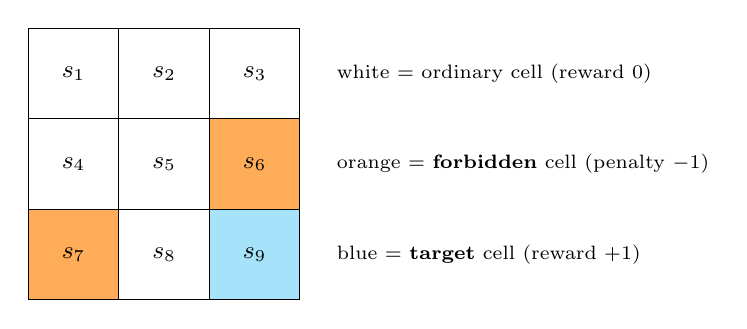
\begin{tikzpicture}[scale=1.15, every node/.style={font=\small}]
  \fill[orange!65] (2,1) rectangle (3,2);
  \fill[orange!65] (0,0) rectangle (1,1);
  \fill[cyan!35]   (2,0) rectangle (3,1);
  \draw[step=1cm, black, thin] (0,0) grid (3,3);
  \node at (0.5,2.5) {$s_1$}; \node at (1.5,2.5) {$s_2$}; \node at (2.5,2.5) {$s_3$};
  \node at (0.5,1.5) {$s_4$}; \node at (1.5,1.5) {$s_5$}; \node at (2.5,1.5) {$s_6$};
  \node at (0.5,0.5) {$s_7$}; \node at (1.5,0.5) {$s_8$}; \node at (2.5,0.5) {$s_9$};
  \node[anchor=west, font=\scriptsize] at (3.3,2.5) {white $=$ ordinary cell (reward $0$)};
  \node[anchor=west, font=\scriptsize] at (3.3,1.5) {orange $=$ \textbf{forbidden} cell (penalty $-1$)};
  \node[anchor=west, font=\scriptsize] at (3.3,0.5) {blue $=$ \textbf{target} cell (reward $+1$)};
\end{tikzpicture}
\end{center}

\begin{remark}[What makes something a state?]
A state must contain \emph{everything relevant about the present}. Here the cell
index is enough: knowing you are at $s_5$ tells you all you need in order to decide
what to do next --- the route you took to arrive there is irrelevant. That property
has a name, the \textbf{Markov property} \bkin{\S1.7, p.~11}, and without it none of
the mathematics in this book would work.

A counterexample makes it concrete. If the grid had a door that opens only once you
have picked up a key, then ``which cell I am in'' would \emph{not} be a valid state
--- two agents in the same cell would face different futures depending on whether
they hold the key. The fix is to enlarge the state to (cell, key held or not).
\end{remark}

% ------------------------------------------------------------
\subsection*{2. The action $a$}
% ------------------------------------------------------------

\bk{\S1.2, p.~2}

\begin{definition}
An \textbf{action} $a$ is a choice available to the agent. The set of actions
available at state $s$ is the \textbf{action space} $\Aspace(s)$.
\end{definition}

In the grid world there are five actions at every state:

\begin{center}
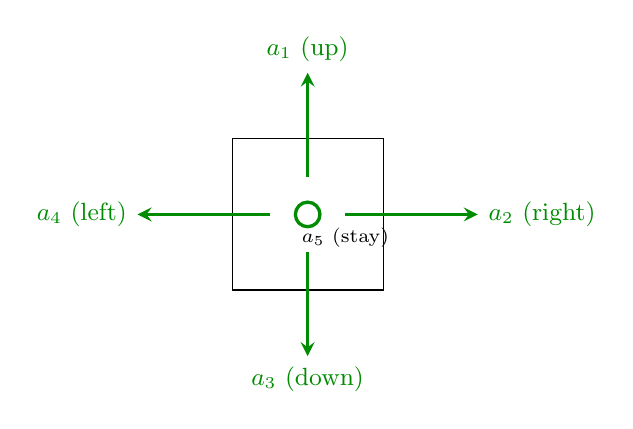
\begin{tikzpicture}[scale=1.2, >=stealth, every node/.style={font=\small}]
  \draw (0,0) rectangle (1.6,1.6);
  \draw[->, very thick, green!55!black] (0.8,1.2) -- (0.8,2.3) node[above] {$a_1$ (up)};
  \draw[->, very thick, green!55!black] (1.2,0.8) -- (2.6,0.8) node[right] {$a_2$ (right)};
  \draw[->, very thick, green!55!black] (0.8,0.4) -- (0.8,-0.7) node[below] {$a_3$ (down)};
  \draw[->, very thick, green!55!black] (0.4,0.8) -- (-1.0,0.8) node[left] {$a_4$ (left)};
  \draw[very thick, green!55!black] (0.8,0.8) circle (0.13);
  \node[font=\scriptsize] at (1.2,0.55) {$a_5$ (stay)};
\end{tikzpicture}
\end{center}

\begin{warning}[Three things that trip people up]
\textbf{(i) Actions are attempts, not outcomes.} Taking $a_1$ at $s_1$ (the top-left
corner) does not move you out of the grid --- you are bounced back to $s_1$ and
collect a reward of $-1$ \bkin{\S1.3, p.~3}. The action is what you \emph{try}; the
environment decides what happens.

\textbf{(ii) Every action is available at every state.} You might think ``left''
should be removed at $s_1$ since it hits a wall. The book deliberately keeps
$\Aspace(s)=\{a_1,\dots,a_5\}$ everywhere and punishes wall-bumping with a negative
reward instead \bkin{\S1.2, p.~2}. This keeps all the tables rectangular.

\textbf{(iii) Actions can be taken into forbidden cells.} Orange cells are enterable,
just unpleasant \bkin{\S1.3, p.~3}. Whether entering one is worth it is exactly the
kind of question values are designed to answer.
\end{warning}

% ------------------------------------------------------------
\subsection*{3. The policy $\pi$}
% ------------------------------------------------------------

\bk{\S1.4, p.~4}

\begin{definition}
A \textbf{policy} $\pi$ tells the agent which action to take at every state.
Formally, $\pi(a\mid s)$ is the probability of taking action $a$ when in state $s$,
and it must satisfy
\[
  \pi(a\mid s)\ \ge\ 0 \quad\text{for all } a,
  \qquad\qquad
  \sum_{a\in\Aspace(s)}\pi(a\mid s)\ =\ 1
  \quad\text{for every } s .
\]
\end{definition}

\begin{intuition}
A policy is a \emph{complete contingency plan}: it specifies what to do at
\emph{every} state, not just the one you happen to occupy. Think of it as a strategy
handed to you before the game starts, covering every situation you might find
yourself in. It is not a route of the form ``go right, then down, then right''; it is
a lookup rule, ``if at $s_5$, go down''.
\end{intuition}

\paragraph{A deterministic policy.} Every state has exactly one arrow, so
$\pi(a\mid s)=1$ for that action and $0$ for the other four:

\begin{center}
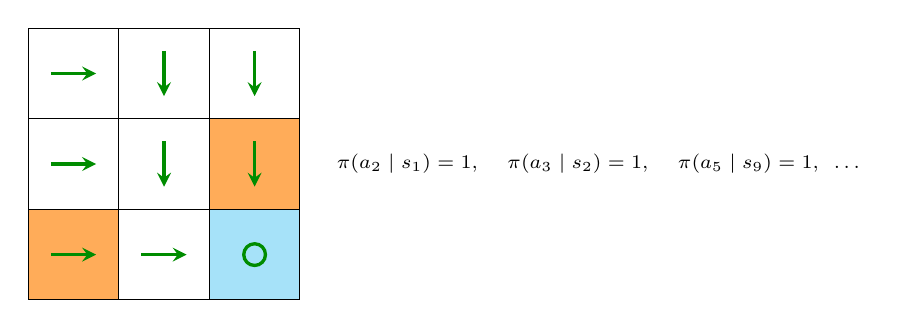
\begin{tikzpicture}[scale=1.15, >=stealth, every node/.style={font=\small}]
  \fill[orange!65] (2,1) rectangle (3,2);
  \fill[orange!65] (0,0) rectangle (1,1);
  \fill[cyan!35]   (2,0) rectangle (3,1);
  \draw[step=1cm, black, thin] (0,0) grid (3,3);
  \draw[->, very thick, green!55!black] (0.25,2.5) -- (0.75,2.5);
  \draw[->, very thick, green!55!black] (1.5,2.75) -- (1.5,2.25);
  \draw[->, very thick, green!55!black] (2.5,2.75) -- (2.5,2.25);
  \draw[->, very thick, green!55!black] (0.25,1.5) -- (0.75,1.5);
  \draw[->, very thick, green!55!black] (1.5,1.75) -- (1.5,1.25);
  \draw[->, very thick, green!55!black] (2.5,1.75) -- (2.5,1.25);
  \draw[->, very thick, green!55!black] (0.25,0.5) -- (0.75,0.5);
  \draw[->, very thick, green!55!black] (1.25,0.5) -- (1.75,0.5);
  \draw[very thick, green!55!black] (2.5,0.5) circle (0.12);
  \node[anchor=west, font=\scriptsize] at (3.3,1.5)
    {$\pi(a_2\mid s_1)=1$, \quad $\pi(a_3\mid s_2)=1$, \quad $\pi(a_5\mid s_9)=1$, \ \dots};
\end{tikzpicture}
\end{center}

\paragraph{A stochastic policy.} At $s_1$ the agent now tosses a fair coin between
going right and going down; everywhere else it is unchanged:

\begin{center}
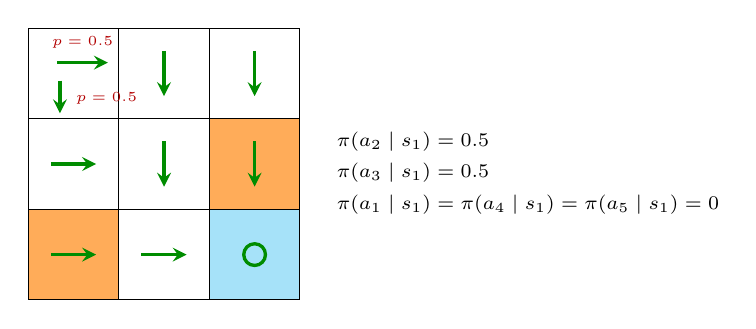
\begin{tikzpicture}[scale=1.15, >=stealth, every node/.style={font=\small}]
  \fill[orange!65] (2,1) rectangle (3,2);
  \fill[orange!65] (0,0) rectangle (1,1);
  \fill[cyan!35]   (2,0) rectangle (3,1);
  \draw[step=1cm, black, thin] (0,0) grid (3,3);
  \draw[->, very thick, green!55!black] (0.32,2.62) -- (0.88,2.62);
  \node[font=\tiny, red!70!black] at (0.6,2.84) {$p=0.5$};
  \draw[->, very thick, green!55!black] (0.35,2.42) -- (0.35,2.06);
  \node[font=\tiny, red!70!black, anchor=west] at (0.42,2.22) {$p=0.5$};
  \draw[->, very thick, green!55!black] (1.5,2.75) -- (1.5,2.25);
  \draw[->, very thick, green!55!black] (2.5,2.75) -- (2.5,2.25);
  \draw[->, very thick, green!55!black] (0.25,1.5) -- (0.75,1.5);
  \draw[->, very thick, green!55!black] (1.5,1.75) -- (1.5,1.25);
  \draw[->, very thick, green!55!black] (2.5,1.75) -- (2.5,1.25);
  \draw[->, very thick, green!55!black] (0.25,0.5) -- (0.75,0.5);
  \draw[->, very thick, green!55!black] (1.25,0.5) -- (1.75,0.5);
  \draw[very thick, green!55!black] (2.5,0.5) circle (0.12);
  \node[anchor=west, font=\scriptsize] at (3.3,1.75) {$\pi(a_2\mid s_1)=0.5$};
  \node[anchor=west, font=\scriptsize] at (3.3,1.40) {$\pi(a_3\mid s_1)=0.5$};
  \node[anchor=west, font=\scriptsize] at (3.3,1.05) {$\pi(a_1\mid s_1)=\pi(a_4\mid s_1)=\pi(a_5\mid s_1)=0$};
\end{tikzpicture}
\end{center}

\begin{remark}[Policy versus trajectory]
Running a policy produces a \textbf{trajectory} --- an actual sequence of states,
actions and rewards, such as
$s_1\xrightarrow{a_2}s_2\xrightarrow{a_3}s_5\xrightarrow{a_3}s_8\xrightarrow{a_2}s_9$.
The policy is the \emph{rule}; the trajectory is one \emph{realisation} of it. A
deterministic policy in a deterministic environment always produces the same
trajectory from a given start; a stochastic policy produces a different one each time
\bkin{\S1.6, p.~8}.
\end{remark}

% ------------------------------------------------------------
\subsection*{4. The state value $v_\pi(s)$}
% ------------------------------------------------------------

\bk{\S2.3, p.~19}

This is the one that needs the most care, so we build it in three steps.

\paragraph{Step 1: reward $r$ --- what you get right now.} After taking an action you
receive a number. In the grid world: $-1$ for hitting the boundary, $-1$ for entering
a forbidden cell, $+1$ for reaching the target, $0$ otherwise \bkin{\S1.5, p.~7}.

\paragraph{Step 2: return $G_t$ --- what you get in total.} A single reward is
myopic; what matters is the whole future stream, with later rewards discounted
\bkin{\S1.6, p.~9}:
\[
  G_t \;=\; R_{t+1} + \gamma R_{t+2} + \gamma^2 R_{t+3} + \cdots,
  \qquad \gamma\in(0,1).
\]
The discount rate $\gamma$ plays exactly the role an economist expects: it is a
one-period discount factor, and $1/(1-\gamma)$ is the present value of a perpetuity
paying $1$ per period.

\paragraph{Step 3: state value $v_\pi(s)$ --- what you get on average.} The return is
a random variable, because the policy and the environment may both be stochastic.
Average it:

\begin{definition}[State value]
\[
  \boxed{\;v_\pi(s)\;=\;\E\bigl[G_t \,\big|\, S_t=s\bigr]\;}
\]
the expected discounted return obtained by \emph{starting at $s$ and following $\pi$
forever afterwards}.
\end{definition}

\begin{warning}[Read the subscript]
$v_\pi$ carries a $\pi$ for a reason. \textbf{A state has no value on its own} ---
only a value \emph{under a given policy}. The same cell $s_1$ is worth a lot under a
good policy and very little under a bad one. Asking ``what is the value of $s_1$?''
is like asking ``what is this chess position worth?'' without saying who is playing.
\end{warning}

\subsubsection*{A fully worked value computation}

Take the smallest example that shows everything \bkin{\S2.5, pp.~22--25}. A
$2\times2$ grid: $s_2$ is forbidden, $s_4$ is the target, $\gamma=0.9$. Consider the
policy drawn below --- at $s_1$ go down, at $s_2$ go down, at $s_3$ go right, at $s_4$
stay put.

\begin{center}
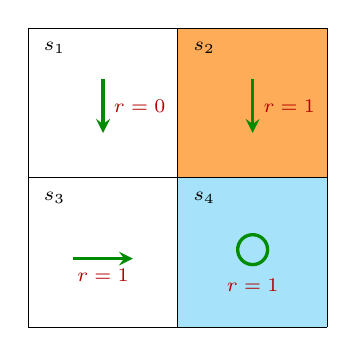
\begin{tikzpicture}[scale=1.9, >=stealth, every node/.style={font=\small},
                    rw/.style={font=\scriptsize, red!70!black}]
  \fill[orange!65] (1,1) rectangle (2,2);
  \fill[cyan!35]   (1,0) rectangle (2,1);
  \draw[step=1cm, black, thin] (0,0) grid (2,2);
  \node[font=\scriptsize, anchor=north west] at (0.04,1.97) {$s_1$};
  \node[font=\scriptsize, anchor=north west] at (1.04,1.97) {$s_2$};
  \node[font=\scriptsize, anchor=north west] at (0.04,0.97) {$s_3$};
  \node[font=\scriptsize, anchor=north west] at (1.04,0.97) {$s_4$};
  \draw[->, very thick, green!55!black] (0.5,1.66) -- (0.5,1.30)
        node[midway, right, rw] {$r=0$};
  \draw[->, very thick, green!55!black] (1.5,1.66) -- (1.5,1.30)
        node[midway, right, rw] {$r=1$};
  \draw[->, very thick, green!55!black] (0.30,0.46) -- (0.70,0.46)
        node[midway, below, rw] {$r=1$};
  \draw[very thick, green!55!black] (1.5,0.52) circle (0.10);
  \node[rw] at (1.5,0.28) {$r=1$};
\end{tikzpicture}
\end{center}

\textbf{Write down one equation per state.} Each says: value $=$ immediate reward
$+\ \gamma\times$ value of wherever you land.
\[
  v_\pi(s_1)=0+\gamma v_\pi(s_3),\qquad
  v_\pi(s_2)=1+\gamma v_\pi(s_4),
\]
\[
  v_\pi(s_3)=1+\gamma v_\pi(s_4),\qquad
  v_\pi(s_4)=1+\gamma v_\pi(s_4).
\]

\textbf{Solve.} The last equation involves only $v_\pi(s_4)$:
\[
  v_\pi(s_4)=1+\gamma v_\pi(s_4)
  \ \Longrightarrow\ v_\pi(s_4)(1-\gamma)=1
  \ \Longrightarrow\ v_\pi(s_4)=\frac{1}{1-\gamma}=\frac{1}{0.1}=10 .
\]
Then back-substitute:
\[
  v_\pi(s_3)=1+0.9(10)=10,\qquad
  v_\pi(s_2)=1+0.9(10)=10,\qquad
  v_\pi(s_1)=0+0.9(10)=9 .
\]

\begin{center}
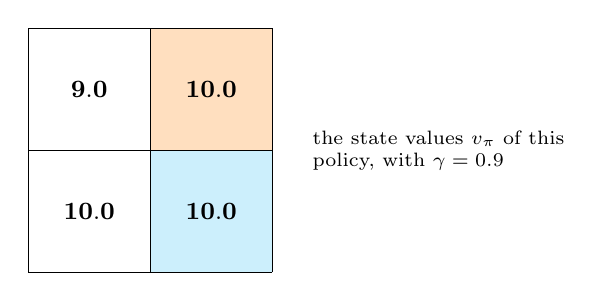
\begin{tikzpicture}[scale=1.55, every node/.style={font=\small}]
  \fill[orange!25] (1,1) rectangle (2,2);
  \fill[cyan!20]   (1,0) rectangle (2,1);
  \draw[step=1cm, black, thin] (0,0) grid (2,2);
  \node at (0.5,1.5) {$\mathbf{9.0}$};  \node at (1.5,1.5) {$\mathbf{10.0}$};
  \node at (0.5,0.5) {$\mathbf{10.0}$}; \node at (1.5,0.5) {$\mathbf{10.0}$};
  \node[anchor=west, font=\scriptsize, align=left] at (2.25,1.0)
    {the state values $v_\pi$ of this\\ policy, with $\gamma=0.9$};
\end{tikzpicture}
\end{center}

\begin{intuition}[Why $s_1$ is worth less]
$s_1$ scores $9$ rather than $10$ purely because it sits one step further from the
reward: the $+1$ stream starts one period later and is therefore discounted once
more. Nothing bad happens at $s_1$ --- it is simply further away. This is the ordinary
logic of a present-value calculation.
\end{intuition}

\subsubsection*{Values rank policies --- which is the whole point}

Now change one thing: at $s_1$, send the agent \emph{right} into the forbidden cell
($r=-1$) instead of down. Redoing the arithmetic \bkin{\S3.1, p.~36}:
\[
  v_\pi(s_1)=-1+\gamma v_\pi(s_2)=-1+0.9(10)=8 .
\]

\begin{center}
\small
\begin{tabular}{@{}lcccc@{}}
\toprule
& $v_\pi(s_1)$ & $v_\pi(s_2)$ & $v_\pi(s_3)$ & $v_\pi(s_4)$\\
\midrule
Policy A (at $s_1$ go down)  & $\mathbf{9}$ & 10 & 10 & 10\\
Policy B (at $s_1$ go right) & $8$          & 10 & 10 & 10\\
\bottomrule
\end{tabular}
\end{center}

Policy A is at least as good at every state and strictly better at $s_1$, so
\textbf{A is the better policy} --- and we reached that verdict by arithmetic, not by
eyeballing the picture. That is what state values are \emph{for}
\bkin{\S2.5, p.~25}.

% ------------------------------------------------------------
\subsection*{How the four objects chain together}
% ------------------------------------------------------------

\begin{center}
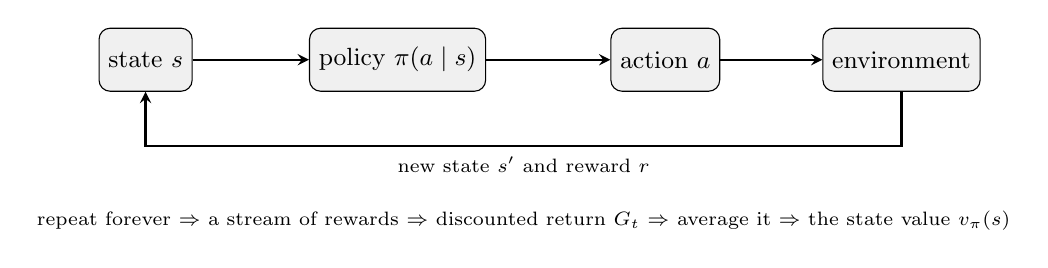
\begin{tikzpicture}[>=stealth, every node/.style={font=\small}]
  \node[draw, rounded corners, fill=gray!12, minimum height=8mm] (s) at (0,0) {state $s$};
  \node[draw, rounded corners, fill=gray!12, minimum height=8mm] (p) at (3.2,0) {policy $\pi(a\mid s)$};
  \node[draw, rounded corners, fill=gray!12, minimum height=8mm] (a) at (6.6,0) {action $a$};
  \node[draw, rounded corners, fill=gray!12, minimum height=8mm] (e) at (9.6,0) {environment};
  \draw[->, thick] (s) -- (p);
  \draw[->, thick] (p) -- (a);
  \draw[->, thick] (a) -- (e);
  \draw[->, thick] (e.south) -- (9.6,-1.1) -- node[below, font=\scriptsize]
        {new state $s'$ and reward $r$} (0,-1.1) -- (s.south);
  \node[font=\scriptsize, align=center] at (4.8,-2.05)
        {repeat forever $\Rightarrow$ a stream of rewards $\Rightarrow$ discounted return $G_t$
         $\Rightarrow$ average it $\Rightarrow$ the state value $v_\pi(s)$};
\end{tikzpicture}
\end{center}

Formally the chain is \bkin{\S2.4, p.~21}
\[
  v_\pi(s)=\underbrace{\sum_{a}\pi(a\mid s)}_{\text{which action --- from the \emph{policy}}}
  \Bigl[\underbrace{\sum_r p(r\mid s,a)\,r}_{\text{reward now}}
  +\ \gamma\underbrace{\sum_{s'}p(s'\mid s,a)\,v_\pi(s')}_{\text{value of the next \emph{state}}}\Bigr],
\]
which is the Bellman equation --- and you can now read every symbol in it.

% ------------------------------------------------------------
\subsection*{Six confusions worth heading off}
% ------------------------------------------------------------

\begin{enumerate}
  \item \textbf{Reward vs.\ return vs.\ value.} \emph{Reward} is one number received
        once. \emph{Return} is the discounted sum of all future rewards along one
        trajectory --- still random. \emph{Value} is the expectation of the return ---
        a fixed number. Reward is myopic and cannot rank policies; value can
        \bkin{\S1.5, p.~7}.

  \item \textbf{A policy is not a path.} It is a rule defined at every state, so the
        agent still knows what to do if it is blown off course.

  \item \textbf{Value depends on the policy.} Always $v_\pi$, never $v$ alone ---
        except for $v^*$, the value of an \emph{optimal} policy \bkin{\S3.2, p.~38}.

  \item \textbf{State value vs.\ action value.} $v_\pi(s)$ answers ``how good is it to
        be here, behaving as usual?'' The \textbf{action value}
        $q_\pi(s,a)=\E[G_t\mid S_t=s,A_t=a]$ answers ``how good is it to be here and
        do $a$ \emph{once}, then behave as usual?'' They are linked by
        $v_\pi(s)=\sum_a\pi(a\mid s)q_\pi(s,a)$ \bkin{\S2.8, p.~30}. Improving a policy
        means comparing $q$ values, which is why $q$ takes over from $v$ later in the
        book.

  \item \textbf{$\pi(a\mid s)$ and $p(s'\mid s,a)$ are different objects.} The policy
        belongs to the \emph{agent} and is what we optimise. The transition
        probability belongs to the \emph{environment} and is not ours to choose ---
        indeed from Chapter 5 onward we do not even know it.

  \item \textbf{Action values exist for actions your policy never takes.} If $\pi$
        never picks $a$ at $s$, $q_\pi(s,a)$ is still perfectly well defined, and it
        may well be the largest of them all --- which is precisely how a policy gets
        improved \bkin{\S2.8.1, p.~32}.
\end{enumerate}

\begin{center}
\small
\begin{tabular}{@{}lll@{}}
\toprule
Object & Type & Grid-world instance \\
\midrule
$s$ & element of $\Sspace$ & $s_5$, the middle cell \\
$a$ & element of $\Aspace(s)$ & $a_3$, ``move down'' \\
$\pi(a\mid s)$ & a probability distribution over $a$, for each $s$ & $\pi(a_3\mid s_5)=1$ \\
$r$ & a real number & $-1$ for entering a forbidden cell \\
$G_t$ & a random variable & $0+\gamma 0+\gamma^2 1+\cdots$ \\
$v_\pi(s)$ & a real number, one per state & $v_\pi(s_1)=9$ when $\gamma=0.9$ \\
$q_\pi(s,a)$ & a real number, one per state--action pair & $q_\pi(s_1,a_3)=9$ \\
\bottomrule
\end{tabular}
\end{center}

\newpage

% ============================================================
\section{Basic Concepts}
% ============================================================

\begin{roadmap}{Chapter 1 of the textbook}
\textbf{Textbook:} Chapter 1, ``Basic Concepts'', pp.~1--13.
Sections: \S1.1 grid world (p.~1), \S1.2 state and action (p.~2), \S1.3 state
transition (p.~3), \S1.4 policy (p.~4), \S1.5 reward (p.~6), \S1.6 trajectories,
returns, episodes (p.~8), \S1.7 Markov decision processes (p.~11),
\S1.8 summary (p.~12), \S1.9 Q\&A (p.~12).\\[0.3em]
\textbf{Videos:}
\vid{Overview of RL in 30 minutes}{https://www.youtube.com/watch?v=ZHMWHr9811U};
\vid{L1 P1 --- State, action, policy}{https://www.youtube.com/watch?v=zJHtM5dN69g};
\vid{L1 P2 --- Reward, return, MDP}{https://www.youtube.com/watch?v=repVl3_GYCI}.\\[0.3em]
\textbf{What to take away:} the seven primitives (state, action, state transition,
policy, reward, return, episode) and how they assemble into a Markov decision
process.
\end{roadmap}

\begin{figure}[htbp]
  \centering
  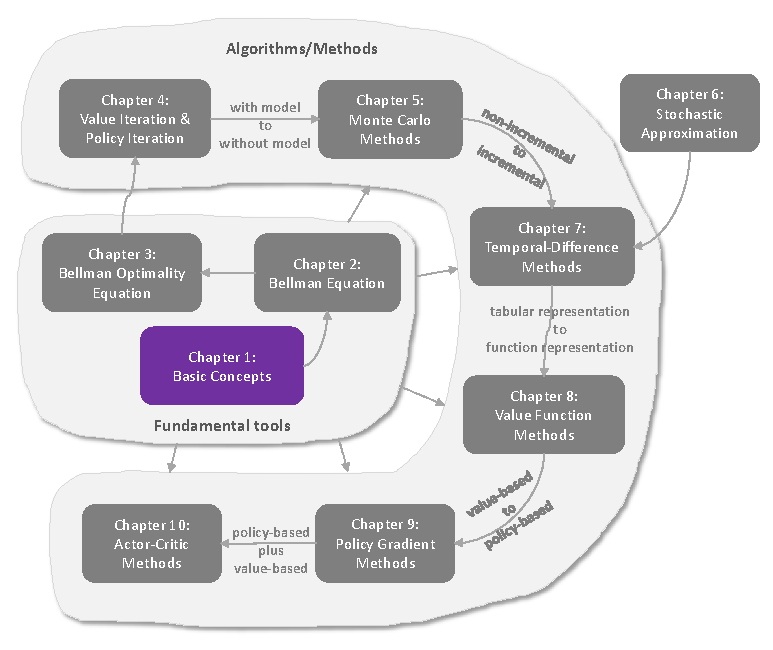
\includegraphics[width=371.3pt]{fig1_1}\par\smallskip
  \begin{minipage}{0.94\textwidth}\footnotesize
  \textbf{Figure 1.1.} Where we are in this book.\par\smallskip
  \textcolor{rulegray}{\scriptsize Reproduced from S.~Zhao, \emph{Mathematical Foundations of Reinforcement Learning} (Springer, 2025).}
  \end{minipage}
\end{figure}


\subsection{The grid world, once and for all}

\bk{\S1.1, p.~1; Figure 1.2, p.~2}

Almost every example in the textbook is a \emph{grid world}. A robot (the
\textbf{agent}) sits in one cell of a rectangular grid. White cells are ordinary,
orange cells are \textbf{forbidden}, and one blue cell is the \textbf{target}. At
each time step the agent occupies exactly one cell and chooses a move. The goal is
to find a rule for choosing moves that gets the agent to the target from any
starting cell, without entering forbidden cells, without pointless detours, and
without banging into the outer wall.

The reason the book uses one running example for ten chapters is worth stating
plainly: it means that when an algorithm changes, you can see exactly what changed,
because the problem did not. Get comfortable with this grid; you will see it a
hundred times.

\begin{intuition}
If the agent had a map, this would be a shortest-path problem and you would solve
it with Dijkstra's algorithm in an afternoon. RL is what you do when the agent has
\emph{no map}: it must discover the layout by trying things and observing what
happens. Everything hard about RL follows from that one missing ingredient
\bkin{\S1.1, p.~1}.
\end{intuition}

\begin{figure}[htbp]
  \centering
  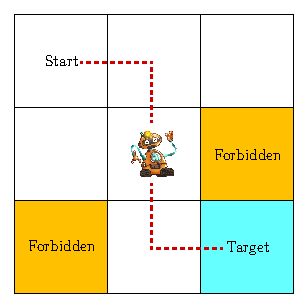
\includegraphics[width=147.7pt]{fig1_2}\par\smallskip
  \begin{minipage}{0.94\textwidth}\footnotesize
  \textbf{Figure 1.2.} The grid world example is used throughout the book.\par\smallskip
  \textcolor{rulegray}{\scriptsize Reproduced from S.~Zhao, \emph{Mathematical Foundations of Reinforcement Learning} (Springer, 2025).}
  \end{minipage}
\end{figure}


\subsection{State and action}

\bk{\S1.2, p.~2; Figure 1.3, p.~3}

\begin{definition}
A \textbf{state} $s$ describes the agent's status with respect to the environment.
The set of all states is the \textbf{state space} $\Sspace$.
\end{definition}

In the $3\times3$ grid there are nine cells and therefore nine states,
$\Sspace=\{s_1,\dots,s_9\}$, indexed left to right, top to bottom.

\begin{definition}
An \textbf{action} $a$ is a choice available to the agent. The set of actions at
state $s$ is the \textbf{action space} $\Aspace(s)$.
\end{definition}

The grid world has five actions:
$a_1$ = up, $a_2$ = right, $a_3$ = down, $a_4$ = left, $a_5$ = stay still.

\begin{remark}
In principle the action space can differ across states. For example, at the
top-left corner $s_1$ both ``up'' and ``left'' would run into the wall, so you
could declare $\Aspace(s_1)=\{a_2,a_3,a_5\}$. The textbook deliberately does
\emph{not} do this: it keeps $\Aspace(s_i)=\Aspace=\{a_1,\dots,a_5\}$ for every
state, and instead punishes wall-bumping with a negative reward
\bkin{\S1.2, p.~2}. This is the more general setup and it keeps all the tables
rectangular.
\end{remark}

\begin{figure}[htbp]
  \centering
  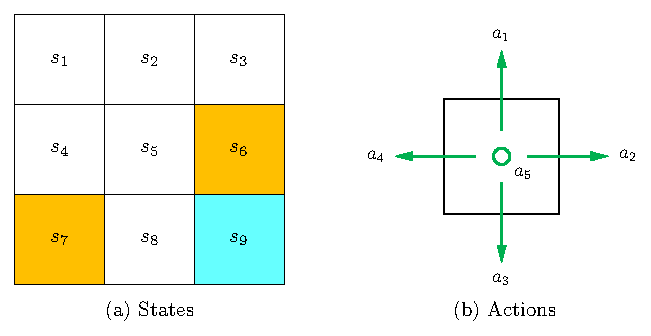
\includegraphics[width=312.5pt]{fig1_3}\par\smallskip
  \begin{minipage}{0.94\textwidth}\footnotesize
  \textbf{Figure 1.3.} Illustrations of the state and action concepts. (a) There are nine states \{s1, . . . , s9\}. (b) Each state has five possible actions \{a1, a2, a3, a4, a5\}.\par\smallskip
  \textcolor{rulegray}{\scriptsize Reproduced from S.~Zhao, \emph{Mathematical Foundations of Reinforcement Learning} (Springer, 2025).}
  \end{minipage}
\end{figure}


\subsection{State transition}

\bk{\S1.3, p.~3; Table 1.1, p.~4}

Taking an action moves the agent from one state to another. Write
$s_1 \xrightarrow{a_2} s_2$ for ``taking $a_2$ at $s_1$ leads to $s_2$''.

Two edge cases are settled once and for all in the textbook:

\begin{itemize}
  \item \textbf{Walking into the outer boundary.} The agent is bounced back:
        $s_1 \xrightarrow{a_1} s_1$. It cannot leave the state space.
  \item \textbf{Walking into a forbidden cell.} Two modelling choices exist: the
        forbidden cell is a wall (agent bounces back) or the forbidden cell is
        enterable but unpleasant. \emph{The book chooses the second}: forbidden
        cells are accessible, entering them earns a penalty
        \bkin{\S1.3, p.~3}.
\end{itemize}

\begin{definition}
The \textbf{state transition probability} is
\[
  p(s'\mid s,a) = \Prob(S_{t+1}=s' \mid S_t=s,\ A_t=a),
  \qquad \sum_{s'\in\Sspace} p(s'\mid s,a)=1 \ \ \forall (s,a).
\]
\end{definition}

For the deterministic grid, $p(s_2\mid s_1,a_2)=1$ and $p(s'\mid s_1,a_2)=0$ for
every other $s'$. A tabular listing (the book's Table 1.1) captures this perfectly.
But a table can only express \emph{deterministic} transitions. The conditional
probability notation is strictly more general: with random wind gusts, taking $a_2$
at $s_1$ might blow the agent to $s_5$, i.e.\ $p(s_5\mid s_1,a_2)>0$
\bkin{\S1.3, p.~4}.

\begin{worked}{reading the transition table}
From the book's Table 1.1 (p.~4), row $s_5$ reads: $a_1\to s_2$, $a_2\to s_6$,
$a_3\to s_8$, $a_4\to s_4$, $a_5\to s_5$. Note $a_2\to s_6$ even though $s_6$ is a
forbidden cell --- consistent with the ``forbidden cells are accessible'' choice
above. Row $s_9$ reads $a_1\to s_6$, $a_2\to s_9$, $a_3\to s_9$, $a_4\to s_8$,
$a_5\to s_9$: three of the five actions leave the agent where it is, because $s_9$
is the bottom-right corner.
\end{worked}

\begin{table}[htbp]\centering\footnotesize
\begin{tabular}{@{}l|ccccc@{}}
\toprule
 & $a_1$ (up) & $a_2$ (right) & $a_3$ (down) & $a_4$ (left) & $a_5$ (stay)\\
\midrule
$s_1$ & $s_1$ & $s_2$ & $s_4$ & $s_1$ & $s_1$\\
$s_2$ & $s_2$ & $s_3$ & $s_5$ & $s_1$ & $s_2$\\
$s_3$ & $s_3$ & $s_3$ & $s_6$ & $s_2$ & $s_3$\\
$s_4$ & $s_1$ & $s_5$ & $s_7$ & $s_4$ & $s_4$\\
$s_5$ & $s_2$ & $s_6$ & $s_8$ & $s_4$ & $s_5$\\
$s_6$ & $s_3$ & $s_6$ & $s_9$ & $s_5$ & $s_6$\\
$s_7$ & $s_4$ & $s_8$ & $s_7$ & $s_7$ & $s_7$\\
$s_8$ & $s_5$ & $s_9$ & $s_8$ & $s_7$ & $s_8$\\
$s_9$ & $s_6$ & $s_9$ & $s_9$ & $s_8$ & $s_9$\\
\bottomrule
\end{tabular}\par\smallskip
{\footnotesize\textbf{Table 1.1.} Tabular representation of the state transition process: each cell gives
the next state reached by taking that action at that state \bkin{\S1.3, p.~4}.}
\end{table}


\subsection{Policy}

\bk{\S1.4, p.~4; Figures 1.4--1.5, pp.~5--6; Table 1.2, p.~6}

\begin{definition}
A \textbf{policy} $\pi$ tells the agent which action to take at every state.
Formally $\pi(a\mid s)$ is the probability of taking $a$ at $s$, with
$\sum_{a\in\Aspace(s)}\pi(a\mid s)=1$ for every $s$.
\end{definition}

A policy is drawn as a field of arrows, one arrow per cell. Two kinds:

\begin{itemize}
  \item \textbf{Deterministic}: $\pi(a^*\mid s)=1$ for one action $a^*$. Example
        from the book: $\pi(a_2\mid s_1)=1$ and $\pi(a\mid s_1)=0$ for $a\neq a_2$
        \bkin{\S1.4, p.~5}.
  \item \textbf{Stochastic}: several actions get positive probability. The book's
        Figure 1.5 (p.~6) has $\pi(a_2\mid s_1)=\pi(a_3\mid s_1)=0.5$, drawn as two
        arrows each labelled $p=0.5$.
\end{itemize}

A policy stored as a table with one row per state and one column per action is
called a \textbf{tabular representation} \bkin{\S1.4, p.~6}. Keep this word in mind:
Chapters 1--7 all use tabular representations, and Chapters 8--10 are precisely
about replacing the table with a parameterised function.

\begin{remark}
Note the asymmetry in notation: $p(s'\mid s,a)$ belongs to the \emph{environment}
and is not ours to choose; $\pi(a\mid s)$ belongs to the \emph{agent} and is exactly
the thing we are trying to optimise.
\end{remark}

\begin{figure}[htbp]
  \centering
  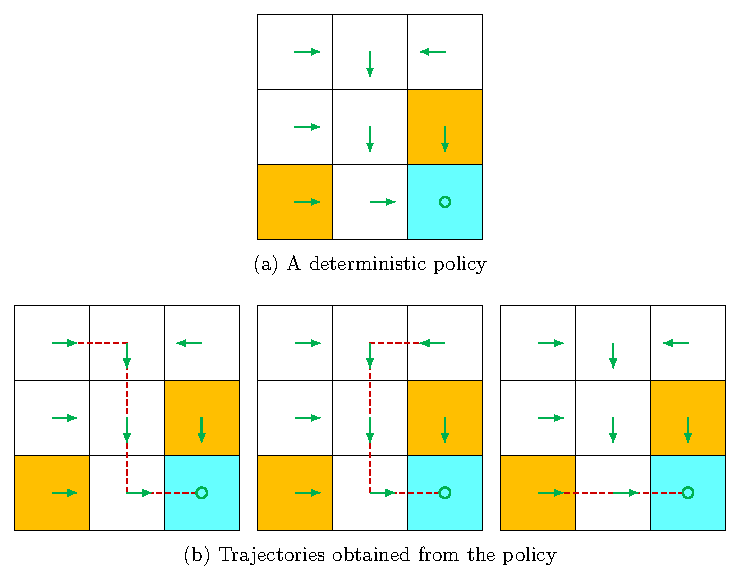
\includegraphics[width=355.2pt]{fig1_4}\par\smallskip
  \begin{minipage}{0.94\textwidth}\footnotesize
  \textbf{Figure 1.4.} A policy represented by arrows and some trajectories obtained by starting from different initial states.\par\smallskip
  \textcolor{rulegray}{\scriptsize Reproduced from S.~Zhao, \emph{Mathematical Foundations of Reinforcement Learning} (Springer, 2025).}
  \end{minipage}
\end{figure}


\begin{figure}[htbp]
  \centering
  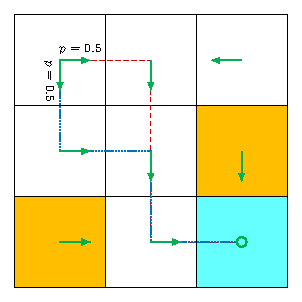
\includegraphics[width=144.8pt]{fig1_5}\par\smallskip
  \begin{minipage}{0.94\textwidth}\footnotesize
  \textbf{Figure 1.5.} A stochastic policy. In state s1, the agent may move rightward or downward with equal probabilities of 0.5.\par\smallskip
  \textcolor{rulegray}{\scriptsize Reproduced from S.~Zhao, \emph{Mathematical Foundations of Reinforcement Learning} (Springer, 2025).}
  \end{minipage}
\end{figure}


\begin{table}[htbp]\centering\footnotesize
\begin{tabular}{@{}l|ccccc@{}}
\toprule
 & $a_1$ (up) & $a_2$ (right) & $a_3$ (down) & $a_4$ (left) & $a_5$ (stay)\\
\midrule
$s_1$ & 0 & 0.5 & 0.5 & 0 & 0\\
$s_2$ & 0 & 0 & 1 & 0 & 0\\
$s_3$ & 0 & 0 & 0 & 1 & 0\\
$s_4$ & 0 & 1 & 0 & 0 & 0\\
$s_5$ & 0 & 0 & 1 & 0 & 0\\
$s_6$ & 0 & 0 & 1 & 0 & 0\\
$s_7$ & 0 & 1 & 0 & 0 & 0\\
$s_8$ & 0 & 1 & 0 & 0 & 0\\
$s_9$ & 0 & 0 & 0 & 0 & 1\\
\bottomrule
\end{tabular}\par\smallskip
{\footnotesize\textbf{Table 1.2.} Tabular representation of the stochastic policy of Figure 1.5: entry
$(i,j)$ is the probability of taking action $a_j$ at state $s_i$ \bkin{\S1.4, p.~6}.}
\end{table}


\subsection{Reward}

\bk{\S1.5, p.~6; Table 1.3, p.~8}

\begin{definition}
After executing action $a$ at state $s$, the agent receives a scalar
\textbf{reward} $r$, a real number that may be positive, negative or zero. In
general it is described by the conditional distribution $p(r\mid s,a)$ with
$\sum_r p(r\mid s,a)=1$.
\end{definition}

The book's standard grid-world reward design \bkin{\S1.5, p.~7}:
\[
  r_{\text{boundary}}=-1,\qquad
  r_{\text{forbidden}}=-1,\qquad
  r_{\text{target}}=+1,\qquad
  r_{\text{other}}=0.
\]

Three points that beginners routinely get wrong.

\begin{warning}
\textbf{(i) Rewards are not the objective.} If you hand a student the reward table
and ask them to build a policy by picking, at each state, the action with the
largest immediate reward, they will build a bad policy. Immediate reward is
myopic; what matters is the \emph{total} reward accumulated in the long run. The
book states this explicitly \bkin{\S1.5, p.~7}. This is the entire reason state
values exist.

\textbf{(ii) The reward at the target does not stop the process.} At $s_9$ the
process continues. Taking $a_5$ (stay) at $s_9$ returns you to $s_9$ with
$r=+1$ again; taking $a_2$ at $s_9$ also returns you to $s_9$ but with
$r=r_{\text{boundary}}=-1$, because you tried to leave the grid
\bkin{\S1.5, p.~7}.

\textbf{(iii) Only relative reward values matter.} Adding the same constant to
every reward leaves the optimal policy unchanged. Setting
$r_{\text{boundary}}=r_{\text{forbidden}}=-3,\ r_{\text{target}}=-1,\
r_{\text{other}}=-2$ --- all negative --- gives exactly the same optimal policy
\bkin{\S1.9 Q\&A, p.~12}. The formal statement is Theorem 3.6 (optimal policy
invariance), \bkin{\S3.5, p.~51}, proved in Chapter 3 of these notes.
\end{warning}

\begin{remark}[Does the reward depend on the next state?]
Intuitively, yes: you get $+1$ \emph{because} you landed on the target. So why does
the book write $p(r\mid s,a)$ rather than $p(r\mid s,a,s')$? Because $s'$ is itself
generated by $(s,a)$, so you can always marginalise it out:
\[
  p(r\mid s,a) = \sum_{s'} p(r\mid s,a,s')\, p(s'\mid s,a).
\]
The two formulations are equivalent, and $p(r\mid s,a)$ makes the Bellman equation
cleaner \bkin{\S1.9 Q\&A, p.~13}.
\end{remark}

\begin{table}[htbp]\centering\footnotesize
\setlength{\tabcolsep}{4pt}
\begin{tabular}{@{}l|ccccc@{}}
\toprule
 & $a_1$ (up) & $a_2$ (right) & $a_3$ (down) & $a_4$ (left) & $a_5$ (stay)\\
\midrule
$s_1$ & $r_{\text{bnd}}$ & 0 & 0 & $r_{\text{bnd}}$ & 0\\
$s_2$ & $r_{\text{bnd}}$ & 0 & 0 & 0 & 0\\
$s_3$ & $r_{\text{bnd}}$ & $r_{\text{bnd}}$ & $r_{\text{fbd}}$ & 0 & 0\\
$s_4$ & 0 & 0 & $r_{\text{fbd}}$ & $r_{\text{bnd}}$ & 0\\
$s_5$ & 0 & $r_{\text{fbd}}$ & 0 & 0 & 0\\
$s_6$ & 0 & $r_{\text{bnd}}$ & $r_{\text{tgt}}$ & 0 & $r_{\text{fbd}}$\\
$s_7$ & 0 & 0 & $r_{\text{bnd}}$ & $r_{\text{bnd}}$ & $r_{\text{fbd}}$\\
$s_8$ & 0 & $r_{\text{tgt}}$ & $r_{\text{bnd}}$ & $r_{\text{fbd}}$ & 0\\
$s_9$ & $r_{\text{fbd}}$ & $r_{\text{bnd}}$ & $r_{\text{bnd}}$ & 0 & $r_{\text{tgt}}$\\
\bottomrule
\end{tabular}\par\smallskip
{\footnotesize\textbf{Table 1.3.} Tabular representation of the reward process \bkin{\S1.5, p.~8}. Here
$r_{\text{bnd}}=r_{\text{boundary}}$, $r_{\text{fbd}}=r_{\text{forbidden}}$,
$r_{\text{tgt}}=r_{\text{target}}$.}
\end{table}


\subsection{Trajectories, returns and episodes}

\bk{\S1.6, p.~8; Figure 1.6, p.~8}

A \textbf{trajectory} is a state--action--reward chain. Following the book's
Figure 1.6(a) (p.~8):
\[
  s_1 \xrightarrow[r=0]{a_2} s_2 \xrightarrow[r=0]{a_3} s_5
      \xrightarrow[r=0]{a_3} s_8 \xrightarrow[r=1]{a_2} s_9 .
\]

\begin{definition}
The (undiscounted) \textbf{return} of a trajectory is the sum of rewards collected
along it.
\end{definition}

For the trajectory above, $\text{return}=0+0+0+1=1$ (the book's equation (1.1),
p.~8). Compare with the alternative policy of Figure 1.6(b):
\[
  s_1 \xrightarrow[r=0]{a_3} s_4 \xrightarrow[r=-1]{a_3} s_7
      \xrightarrow[r=0]{a_2} s_8 \xrightarrow[r=+1]{a_2} s_9,
  \qquad \text{return}=0-1+0+1=0,
\]
the book's equation (1.2), p.~9. So $1>0$: the first policy is better. The
mathematics agrees with the intuition that the second policy is worse because it
cuts through a forbidden cell. \emph{This tiny calculation is the seed of the
entire subject}: returns turn ``that policy looks better'' into a number.

\begin{figure}[htbp]
  \centering
  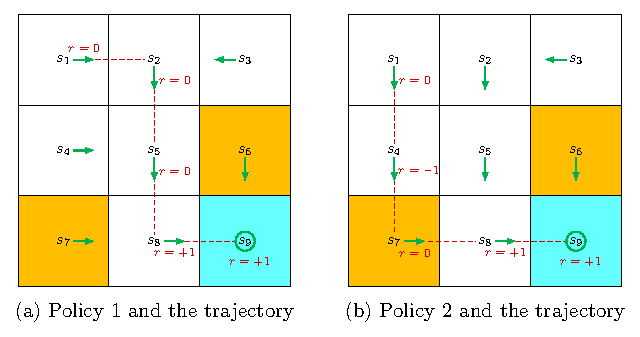
\includegraphics[width=307.2pt]{fig1_6}\par\smallskip
  \begin{minipage}{0.94\textwidth}\footnotesize
  \textbf{Figure 1.6.} Trajectories obtained by following two policies. The trajectories are indicated by red dashed lines.\par\smallskip
  \textcolor{rulegray}{\scriptsize Reproduced from S.~Zhao, \emph{Mathematical Foundations of Reinforcement Learning} (Springer, 2025).}
  \end{minipage}
\end{figure}


\subsubsection*{Why we must discount}

\bk{\S1.6, pp.~9--10, equation (1.3)}

If the agent stays at $s_9$ forever it keeps collecting $+1$:
\[
  \text{return} = 0+0+0+1+1+1+\cdots = \infty,
\]
which diverges and so cannot rank policies. Fix: discount.

\begin{definition}
The \textbf{discounted return} starting at time $t$ is
\[
  G_t \;=\; R_{t+1} + \gamma R_{t+2} + \gamma^2 R_{t+3} + \cdots
      \;=\; \sum_{k=0}^{\infty}\gamma^{k}R_{t+k+1},
  \qquad \gamma\in(0,1),
\]
where $\gamma$ is the \textbf{discount rate}.
\end{definition}

For the trajectory above, the book computes \bkin{\S1.6, p.~10}
\[
  \text{discounted return} = 0+\gamma 0+\gamma^2 0+\gamma^3(1+\gamma+\gamma^2+\cdots)
  = \frac{\gamma^3}{1-\gamma}.
\]

The discount rate does two jobs \bkin{\S1.6, p.~10}:

\begin{enumerate}
  \item \textbf{Convergence.} A bounded reward sequence discounted by $\gamma<1$
        always sums to a finite number, so infinitely long trajectories are legal.
  \item \textbf{Myopia control.} $\gamma\to 0$ makes the agent short-sighted (only
        the next reward matters); $\gamma\to 1$ makes it far-sighted and willing to
        accept near-term losses for later gains. Chapter 3 of these notes shows
        this changing the optimal policy in a concrete grid
        \bkin{\S3.5, pp.~49--51}.
\end{enumerate}

\begin{remark}[The bootstrapping identity]
Split off the first term:
\[
  G_t = R_{t+1} + \gamma\bigl(R_{t+2}+\gamma R_{t+3}+\cdots\bigr) = R_{t+1}+\gamma G_{t+1}.
\]
This one line is the engine of the entire book. It is the reason the Bellman
equation exists \bkin{\S2.4, p.~20}, the reason temporal-difference learning works
\bkin{\S7.1, p.~126}, and it is used again in every chapter after that. Learn it.
\end{remark}

\begin{definition}
An \textbf{episode} is a trajectory that terminates at a terminal state. Tasks with
terminal states are \textbf{episodic}; tasks without are \textbf{continuing}.
\end{definition}

The book unifies the two by converting episodic tasks into continuing ones
\bkin{\S1.6, p.~10}. Two devices are available:
\begin{itemize}
  \item Make the terminal state \textbf{absorbing}: set $\Aspace(s_9)=\{a_5\}$ or
        set $p(s_9\mid s_9,a_i)=1$ for all $i$, so the agent can never leave.
  \item Treat the terminal state as an ordinary state --- the agent may leave and
        return. Because $r=+1$ is collected each time $s_9$ is reached, the agent
        will \emph{learn} to stay. This requires discounting to avoid divergence.
\end{itemize}
\textbf{The book takes the second option throughout} \bkin{\S1.6, p.~10}, so keep
that in mind whenever you see $s_9$ in an example.

\subsection{Markov decision processes}

\bk{\S1.7, p.~11; equation (1.4), p.~11; Figure 1.7, p.~12}

Everything above assembles into one object.

\begin{definition}[MDP]
A \textbf{Markov decision process} consists of:
\begin{itemize}
  \item \textbf{Sets:} state space $\Sspace$; action spaces $\Aspace(s)$; reward
        sets $\mathcal{R}(s,a)$.
  \item \textbf{Model (dynamics):} $p(s'\mid s,a)$ and $p(r\mid s,a)$, with
        $\sum_{s'}p(s'\mid s,a)=1$ and $\sum_{r}p(r\mid s,a)=1$.
  \item \textbf{Policy:} $\pi(a\mid s)$ with $\sum_a \pi(a\mid s)=1$.
  \item \textbf{Markov property:} for all $t$,
        \[
          p(s_{t+1}\mid s_t,a_t,s_{t-1},a_{t-1},\dots,s_0,a_0)=p(s_{t+1}\mid s_t,a_t),
        \]
        \[
          p(r_{t+1}\mid s_t,a_t,s_{t-1},a_{t-1},\dots,s_0,a_0)=p(r_{t+1}\mid s_t,a_t).
        \]
\end{itemize}
\end{definition}

The pair $\{p(s'\mid s,a),\,p(r\mid s,a)\}$ is called the \textbf{model} or
\textbf{dynamics} \bkin{\S1.7, p.~11}. A model is \textbf{stationary} if it does not
change over time. If forbidden regions could appear and disappear, the model would
be nonstationary; \textbf{the book considers only stationary models}, and only
\textbf{finite} MDPs (finitely many states and actions) \bkin{\S1.7, p.~12}.

\begin{intuition}[What the Markov property is really buying us]
The Markov property says the current state is a \emph{sufficient statistic} for
the future: given where you are now, how you got here tells you nothing extra.
Without it, the value of a state would depend on the entire history, the number of
unknowns would explode, and there would be no Bellman equation. The Markov property
is exactly what makes the recursion $G_t=R_{t+1}+\gamma G_{t+1}$ turn into a
solvable finite system of equations \bkin{\S1.7, p.~11}.
\end{intuition}

\begin{remark}[MDP versus Markov process]
Fix a policy $\pi$ in an MDP and the actions disappear --- the agent no longer
chooses anything, it just moves according to
$p_\pi(s'\mid s)=\sum_a \pi(a\mid s)p(s'\mid s,a)$. What remains is a
\textbf{Markov process} (a Markov chain, when discrete-time with finitely many
states). The book draws this explicitly in Figure 1.7, p.~12: the grid world under
a fixed policy becomes a graph of nine nodes with transition probabilities on the
edges. This observation is what makes the matrix form of the Bellman equation
possible in the next chapter.
\end{remark}

\begin{figure}[htbp]
  \centering
  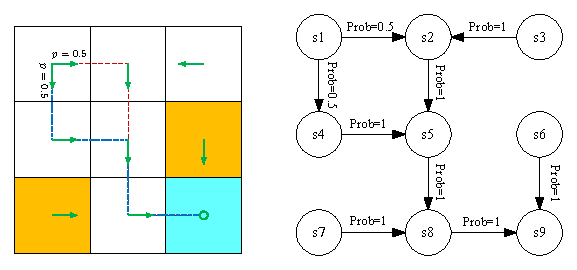
\includegraphics[width=277.1pt]{fig1_7}\par\smallskip
  \begin{minipage}{0.94\textwidth}\footnotesize
  \textbf{Figure 1.7.} Abstraction of the grid world example as a Markov process. Here, the circles represent states and the links with arrows represent state transitions.\par\smallskip
  \textcolor{rulegray}{\scriptsize Reproduced from S.~Zhao, \emph{Mathematical Foundations of Reinforcement Learning} (Springer, 2025).}
  \end{minipage}
\end{figure}


\subsection{Chapter 1 self-check}

\begin{enumerate}
  \item Why can adding $-2$ to every reward leave the optimal policy unchanged, but
        change every state value? \emph{(Answer: Theorem 3.6 and equation (3.8),
        \bkin{\S3.5, p.~51}.)}
  \item In the grid world, the agent bumps the wall at $s_1$ by taking $a_1$. What
        are $s'$, $r$, and $p(s_1\mid s_1,a_1)$? \emph{(Answer: $s'=s_1$,
        $r=-1$, probability $1$; \bkin{\S1.3, p.~3} and Table 1.3, p.~8.)}
  \item Write $G_t$ in terms of $G_{t+1}$ and explain in one sentence why this is
        the most important identity in the book.
  \item Why does the book insist that a return, not a reward, is the right thing to
        maximise? Give the two-policy numerical comparison from p.~8--9.
\end{enumerate}

\newpage
% ============================================================
\section{State Values and the Bellman Equation}
% ============================================================

\begin{roadmap}{Chapter 2 of the textbook}
\textbf{Textbook:} Chapter 2, ``State Values and Bellman Equation'', pp.~15--34.
Sections: \S2.1 why returns matter (p.~16), \S2.2 how to calculate returns (p.~17),
\S2.3 state values (p.~19), \S2.4 the Bellman equation (p.~20), \S2.5 worked
examples (p.~22), \S2.6 matrix--vector form (p.~25), \S2.7 solving for state values
(p.~27; closed form p.~27, iterative p.~28, examples p.~28), \S2.8 from state value
to action value (p.~30; examples p.~31; Bellman equation in action values p.~32),
\S2.9 summary (p.~33), \S2.10 Q\&A (p.~33).\\[0.3em]
\textbf{Videos:}
\vid{L2 P1 --- Motivating examples}{https://www.youtube.com/watch?v=XCzWrlgZCwc};
\vid{L2 P2 --- State value}{https://www.youtube.com/watch?v=DSvi3xEN13I};
\vid{L2 P3 --- Bellman equation derivation}{https://www.youtube.com/watch?v=eNtId8yPWkA};
\vid{L2 P4 --- Matrix--vector form and solution}{https://www.youtube.com/watch?v=EtCfBG_eP2w};
\vid{L2 P5 --- Action value}{https://www.youtube.com/watch?v=zJo2sLDzfcU}.\\[0.3em]
\textbf{What to take away:} the state value $v_\pi(s)=\E[G_t\mid S_t=s]$ is the
scoreboard for policies; the Bellman equation is a \emph{linear system} that
computes that scoreboard.
\end{roadmap}

\begin{figure}[htbp]
  \centering
  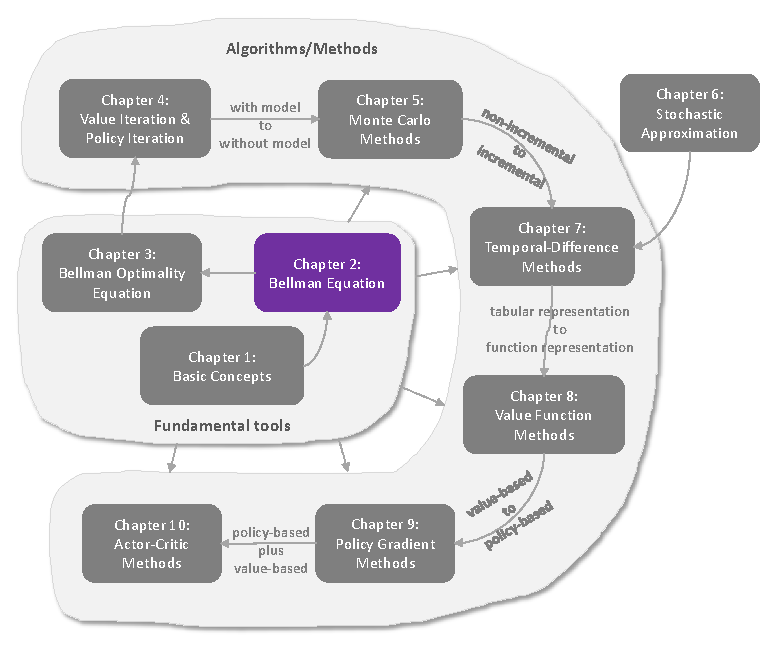
\includegraphics[width=371.3pt]{fig2_1}\par\smallskip
  \begin{minipage}{0.94\textwidth}\footnotesize
  \textbf{Figure 2.1.} Where we are in this book.\par\smallskip
  \textcolor{rulegray}{\scriptsize Reproduced from S.~Zhao, \emph{Mathematical Foundations of Reinforcement Learning} (Springer, 2025).}
  \end{minipage}
\end{figure}


\subsection{Motivating example 1: why returns are the right yardstick}

\bk{\S2.1, pp.~16--17; Figure 2.2, p.~16; inequality (2.1), p.~17}

The textbook opens with three policies that differ only at $s_1$ in a $2\times2$
grid (Figure 2.2, p.~16). $s_2$ is a forbidden cell, $s_4$ is the target.

\begin{worked}{ranking three policies by their returns \bkin{\S2.1, pp.~16--17}}
\textbf{Policy 1} (at $s_1$ go down). Trajectory
$s_1\to s_3\to s_4\to s_4\to\cdots$, with rewards $0,1,1,1,\dots$:
\[
  \text{return}_1 = 0 + \gamma 1 + \gamma^2 1 + \cdots
   = \gamma(1+\gamma+\gamma^2+\cdots)=\frac{\gamma}{1-\gamma}.
\]

\textbf{Policy 2} (at $s_1$ go right, into the forbidden cell). Trajectory
$s_1\to s_2\to s_4\to s_4\to\cdots$, rewards $-1,1,1,\dots$:
\[
  \text{return}_2 = -1+\gamma 1+\gamma^2 1+\cdots = -1+\frac{\gamma}{1-\gamma}.
\]

\textbf{Policy 3} (at $s_1$ go right or down, each with probability $0.5$).
Now there are two possible trajectories, each with probability $0.5$, so we average:
\[
  \text{return}_3 = 0.5\Bigl(-1+\frac{\gamma}{1-\gamma}\Bigr)
                  + 0.5\Bigl(\frac{\gamma}{1-\gamma}\Bigr)
                  = -0.5+\frac{\gamma}{1-\gamma}.
\]

\textbf{Conclusion.} For every $\gamma\in(0,1)$,
\[
  \text{return}_1 > \text{return}_3 > \text{return}_2,
\]
which is the book's inequality (2.1), p.~17. Policy 1 is best, policy 2 is worst,
and the stochastic policy 3 sits exactly in between. This matches the eyeball
verdict: policy 2 walks into the forbidden cell, policy 3 does so half the time.
\end{worked}

\begin{remark}
The book flags something important about $\text{return}_3$: it is not really a
return at all, because it averages over two different trajectories. It is an
\emph{expected} return. That object is precisely what we are about to name a
\textbf{state value} \bkin{\S2.1, p.~17}.
\end{remark}

\begin{figure}[htbp]
  \centering
  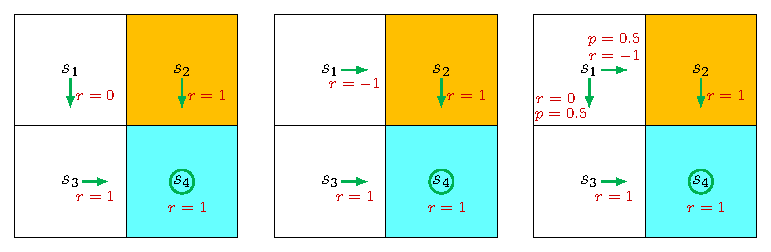
\includegraphics[width=370.2pt]{fig2_2}\par\smallskip
  \begin{minipage}{0.94\textwidth}\footnotesize
  \textbf{Figure 2.2.} Examples for demonstrating the importance of returns. The three examples have different policies for s1.\par\smallskip
  \textcolor{rulegray}{\scriptsize Reproduced from S.~Zhao, \emph{Mathematical Foundations of Reinforcement Learning} (Springer, 2025).}
  \end{minipage}
\end{figure}


\subsection{Motivating example 2: bootstrapping}

\bk{\S2.2, pp.~17--19; Figure 2.3, p.~18; equations (2.2)--(2.3)}

Consider a $2\times2$ grid in which the policy sends the agent round a cycle
$s_1\to s_2\to s_3\to s_4\to s_1\to\cdots$ collecting rewards $r_1,r_2,r_3,r_4$
along the way (the book's Figure 2.3, p.~18; there are no target or forbidden cells
here). Let $v_i$ be the return starting from $s_i$.

\textbf{Method A --- brute force} (the book's equation (2.2), p.~18):
\[
\begin{aligned}
  v_1 &= r_1+\gamma r_2+\gamma^2 r_3+\cdots,&\qquad
  v_2 &= r_2+\gamma r_3+\gamma^2 r_4+\cdots,\\
  v_3 &= r_3+\gamma r_4+\gamma^2 r_1+\cdots,&\qquad
  v_4 &= r_4+\gamma r_1+\gamma^2 r_2+\cdots.
\end{aligned}
\]

\textbf{Method B --- bootstrapping} (equation (2.3), p.~18). Factor out $\gamma$:
\[
  v_1 = r_1+\gamma v_2,\quad
  v_2 = r_2+\gamma v_3,\quad
  v_3 = r_3+\gamma v_4,\quad
  v_4 = r_4+\gamma v_1.
\]

\begin{intuition}
``Bootstrapping'' means computing something from itself. At first this looks like
circular reasoning: to get $v_1$ you need $v_2$, which needs $v_3$, which needs
$v_4$, which needs $v_1$. It is not circular --- it is a \emph{simultaneous system
of linear equations}, and you solve it the way you solved simultaneous equations in
high school. An economist should find this familiar: it is the same structure as a
Leontief input--output system $x=Ax+d$, or a linear rational-expectations model
where today's price depends on the expected price tomorrow.
\end{intuition}

Stack the four equations \bkin{\S2.2, p.~18}:
\[
  \underbrace{\begin{pmatrix}v_1\\v_2\\v_3\\v_4\end{pmatrix}}_{v}
  =\underbrace{\begin{pmatrix}r_1\\r_2\\r_3\\r_4\end{pmatrix}}_{r}
  +\gamma
  \underbrace{\begin{pmatrix}
    0&1&0&0\\ 0&0&1&0\\ 0&0&0&1\\ 1&0&0&0
  \end{pmatrix}}_{P}
  \begin{pmatrix}v_1\\v_2\\v_3\\v_4\end{pmatrix},
  \qquad\text{i.e.}\qquad v=r+\gamma Pv,
\]
whose solution is $v=(I-\gamma P)^{-1}r$. That $I-\gamma P$ is always invertible is
proved in \S2.7.1 (p.~27) and reproduced below.

\begin{figure}[htbp]
  \centering
  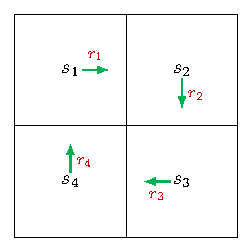
\includegraphics[width=121.2pt]{fig2_3}\par\smallskip
  \begin{minipage}{0.94\textwidth}\footnotesize
  \textbf{Figure 2.3.} An example for demonstrating how to calculate returns. There are no target or forbidden cells in this example.\par\smallskip
  \textcolor{rulegray}{\scriptsize Reproduced from S.~Zhao, \emph{Mathematical Foundations of Reinforcement Learning} (Springer, 2025).}
  \end{minipage}
\end{figure}


\subsection{State values}

\bk{\S2.3, pp.~19--20}

\begin{notation}
At time $t$ the agent is in state $S_t$, takes action $A_t$ under $\pi$, moves to
$S_{t+1}$ and collects $R_{t+1}$:
$S_t \xrightarrow{A_t} S_{t+1},R_{t+1}$. All four objects are random variables,
with $S_t,S_{t+1}\in\Sspace$, $A_t\in\Aspace(S_t)$, $R_{t+1}\in\mathcal{R}(S_t,A_t)$
\bkin{\S2.3, p.~19}.
\end{notation}

\begin{definition}[State value]
\[
  v_\pi(s) \;\doteq\; \E\bigl[G_t \mid S_t=s\bigr],
  \qquad
  G_t = R_{t+1}+\gamma R_{t+2}+\gamma^2 R_{t+3}+\cdots
\]
$v_\pi$ is called the \textbf{state-value function}, or simply the \textbf{state
value} of $s$ under $\pi$.
\end{definition}

Three properties the book emphasises \bkin{\S2.3, pp.~19--20}:

\begin{enumerate}
  \item $v_\pi(s)$ depends on $s$, because it is a \emph{conditional} expectation.
  \item $v_\pi(s)$ depends on $\pi$, because the trajectories are generated by $\pi$.
        Different policy, different number.
  \item $v_\pi(s)$ does \emph{not} depend on $t$. Once the policy and the
        (stationary) model are fixed, the number is determined.
\end{enumerate}

\begin{remark}[Return versus state value]
If both the policy and the model are deterministic, starting from $s$ always
produces the same trajectory, so the return equals the state value --- one number,
no averaging. If either is stochastic, different trajectories arise and the state
value is the \emph{mean} of their returns \bkin{\S2.3, p.~20}. This is why
$\text{return}_3$ in \S2.1 above was already secretly a state value.
\end{remark}

\textbf{The ranking rule.} $\pi_1$ is better than $\pi_2$ if
$v_{\pi_1}(s)\geq v_{\pi_2}(s)$ for \emph{all} $s\in\Sspace$. Note this is a
partial order: two policies can be incomparable if each is better at some states.
Chapter 3 shows, remarkably, that a policy exists which dominates \emph{every}
other policy at \emph{every} state simultaneously \bkin{Definition 3.1, \S3.2, p.~38}.

\subsection{The Bellman equation}

\bk{\S2.4, pp.~20--22; equations (2.4)--(2.7)}
\ \vid{L2 P3 --- derivation}{https://www.youtube.com/watch?v=eNtId8yPWkA}

Start from the bootstrapping identity $G_t=R_{t+1}+\gamma G_{t+1}$ and take
conditional expectations \bkin{equation (2.4), p.~20}:
\[
  v_\pi(s)=\E[G_t\mid S_t=s]
  =\E[R_{t+1}\mid S_t=s]+\gamma\,\E[G_{t+1}\mid S_t=s].
\]
Now expand each piece.

\paragraph{The immediate-reward term.} By the law of total expectation
\bkin{equation (2.5), p.~21}:
\[
  \E[R_{t+1}\mid S_t=s]
  =\sum_{a\in\Aspace}\pi(a\mid s)\,\E[R_{t+1}\mid S_t=s,A_t=a]
  =\sum_{a\in\Aspace}\pi(a\mid s)\sum_{r\in\mathcal R}p(r\mid s,a)\,r.
\]
Read it right to left: given the action, average over rewards; then average over
actions using the policy.

\paragraph{The future-reward term.} \bkin{equation (2.6), p.~21}
\[
\begin{aligned}
  \E[G_{t+1}\mid S_t=s]
  &=\sum_{s'\in\Sspace}\E[G_{t+1}\mid S_t=s,S_{t+1}=s']\,p(s'\mid s)\\
  &=\sum_{s'\in\Sspace}\E[G_{t+1}\mid S_{t+1}=s']\,p(s'\mid s)
    &&\text{(Markov property)}\\
  &=\sum_{s'\in\Sspace}v_\pi(s')\,p(s'\mid s)
   =\sum_{s'\in\Sspace}v_\pi(s')\sum_{a\in\Aspace}p(s'\mid s,a)\pi(a\mid s).
\end{aligned}
\]
The second line is the \emph{only} place the Markov property is used: knowing you
arrived at $s'$ makes the route you took irrelevant.

\paragraph{Putting them together.}

\begin{definition}[Bellman equation, textbook equation (2.7), p.~21]
\[
  \boxed{\;
  v_\pi(s)=\sum_{a\in\Aspace}\pi(a\mid s)
  \Bigl[\underbrace{\sum_{r\in\mathcal R}p(r\mid s,a)\,r}_{\text{mean immediate reward}}
       +\gamma\underbrace{\sum_{s'\in\Sspace}p(s'\mid s,a)\,v_\pi(s')}_{\text{mean future reward}}\Bigr],
  \quad \forall s\in\Sspace. \;}
\]
\end{definition}

Four things to notice \bkin{\S2.4, p.~22}:

\begin{itemize}
  \item $v_\pi(s)$ and $v_\pi(s')$ are the \textbf{unknowns}. It is not one
        equation --- it is $|\Sspace|$ equations, one per state, and they are
        \emph{linear} in the unknowns.
  \item $\pi(a\mid s)$ is \textbf{given}. Solving the system for a given $\pi$ is
        called \textbf{policy evaluation}, and it is a subroutine inside almost
        every algorithm in the rest of the book.
  \item $p(r\mid s,a)$ and $p(s'\mid s,a)$ are the \textbf{model}. Chapters 5--10
        are about what to do when you do not have them.
  \item Two equivalent forms appear in the literature \bkin{\S2.4, p.~22}:
        $v_\pi(s)=\sum_a\pi(a\mid s)\sum_{s'}\sum_r p(s',r\mid s,a)[r+\gamma v_\pi(s')]$
        (used by Sutton \& Barto), and, when the reward depends only on the next
        state, $v_\pi(s)=\sum_a\pi(a\mid s)\sum_{s'}p(s'\mid s,a)[r(s')+\gamma v_\pi(s')]$.
\end{itemize}

\subsection{Two fully worked Bellman examples}

\bk{\S2.5, pp.~22--25; Figures 2.4--2.5}

\begin{worked}{a deterministic policy \bkin{Figure 2.4, p.~23}}
$2\times2$ grid, $s_2$ forbidden, $s_4$ target, $\gamma=0.9$. The policy sends
$s_1$ down, $s_2$ down, $s_3$ right, and $s_4$ stays.

\textbf{Step 1: state $s_1$.} Under this policy $\pi(a_3\mid s_1)=1$ and
$\pi(a\neq a_3\mid s_1)=0$. Transitions: $p(s_3\mid s_1,a_3)=1$. Rewards:
$p(r=0\mid s_1,a_3)=1$. Substituting into (2.7) collapses the triple sum to a
single term:
\[
  v_\pi(s_1)=0+\gamma v_\pi(s_3).
\]
Note how a formidable-looking formula becomes trivial once the policy and model are
deterministic --- this is exactly the book's point.

\textbf{Step 2: the other states.}
\[
  v_\pi(s_2)=1+\gamma v_\pi(s_4),\qquad
  v_\pi(s_3)=1+\gamma v_\pi(s_4),\qquad
  v_\pi(s_4)=1+\gamma v_\pi(s_4).
\]

\textbf{Step 3: solve.} The last equation gives $v_\pi(s_4)=1/(1-\gamma)$ and the
rest follow by back-substitution:
\[
  v_\pi(s_4)=v_\pi(s_3)=v_\pi(s_2)=\frac{1}{1-\gamma},
  \qquad v_\pi(s_1)=\frac{\gamma}{1-\gamma}.
\]

\textbf{Step 4: put in $\gamma=0.9$.}
\[
  v_\pi(s_4)=v_\pi(s_3)=v_\pi(s_2)=\frac{1}{0.1}=10,
  \qquad v_\pi(s_1)=\frac{0.9}{0.1}=9.
\]
\end{worked}

\begin{worked}{a stochastic policy \bkin{Figure 2.5, p.~24}}
Same grid, but at $s_1$ the agent goes right or down with probability $0.5$ each:
$\pi(a_2\mid s_1)=\pi(a_3\mid s_1)=0.5$. Going right lands on the forbidden cell
$s_2$ and earns $r=-1$; going down lands on $s_3$ and earns $r=0$.

The Bellman equation at $s_1$ now has two terms:
\[
  v_\pi(s_1)=0.5\bigl[0+\gamma v_\pi(s_3)\bigr]+0.5\bigl[-1+\gamma v_\pi(s_2)\bigr].
\]
The other three states are unchanged, so again
$v_\pi(s_2)=v_\pi(s_3)=v_\pi(s_4)=1/(1-\gamma)$ and
\[
  v_\pi(s_1)=-0.5+\frac{\gamma}{1-\gamma}.
\]
With $\gamma=0.9$: $v_\pi(s_2)=v_\pi(s_3)=v_\pi(s_4)=10$ and
$v_\pi(s_1)=-0.5+9=8.5$.

\textbf{Comparison.} $9 > 8.5$, and the two policies tie everywhere else, so
$v_{\pi_1}(s_i)\geq v_{\pi_2}(s_i)$ for all $i$: the deterministic policy is better
\bkin{\S2.5, p.~25}. State values have delivered a verdict that agrees with
intuition, and they did so by arithmetic rather than by inspection.
\end{worked}

\begin{figure}[htbp]
  \centering
  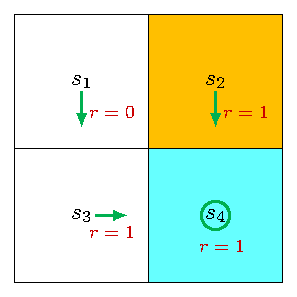
\includegraphics[width=142.6pt]{fig2_4}\par\smallskip
  \begin{minipage}{0.94\textwidth}\footnotesize
  \textbf{Figure 2.4.} An example for demonstrating the Bellman equation. The policy in this example is deter- ministic.\par\smallskip
  \textcolor{rulegray}{\scriptsize Reproduced from S.~Zhao, \emph{Mathematical Foundations of Reinforcement Learning} (Springer, 2025).}
  \end{minipage}
\end{figure}


\begin{figure}[htbp]
  \centering
  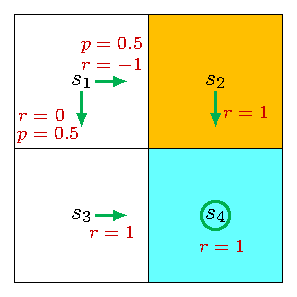
\includegraphics[width=142.6pt]{fig2_5}\par\smallskip
  \begin{minipage}{0.94\textwidth}\footnotesize
  \textbf{Figure 2.5.} An example for demonstrating the Bellman equation. The policy in this example is stochastic.\par\smallskip
  \textcolor{rulegray}{\scriptsize Reproduced from S.~Zhao, \emph{Mathematical Foundations of Reinforcement Learning} (Springer, 2025).}
  \end{minipage}
\end{figure}


\subsection{Matrix--vector form}

\bk{\S2.6, pp.~25--27; equations (2.8)--(2.10)}
\ \vid{L2 P4}{https://www.youtube.com/watch?v=EtCfBG_eP2w}

Define, for each state, the policy-averaged reward and the policy-induced
transition probability \bkin{\S2.6, p.~26}:
\[
  r_\pi(s)\doteq\sum_{a}\pi(a\mid s)\sum_{r}p(r\mid s,a)\,r,
  \qquad
  p_\pi(s'\mid s)\doteq\sum_{a}\pi(a\mid s)\,p(s'\mid s,a).
\]
Then the Bellman equation (2.7) becomes
$v_\pi(s)=r_\pi(s)+\gamma\sum_{s'}p_\pi(s'\mid s)v_\pi(s')$ \bkin{equation (2.8)},
and stacking over $s_1,\dots,s_n$ with $n=|\Sspace|$:

\begin{definition}[Matrix--vector Bellman equation, equation (2.10), p.~26]
\[
  \boxed{\;v_\pi = r_\pi + \gamma P_\pi v_\pi\;}
\]
where $v_\pi,r_\pi\in\R^n$ and $[P_\pi]_{ij}=p_\pi(s_j\mid s_i)$.
\end{definition}

\begin{fact}[Properties of $P_\pi$, \bkin{\S2.6, p.~26}]
$P_\pi\ge 0$ elementwise, and $P_\pi$ is a \textbf{stochastic matrix}: every row
sums to one, i.e.\ $P_\pi\mathbf{1}=\mathbf{1}$.
\end{fact}

\begin{worked}{the matrix form of the stochastic example \bkin{Figure 2.6, p.~27}}
For the four-state example with $\pi(a_2\mid s_1)=\pi(a_3\mid s_1)=0.5$:
\[
  \begin{pmatrix}v_\pi(s_1)\\v_\pi(s_2)\\v_\pi(s_3)\\v_\pi(s_4)\end{pmatrix}
  =\begin{pmatrix}0.5(0)+0.5(-1)\\1\\1\\1\end{pmatrix}
  +\gamma\begin{pmatrix}
    0&0.5&0.5&0\\
    0&0&0&1\\
    0&0&0&1\\
    0&0&0&1
  \end{pmatrix}
  \begin{pmatrix}v_\pi(s_1)\\v_\pi(s_2)\\v_\pi(s_3)\\v_\pi(s_4)\end{pmatrix}.
\]
Every row of $P_\pi$ sums to $1$, as promised. Row 1 reads: from $s_1$, go to $s_2$
with probability $0.5$ and to $s_3$ with probability $0.5$.
\end{worked}

\begin{figure}[htbp]
  \centering
  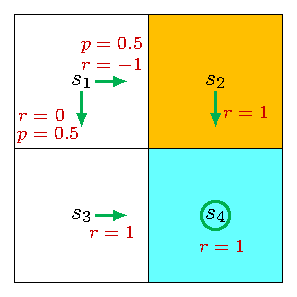
\includegraphics[width=142.6pt]{fig2_6}\par\smallskip
  \begin{minipage}{0.94\textwidth}\footnotesize
  \textbf{Figure 2.6.} An example for demonstrating the matrix-vector form of the Bellman equation.\par\smallskip
  \textcolor{rulegray}{\scriptsize Reproduced from S.~Zhao, \emph{Mathematical Foundations of Reinforcement Learning} (Springer, 2025).}
  \end{minipage}
\end{figure}


\subsection{Solving for state values}

\bk{\S2.7, pp.~27--30}

\subsubsection{Method 1: closed form}

\bk{\S2.7.1, p.~27}

\[
  v_\pi=(I-\gamma P_\pi)^{-1}r_\pi.
\]

\begin{theorem}[Invertibility]
$I-\gamma P_\pi$ is invertible for every $\gamma\in(0,1)$ and every policy $\pi$.
\end{theorem}

\begin{proof}[Proof sketch (the book's argument, p.~27)]
Use the Gershgorin circle theorem: every eigenvalue lies in at least one disc
centred at a diagonal entry $[I-\gamma P_\pi]_{ii}=1-\gamma p_\pi(s_i\mid s_i)$ with
radius $\sum_{j\neq i}\gamma p_\pi(s_j\mid s_i)$. Because rows of $P_\pi$ sum to one
and $\gamma<1$,
\[
  \sum_{j\ne i}\gamma p_\pi(s_j\mid s_i)
  = \gamma\bigl(1-p_\pi(s_i\mid s_i)\bigr)
  < 1-\gamma p_\pi(s_i\mid s_i),
\]
so no disc contains the origin, so no eigenvalue is zero.
\end{proof}

Two further properties the book records \bkin{\S2.7.1, p.~27}, both useful later:
\begin{itemize}
  \item $(I-\gamma P_\pi)^{-1}=I+\gamma P_\pi+\gamma^2P_\pi^2+\cdots\ \ge\ I\ \ge 0$
        (a Neumann series with nonnegative terms).
  \item If $r\ge 0$ then $(I-\gamma P_\pi)^{-1}r\ge r\ge 0$; and if $r_1\ge r_2$
        then $(I-\gamma P_\pi)^{-1}r_1\ge(I-\gamma P_\pi)^{-1}r_2$. Monotonicity of
        this operator is what makes ``a better reward gives a better value'' true.
\end{itemize}

\begin{warning}
The closed form is a theoretical device, not an algorithm. Inverting an
$n\times n$ matrix costs $O(n^3)$, and real problems have $n$ in the millions.
The book says so explicitly \bkin{\S2.7.2, p.~28}.
\end{warning}

\subsubsection{Method 2: iteration}

\bk{\S2.7.2, p.~28; equations (2.11)--(2.12); Box 2.1, p.~28}

Pick any $v_0\in\R^n$ and iterate
\[
  v_{k+1}=r_\pi+\gamma P_\pi v_k,\qquad k=0,1,2,\dots
\]
Then $v_k\to v_\pi=(I-\gamma P_\pi)^{-1}r_\pi$ as $k\to\infty$.

\begin{proof}[Convergence proof (the book's Box 2.1, p.~28)]
Let $\delta_k=v_k-v_\pi$. Substituting $v_k=\delta_k+v_\pi$ into the iteration and
using $v_\pi=r_\pi+\gamma P_\pi v_\pi$,
\[
  \delta_{k+1}+v_\pi = r_\pi+\gamma P_\pi(\delta_k+v_\pi)
  \;\Longrightarrow\;
  \delta_{k+1}=\gamma P_\pi\delta_k = \cdots = \gamma^{k+1}P_\pi^{k+1}\delta_0 .
\]
Every entry of $P_\pi^k$ lies in $[0,1]$ for all $k$ (products of stochastic
matrices are stochastic), while $\gamma^{k}\to0$. Hence $\delta_k\to0$.
\end{proof}

\begin{intuition}
The error shrinks by a factor of at least $\gamma$ every sweep. With $\gamma=0.9$
you lose one digit of error roughly every $22$ iterations
($0.9^{22}\approx0.10$); with $\gamma=0.5$, every $3.3$ iterations. Small $\gamma$
means fast convergence but a short-sighted agent --- the first of many
discount-rate trade-offs.
\end{intuition}

\subsubsection{What state values look like}

\bk{\S2.7.3, pp.~28--30; Figure 2.7, p.~29}

The book applies the iteration to a $5\times5$ grid with
$r_{\text{boundary}}=r_{\text{forbidden}}=-1$, $r_{\text{target}}=1$, $\gamma=0.9$,
and shows four policies (Figure 2.7, p.~29). Two lessons:

\begin{itemize}
  \item \textbf{Good policies have large values.} The two ``good'' policies both
        produce the value grid whose row~1 reads
        $3.5,\ 3.9,\ 4.3,\ 4.8,\ 5.3$ and whose target cell holds $10.0$
        \bkin{Figure 2.7(a), p.~29}.
  \item \textbf{Different policies can share the same state values.} The two good
        policies in Figure 2.7(a) differ at the top two states of column 4 yet have
        identical values. \emph{Values do not determine the policy uniquely.} This
        prefigures the non-uniqueness of optimal policies in Chapter 3
        \bkin{\S3.4, p.~48}.
  \item \textbf{Bad policies have small, often negative values.} The ``bad''
        policies in Figure 2.7(b) produce values like $-6.6,-7.3,-8.1,-9.0,-10.0$
        across row~1.
\end{itemize}

\begin{figure}[htbp]
  \centering
  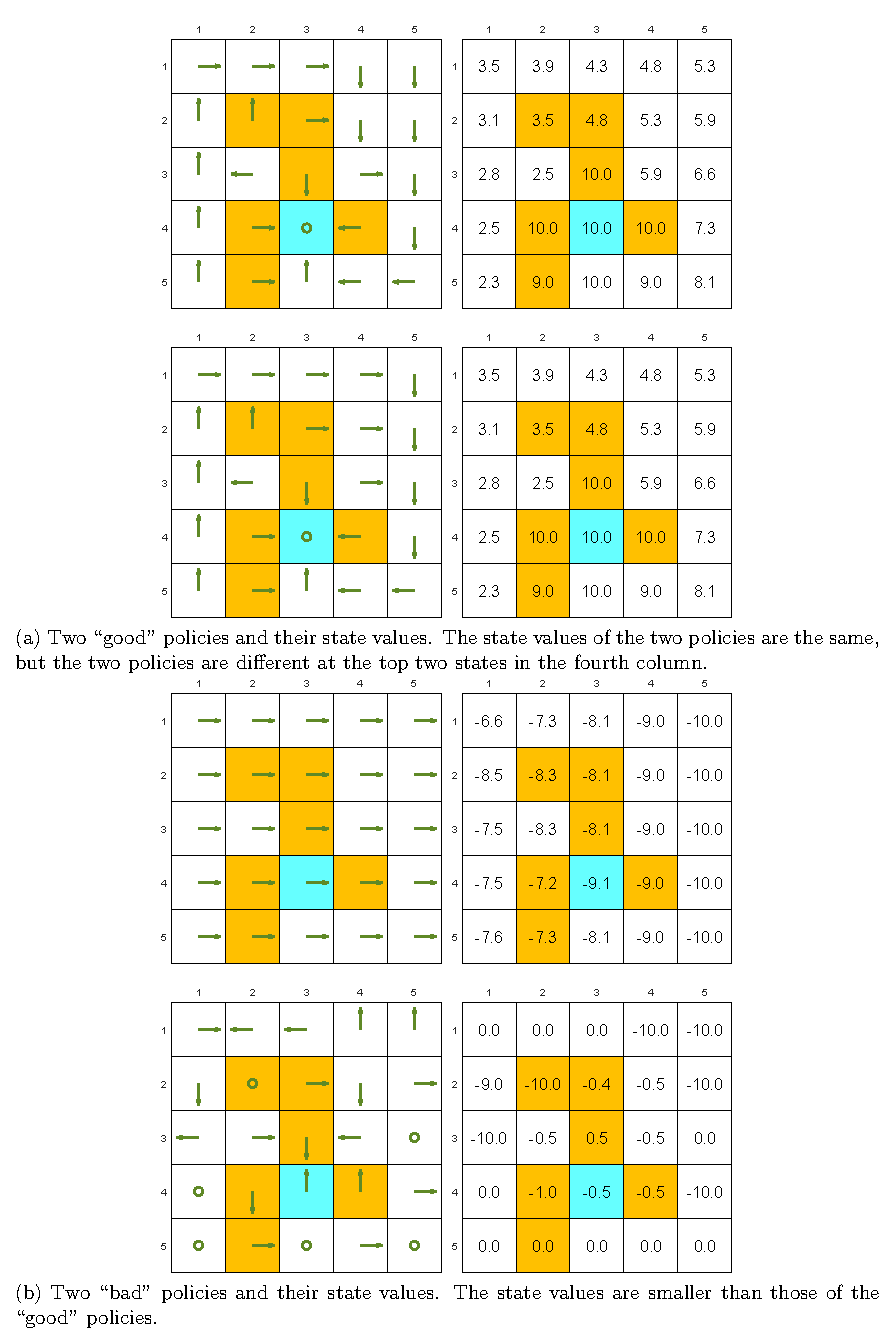
\includegraphics[width=268.0pt]{fig2_7}\par\smallskip
  \begin{minipage}{0.94\textwidth}\footnotesize
  \textbf{Figure 2.7.} Examples of policies and their corresponding state values.\par\smallskip
  \textcolor{rulegray}{\scriptsize Reproduced from S.~Zhao, \emph{Mathematical Foundations of Reinforcement Learning} (Springer, 2025).}
  \end{minipage}
\end{figure}


\subsection{From state values to action values}

\bk{\S2.8, pp.~30--33}
\ \vid{L2 P5}{https://www.youtube.com/watch?v=zJo2sLDzfcU}

\begin{definition}[Action value]
\[
  q_\pi(s,a)\;\doteq\;\E[G_t\mid S_t=s,\ A_t=a].
\]
It is the expected return from \emph{committing} to action $a$ at $s$ and following
$\pi$ forever after. Strictly it should be called a state--action value; everyone
says ``action value'' or ``$Q$-value''.
\end{definition}

Two identities link $v$ and $q$ --- the book calls them ``two sides of the same
coin'' \bkin{\S2.8, p.~31}.

\begin{theorem}[The $v$--$q$ relations, equations (2.13)--(2.14), pp.~30--31]
\[
  \text{(2.13)}\quad v_\pi(s)=\sum_{a\in\Aspace}\pi(a\mid s)\,q_\pi(s,a),
\]
\[
  \text{(2.14)}\quad q_\pi(s,a)=\sum_{r\in\mathcal R}p(r\mid s,a)\,r
    +\gamma\sum_{s'\in\Sspace}p(s'\mid s,a)\,v_\pi(s').
\]
\end{theorem}

Equation (2.13) says a state value is the policy-weighted average of that state's
action values. Equation (2.14) says an action value is the mean immediate reward
plus the discounted mean of the \emph{next} states' values. Substituting (2.14)
into (2.13) recovers the Bellman equation --- which is a good consistency check.

\begin{worked}{action values at $s_1$, and a mistake to avoid \bkin{\S2.8.1, pp.~31--32; Figure 2.8}}
Take the stochastic policy of Figure 2.8 (p.~31): at $s_1$ the agent goes right
($a_2$, into forbidden $s_2$, $r=-1$) or down ($a_3$, into $s_3$, $r=0$), each with
probability $0.5$. The values computed earlier were $v_\pi(s_1)=8.5$,
$v_\pi(s_2)=v_\pi(s_3)=v_\pi(s_4)=10$, $\gamma=0.9$.

\textbf{The two actions the policy does take:}
\[
  q_\pi(s_1,a_2)=-1+\gamma v_\pi(s_2)=-1+9=8,
  \qquad
  q_\pi(s_1,a_3)=0+\gamma v_\pi(s_3)=9.
\]

\textbf{The three actions the policy never takes.} A beginner might set these to
zero, or refuse to compute them. \emph{Both are wrong} \bkin{\S2.8.1, p.~31}. They
are perfectly well defined: take the action once, then follow $\pi$ afterwards.
At $s_1$, actions $a_1$ (up) and $a_4$ (left) bounce off the wall, so the agent
returns to $s_1$ with $r=-1$; action $a_5$ stays at $s_1$ with $r=0$:
\[
  q_\pi(s_1,a_1)=-1+\gamma v_\pi(s_1)=-1+0.9(8.5)=6.65,
\]
\[
  q_\pi(s_1,a_4)=-1+\gamma v_\pi(s_1)=6.65,
  \qquad
  q_\pi(s_1,a_5)=0+\gamma v_\pi(s_1)=7.65 .
\]

\textbf{Consistency check via (2.13):}
\[
  v_\pi(s_1)=0.5\,q_\pi(s_1,a_2)+0.5\,q_\pi(s_1,a_3)=0.5(8)+0.5(9)=8.5.\ \checkmark
\]
\end{worked}

\begin{warning}[Why we care about actions the policy will not take]
This is the single most important remark in Chapter 2 and the reason the whole
book works \bkin{\S2.8.1, p.~32; \S2.10 Q\&A, p.~34}. If a policy never selects
action $a$ at $s$, that is not evidence that $a$ is bad --- it may be evidence that
the \emph{policy} is bad and is missing the best action. In this very example,
$q_\pi(s_1,a_3)=9$ is the largest of the five, so a better policy would put all its
probability on $a_3$. \textbf{Policy improvement is nothing but comparing action
values, including the ones you are not currently using.} That is why exploration
matters (Chapter 5) and why model-free methods estimate $q$ rather than $v$
(Chapter 5, \S5.2.1, p.~80).
\end{warning}

\begin{figure}[htbp]
  \centering
  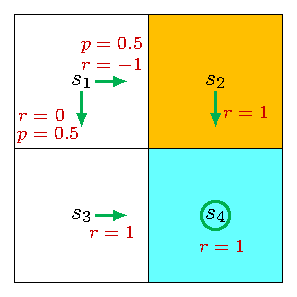
\includegraphics[width=142.6pt]{fig2_8}\par\smallskip
  \begin{minipage}{0.94\textwidth}\footnotesize
  \textbf{Figure 2.8.} An example for demonstrating the process of calculating action values.\par\smallskip
  \textcolor{rulegray}{\scriptsize Reproduced from S.~Zhao, \emph{Mathematical Foundations of Reinforcement Learning} (Springer, 2025).}
  \end{minipage}
\end{figure}


\subsubsection{The Bellman equation in action values}

\bk{\S2.8.2, pp.~32--33; equation (2.15)}

Substituting (2.13) into (2.14) eliminates $v$ entirely:
\[
  q_\pi(s,a)=\sum_{r}p(r\mid s,a)\,r
    +\gamma\sum_{s'}p(s'\mid s,a)\sum_{a'\in\Aspace(s')}\pi(a'\mid s')\,q_\pi(s',a').
\]
In matrix form \bkin{equation (2.15), p.~32}: $q_\pi=\tilde r+\gamma P\Pi q_\pi$,
where $q_\pi$ and $\tilde r$ are indexed by state--action pairs,
$[P]_{(s,a),s'}=p(s'\mid s,a)$, and $\Pi$ is block diagonal with
$\Pi_{s',(s',a')}=\pi(a'\mid s')$.

\begin{remark}
This version has a feature that matters in Chapters 7--8: $\tilde r$ and $P$ depend
only on the \emph{environment}, and the policy is quarantined inside $\Pi$. This
separation is what makes off-policy learning conceivable \bkin{\S2.8.2, p.~33}.
\end{remark}

\subsection{Chapter 2 self-check}

\begin{enumerate}
  \item State the Bellman equation from memory, then say in words what each of the
        four sums is averaging over.
  \item Where exactly in the derivation is the Markov property used, and what would
        break without it? \emph{(Answer: equation (2.6), p.~21.)}
  \item In the $\gamma=0.9$ stochastic example, verify by hand that
        $v_\pi(s_1)=8.5$ satisfies its own Bellman equation.
  \item Two policies have identical state values everywhere. Must they be the same
        policy? \emph{(No --- Figure 2.7(a), p.~29.)}
  \item Why must a model-free algorithm estimate $q_\pi$ rather than $v_\pi$?
        \emph{(Look at (2.14): converting $v$ to $q$ needs $p(r\mid s,a)$ and
        $p(s'\mid s,a)$; \bkin{\S5.2.1, p.~81}.)}
\end{enumerate}

\newpage
% ============================================================
\section{Optimal State Values and the Bellman Optimality Equation}
% ============================================================

\begin{roadmap}{Chapter 3 of the textbook}
\textbf{Textbook:} Chapter 3, pp.~35--55. Sections: \S3.1 motivating example ---
how to improve policies (p.~36), \S3.2 optimal state values and optimal policies
(p.~37), \S3.3 the Bellman optimality equation (p.~38; maximisation of the RHS
p.~39, matrix--vector form p.~40, contraction mapping theorem p.~40, contraction
property of the RHS p.~44), \S3.4 solving an optimal policy from the BOE (p.~46),
\S3.5 factors that influence optimal policies (p.~49), \S3.6 summary (p.~53),
\S3.7 Q\&A (p.~54).\\[0.3em]
\textbf{Videos:}
\vid{L3 P1 --- Motivating example}{https://www.youtube.com/watch?v=lXKY_Hyg4SQ};
\vid{L3 P2 --- Optimal policy}{https://www.youtube.com/watch?v=BxyjdHhK8a8};
\vid{L3 P3 --- More on the BOE}{https://www.youtube.com/watch?v=FXftTCKotC8};
\vid{L3 P4 --- Interesting properties}{https://www.youtube.com/watch?v=a--bck2ow9s}.\\[0.3em]
\textbf{Warning from the author:} this is the most mathematically intensive chapter
of the first half, and it is worth it, because it answers the four questions ---
does an optimal policy exist, is it unique, is it stochastic, how do we find it
\bkin{\S3.2, p.~38}.
\end{roadmap}

\begin{figure}[htbp]
  \centering
  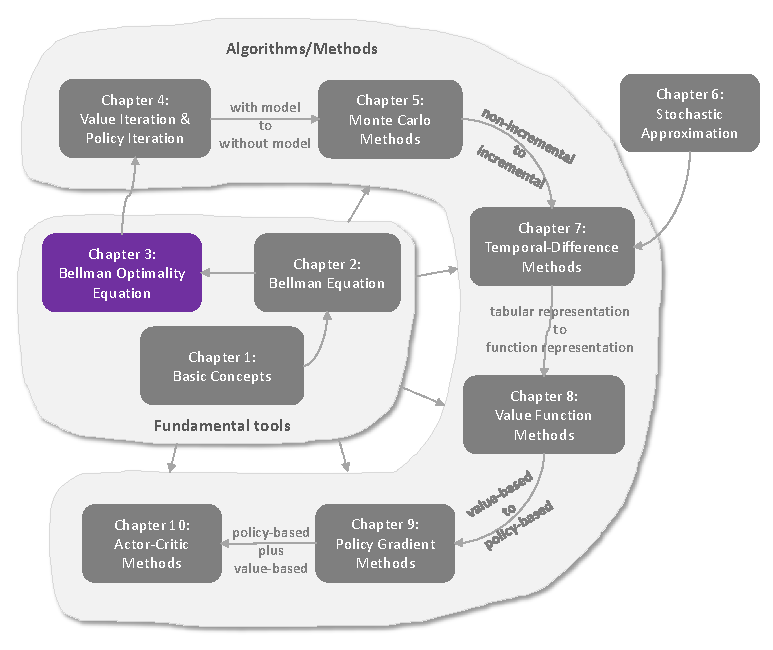
\includegraphics[width=371.3pt]{fig3_1}\par\smallskip
  \begin{minipage}{0.94\textwidth}\footnotesize
  \textbf{Figure 3.1.} Where we are in this book.\par\smallskip
  \textcolor{rulegray}{\scriptsize Reproduced from S.~Zhao, \emph{Mathematical Foundations of Reinforcement Learning} (Springer, 2025).}
  \end{minipage}
\end{figure}


\subsection{Motivating example: how do you improve a policy?}

\bk{\S3.1, pp.~36--37; Figure 3.2, p.~36}

Take the $2\times2$ grid ($s_2$ forbidden, $s_4$ target, $\gamma=0.9$) with a
policy that stupidly sends the agent \emph{right} at $s_1$, straight into the
forbidden cell. Can we fix it, and can we justify the fix with arithmetic rather
than with eyeballs?

\begin{worked}{one step of policy improvement \bkin{\S3.1, pp.~36--37}}
\textbf{Step 1 --- evaluate the current policy.} Its Bellman equations are
\[
  v_\pi(s_1)=-1+\gamma v_\pi(s_2),\quad
  v_\pi(s_2)=+1+\gamma v_\pi(s_4),\quad
  v_\pi(s_3)=+1+\gamma v_\pi(s_4),\quad
  v_\pi(s_4)=+1+\gamma v_\pi(s_4).
\]
With $\gamma=0.9$: $v_\pi(s_4)=v_\pi(s_3)=v_\pi(s_2)=10$ and
$v_\pi(s_1)=-1+9=8$.

\textbf{Step 2 --- compute all five action values at $s_1$} using (2.14):
\[
\begin{aligned}
  q_\pi(s_1,a_1)&=-1+\gamma v_\pi(s_1)=-1+7.2=6.2 &&\text{(up: bounces off wall)}\\
  q_\pi(s_1,a_2)&=-1+\gamma v_\pi(s_2)=-1+9=8     &&\text{(right: into forbidden cell)}\\
  q_\pi(s_1,a_3)&=\phantom{-}0+\gamma v_\pi(s_3)=9 &&\text{(down: the good move)}\\
  q_\pi(s_1,a_4)&=-1+\gamma v_\pi(s_1)=6.2         &&\text{(left: bounces off wall)}\\
  q_\pi(s_1,a_5)&=\phantom{-}0+\gamma v_\pi(s_1)=7.2 &&\text{(stay)}
\end{aligned}
\]

\textbf{Step 3 --- act greedily.} $q_\pi(s_1,a_3)=9$ is the largest, so set
$\pi_{\text{new}}(a_3\mid s_1)=1$. The new policy avoids the forbidden cell.
\end{worked}

\begin{intuition}
This three-line recipe --- evaluate, compute $q$, take the argmax --- is the
skeleton of \emph{every} algorithm in Chapters 4, 5, 7 and 8. What changes across
chapters is only \emph{how} you get the $q$ values: by solving equations
(Chapter 4), by averaging sampled returns (Chapter 5), by one-step bootstrapped
updates (Chapter 7), or by fitting a function (Chapter 8).
\end{intuition}

The example leaves open the hard questions: what if the policy is bad at
\emph{many} states? Does greedy improvement always work? Does an optimal policy
even exist? Chapter 3 answers all of them.

\begin{figure}[htbp]
  \centering
  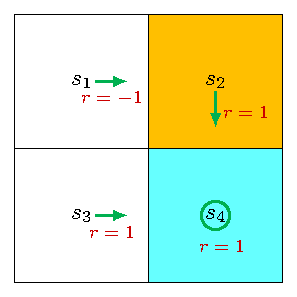
\includegraphics[width=142.6pt]{fig3_2}\par\smallskip
  \begin{minipage}{0.94\textwidth}\footnotesize
  \textbf{Figure 3.2.} An example for demonstrating policy improvement.\par\smallskip
  \textcolor{rulegray}{\scriptsize Reproduced from S.~Zhao, \emph{Mathematical Foundations of Reinforcement Learning} (Springer, 2025).}
  \end{minipage}
\end{figure}


\subsection{Defining optimality}

\bk{\S3.2, pp.~37--38; Definition 3.1, p.~38}

\begin{definition}[Optimal policy and optimal state value, Definition 3.1, p.~38]
A policy $\pi^*$ is \textbf{optimal} if
\[
  v_{\pi^*}(s)\ \ge\ v_\pi(s)\qquad\text{for all }s\in\Sspace
  \text{ and for every other policy }\pi .
\]
Its state values $v^*=v_{\pi^*}$ are the \textbf{optimal state values}.
\end{definition}

\begin{warning}
Read the quantifiers carefully. This is a very strong demand: $\pi^*$ must beat
every rival at \emph{every state simultaneously}. Nothing in the definition
guarantees such a policy exists --- \emph{a priori} you would expect trade-offs,
where policy $A$ is better at some states and policy $B$ at others. The content of
Chapter 3 is that for finite discounted MDPs no such trade-off arises. That is a
genuinely surprising theorem, not a definition.
\end{warning}

\begin{remark}
The book also flags a scope limitation \bkin{\S3.7 Q\&A, p.~54}: this definition of
optimality is valid for \emph{tabular} RL. Once values or policies are
approximated by functions (Chapters 8--9), you cannot achieve the maximum at every
state at once, and optimality must be redefined via a scalar objective
\bkin{\S9.2, p.~193}.
\end{remark}

\subsection{The Bellman optimality equation}

\bk{\S3.3, pp.~38--39; equation (3.1), p.~38}

\begin{definition}[BOE, elementwise, equation (3.1), p.~38]
For every $s\in\Sspace$,
\[
  \boxed{\;
  v(s)=\max_{\pi(s)\in\Pi(s)}\sum_{a\in\Aspace}\pi(a\mid s)
  \Bigl[\sum_{r}p(r\mid s,a)\,r+\gamma\sum_{s'}p(s'\mid s,a)\,v(s')\Bigr]
  =\max_{\pi(s)\in\Pi(s)}\sum_{a}\pi(a\mid s)\,q(s,a),
  \;}
\]
where $q(s,a)\doteq\sum_r p(r\mid s,a)r+\gamma\sum_{s'}p(s'\mid s,a)v(s')$.
\end{definition}

Compare with the ordinary Bellman equation: the policy-weighted average
$\sum_a\pi(a\mid s)(\cdot)$ has become a \emph{maximisation over policies}. That
one change makes the equation \textbf{nonlinear} --- you can no longer invert a
matrix --- and introduces a second unknown: both $v(s)$ and $\pi$ are unknown.

\subsubsection{Solving the maximisation on the right-hand side}

\bk{\S3.3.1, pp.~39--40; Examples 3.1--3.2}

\begin{worked}{Example 3.1, p.~39 --- two unknowns, one equation}
Solve $x=\max_{y\in\R}(2x-1-y^2)$ for $x,y\in\R$.

\emph{Step 1: eliminate $y$.} Whatever $x$ is, $\max_y(2x-1-y^2)=2x-1$, attained at
$y=0$.

\emph{Step 2: now solve $x$.} The equation becomes $x=2x-1$, so $x=1$.

\emph{Answer:} $y=0$, $x=1$. Two unknowns, one equation --- solved by doing the
inner optimisation first. \textbf{The BOE is solved the same way.}
\end{worked}

\begin{worked}{Example 3.2, p.~39 --- how to maximise a weighted average}
Given fixed numbers $q_1,q_2,q_3$, choose weights $c_1,c_2,c_3\ge0$ with
$c_1+c_2+c_3=1$ to maximise $\sum_i c_iq_i$.

Suppose $q_3\ge q_1,q_2$. Then
\[
  q_3=(c_1+c_2+c_3)q_3=c_1q_3+c_2q_3+c_3q_3\ \ge\ c_1q_1+c_2q_2+c_3q_3
\]
for any admissible weights. So the maximum is $q_3$, attained at $c_3^*=1$,
$c_1^*=c_2^*=0$.

\textbf{Moral:} to maximise a weighted average, put all the weight on the largest
item. Not half on the largest and half on the second largest --- \emph{all} of it.
\end{worked}

Applying Example 3.2 with $c_a=\pi(a\mid s)$ and $q_a=q(s,a)$ \bkin{\S3.3.1, p.~40}:
\[
  \sum_{a}\pi(a\mid s)q(s,a)\ \le\ \max_{a\in\Aspace}q(s,a),
  \qquad\text{with equality iff}\quad
  \pi(a\mid s)=\begin{cases}1,&a=a^*,\\0,&a\ne a^*,\end{cases}
\]
where $a^*=\argmax_a q(s,a)$. So the BOE simplifies to
\[
  v(s)=\max_{a\in\Aspace(s)}q(s,a),
\]
and the maximiser is the \textbf{greedy deterministic} policy.

\subsubsection{Matrix--vector form}

\bk{\S3.3.2, p.~40; equations (3.2)--(3.3)}

\[
  v=\max_{\pi\in\Pi}\bigl(r_\pi+\gamma P_\pi v\bigr)\ \doteq\ f(v),
  \qquad\text{so the BOE is}\qquad v=f(v),
\]
where the $\max$ is taken elementwise and $r_\pi,P_\pi$ are exactly as in
Chapter 2. We have reduced the whole problem to a \emph{fixed-point equation}.

\subsection{The contraction mapping theorem}

\bk{\S3.3.3, pp.~40--44; Theorem 3.1, p.~41; proof in Box 3.1, pp.~42--44}

\begin{definition}
$x^*$ is a \textbf{fixed point} of $f:\R^d\to\R^d$ if $f(x^*)=x^*$. The map $f$ is
a \textbf{contraction mapping} if there is $\gamma\in(0,1)$ with
\[
  \norm{f(x_1)-f(x_2)}\ \le\ \gamma\norm{x_1-x_2}\qquad\forall x_1,x_2\in\R^d .
\]
\end{definition}

\begin{worked}{three contractions \bkin{Example 3.3, p.~41}}
\begin{enumerate}
  \item $f(x)=0.5x$ on $\R$. Fixed point $x=0$; and
        $\abs{0.5x_1-0.5x_2}=0.5\abs{x_1-x_2}$, so it contracts with
        $\gamma$ any number in $[0.5,1)$.
  \item $f(x)=Ax$ on $\R^n$ with $\norm{A}\le\gamma<1$. Fixed point $x=0$, and
        $\norm{Ax_1-Ax_2}\le\norm{A}\norm{x_1-x_2}\le\gamma\norm{x_1-x_2}$.
  \item $f(x)=0.5\sin x$ on $\R$. Fixed point $x=0$. By the mean value theorem
        $\bigl|\frac{0.5\sin x_1-0.5\sin x_2}{x_1-x_2}\bigr|=\abs{0.5\cos x_3}\le0.5$
        for some $x_3$ between $x_1,x_2$, so it contracts with $\gamma=0.5$.
\end{enumerate}
\end{worked}

\begin{theorem}[Contraction mapping / Banach fixed-point theorem, Theorem 3.1, p.~41]
If $f$ is a contraction mapping then:
\begin{enumerate}
  \item \textbf{Existence:} a fixed point $x^*$ with $f(x^*)=x^*$ exists;
  \item \textbf{Uniqueness:} it is the only one;
  \item \textbf{Algorithm:} for any starting point $x_0$, the iterates
        $x_{k+1}=f(x_k)$ converge to $x^*$, and they do so exponentially fast.
\end{enumerate}
\end{theorem}

\begin{proof}[Proof sketch (the book's Box 3.1, pp.~42--44)]
\emph{Part 1 --- the sequence is Cauchy.} Contraction gives
$\norm{x_{k+1}-x_k}\le\gamma\norm{x_k-x_{k-1}}\le\cdots\le\gamma^k\norm{x_1-x_0}$.
That alone is not enough (the book warns: $x_n=\sqrt n$ has
$x_{n+1}-x_n\to0$ but diverges). So bound the general gap, for $m>n$:
\[
  \norm{x_m-x_n}\le\sum_{i=n}^{m-1}\norm{x_{i+1}-x_i}
  \le\bigl(\gamma^{m-1}+\cdots+\gamma^{n}\bigr)\norm{x_1-x_0}
  \le\frac{\gamma^n}{1-\gamma}\norm{x_1-x_0},
\]
the book's inequality (3.4), p.~43. Given any $\varepsilon>0$, choose $N$ making
this $<\varepsilon$: the sequence is Cauchy, hence convergent, to some $x^*$.

\emph{Part 2 --- the limit is a fixed point.}
$\norm{f(x_k)-x_k}=\norm{x_{k+1}-x_k}\le\gamma^k\norm{x_1-x_0}\to0$, so
$f(x^*)=x^*$.

\emph{Part 3 --- uniqueness.} If $f(x')=x'$ too, then
$\norm{x'-x^*}=\norm{f(x')-f(x^*)}\le\gamma\norm{x'-x^*}$, which with $\gamma<1$
forces $\norm{x'-x^*}=0$.

\emph{Part 4 --- rate.} Letting $m\to\infty$ in the bound above,
$\norm{x^*-x_n}\le\frac{\gamma^n}{1-\gamma}\norm{x_1-x_0}$: geometric decay.
\end{proof}

\subsubsection{The right-hand side of the BOE is a contraction}

\bk{\S3.3.4, pp.~44--46; Theorem 3.2, p.~44; proof in Box 3.2, pp.~44--45}

\begin{theorem}[Theorem 3.2, p.~44]
$f(v)=\max_{\pi\in\Pi}(r_\pi+\gamma P_\pi v)$ satisfies
\[
  \norm{f(v_1)-f(v_2)}_\infty\ \le\ \gamma\norm{v_1-v_2}_\infty
  \qquad\forall v_1,v_2\in\R^{|\Sspace|},
\]
where $\norm{\cdot}_\infty$ is the maximum absolute entry.
\end{theorem}

\begin{proof}[Proof sketch (Box 3.2, pp.~44--45)]
Let $\pi_1^*=\argmax_\pi(r_\pi+\gamma P_\pi v_1)$ and
$\pi_2^*=\argmax_\pi(r_\pi+\gamma P_\pi v_2)$. Since $\pi_1^*$ is optimal for $v_1$
but merely feasible for $v_2$ (and vice versa),
\[
  f(v_1)-f(v_2)\le (r_{\pi_1^*}+\gamma P_{\pi_1^*}v_1)-(r_{\pi_1^*}+\gamma P_{\pi_1^*}v_2)
   =\gamma P_{\pi_1^*}(v_1-v_2),
\]
and symmetrically $f(v_2)-f(v_1)\le\gamma P_{\pi_2^*}(v_2-v_1)$. Each row $p^{\!\top}$
of a stochastic matrix has nonnegative entries summing to one, so
$\abs{p^{\!\top}(v_1-v_2)}\le p^{\!\top}\abs{v_1-v_2}\le\norm{v_1-v_2}_\infty$.
Combining gives the claim.
\end{proof}

\begin{intuition}[Why $\ell^\infty$ and not $\ell^2$?]
Because $P_\pi$ is a stochastic matrix, applying it to a vector produces
\emph{averages} of that vector's entries, and an average is never larger in
absolute value than the largest entry. That is a statement about the max-norm, and
it is exactly why the max-norm is the natural metric for MDPs. Multiplying by
$\gamma$ then strictly shrinks it.
\end{intuition}

\subsection{Solving the BOE}

\bk{\S3.4, pp.~46--48; Theorems 3.3--3.5}

\begin{theorem}[Existence, uniqueness, algorithm --- Theorem 3.3, p.~46]
The BOE $v=f(v)=\max_{\pi\in\Pi}(r_\pi+\gamma P_\pi v)$ has exactly one solution
$v^*$, which can be computed by
\[
  v_{k+1}=f(v_k)=\max_{\pi\in\Pi}\bigl(r_\pi+\gamma P_\pi v_k\bigr),
  \qquad k=0,1,2,\dots
\]
from any initial guess $v_0$, and $v_k\to v^*$ exponentially fast.
\end{theorem}

This iteration has a name: \textbf{value iteration}. Chapter 4 is about
implementing it \bkin{\S3.4, p.~46 and \S4.1, p.~58}.

Once $v^*$ is known, the policy follows immediately:
$\pi^*=\argmax_{\pi\in\Pi}(r_\pi+\gamma P_\pi v^*)$ \bkin{equation (3.6), p.~46}.
Substituting back gives $v^*=r_{\pi^*}+\gamma P_{\pi^*}v^*$, i.e.\
$v^*=v_{\pi^*}$:

\begin{remark}
\textbf{The BOE is just the ordinary Bellman equation of the optimal policy.} That
is the sentence to remember from this chapter \bkin{\S3.4, p.~46}.
\end{remark}

\begin{theorem}[Optimality --- Theorem 3.4, p.~47]
The solution $v^*$ of the BOE is the optimal state value and $\pi^*$ is an optimal
policy: $v^*=v_{\pi^*}\ \ge\ v_\pi$ elementwise, for every policy $\pi$.
\end{theorem}

\begin{proof}[Proof (Box 3.3, p.~47)]
For any $\pi$, $v_\pi=r_\pi+\gamma P_\pi v_\pi$, while
$v^*=\max_{\pi'}(r_{\pi'}+\gamma P_{\pi'}v^*)\ge r_\pi+\gamma P_\pi v^*$. Subtracting,
\[
  v^*-v_\pi\ \ge\ \gamma P_\pi(v^*-v_\pi)\ \ge\ \gamma^2P_\pi^2(v^*-v_\pi)
  \ \ge\cdots\ge\ \gamma^nP_\pi^n(v^*-v_\pi)\ \xrightarrow[n\to\infty]{}\ 0,
\]
because $\gamma^n\to0$ and $P_\pi^n$ is stochastic (entries in $[0,1]$).
\end{proof}

\begin{theorem}[Greedy optimal policy --- Theorem 3.5, p.~47; equation (3.7)]
For every $s$, the deterministic greedy policy
\[
  \pi^*(a\mid s)=\begin{cases}1,& a=a^*(s),\\ 0,& a\ne a^*(s),\end{cases}
  \qquad a^*(s)=\argmax_a q^*(s,a),
\]
with $q^*(s,a)=\sum_r p(r\mid s,a)r+\gamma\sum_{s'}p(s'\mid s,a)v^*(s')$,
is optimal.
\end{theorem}

\subsubsection{Uniqueness and stochasticity}

\bk{\S3.4, p.~48; Figure 3.3, p.~48}

\begin{itemize}
  \item \textbf{$v^*$ is unique} (fixed point of a contraction).
  \item \textbf{$\pi^*$ need not be unique.} Figure 3.3, p.~48, exhibits two
        different policies that are both optimal. If two actions tie in $q^*$, any
        mixture of them is optimal too.
  \item \textbf{Optimal policies may be stochastic, but a deterministic one always
        exists} (Theorem 3.5). This is why every algorithm in the book can safely
        search among deterministic greedy policies.
\end{itemize}

\begin{figure}[htbp]
  \centering
  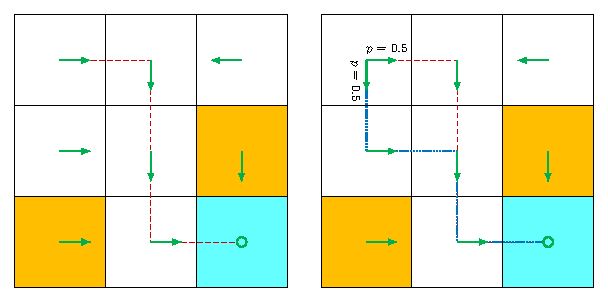
\includegraphics[width=291.9pt]{fig3_3}\par\smallskip
  \begin{minipage}{0.94\textwidth}\footnotesize
  \textbf{Figure 3.3.} Examples for demonstrating that optimal policies may not be unique. The two policies are different but are both optimal.\par\smallskip
  \textcolor{rulegray}{\scriptsize Reproduced from S.~Zhao, \emph{Mathematical Foundations of Reinforcement Learning} (Springer, 2025).}
  \end{minipage}
\end{figure}


\subsection{What actually determines the optimal policy}

\bk{\S3.5, pp.~49--53; Figure 3.4, p.~50}
\ \vid{L3 P4}{https://www.youtube.com/watch?v=a--bck2ow9s}

Only three things appear in the BOE, so only three things can matter:
(i) the rewards $r$; (ii) the discount rate $\gamma$; (iii) the model
$p(s'\mid s,a),p(r\mid s,a)$. The model is given, so the book varies the other two
on a $5\times5$ grid \bkin{\S3.5, pp.~49--53}.

\begin{worked}{the discount rate changes the personality of the agent \bkin{Figure 3.4, p.~50}}
Baseline: $r_{\text{boundary}}=r_{\text{forbidden}}=-1$, $r_{\text{target}}=1$,
$r_{\text{other}}=0$, $\gamma=0.9$.

\textbf{(a) $\gamma=0.9$.} Optimal values, row by row:
\[
\begin{array}{ccccc}
5.8&5.6&6.2&6.5&5.8\\
6.5&7.2&8.0&7.2&6.5\\
7.2&8.0&10.0&8.0&7.2\\
8.0&10.0&10.0&10.0&8.0\\
7.2&9.0&10.0&9.0&8.1
\end{array}
\]
The striking behaviour: starting from row 4, column 1, the optimal policy is
willing to \emph{cut straight through forbidden cells}, eating $-1$ penalties,
because the shortcut to the target is worth more in discounted terms than the long
safe detour. The agent is far-sighted.

\textbf{(b) $\gamma=0.5$.} Same rewards, different attitude: the agent no longer
dares take the risk and travels the long way round, avoiding every forbidden cell.
Values collapse toward zero except near the target ($2.0$ at the target, $0.1$ or
$0.0$ far away).

\textbf{(c) $\gamma=0$.} The agent maximises only the immediate reward. It becomes
completely myopic and \emph{never reaches the target at all} from most cells. All
values are $0$ except $1.0$ in the cells adjacent to/at the target.
\end{worked}

\begin{remark}[The spatial pattern]
Across all these grids, states closer to the target have larger values. The reason
is purely the discount rate: a distant state needs a longer trajectory before it
collects the $+1$, and $\gamma^k$ shrinks it \bkin{\S3.5, p.~51}.
\end{remark}

\begin{figure}[htbp]
  \centering
  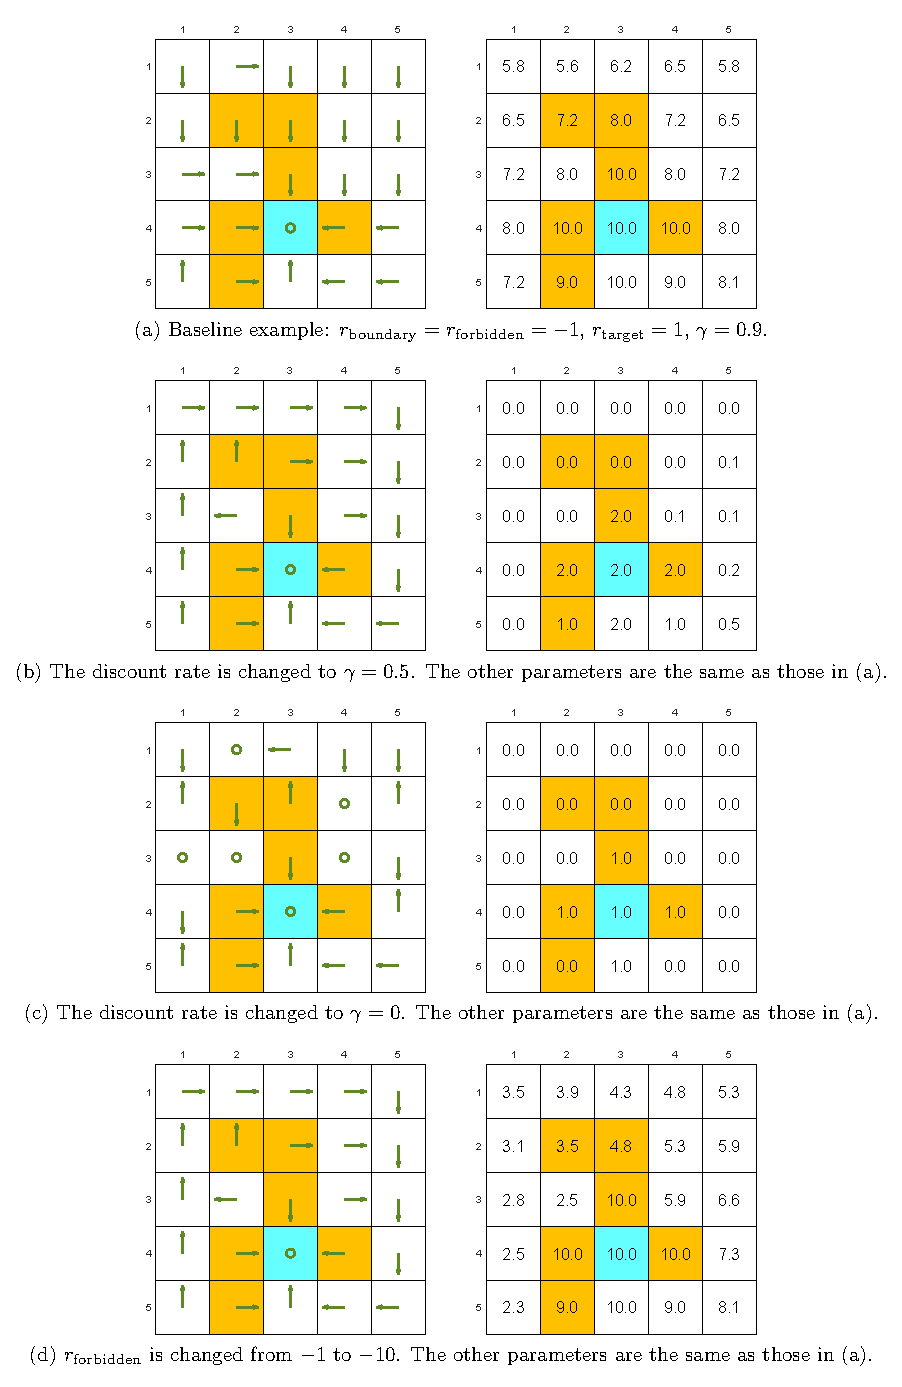
\includegraphics[width=262.1pt]{fig3_4}\par\smallskip
  \begin{minipage}{0.94\textwidth}\footnotesize
  \textbf{Figure 3.4.} The optimal policies and optimal state values given different parameter values.\par\smallskip
  \textcolor{rulegray}{\scriptsize Reproduced from S.~Zhao, \emph{Mathematical Foundations of Reinforcement Learning} (Springer, 2025).}
  \end{minipage}
\end{figure}


\begin{worked}{changing a reward can change the optimal policy \bkin{Figure 3.4(d), p.~50}}
Keep $\gamma=0.9$ but change $r_{\text{forbidden}}$ from $-1$ to $-10$. Now the
optimal policy \emph{never} enters a forbidden cell. The value grid becomes
\[
\begin{array}{ccccc}
3.5&3.9&4.3&4.8&5.3\\
3.1&3.5&4.8&5.3&5.9\\
2.8&2.5&10.0&5.9&6.6\\
2.5&10.0&10.0&10.0&7.3\\
2.3&9.0&10.0&9.0&8.1
\end{array}
\]
So reward design is a real lever. But --- and this is the subtle part --- not every
change to the rewards is a real change.
\end{worked}

\begin{theorem}[Optimal policy invariance --- Theorem 3.6, p.~51; equation (3.8)]
If every reward $r$ is replaced by $\alpha r+\beta$ with $\alpha>0$, then the
optimal state value becomes
\[
  v' = \alpha v^* + \frac{\beta}{1-\gamma}\mathbf{1},
\]
and the greedy policy derived from $v'$ is the same as the one derived from $v^*$.
\end{theorem}

\begin{proof}[Proof (Box 3.5, pp.~51--52)]
Under $r\mapsto\alpha r+\beta$ we get $r_\pi\mapsto\alpha r_\pi+\beta\mathbf 1$, so
the new BOE is $v'=\max_\pi(\alpha r_\pi+\beta\mathbf1+\gamma P_\pi v')$. Guess
$v'=\alpha v^*+c\mathbf1$ and substitute, using $P_\pi\mathbf1=\mathbf1$:
\[
  \alpha v^*+c\mathbf1=\max_\pi(\alpha r_\pi+\alpha\gamma P_\pi v^*)+\beta\mathbf1+c\gamma\mathbf1
  \;\Longrightarrow\; \beta+c\gamma-c=0 \;\Longrightarrow\; c=\frac{\beta}{1-\gamma}.
\]
Since the BOE has a unique solution, this guess \emph{is} the solution. An affine
transformation preserves the ordering of the $q$-values, so the argmax is unchanged.
\end{proof}

\begin{warning}[Do you need a step penalty to prevent dithering?]
\bkin{\S3.5, pp.~52--53; Figure 3.5, p.~52}
A near-universal beginner instinct: since $r_{\text{other}}=0$, wandering costs
nothing, so surely we must add $-1$ per step to make the agent hurry? \textbf{No,
twice over.}

\emph{First}, adding a constant to every reward is an affine transformation, so by
Theorem 3.6 it changes nothing about the optimal policy.

\emph{Second}, the discount rate already does the job. The book's Figure 3.5 (p.~52)
compares two policies in a $2\times2$ grid with the target at the bottom right.
The direct policy $s_2\to s_4$ earns
\[
  1+\gamma+\gamma^2+\cdots=\frac{1}{1-\gamma}=10,
\]
whereas the dithering policy $s_2\to s_1\to s_3\to s_4$ earns
\[
  0+\gamma\cdot0+\gamma^2(1+\gamma+\cdots)=\frac{\gamma^2}{1-\gamma}=8.1 .
\]
Ten beats $8.1$: \emph{the detour is punished automatically, because the reward it
eventually collects arrives two periods later and is discounted twice.} An
economist will recognise this instantly --- it is just the time value of money.
\end{warning}

\begin{figure}[htbp]
  \centering
  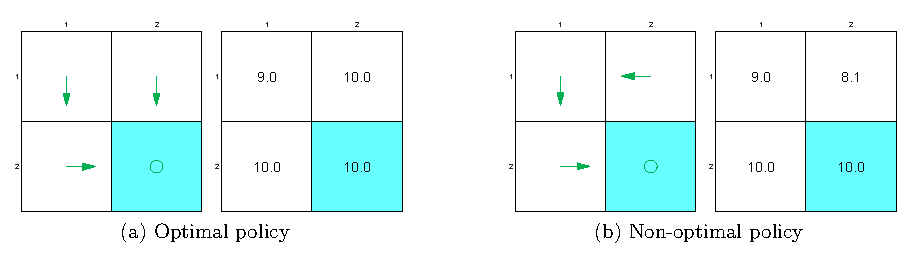
\includegraphics[width=437.1pt]{fig3_5}\par\smallskip
  \begin{minipage}{0.94\textwidth}\footnotesize
  \textbf{Figure 3.5.} Examples illustrating that optimal policies do not take meaningless detours due to the discount rate.\par\smallskip
  \textcolor{rulegray}{\scriptsize Reproduced from S.~Zhao, \emph{Mathematical Foundations of Reinforcement Learning} (Springer, 2025).}
  \end{minipage}
\end{figure}


\subsection{Chapter 3 self-check}

\begin{enumerate}
  \item Why does the BOE have two unknowns, and what is the two-step trick that
        resolves this? \emph{(Example 3.1, p.~39.)}
  \item State the three conclusions of the contraction mapping theorem and match
        each to a question about optimal policies (existence / uniqueness /
        computation).
  \item Prove in one line that if $q^*(s,a_1)=q^*(s,a_2)>q^*(s,a)$ for all other
        $a$, then the policy putting probability $0.3$ on $a_1$ and $0.7$ on $a_2$
        is also optimal.
  \item Your agent takes a long safe route instead of a fast risky one, and you
        want it to be bolder. Name two parameters you could change and say what
        each would do. \emph{(Raise $\gamma$; or reduce $|r_{\text{forbidden}}|$;
        \bkin{\S3.5, pp.~49--51}.)}
  \item True or false: adding $+100$ to every reward makes the agent reach the
        target faster. \emph{(False --- Theorem 3.6.)}
\end{enumerate}

\newpage
% ============================================================
\section{Value Iteration and Policy Iteration}
% ============================================================

\begin{roadmap}{Chapter 4 of the textbook}
\textbf{Textbook:} Chapter 4, pp.~57--76. Sections: \S4.1 value iteration (p.~58;
elementwise form p.~58, examples p.~59), \S4.2 policy iteration (p.~62; analysis
p.~62, elementwise form p.~65, examples p.~67), \S4.3 truncated policy iteration
(p.~70; comparison p.~70, algorithm p.~72), \S4.4 summary (p.~74), \S4.5 Q\&A
(p.~74). Algorithms 4.1 (p.~60), 4.2 (p.~66), 4.3 (p.~72).\\[0.3em]
\textbf{Videos:}
\vid{L4 P1 --- Value iteration}{https://www.youtube.com/watch?v=wMAVmLDIvQU};
\vid{L4 P2 --- Policy iteration}{https://www.youtube.com/watch?v=Pka6Om0nYQ8};
\vid{L4 P3 --- Truncated policy iteration}{https://www.youtube.com/watch?v=tUjPFPD3Vc8}.\\[0.3em]
\textbf{Status of these algorithms:} they are \textbf{dynamic programming}, not
really reinforcement learning, because they require the model
$\{p(r\mid s,a),p(s'\mid s,a)\}$ \bkin{\S4.1, p.~58}. They matter because every
model-free algorithm in Chapters 5--10 is obtained by replacing one step of one of
them with a sample estimate.
\end{roadmap}

\begin{figure}[htbp]
  \centering
  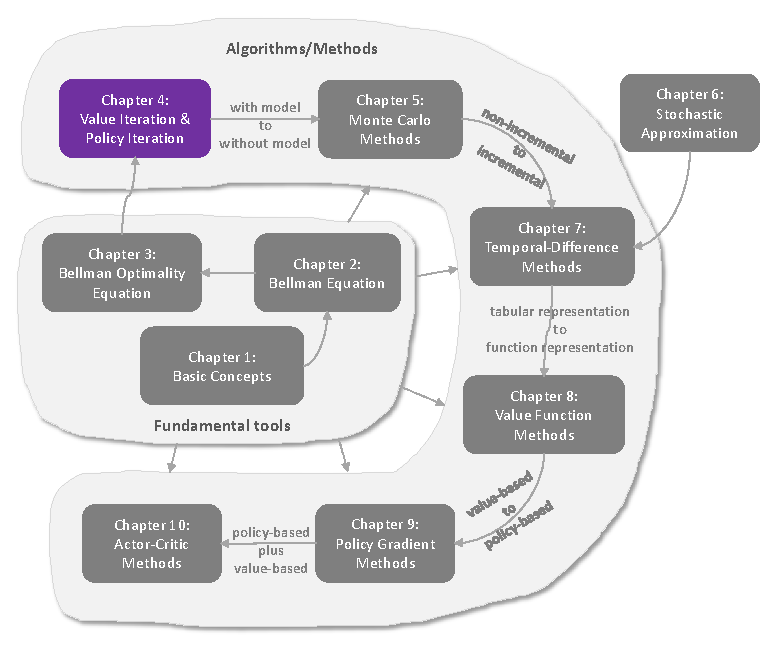
\includegraphics[width=371.3pt]{fig4_1}\par\smallskip
  \begin{minipage}{0.94\textwidth}\footnotesize
  \textbf{Figure 4.1.} Where we are in this book.\par\smallskip
  \textcolor{rulegray}{\scriptsize Reproduced from S.~Zhao, \emph{Mathematical Foundations of Reinforcement Learning} (Springer, 2025).}
  \end{minipage}
\end{figure}


\subsection{Value iteration}

\bk{\S4.1, pp.~58--59; Algorithm 4.1, p.~60}

Value iteration \emph{is} the contraction iteration of Theorem 3.3:
\[
  v_{k+1}=\max_{\pi\in\Pi}\bigl(r_\pi+\gamma P_\pi v_k\bigr),\qquad k=0,1,2,\dots
\]
Split each iteration into two named steps \bkin{\S4.1, p.~58}:

\begin{enumerate}
  \item \textbf{Policy update (PU):} $\pi_{k+1}=\argmax_\pi(r_\pi+\gamma P_\pi v_k)$.
  \item \textbf{Value update (VU):} $v_{k+1}=r_{\pi_{k+1}}+\gamma P_{\pi_{k+1}}v_k$
        \bkin{equation (4.1), p.~58}.
\end{enumerate}

\subsubsection{Elementwise form --- what you actually code}

\bk{\S4.1.1, pp.~58--59}

For each state $s$, first compute the $q$-values from the current $v_k$:
\[
  q_k(s,a)=\sum_{r}p(r\mid s,a)\,r+\gamma\sum_{s'}p(s'\mid s,a)\,v_k(s').
\]
Then
\[
  a_k^*(s)=\argmax_a q_k(s,a),\qquad
  \pi_{k+1}(a\mid s)=\begin{cases}1,&a=a_k^*(s)\\0,&\text{otherwise,}\end{cases}
  \qquad
  v_{k+1}(s)=\max_a q_k(s,a).
\]
The book summarises the flow as \bkin{\S4.1.1, p.~59}
\[
  v_k(s)\ \to\ q_k(s,a)\ \to\ \text{greedy }\pi_{k+1}(s)\ \to\ v_{k+1}(s)=\max_a q_k(s,a).
\]

\begin{algobox}{Value iteration (Algorithm 4.1, p.~60)}
\textbf{Input:} the model $p(r\mid s,a)$, $p(s'\mid s,a)$ for all $(s,a)$; an initial
guess $v_0$.\\
\textbf{While} $\norm{v_k-v_{k-1}}$ exceeds a small threshold, \textbf{do}
\begin{itemize}\itemsep0pt
  \item For every $s\in\Sspace$:
  \begin{itemize}\itemsep0pt
    \item For every $a\in\Aspace(s)$:\quad
          $q_k(s,a)=\sum_r p(r\mid s,a)r+\gamma\sum_{s'}p(s'\mid s,a)v_k(s')$
    \item $a_k^*(s)=\argmax_a q_k(s,a)$
    \item Policy update: $\pi_{k+1}(a\mid s)=1$ if $a=a_k^*(s)$, else $0$
    \item Value update: $v_{k+1}(s)=\max_a q_k(s,a)$
  \end{itemize}
\end{itemize}
\end{algobox}

\begin{warning}
$v_k$ is \textbf{not a state value}. It does not satisfy the Bellman equation of
$\pi_k$ or of $\pi_{k+1}$ or of any policy. It is a numerical iterate that happens
to converge to $v^*$. Consequently $q_k$ is not an action value either
\bkin{\S4.1.1, p.~59 and \S4.5 Q\&A, p.~74}. Contrast this with policy iteration
below, where the intermediate values \emph{are} genuine state values.
\end{warning}

\subsubsection{A complete numerical run}

\bk{\S4.1.2, pp.~59--62; Figure 4.2, p.~60; Tables 4.1--4.3, pp.~60--61}

The book's example is a $2\times2$ grid: $s_1,s_2$ on top, $s_3,s_4$ beneath;
$s_2$ is forbidden, $s_4$ is the target;
$r_{\text{boundary}}=r_{\text{forbidden}}=-1$, $r_{\text{target}}=1$, $\gamma=0.9$.

First write out the $q$-value expressions once (the book's Table 4.1, p.~60):

\begin{center}
\small
\begin{tabular}{@{}lccccc@{}}
\toprule
$q(s,a)$ & $a_1$ (up) & $a_2$ (right) & $a_3$ (down) & $a_4$ (left) & $a_5$ (stay)\\
\midrule
$s_1$ & $-1+\gamma v(s_1)$ & $-1+\gamma v(s_2)$ & $0+\gamma v(s_3)$ & $-1+\gamma v(s_1)$ & $0+\gamma v(s_1)$\\
$s_2$ & $-1+\gamma v(s_2)$ & $-1+\gamma v(s_2)$ & $1+\gamma v(s_4)$ & $0+\gamma v(s_1)$ & $-1+\gamma v(s_2)$\\
$s_3$ & $0+\gamma v(s_1)$ & $1+\gamma v(s_4)$ & $-1+\gamma v(s_3)$ & $-1+\gamma v(s_3)$ & $0+\gamma v(s_3)$\\
$s_4$ & $-1+\gamma v(s_2)$ & $-1+\gamma v(s_4)$ & $-1+\gamma v(s_4)$ & $0+\gamma v(s_3)$ & $1+\gamma v(s_4)$\\
\bottomrule
\end{tabular}
\end{center}

\begin{worked}{value iteration, iteration by iteration \bkin{\S4.1.2, pp.~60--61}}
\textbf{$k=0$: start from $v_0=(0,0,0,0)$.}

Substituting into the table gives the book's Table 4.2 (p.~61):
\begin{center}
\small
\begin{tabular}{@{}lccccc@{}}
\toprule
$q_0$ & $a_1$ & $a_2$ & $a_3$ & $a_4$ & $a_5$\\
\midrule
$s_1$ & $-1$ & $-1$ & $0$ & $-1$ & $0$\\
$s_2$ & $-1$ & $-1$ & $1$ & $0$ & $-1$\\
$s_3$ & $0$ & $1$ & $-1$ & $-1$ & $0$\\
$s_4$ & $-1$ & $-1$ & $-1$ & $0$ & $1$\\
\bottomrule
\end{tabular}
\end{center}
Greedy policy: $\pi_1(a_5\mid s_1)=1$, $\pi_1(a_3\mid s_2)=1$,
$\pi_1(a_2\mid s_3)=1$, $\pi_1(a_5\mid s_4)=1$. (At $s_1$ the actions $a_3$ and
$a_5$ tie at $0$; either may be taken without affecting convergence
\bkin{\S4.1.1, p.~59}.) This policy is visibly not optimal --- it stays put at
$s_1$. Value update: $v_1=(0,1,1,1)$.

\textbf{$k=1$: substitute $v_1=(0,1,1,1)$, $\gamma=0.9$} (the book's Table 4.3, p.~61):
\begin{center}
\small
\begin{tabular}{@{}lccccc@{}}
\toprule
$q_1$ & $a_1$ & $a_2$ & $a_3$ & $a_4$ & $a_5$\\
\midrule
$s_1$ & $-1+0=-1$ & $-1+0.9=-0.1$ & $0+0.9=\mathbf{0.9}$ & $-1$ & $0$\\
$s_2$ & $-0.1$ & $-0.1$ & $1+0.9=\mathbf{1.9}$ & $0$ & $-0.1$\\
$s_3$ & $0$ & $1+0.9=\mathbf{1.9}$ & $-0.1$ & $-0.1$ & $0.9$\\
$s_4$ & $-0.1$ & $-0.1$ & $-0.1$ & $0.9$ & $1+0.9=\mathbf{1.9}$\\
\bottomrule
\end{tabular}
\end{center}
Greedy policy: $\pi_2(a_3\mid s_1)=1$, $\pi_2(a_3\mid s_2)=1$,
$\pi_2(a_2\mid s_3)=1$, $\pi_2(a_5\mid s_4)=1$. Value update:
$v_2=(0.9,\,1.9,\,1.9,\,1.9)$.

\textbf{Result.} $\pi_2$ is already optimal --- two iterations sufficed for this
tiny example \bkin{\S4.1.2, p.~62}. The \emph{values} keep improving for many more
iterations (they converge to $(9,10,10,10)$ in the limit), but the \emph{policy}
has already stopped changing. This gap between "the policy has converged" and "the
values have converged" recurs throughout the book.
\end{worked}

\begin{figure}[htbp]
  \centering
  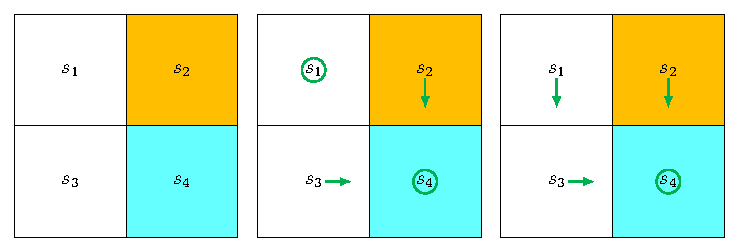
\includegraphics[width=354.6pt]{fig4_2}\par\smallskip
  \begin{minipage}{0.94\textwidth}\footnotesize
  \textbf{Figure 4.2.} An example for demonstrating the implementation of the value iteration algorithm.\par\smallskip
  \textcolor{rulegray}{\scriptsize Reproduced from S.~Zhao, \emph{Mathematical Foundations of Reinforcement Learning} (Springer, 2025).}
  \end{minipage}
\end{figure}


\subsection{Policy iteration}

\bk{\S4.2, pp.~62--69; Algorithm 4.2, p.~66}

Policy iteration does not attack the BOE directly. It alternates:

\begin{itemize}
  \item \textbf{Policy evaluation (PE):} given $\pi_k$, solve the \emph{linear}
        Bellman equation $v_{\pi_k}=r_{\pi_k}+\gamma P_{\pi_k}v_{\pi_k}$
        \bkin{equation (4.3), p.~62}.
  \item \textbf{Policy improvement (PI):} given $v_{\pi_k}$, set
        $\pi_{k+1}=\argmax_\pi(r_\pi+\gamma P_\pi v_{\pi_k})$.
\end{itemize}

Three questions must be answered \bkin{\S4.2.1, p.~62}: how do we solve the
evaluation step, why is $\pi_{k+1}$ better than $\pi_k$, and why does the whole
thing converge?

\subsubsection{Answer 1: how to evaluate}

Chapter 2 gave two ways. The closed form $v_{\pi_k}=(I-\gamma P_{\pi_k})^{-1}r_{\pi_k}$
is impractical; instead use the inner iteration \bkin{equation (4.4), p.~63}
\[
  v_{\pi_k}^{(j+1)}=r_{\pi_k}+\gamma P_{\pi_k}v_{\pi_k}^{(j)},\qquad j=0,1,2,\dots
\]
which converges as $j\to\infty$ from any $v^{(0)}_{\pi_k}$.

\begin{remark}
So policy iteration is an iterative algorithm with a \emph{second} iterative
algorithm nested inside it. In theory the inner loop needs infinitely many steps;
in practice you stop when $\norm{v^{(j+1)}-v^{(j)}}$ is small or when $j$ hits a
cap. Does stopping early break things? No --- and understanding why is exactly the
point of truncated policy iteration in \S4.3 \bkin{\S4.2.1, p.~63}.
\end{remark}

\subsubsection{Answer 2: improvement really improves}

\begin{lemma}[Policy improvement --- Lemma 4.1, p.~63]
If $\pi_{k+1}=\argmax_\pi(r_\pi+\gamma P_\pi v_{\pi_k})$, then
$v_{\pi_{k+1}}\ \ge\ v_{\pi_k}$ elementwise.
\end{lemma}

\begin{proof}[Proof (Box 4.1, pp.~63--64)]
Both are state values, so $v_{\pi_{k+1}}=r_{\pi_{k+1}}+\gamma P_{\pi_{k+1}}v_{\pi_{k+1}}$
and $v_{\pi_k}=r_{\pi_k}+\gamma P_{\pi_k}v_{\pi_k}$. By construction of $\pi_{k+1}$,
$r_{\pi_{k+1}}+\gamma P_{\pi_{k+1}}v_{\pi_k}\ \ge\ r_{\pi_k}+\gamma P_{\pi_k}v_{\pi_k}$.
Therefore
\[
  v_{\pi_k}-v_{\pi_{k+1}}
  \le \bigl(r_{\pi_{k+1}}+\gamma P_{\pi_{k+1}}v_{\pi_k}\bigr)
     -\bigl(r_{\pi_{k+1}}+\gamma P_{\pi_{k+1}}v_{\pi_{k+1}}\bigr)
  = \gamma P_{\pi_{k+1}}\bigl(v_{\pi_k}-v_{\pi_{k+1}}\bigr).
\]
Iterating, $v_{\pi_k}-v_{\pi_{k+1}}\le\gamma^nP^n_{\pi_{k+1}}(v_{\pi_k}-v_{\pi_{k+1}})\to0$.
\end{proof}

\subsubsection{Answer 3: convergence}

\begin{theorem}[Convergence of policy iteration --- Theorem 4.1, p.~64]
The state-value sequence $\{v_{\pi_k}\}_{k=0}^\infty$ converges to $v^*$, and hence
$\{\pi_k\}$ converges to an optimal policy.
\end{theorem}

\begin{proof}[Proof idea (Box 4.2, p.~65)]
By Lemma 4.1 the sequence is nondecreasing, and it is bounded above by $v^*$:
\[
  v_{\pi_0}\le v_{\pi_1}\le v_{\pi_2}\le\cdots\le v^* .
\]
By the monotone convergence theorem it converges to some $v_\infty$. To show
$v_\infty=v^*$, run value iteration $v_{k+1}=f(v_k)$ alongside, started at
$v_0\le v_{\pi_0}$, and prove by induction that $v_k\le v_{\pi_k}\le v^*$ for all
$k$. Since $v_k\to v^*$, the sandwich forces $v_{\pi_k}\to v^*$.
\end{proof}

\begin{intuition}
The proof does more than establish convergence --- it shows \textbf{policy
iteration converges at least as fast as value iteration}, iteration for iteration,
because it squeezes in extra evaluation sweeps. It is not free: each of those
sweeps costs computation \bkin{\S4.2.1, p.~64}.
\end{intuition}

\begin{algobox}{Policy iteration (Algorithm 4.2, p.~66)}
\textbf{Input:} the model; an initial policy $\pi_0$.\\
\textbf{While} $v_{\pi_k}$ has not converged, \textbf{do}
\begin{itemize}\itemsep0pt
  \item \textbf{Policy evaluation.} Initialise $v^{(0)}_{\pi_k}$ arbitrarily.
        While not converged, for every $s$:
        \[
          v_{\pi_k}^{(j+1)}(s)=\sum_a\pi_k(a\mid s)
            \Bigl[\sum_r p(r\mid s,a)r+\gamma\sum_{s'}p(s'\mid s,a)v^{(j)}_{\pi_k}(s')\Bigr]
        \]
  \item \textbf{Policy improvement.} For every $s$ and every $a$:
        $q_{\pi_k}(s,a)=\sum_r p(r\mid s,a)r+\gamma\sum_{s'}p(s'\mid s,a)v_{\pi_k}(s')$;
        then $a_k^*(s)=\argmax_a q_{\pi_k}(s,a)$ and
        $\pi_{k+1}(a\mid s)=1$ if $a=a_k^*(s)$, else $0$.
\end{itemize}
\end{algobox}

\subsubsection{A two-state example done by hand}

\bk{\S4.2.3, pp.~67--68; Figure 4.3, p.~67; Tables 4.4--4.5, p.~68}

Two states $s_1,s_2$; three actions $\Aspace=\{a_\ell,a_0,a_r\}$ (left, stay,
right); $s_2$ is the target; $r_{\text{boundary}}=-1$, $r_{\text{target}}=1$,
$\gamma=0.9$. The initial policy $\pi_0$ moves \emph{away} from the target at $s_1$
and drifts at $s_2$.

\begin{worked}{one full iteration of policy iteration \bkin{\S4.2.3, pp.~67--68}}
\textbf{Policy evaluation.} The Bellman equations of $\pi_0$ are
\[
  v_{\pi_0}(s_1)=-1+\gamma v_{\pi_0}(s_1),\qquad
  v_{\pi_0}(s_2)=0+\gamma v_{\pi_0}(s_1).
\]
By hand: $v_{\pi_0}(s_1)=-1/(1-0.9)=-10$ and $v_{\pi_0}(s_2)=0.9(-10)=-9$.

If instead you run the iterative solver from $v^{(0)}=(0,0)$ you get
\[
\begin{aligned}
  v^{(1)}&=(-1,\;0), &
  v^{(2)}&=(-1.9,\;-0.9), &
  v^{(3)}&=(-2.71,\;-1.71),\ \dots
\end{aligned}
\]
crawling toward $(-10,-9)$ --- exactly the geometric convergence promised in
\S2.7.2.

\textbf{Policy improvement.} The $q$-table (the book's Table 4.4, p.~68) is
\begin{center}
\small
\begin{tabular}{@{}lccc@{}}
\toprule
$q_{\pi_k}(s,a)$ & $a_\ell$ & $a_0$ & $a_r$\\
\midrule
$s_1$ & $-1+\gamma v_{\pi_k}(s_1)$ & $0+\gamma v_{\pi_k}(s_1)$ & $1+\gamma v_{\pi_k}(s_2)$\\
$s_2$ & $0+\gamma v_{\pi_k}(s_1)$ & $1+\gamma v_{\pi_k}(s_2)$ & $-1+\gamma v_{\pi_k}(s_2)$\\
\bottomrule
\end{tabular}
\end{center}
Substituting $v_{\pi_0}=(-10,-9)$ gives Table 4.5, p.~68:
\begin{center}
\small
\begin{tabular}{@{}lccc@{}}
\toprule
$q_{\pi_0}(s,a)$ & $a_\ell$ & $a_0$ & $a_r$\\
\midrule
$s_1$ & $-10$ & $-9$ & $\mathbf{-7.1}$\\
$s_2$ & $-9$ & $\mathbf{-7.1}$ & $-9.1$\\
\bottomrule
\end{tabular}
\end{center}
Greedy: $\pi_1(a_r\mid s_1)=1$ and $\pi_1(a_0\mid s_2)=1$. \textbf{That is the
optimal policy}, found in a single iteration.

Note that all the $q$-values are negative and yet the improvement step works
perfectly. Only the \emph{ordering} matters, never the sign --- another face of
Theorem 3.6.
\end{worked}

\begin{figure}[htbp]
  \centering
  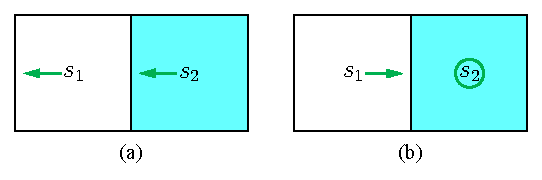
\includegraphics[width=260.0pt]{fig4_3}\par\smallskip
  \begin{minipage}{0.94\textwidth}\footnotesize
  \textbf{Figure 4.3.} An example for illustrating the implementation of the policy iteration algorithm.\par\smallskip
  \textcolor{rulegray}{\scriptsize Reproduced from S.~Zhao, \emph{Mathematical Foundations of Reinforcement Learning} (Springer, 2025).}
  \end{minipage}
\end{figure}


\subsubsection{A $5\times5$ example: how learning spreads}

\bk{\S4.2.3, pp.~68--69; Figure 4.4, p.~69}

The book runs policy iteration on a $5\times5$ grid with
$r_{\text{boundary}}=-1$, $r_{\text{forbidden}}=-10$, $r_{\text{target}}=1$,
$\gamma=0.9$, starting from a random policy $\pi_0$. It converges to the optimal
policy $\pi_{10}$ after ten iterations. Two patterns are worth memorising
\bkin{\S4.2.3, pp.~68--69}:

\begin{itemize}
  \item \textbf{Optimality propagates outward from the target.} States adjacent to
        the target settle on their optimal actions first; distant states can only
        find good routes once the nearby states have found theirs. At $\pi_1$ only
        the cells around the target have nonzero values ($10.0$, $9.0$); by
        $\pi_5$ the right-hand column has filled in ($4.3,\,4.8,\,5.3,\dots$); only
        at $\pi_{10}$ does the far-left column acquire its values
        ($3.5,\,3.1,\,2.8,\,2.5,\,2.3$).
  \item \textbf{Values decline with distance from the target}, for the discounting
        reason already met in \S3.5.
\end{itemize}

\begin{figure}[htbp]
  \centering
  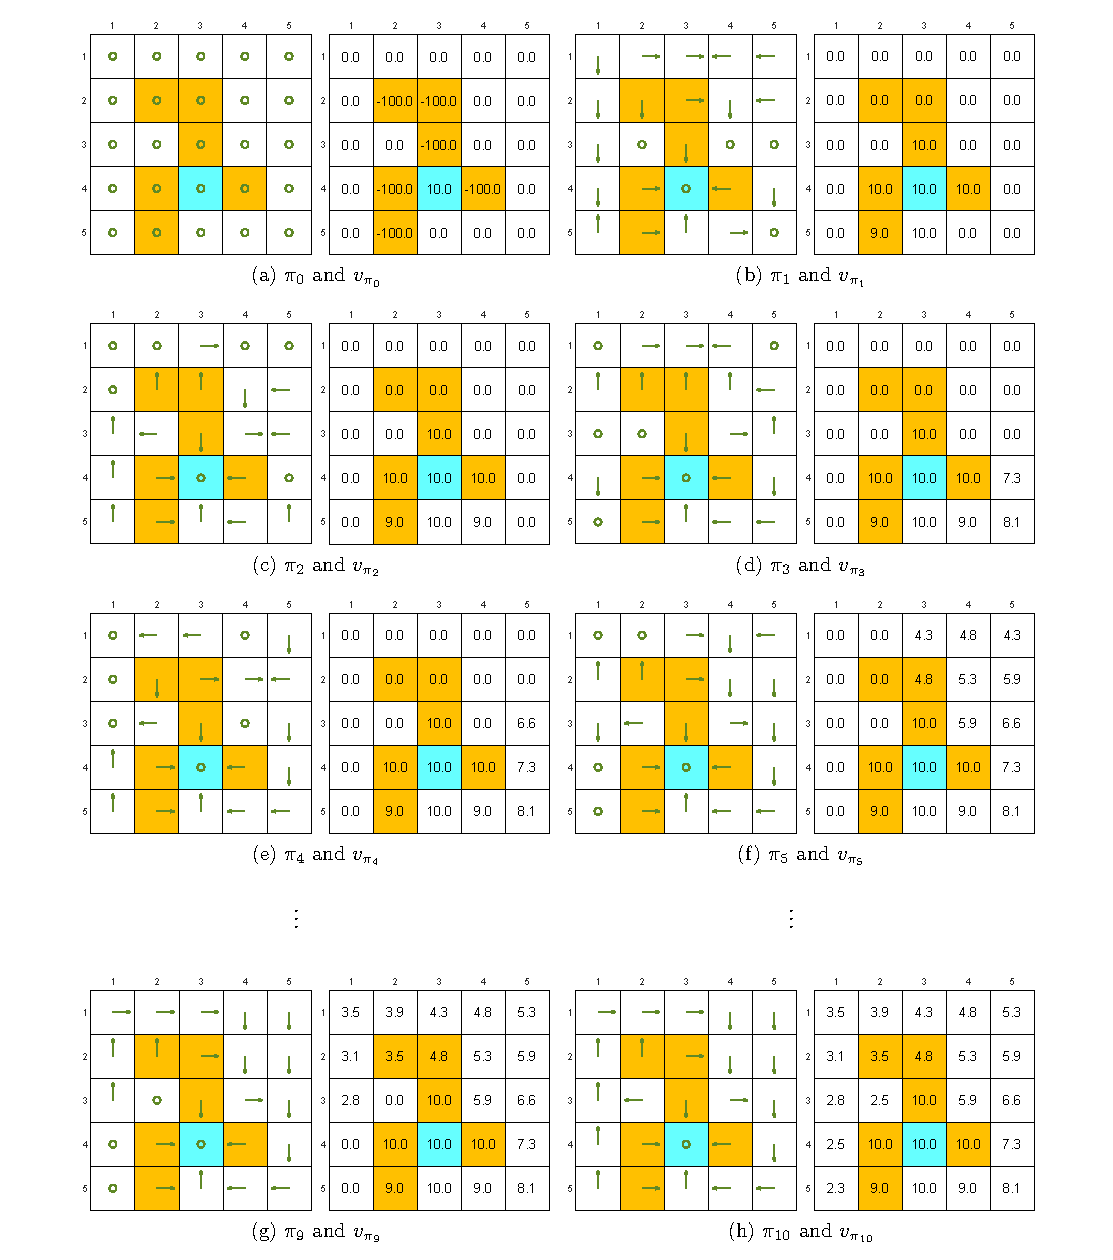
\includegraphics[width=355.8pt]{fig4_4}\par\smallskip
  \begin{minipage}{0.94\textwidth}\footnotesize
  \textbf{Figure 4.4.} The evolution processes of the policies generated by the policy iteration algorithm.\par\smallskip
  \textcolor{rulegray}{\scriptsize Reproduced from S.~Zhao, \emph{Mathematical Foundations of Reinforcement Learning} (Springer, 2025).}
  \end{minipage}
\end{figure}


\subsection{Truncated policy iteration}

\bk{\S4.3, pp.~70--74; Table 4.6, p.~71; Algorithm 4.3, p.~72}

\subsubsection{The two algorithms are the same algorithm}

\bk{\S4.3.1, pp.~70--72}

Lay them side by side \bkin{\S4.3.1, p.~70}:
\[
\begin{aligned}
  \text{Policy iteration:}&\quad
  \pi_0\xrightarrow{\text{PE}}v_{\pi_0}\xrightarrow{\text{PI}}\pi_1
  \xrightarrow{\text{PE}}v_{\pi_1}\xrightarrow{\text{PI}}\pi_2\to\cdots\\
  \text{Value iteration:}&\quad
  v_0\xrightarrow{\text{PU}}\pi_1'\xrightarrow{\text{VU}}v_1
  \xrightarrow{\text{PU}}\pi_2'\xrightarrow{\text{VU}}v_2\to\cdots
\end{aligned}
\]
Start both from the same place, $v_0=v_{\pi_0}$. Then steps 1--3 produce identical
results. They diverge at step 4 \bkin{Table 4.6, p.~71}: value iteration computes
the single line $v_1=r_{\pi_1}+\gamma P_{\pi_1}v_0$, whereas policy iteration
solves $v_{\pi_1}=r_{\pi_1}+\gamma P_{\pi_1}v_{\pi_1}$ --- an infinite loop. Write
that loop out with $v^{(0)}_{\pi_1}=v_0$:
\[
\begin{aligned}
  v^{(0)}_{\pi_1}&=v_0\\
  v^{(1)}_{\pi_1}&=r_{\pi_1}+\gamma P_{\pi_1}v^{(0)}_{\pi_1}
    &&\longleftarrow\ \textbf{value iteration stops here}\\
  v^{(2)}_{\pi_1}&=r_{\pi_1}+\gamma P_{\pi_1}v^{(1)}_{\pi_1}\\
  &\ \ \vdots\\
  v^{(j_{\text{truncate}})}_{\pi_1}&=\cdots
    &&\longleftarrow\ \textbf{truncated policy iteration stops here}\\
  &\ \ \vdots\\
  v^{(\infty)}_{\pi_1}&=r_{\pi_1}+\gamma P_{\pi_1}v^{(\infty)}_{\pi_1}
    &&\longleftarrow\ \textbf{policy iteration stops here}
\end{aligned}
\]

\begin{remark}
So there is one algorithm with one dial, $j_{\text{truncate}}$:
\[
  j_{\text{truncate}}=1\ \Rightarrow\ \text{value iteration};\qquad
  j_{\text{truncate}}=\infty\ \Rightarrow\ \text{policy iteration};\qquad
  1<j_{\text{truncate}}<\infty\ \Rightarrow\ \text{truncated policy iteration}.
\]
This is one of the tidiest unifications in the book \bkin{\S4.3.1, pp.~71--72}.
\end{remark}

\begin{algobox}{Truncated policy iteration (Algorithm 4.3, p.~72)}
\textbf{Input:} the model; an initial policy $\pi_0$; a cap $j_{\text{truncate}}$.\\
\textbf{While} $v_k$ has not converged, \textbf{do}
\begin{itemize}\itemsep0pt
  \item \textbf{Policy evaluation (truncated).} Set $v_k^{(0)}=v_{k-1}$.
        For $j=0,\dots,j_{\text{truncate}}-1$ and every $s$:
        \[
          v_k^{(j+1)}(s)=\sum_a\pi_k(a\mid s)
            \Bigl[\sum_r p(r\mid s,a)r+\gamma\sum_{s'}p(s'\mid s,a)v_k^{(j)}(s')\Bigr].
        \]
        Set $v_k=v_k^{(j_{\text{truncate}})}$.
  \item \textbf{Policy improvement.} For every $s$, compute
        $q_k(s,a)=\sum_r p(r\mid s,a)r+\gamma\sum_{s'}p(s'\mid s,a)v_k(s')$ and set
        $\pi_{k+1}(a\mid s)=1$ if $a=\argmax_{a'}q_k(s,a')$, else $0$.
\end{itemize}
\end{algobox}

\subsubsection{Does truncation break convergence?}

\bk{\S4.3.2, pp.~72--74; Proposition 4.1, p.~72; Figure 4.5, p.~73}

No. The intermediate $v_k$ are only \emph{approximations} of $v_{\pi_k}$, but the
algorithm still finds optimal policies, and it sits neatly between the two extremes
--- faster than value iteration (more evaluation per improvement), slower than
full policy iteration (fewer evaluations) \bkin{\S4.3.2, p.~72; Figure 4.5, p.~73}.

\begin{proposition}[Value improvement --- Proposition 4.1, p.~72]
In the inner loop $v^{(j+1)}_{\pi_k}=r_{\pi_k}+\gamma P_{\pi_k}v^{(j)}_{\pi_k}$, if
the initial guess is $v^{(0)}_{\pi_k}=v_{\pi_{k-1}}$, then
$v^{(j+1)}_{\pi_k}\ge v^{(j)}_{\pi_k}$ for all $j$: the inner iterates climb
monotonically.
\end{proposition}

\begin{proof}[Proof (Box 4.3, p.~73)]
Subtracting consecutive inner iterations gives
$v^{(j+1)}_{\pi_k}-v^{(j)}_{\pi_k}=\gamma^jP^j_{\pi_k}\bigl(v^{(1)}_{\pi_k}-v^{(0)}_{\pi_k}\bigr)$,
the book's equation (4.5). And with $v^{(0)}_{\pi_k}=v_{\pi_{k-1}}$,
\[
  v^{(1)}_{\pi_k}=r_{\pi_k}+\gamma P_{\pi_k}v_{\pi_{k-1}}
  \ \ge\ r_{\pi_{k-1}}+\gamma P_{\pi_{k-1}}v_{\pi_{k-1}}=v_{\pi_{k-1}}=v^{(0)}_{\pi_k},
\]
using $\pi_k=\argmax_\pi(r_\pi+\gamma P_\pi v_{\pi_{k-1}})$. Since $P^j_{\pi_k}\ge0$
the difference stays nonnegative for every $j$.
\end{proof}

\begin{remark}[Practical guidance]
Run \emph{a few} evaluation sweeps, not one and not a thousand
\bkin{\S4.5 Q\&A, p.~75}. Going from $j_{\text{truncate}}=1$ to $j=3$ or $5$ buys a
noticeable speed-up; going from $5$ to $500$ buys almost nothing.
\end{remark}

\begin{figure}[htbp]
  \centering
  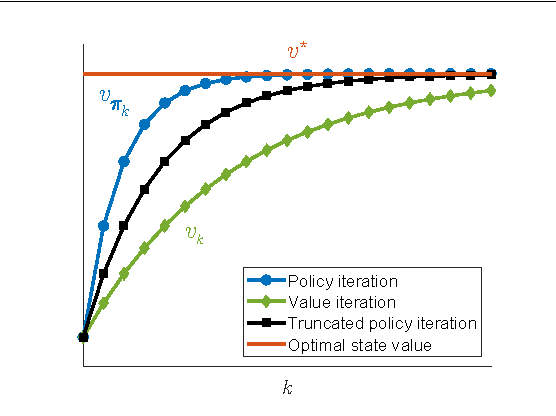
\includegraphics[width=266.8pt]{fig4_5}\par\smallskip
  \begin{minipage}{0.94\textwidth}\footnotesize
  \textbf{Figure 4.5.} An illustration of the relationships between the value iteration, policy iteration, and truncated policy iteration algorithms.\par\smallskip
  \textcolor{rulegray}{\scriptsize Reproduced from S.~Zhao, \emph{Mathematical Foundations of Reinforcement Learning} (Springer, 2025).}
  \end{minipage}
\end{figure}


\subsection{Generalised policy iteration}

\bk{\S4.4, p.~74}

All three algorithms share a shape: alternate a \emph{value} update with a
\emph{policy} update, each making the other better. The book calls this
\textbf{generalised policy iteration (GPI)}, and notes that most RL algorithms in
the book fall under it \bkin{\S4.4, p.~74 and \S4.5 Q\&A, p.~75}. When you meet
Sarsa, Q-learning, DQN and actor-critic later, ask each time: which part is the
value update, and which part is the policy update? You will always find both.

\begin{remark}[``Model-based'' does not mean what you think]
The book is careful here \bkin{\S4.5 Q\&A, pp.~75--76}. The algorithms of this
chapter require the model and are called \emph{dynamic programming}, not
reinforcement learning. The RL terminology is different: \textbf{model-based RL}
means the agent \emph{estimates} a model from data and then plans with it;
\textbf{model-free RL} means no model is ever estimated. Chapters 5--10 are all
model-free.
\end{remark}

\subsection{Chapter 4 self-check}

\begin{enumerate}
  \item In value iteration, are the intermediate $v_k$ state values? In policy
        iteration, are they? Justify both answers.
        \emph{(No / yes; \bkin{\S4.5, p.~74}.)}
  \item Redo the $k=1$ value-iteration table with $\gamma=0.5$ instead of $0.9$.
        Does the greedy policy change?
  \item Explain in one paragraph why policy iteration converges at least as fast as
        value iteration, and why that does not make it strictly better.
  \item Set $j_{\text{truncate}}=1$ in Algorithm 4.3 and show algebraically that you
        recover Algorithm 4.1.
  \item In the $5\times5$ run, why do the far cells acquire correct values last?
\end{enumerate}

\newpage
% ============================================================
\section{Monte Carlo Methods}
% ============================================================

\begin{roadmap}{Chapter 5 of the textbook}
\textbf{Textbook:} Chapter 5, pp.~77--99. Sections: \S5.1 motivating example ---
mean estimation (p.~78; law of large numbers, Box 5.1, p.~80), \S5.2 MC Basic
(p.~80; converting policy iteration to model-free p.~80, the algorithm p.~81,
examples p.~83), \S5.3 MC Exploring Starts (p.~86; using samples efficiently p.~86,
updating policies efficiently p.~87, algorithm p.~88), \S5.4 MC $\varepsilon$-Greedy
(p.~89; $\varepsilon$-greedy policies p.~89, algorithm p.~90, examples p.~91),
\S5.5 exploration versus exploitation (p.~92), \S5.6 summary (p.~97), \S5.7 Q\&A
(p.~97). Algorithms 5.1 (p.~82), 5.2 (p.~88), 5.3 (p.~91).\\[0.3em]
\textbf{Videos:}
\vid{L5 P1 --- Motivating examples}{https://www.youtube.com/watch?v=DO1yXinAV_Q};
\vid{L5 P2 --- MC Basic intro}{https://www.youtube.com/watch?v=6ShisunU0zs};
\vid{L5 P3 --- MC Basic examples}{https://www.youtube.com/watch?v=axA0yns9FxU};
\vid{L5 P4 --- MC Exploring Starts}{https://www.youtube.com/watch?v=Qt8OMHPkLqg};
\vid{L5 P5 --- MC $\varepsilon$-greedy intro}{https://www.youtube.com/watch?v=dM3fYE630pY};
\vid{L5 P6 --- MC $\varepsilon$-greedy examples}{https://www.youtube.com/watch?v=x6X_5ePT9gQ}.\\[0.3em]
\textbf{The turning point of the book.} These are the first \emph{model-free}
algorithms. The author's one-line philosophy \bkin{\S5, p.~77}: ``If we do not have
a model, we must have data. If we do not have data, we must have a model. If we
have neither, we cannot find optimal policies.''
\end{roadmap}

\begin{figure}[htbp]
  \centering
  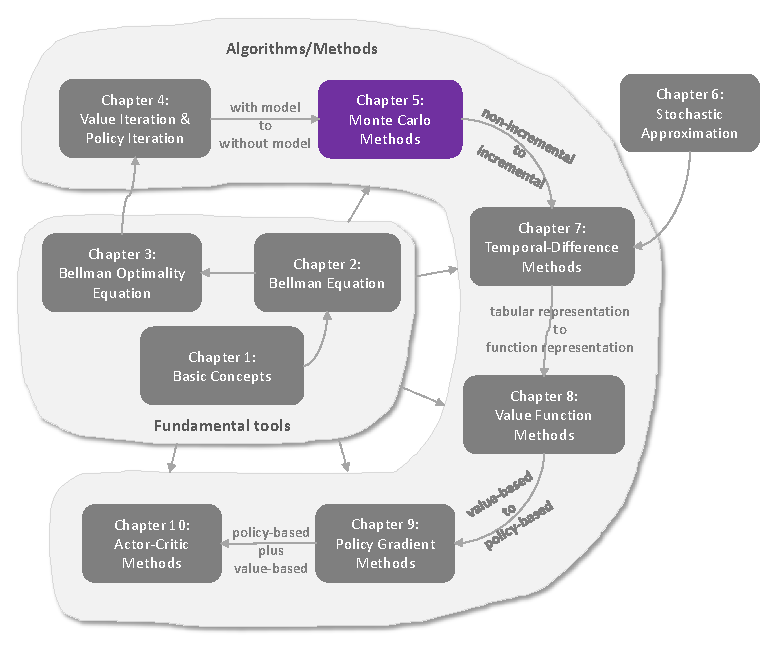
\includegraphics[width=371.3pt]{fig5_1}\par\smallskip
  \begin{minipage}{0.94\textwidth}\footnotesize
  \textbf{Figure 5.1.} Where we are in this book.\par\smallskip
  \textcolor{rulegray}{\scriptsize Reproduced from S.~Zhao, \emph{Mathematical Foundations of Reinforcement Learning} (Springer, 2025).}
  \end{minipage}
\end{figure}


\subsection{Mean estimation: the whole idea in miniature}

\bk{\S5.1, pp.~78--80}

Everything in this chapter rests on one observation: \emph{state and action values
are means}, so estimating them is a mean-estimation problem.

Let $X$ be a random variable taking values in a finite set $\mathcal X$. There are
two ways to get $\E[X]$ \bkin{\S5.1, pp.~78--79}:

\begin{itemize}
  \item \textbf{Model-based:} if you know the distribution,
        $\E[X]=\sum_{x\in\mathcal X}p(x)\,x$.
  \item \textbf{Model-free:} if you do not, draw samples $\{x_1,\dots,x_n\}$ and
        use the sample average $\bar x=\frac1n\sum_{j=1}^n x_j$.
\end{itemize}

\begin{worked}{coin flipping \bkin{\S5.1, p.~79; Figure 5.2, p.~79}}
Let $X=+1$ if heads, $X=-1$ if tails, with $p(X=1)=p(X=-1)=0.5$.

\emph{Model-based:} $\E[X]=0.5(1)+0.5(-1)=0$, computed instantly.

\emph{Model-free:} flip the coin and average. With $n=10$ the average bounces
around; with $n=200$ (the book's Figure 5.2, p.~79) it has visibly settled near
zero. Nobody told the estimator that $p=0.5$; the data did.
\end{worked}

\begin{fact}[Law of large numbers --- Box 5.1, p.~80]
If $\{x_i\}_{i=1}^n$ are i.i.d.\ samples of $X$ and $\bar x=\frac1n\sum_i x_i$, then
\[
  \E[\bar x]=\E[X],\qquad \Var[\bar x]=\frac{\Var[X]}{n}.
\]
So $\bar x$ is \textbf{unbiased}, and its variance vanishes as $n\to\infty$; hence
$\bar x\to\E[X]$.
\end{fact}

\begin{proof}[Proof (Box 5.1, p.~80)]
$\E[\bar x]=\frac1n\sum_i\E[x_i]=\E[X]$ (identical distribution). And
$\Var(\bar x)=\frac{1}{n^2}\sum_i\Var[x_i]=\frac{n\Var[X]}{n^2}=\frac{\Var[X]}{n}$,
where splitting the variance of the sum requires \emph{independence}.
\end{proof}

\begin{warning}[i.i.d.\ is not decoration]
\bkin{\S5.1, p.~79} The book gives the sharp counterexample: if every sample is
forced to equal the first one, the average always equals the first sample no matter
how many you take. Correlated samples can make the estimate useless. Keep this in
mind at \S5.3.1, where the every-visit strategy deliberately introduces some
correlation.
\end{warning}

\begin{figure}[htbp]
  \centering
  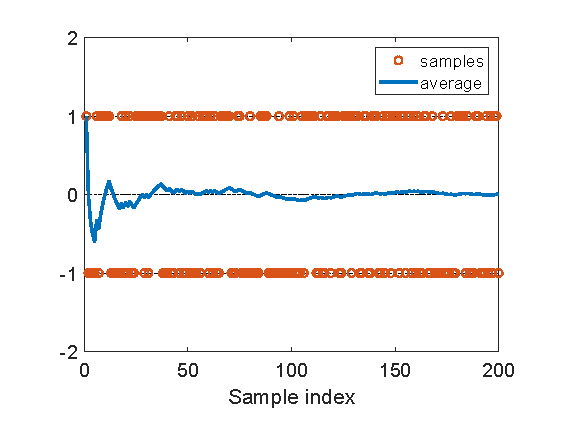
\includegraphics[width=279.4pt]{fig5_2}\par\smallskip
  \begin{minipage}{0.94\textwidth}\footnotesize
  \textbf{Figure 5.2.} An example for demonstrating the law of large numbers. Here, the samples are drawn from \{+1, $-$1\} following a uniform distribution. The average of the samples gradually converges to zero, which is the true expected value, as the number of samples increases.\par\smallskip
  \textcolor{rulegray}{\scriptsize Reproduced from S.~Zhao, \emph{Mathematical Foundations of Reinforcement Learning} (Springer, 2025).}
  \end{minipage}
\end{figure}


\subsection{Making policy iteration model-free}

\bk{\S5.2.1, pp.~80--81; equations (5.1)--(5.2)}

Look at where policy iteration uses the model. In the improvement step,
\[
  \pi_{k+1}(s)=\argmax_\pi\sum_a\pi(a\mid s)\,q_{\pi_k}(s,a),
\]
so \textbf{action values are the only thing that matters}. Policy evaluation exists
solely to produce them. There are two routes to $q_{\pi_k}$
\bkin{\S5.2.1, p.~81}:

\begin{itemize}
  \item \textbf{Model-based} (Chapter 4): solve for $v_{\pi_k}$, then
        \[
          q_{\pi_k}(s,a)=\sum_r p(r\mid s,a)r+\gamma\sum_{s'}p(s'\mid s,a)v_{\pi_k}(s')
          \tag{5.1}
        \]
        --- which needs both halves of the model.
  \item \textbf{Model-free}: recall $q_{\pi_k}(s,a)=\E[G_t\mid S_t=s,A_t=a]$. It is
        a mean. So sample it: run $n$ episodes starting from $(s,a)$ under $\pi_k$,
        record their returns $g^{(i)}_{\pi_k}(s,a)$, and set
        \[
          q_{\pi_k}(s,a)\ \approx\ \frac1n\sum_{i=1}^n g^{(i)}_{\pi_k}(s,a).
          \tag{5.2}
        \]
\end{itemize}

\begin{warning}[Why estimate $q$ and not $v$?]
\bkin{\S5.2.1, p.~82; \S5.7 Q\&A} Because converting $v$ into $q$ requires
equation (5.1), which requires the model. If you are model-free you must estimate
action values \emph{directly}. This is the reason $q$ takes over from $v$ as the
central object for the rest of the book.
\end{warning}

\subsection{MC Basic}

\bk{\S5.2.2, pp.~81--82; Algorithm 5.1, p.~82}

\begin{algobox}{MC Basic (Algorithm 5.1, p.~82)}
\textbf{Input:} an initial policy $\pi_0$. \textbf{No model required.}\\
For $k=0,1,2,\dots$:
\begin{itemize}\itemsep0pt
  \item For every $s\in\Sspace$ and every $a\in\Aspace(s)$:
    \begin{itemize}\itemsep0pt
      \item Collect sufficiently many episodes starting from $(s,a)$, following $\pi_k$.
      \item \textbf{Policy evaluation:} $q_k(s,a)\leftarrow$ the average return of
            those episodes.
    \end{itemize}
  \item \textbf{Policy improvement:} $a_k^*(s)=\argmax_a q_k(s,a)$;
        $\pi_{k+1}(a\mid s)=1$ if $a=a_k^*(s)$, else $0$.
\end{itemize}
\end{algobox}

\begin{remark}
Compare Algorithm 5.1 with Algorithm 4.2 (policy iteration, p.~66). \textbf{The
only difference is one line}: where policy iteration solves the Bellman equation,
MC Basic averages sampled returns. Everything else --- the greedy improvement, the
convergence argument --- is inherited \bkin{\S5.2.2, p.~82}.
\end{remark}

\subsubsection{A hand computation}

\bk{\S5.2.3, pp.~83--84; Figure 5.3, p.~83}

The setting is a $3\times3$ grid with $r_{\text{boundary}}=r_{\text{forbidden}}=-1$,
$r_{\text{target}}=1$, $\gamma=0.9$. The initial policy $\pi_0$ is already optimal
everywhere except $s_1$ and $s_3$.

\begin{worked}{estimating all five action values at $s_1$ \bkin{\S5.2.3, pp.~83--84}}
Because this example is deterministic in both policy and model, running an episode
twice gives the same trajectory --- so \emph{one} episode per $(s,a)$ suffices.

\textbf{$(s_1,a_1)$ --- up, into the wall.} Episode:
$s_1\xrightarrow{a_1}s_1\xrightarrow{a_1}s_1\to\cdots$, rewards $-1,-1,-1,\dots$
\[
  q_{\pi_0}(s_1,a_1)=-1+\gamma(-1)+\gamma^2(-1)+\cdots=\frac{-1}{1-\gamma}=-10 .
\]

\textbf{$(s_1,a_2)$ --- right.} Episode
$s_1\xrightarrow{a_2}s_2\xrightarrow{a_3}s_5\xrightarrow{a_3}\cdots$, rewards
$0,0,0,1,1,\dots$
\[
  q_{\pi_0}(s_1,a_2)=0+\gamma0+\gamma^20+\gamma^3(1)+\gamma^4(1)+\cdots
  =\frac{\gamma^3}{1-\gamma}=\frac{0.729}{0.1}=7.29 .
\]

\textbf{$(s_1,a_3)$ --- down.} Episode
$s_1\xrightarrow{a_3}s_4\xrightarrow{a_2}s_5\xrightarrow{a_3}\cdots$, same reward
pattern:
\[
  q_{\pi_0}(s_1,a_3)=\frac{\gamma^3}{1-\gamma}=7.29 .
\]

\textbf{$(s_1,a_4)$ --- left, into the wall.} As with $a_1$:
$q_{\pi_0}(s_1,a_4)=\frac{-1}{1-\gamma}=-10$.

\textbf{$(s_1,a_5)$ --- stay.} Reward $0$ now, then the policy at $s_1$ bumps the
wall forever:
\[
  q_{\pi_0}(s_1,a_5)=0+\gamma(-1)+\gamma^2(-1)+\cdots=\frac{-\gamma}{1-\gamma}=-9 .
\]

\textbf{Improvement.} The maximum is $7.29$, achieved by both $a_2$ and $a_3$, so
$\pi_1(a_2\mid s_1)=1$ or $\pi_1(a_3\mid s_1)=1$ --- either is optimal. One
iteration was enough here because the policy was already good elsewhere
\bkin{\S5.2.3, p.~84}.
\end{worked}

\begin{figure}[htbp]
  \centering
  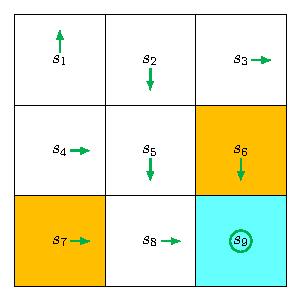
\includegraphics[width=144.3pt]{fig5_3}\par\smallskip
  \begin{minipage}{0.94\textwidth}\footnotesize
  \textbf{Figure 5.3.} An example for illustrating the MC Basic algorithm.\par\smallskip
  \textcolor{rulegray}{\scriptsize Reproduced from S.~Zhao, \emph{Mathematical Foundations of Reinforcement Learning} (Springer, 2025).}
  \end{minipage}
\end{figure}


\subsubsection{Episode length and the sparse-reward problem}

\bk{\S5.2.3, pp.~84--86; Figure 5.4, p.~85}

On a $5\times5$ grid ($r_{\text{boundary}}=-1$, $r_{\text{forbidden}}=-10$,
$r_{\text{target}}=1$, $\gamma=0.9$), the book varies the episode length and shows
the result:

\begin{center}
\small
\begin{tabular}{@{}lp{0.68\textwidth}@{}}
\toprule
Episode length & Outcome \bkin{Figure 5.4, p.~85} \\
\midrule
$1$   & Only cells adjacent to the target have nonzero value ($1.0$); everything else is $0$. \\
$2$   & Values $1.9$ near the target; the frontier of nonzero values expands by one ring. \\
$3,4$ & $2.7$, then $3.4$ near the target; still nothing in the far corners. \\
$14$  & Values everywhere but wrong: row 1 reads $1.2,1.6,2.0,2.5,3.0$. \\
$15$  & The first length at which the bottom-left state can reach the target at all. \\
$30$  & The \emph{policy} is already optimal, though values are still short ($9.6$ at the target instead of $10.0$). \\
$100$ & Both policy and values essentially exact: $3.5,3.9,4.3,4.8,5.3$ in row 1, $10.0$ at the target. \\
\bottomrule
\end{tabular}
\end{center}

\begin{intuition}[The sparse-reward problem]
\bkin{\S5.2.3, p.~86} If a state needs at least $15$ steps to reach the only source
of positive reward, then any episode shorter than $15$ steps returns exactly zero
from that state --- the algorithm receives \emph{no signal at all}. This is the
\textbf{sparse reward} problem, and it is the main practical obstacle in large state
spaces. The standard remedy is reward shaping: hand out small positive rewards near
the target so that an ``attractive field'' guides the agent in
\bkin{\S5.2.3, p.~86}.

Notice, though, the tension with Theorem 3.6: an \emph{affine} change to rewards
changes nothing. Shaping must be \emph{state-dependent} to have any effect.
\end{intuition}

\begin{warning}[Why MC Basic is unusable in practice]
\bkin{\S5.2.2, p.~82} It needs a fresh batch of episodes for \emph{every}
state--action pair in \emph{every} iteration. For a $5\times5$ grid with five
actions that is $125$ batches per iteration. The next two sections are entirely
about fixing this.
\end{warning}

\begin{figure}[htbp]
  \centering
  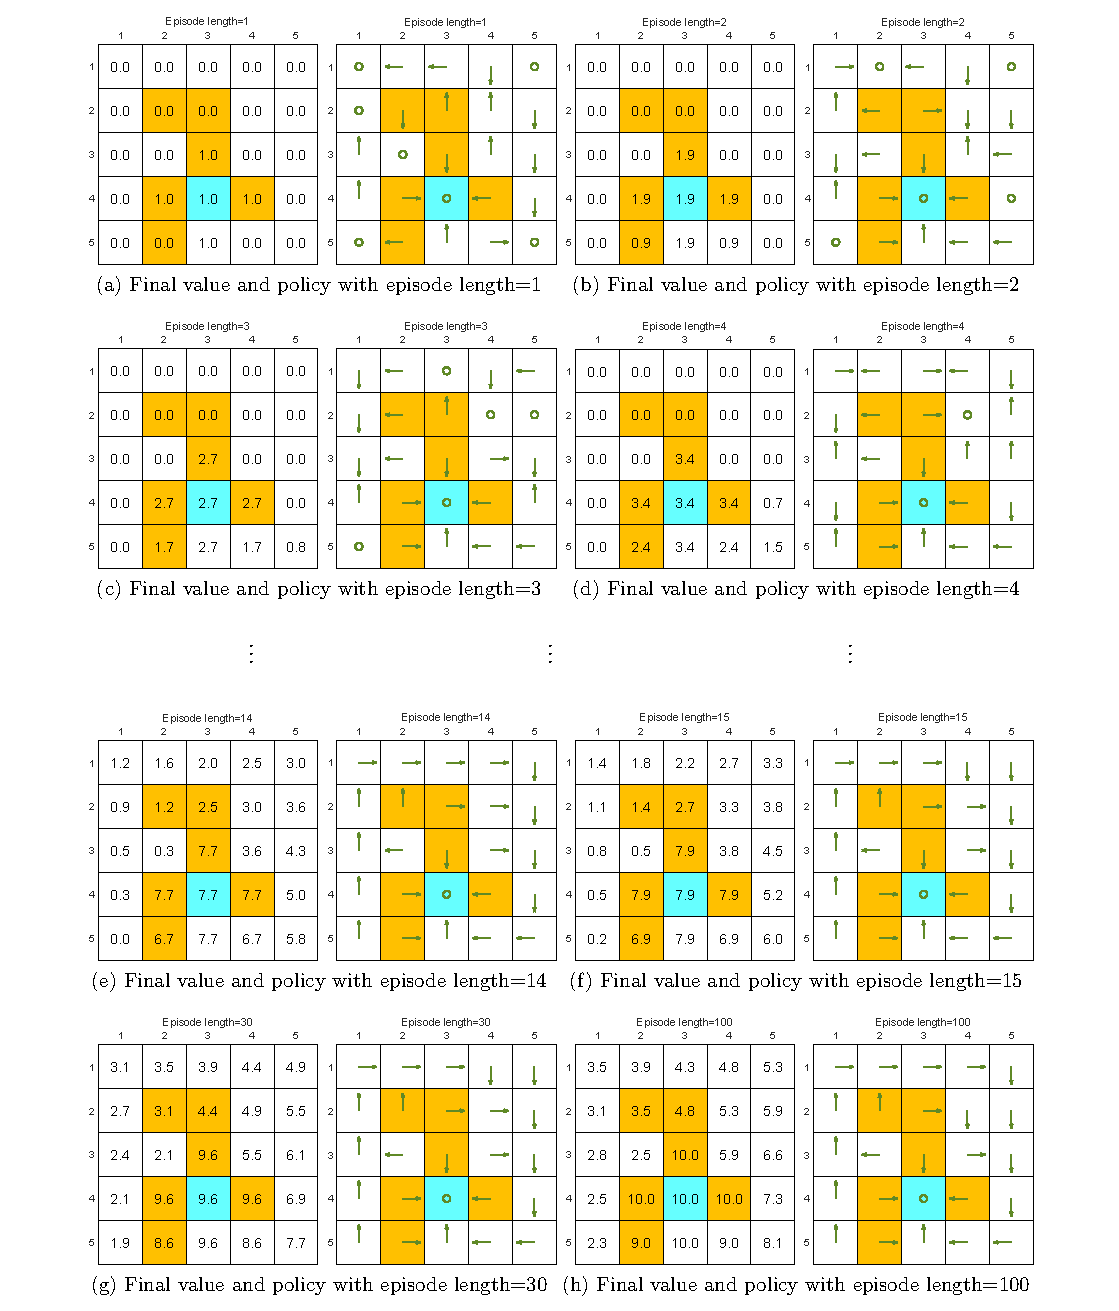
\includegraphics[width=343.8pt]{fig5_4}\par\smallskip
  \begin{minipage}{0.94\textwidth}\footnotesize
  \textbf{Figure 5.4.} The policies and state values obtained by the MC Basic algorithm when given different episode lengths. Only if the length of each episode is sufficiently long, can the state values be accurately estimated.\par\smallskip
  \textcolor{rulegray}{\scriptsize Reproduced from S.~Zhao, \emph{Mathematical Foundations of Reinforcement Learning} (Springer, 2025).}
  \end{minipage}
\end{figure}


\subsection{MC Exploring Starts}

\bk{\S5.3, pp.~86--89; Algorithm 5.2, p.~88}

Two independent efficiency ideas.

\subsubsection{Idea 1: reuse every visit in an episode}

\bk{\S5.3.1, pp.~86--87; equation (5.3)}

Suppose an episode under $\pi$ is
\[
  s_1\xrightarrow{a_2}s_2\xrightarrow{a_4}s_1\xrightarrow{a_2}s_2
  \xrightarrow{a_3}s_5\xrightarrow{a_1}\cdots
  \tag{5.3}
\]
MC Basic uses this episode to estimate only $q(s_1,a_2)$ --- the
\textbf{initial-visit} strategy. But the tail of the episode after any visit is
itself a valid episode:
\[
\begin{aligned}
  s_1\xrightarrow{a_2}s_2\xrightarrow{a_4}s_1\xrightarrow{a_2}s_2\xrightarrow{a_3}s_5\xrightarrow{a_1}\cdots
  &\quad\text{[original: estimates }q(s_1,a_2)]\\
  s_2\xrightarrow{a_4}s_1\xrightarrow{a_2}s_2\xrightarrow{a_3}s_5\xrightarrow{a_1}\cdots
  &\quad\text{[estimates }q(s_2,a_4)]\\
  s_1\xrightarrow{a_2}s_2\xrightarrow{a_3}s_5\xrightarrow{a_1}\cdots
  &\quad\text{[estimates }q(s_1,a_2)\text{ again]}\\
  s_2\xrightarrow{a_3}s_5\xrightarrow{a_1}\cdots
  &\quad\text{[estimates }q(s_2,a_3)]\\
  s_5\xrightarrow{a_1}\cdots
  &\quad\text{[estimates }q(s_5,a_1)]
\end{aligned}
\]
Three strategies \bkin{\S5.3.1, p.~87; \S5.7 Q\&A, p.~98}:
\begin{itemize}
  \item \textbf{initial-visit}: use the episode only for its starting pair (MC Basic);
  \item \textbf{first-visit}: use each pair the first time it appears;
  \item \textbf{every-visit}: use each pair every time it appears.
\end{itemize}
Every-visit squeezes the most out of the data. The price: the sub-episode starting
at the second visit to $(s_1,a_2)$ is a \emph{subset} of the one starting at the
first, so the returns are correlated --- the i.i.d.\ assumption is bent. The book's
verdict: the correlation is weak if the two visits are far apart in the trajectory
\bkin{\S5.3.1, p.~87}.

\subsubsection{Idea 2: update the policy after every episode}

\bk{\S5.3.2, pp.~87--88}

MC Basic waits until all episodes for a pair have been collected before touching
the policy. Instead, use the return from a \emph{single} episode as a rough
estimate and improve immediately. The estimate is noisy, but this is just
generalised policy iteration: you may update the policy before the value estimate
has converged \bkin{\S5.3.2, p.~88; \S4.4, p.~74}.

\begin{algobox}{MC Exploring Starts (Algorithm 5.2, p.~88)}
\textbf{Initialise:} $\pi_0(a\mid s)$ and $q(s,a)$ for all $(s,a)$;
$\mathrm{Returns}(s,a)=0$ and $\mathrm{Num}(s,a)=0$.\\
For each episode:
\begin{itemize}\itemsep0pt
  \item \textbf{Episode generation.} Choose a starting pair $(s_0,a_0)$, ensuring
        every pair can be chosen (\emph{this is the exploring-starts condition}).
        Follow $\pi$ to generate $s_0,a_0,r_1,\dots,s_{T-1},a_{T-1},r_T$.
  \item Set $g\leftarrow 0$. For $t=T-1,T-2,\dots,0$:
    \begin{itemize}\itemsep0pt
      \item $g\leftarrow \gamma g + r_{t+1}$
      \item $\mathrm{Returns}(s_t,a_t)\leftarrow \mathrm{Returns}(s_t,a_t)+g$;\quad
            $\mathrm{Num}(s_t,a_t)\leftarrow \mathrm{Num}(s_t,a_t)+1$
      \item \textbf{Evaluation:} $q(s_t,a_t)\leftarrow \mathrm{Returns}(s_t,a_t)/\mathrm{Num}(s_t,a_t)$
      \item \textbf{Improvement:} $\pi(a\mid s_t)=1$ if $a=\argmax_{a'}q(s_t,a')$, else $0$
    \end{itemize}
\end{itemize}
\end{algobox}

\begin{remark}[Why the loop runs backwards]
\bkin{\S5.3.3, p.~88} The recursion $g\leftarrow\gamma g+r_{t+1}$ computes every
suffix return in a single backward pass, in $O(T)$ total time instead of $O(T^2)$.
It is exactly the bootstrapping identity $G_t=R_{t+1}+\gamma G_{t+1}$ used as a
computational device.
\end{remark}

\begin{warning}[The exploring-starts condition]
\bkin{\S5.3.3, p.~89; \S5.7 Q\&A, p.~98} The algorithm requires enough episodes
starting from \emph{every} state--action pair. In theory this is necessary: if some
action is never tried, its value is never estimated, and the greedy policy may
never select it even though it is the best. In practice it is often impossible ---
you cannot reset a physical robot into an arbitrary state and force an arbitrary
first action. The next section removes the condition.
\end{warning}

\subsection{MC $\varepsilon$-Greedy}

\bk{\S5.4, pp.~89--92; Algorithm 5.3, p.~91}

\subsubsection{$\varepsilon$-greedy policies}

\bk{\S5.4.1, pp.~89--90}

A policy is \textbf{soft} if every action has positive probability at every state.
A single sufficiently long episode generated by a soft policy will visit every
state--action pair many times --- which is precisely what exploring starts was
trying to buy.

\begin{definition}[$\varepsilon$-greedy policy]
For $\varepsilon\in[0,1]$,
\[
  \pi(a\mid s)=
  \begin{cases}
    1-\dfrac{\varepsilon}{|\Aspace(s)|}\bigl(|\Aspace(s)|-1\bigr), & \text{for the greedy action},\\[0.9em]
    \dfrac{\varepsilon}{|\Aspace(s)|}, & \text{for each of the other } |\Aspace(s)|-1 \text{ actions}.
  \end{cases}
\]
\end{definition}

\begin{worked}{concrete probabilities with $|\Aspace|=5$}
\[
\begin{array}{llll}
\varepsilon=0:   & \text{greedy action } 1.00, & \text{others } 0.00 & \text{(pure greedy)}\\
\varepsilon=0.1: & 1-\tfrac{0.1}{5}(4)=0.92,   & \tfrac{0.1}{5}=0.02 & \\
\varepsilon=0.5: & 1-\tfrac{0.5}{5}(4)=0.60,   & \tfrac{0.5}{5}=0.10 & \\
\varepsilon=1:   & 0.20,                        & 0.20                & \text{(uniform)}
\end{array}
\]
Check: $0.6+4(0.1)=1$. \checkmark
\end{worked}

The greedy action always keeps the largest probability, since
\[
  1-\frac{\varepsilon}{|\Aspace|}(|\Aspace|-1)=1-\varepsilon+\frac{\varepsilon}{|\Aspace|}
  \ \ge\ \frac{\varepsilon}{|\Aspace|}
  \qquad\text{for all }\varepsilon\in[0,1]
\]
\bkin{\S5.4.1, p.~90}. Implementation: draw $x\sim U[0,1]$; if $x\ge\varepsilon$
take the greedy action, otherwise pick uniformly at random from $\Aspace(s)$ ---
which may re-select the greedy action, which is why the total greedy probability is
$1-\varepsilon+\varepsilon/|\Aspace|$ \bkin{\S5.4.1, p.~90}.

\subsubsection{The algorithm}

\bk{\S5.4.2, pp.~90--91; equations (5.4)--(5.5)}

The only change is in the improvement step. Instead of
\[
  \pi_{k+1}(s)=\argmax_{\pi\in\Pi}\sum_a\pi(a\mid s)q_{\pi_k}(s,a)
  \tag{5.4}
\]
over \emph{all} policies $\Pi$, we optimise over $\Pi_\varepsilon$, the set of
$\varepsilon$-greedy policies with that fixed $\varepsilon$:
\[
  \pi_{k+1}(s)=\argmax_{\pi\in\Pi_\varepsilon}\sum_a\pi(a\mid s)q_{\pi_k}(s,a),
  \tag{5.5}
\]
whose solution is the $\varepsilon$-greedy policy centred on
$a_k^*=\argmax_a q_{\pi_k}(s,a)$.

\begin{algobox}{MC $\varepsilon$-Greedy (Algorithm 5.3, p.~91)}
\textbf{Initialise:} $\pi_0$, $q(s,a)$, $\mathrm{Returns}(s,a)=0$,
$\mathrm{Num}(s,a)=0$, and $\varepsilon\in(0,1]$.\\
For each episode:
\begin{itemize}\itemsep0pt
  \item Choose \emph{any} starting pair $(s_0,a_0)$ --- \textbf{exploring starts is
        no longer required} --- and follow $\pi$ for $T$ steps.
  \item $g\leftarrow0$. For $t=T-1,\dots,0$:
    \begin{itemize}\itemsep0pt
      \item $g\leftarrow\gamma g+r_{t+1}$;\quad
            $\mathrm{Returns}(s_t,a_t)\mathrel{+}=g$;\quad
            $\mathrm{Num}(s_t,a_t)\mathrel{+}=1$
      \item $q(s_t,a_t)\leftarrow\mathrm{Returns}(s_t,a_t)/\mathrm{Num}(s_t,a_t)$
      \item With $a^*=\argmax_a q(s_t,a)$, set
            $\pi(a\mid s_t)=1-\frac{\varepsilon}{|\Aspace(s_t)|}(|\Aspace(s_t)|-1)$
            if $a=a^*$, and $\frac{\varepsilon}{|\Aspace(s_t)|}$ otherwise.
    \end{itemize}
\end{itemize}
\end{algobox}

\begin{warning}[In what sense is the result optimal?]
\bkin{\S5.4.2, p.~91; \S5.7 Q\&A, p.~98} Yes and no. \emph{Yes}: with enough samples
the algorithm converges to the best policy \textbf{within $\Pi_\varepsilon$}.
\emph{No}: that is generally not the best policy within $\Pi$. If $\varepsilon$ is
small the two are close; if $\varepsilon$ is large they are not, as the numbers
below show.
\end{warning}

\subsubsection{Learning from a single very long episode}

\bk{\S5.4.3, pp.~91--92; Figure 5.5, p.~92}

The book runs MC $\varepsilon$-Greedy with $\varepsilon=0.5$ using \emph{one}
episode of one million steps per iteration, starting from the uniform policy
($0.2$ on every action), with $r_{\text{boundary}}=r_{\text{forbidden}}=-1$,
$r_{\text{target}}=1$, $\gamma=0.9$. The optimal $\varepsilon$-greedy policy is
reached after \textbf{two iterations} \bkin{\S5.4.3, p.~91}. One episode suffices
because the soft policy visits every state--action pair many times.

\begin{figure}[htbp]
  \centering
  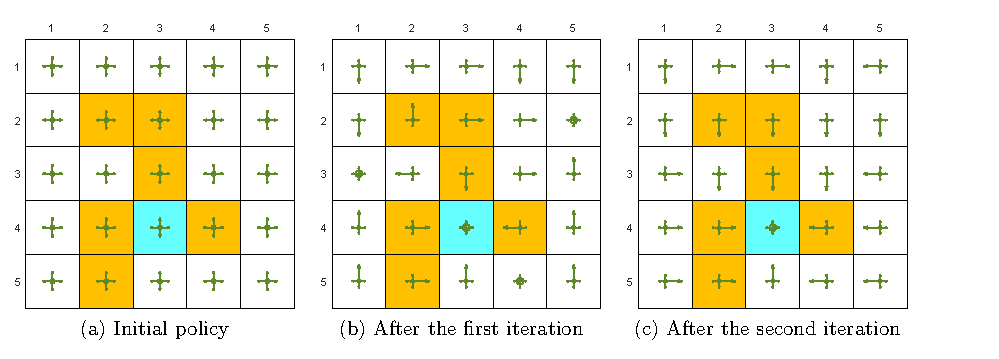
\includegraphics[width=441.6pt]{fig5_5}\par\smallskip
  \begin{minipage}{0.94\textwidth}\footnotesize
  \textbf{Figure 5.5.} The evolution process of the MC $\varepsilon$-Greedy algorithm based on single episodes.\par\smallskip
  \textcolor{rulegray}{\scriptsize Reproduced from S.~Zhao, \emph{Mathematical Foundations of Reinforcement Learning} (Springer, 2025).}
  \end{minipage}
\end{figure}


\subsection{Exploration versus exploitation, quantified}

\bk{\S5.5, pp.~92--97; Figures 5.6--5.8, pp.~93--96}

\begin{definition}
\textbf{Exploration} means trying as many actions as possible so that every action
value is well estimated. \textbf{Exploitation} means taking the action that
currently looks best. They pull in opposite directions, because the current
estimates may be wrong precisely where you have not explored.
\end{definition}

The book measures the trade-off on a $5\times5$ grid
($r_{\text{boundary}}=-1$, $r_{\text{forbidden}}=-10$, $r_{\text{target}}=1$,
$\gamma=0.9$).

\begin{worked}{cost of exploration: state values collapse as $\varepsilon$ grows \bkin{Figure 5.6, p.~93}}
Take a fixed set of ``consistent'' $\varepsilon$-greedy policies (same action has
the largest probability in each) and evaluate them:
\[
\begin{array}{ll}
\varepsilon=0:   & \text{row 1} = 3.5,\ 3.9,\ 4.3,\ 4.8,\ 5.3;\quad \text{target cell}=10.0\\
\varepsilon=0.1: & \text{row 1} = 0.4,\ 0.5,\ 0.9,\ 1.3,\ 1.4;\quad \text{target cell}=3.4\\
\varepsilon=0.2: & \text{row 1} = -2.2,\ -2.4,\ -2.1,\ -1.7,\ -1.8\\
\varepsilon=0.5: & \text{row 1} = -8.0,\ -9.0,\ -8.4,\ -7.2,\ -7.8;\ \text{worst cell}=-17.0
\end{array}
\]
The values do not merely decline --- they go sharply negative. The book explains
why the \emph{target} cell suffers most \bkin{\S5.5, p.~95}: with $\varepsilon$
large, an agent sitting on the target keeps randomly wandering into the
surrounding forbidden cells and eating $-10$.
\end{worked}

\begin{figure}[htbp]
  \centering
  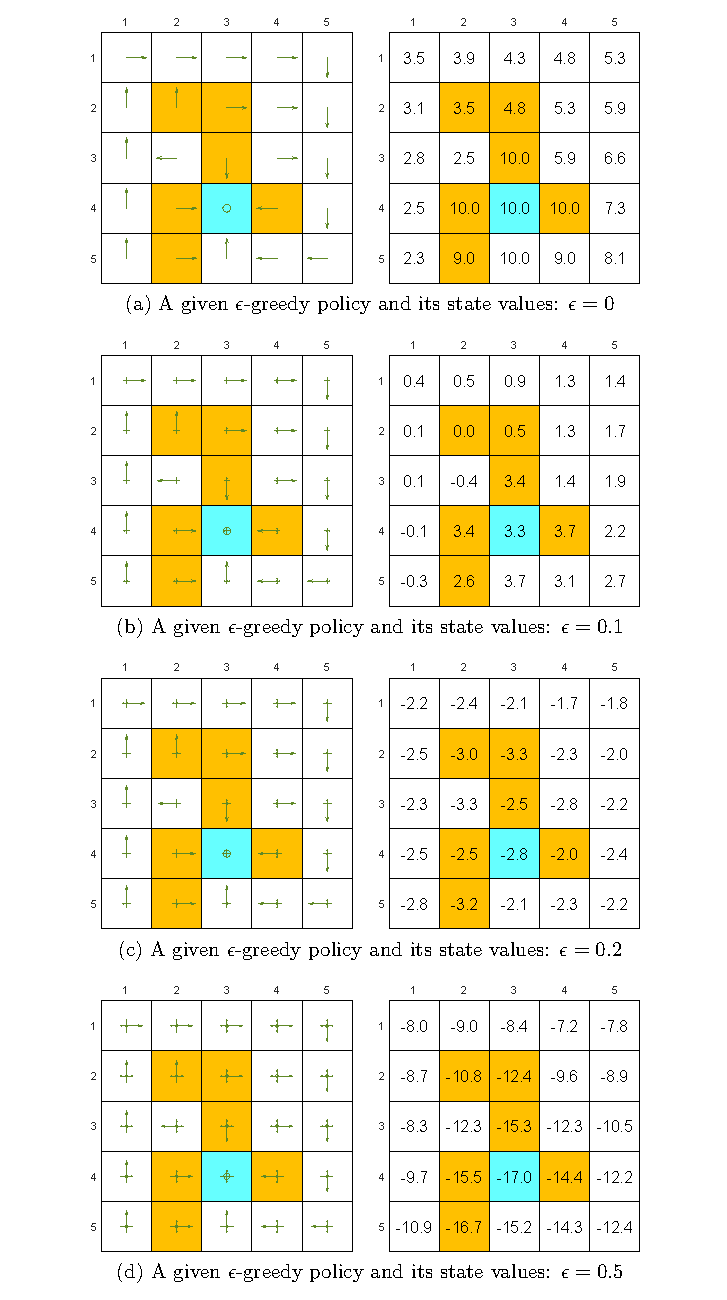
\includegraphics[width=225.4pt]{fig5_6}\par\smallskip
  \begin{minipage}{0.94\textwidth}\footnotesize
  \textbf{Figure 5.6.} The state values of some $\varepsilon$-greedy policies. These $\varepsilon$-greedy policies are consistent with each other in the sense that the actions with the greatest probabilities are the same. It can be seen that, when the value of $\varepsilon$ increases, the state values of the $\varepsilon$-greedy policies decrease and hence their optimality becomes worse.\par\smallskip
  \textcolor{rulegray}{\scriptsize Reproduced from S.~Zhao, \emph{Mathematical Foundations of Reinforcement Learning} (Springer, 2025).}
  \end{minipage}
\end{figure}


\begin{worked}{when does exploration change the answer? \bkin{Figure 5.7, p.~94}}
Now compute the policy that is \emph{optimal within} $\Pi_\varepsilon$:
\begin{itemize}
  \item $\varepsilon=0$: the greedy optimal policy; values $3.5,\dots,10.0$.
  \item $\varepsilon=0.1$: the optimal $\varepsilon$-greedy policy is
        \emph{consistent} with the greedy optimal one --- same arrows, lower values
        ($0.4,0.5,0.9,1.3,1.4$ in row 1).
  \item $\varepsilon=0.2$: consistency \textbf{breaks}. The optimal
        $\varepsilon$-greedy policy now points differently from the greedy optimum.
  \item $\varepsilon=0.5$: badly inconsistent; values around $-4$ to $-10$.
\end{itemize}
\textbf{Rule of thumb:} keep $\varepsilon$ small enough that the optimal
$\varepsilon$-greedy policy still agrees with the greedy optimum
\bkin{\S5.5, p.~95}.
\end{worked}

\begin{figure}[htbp]
  \centering
  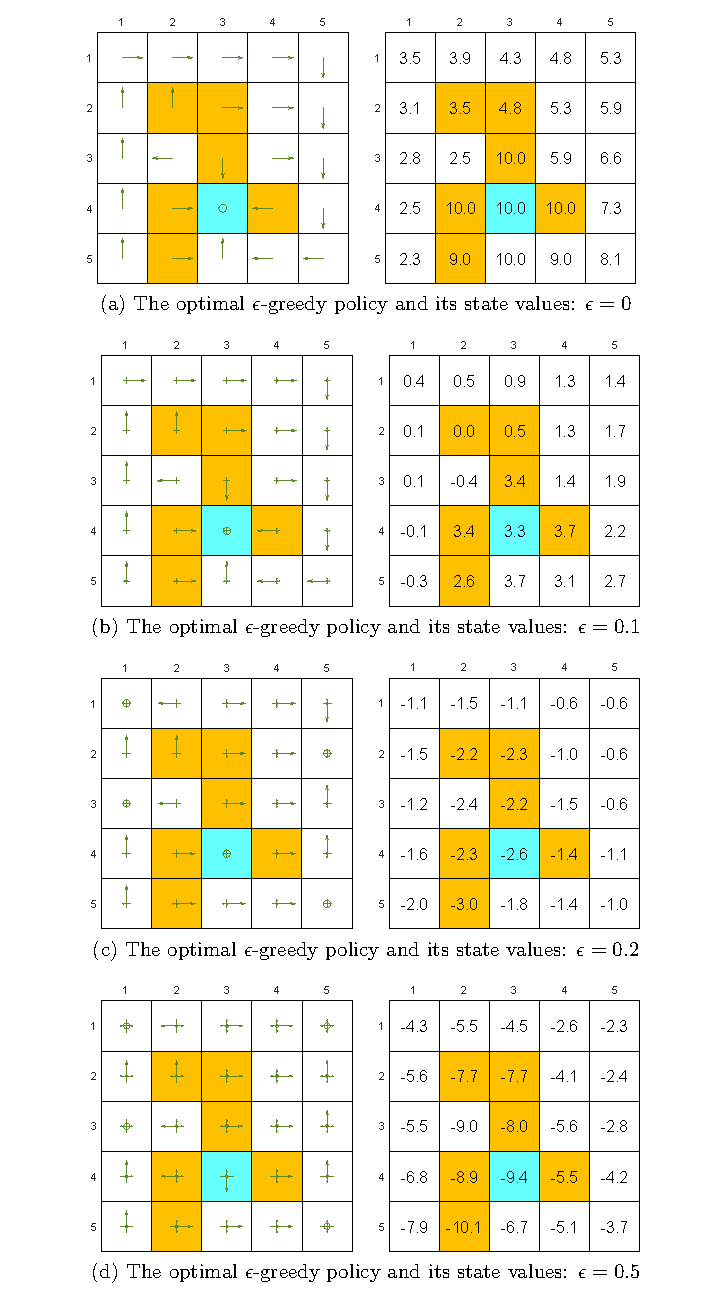
\includegraphics[width=225.4pt]{fig5_7}\par\smallskip
  \begin{minipage}{0.94\textwidth}\footnotesize
  \textbf{Figure 5.7.} The optimal $\varepsilon$-greedy policies and their corresponding state values under different values of $\varepsilon$. Here, these $\varepsilon$-greedy policies are optimal among all $\varepsilon$-greedy ones (with the same value of $\varepsilon$). It can be seen that, when the value of $\varepsilon$ increases, the optimal $\varepsilon$-greedy policies are no longer consistent with the optimal one as in (a).\par\smallskip
  \textcolor{rulegray}{\scriptsize Reproduced from S.~Zhao, \emph{Mathematical Foundations of Reinforcement Learning} (Springer, 2025).}
  \end{minipage}
\end{figure}


\begin{worked}{benefit of exploration: coverage \bkin{Figure 5.8, p.~96}}
Count how often each of the $125$ state--action pairs is visited in a single
episode of one million steps:
\begin{itemize}
  \item $\varepsilon=1$ (uniform): every pair is visited roughly
        $7600$--$8300$ times --- almost perfectly even coverage.
  \item $\varepsilon=0.5$: wildly uneven. Some pairs are visited more than
        $250{,}000$ times while most receive only hundreds or even tens of visits.
\end{itemize}
So the exploration benefit is real and it degrades fast as $\varepsilon$ falls.
\end{worked}

\begin{intuition}[The standard resolution]
\bkin{\S5.5, p.~97} Start with $\varepsilon$ large to explore, then \emph{decay} it
toward zero so that the final policy is (nearly) greedy and therefore (nearly)
optimal. You get coverage early and optimality late. Every practical
implementation --- including DQN in Chapter 8 --- does some version of this.
\end{intuition}

\begin{figure}[htbp]
  \centering
  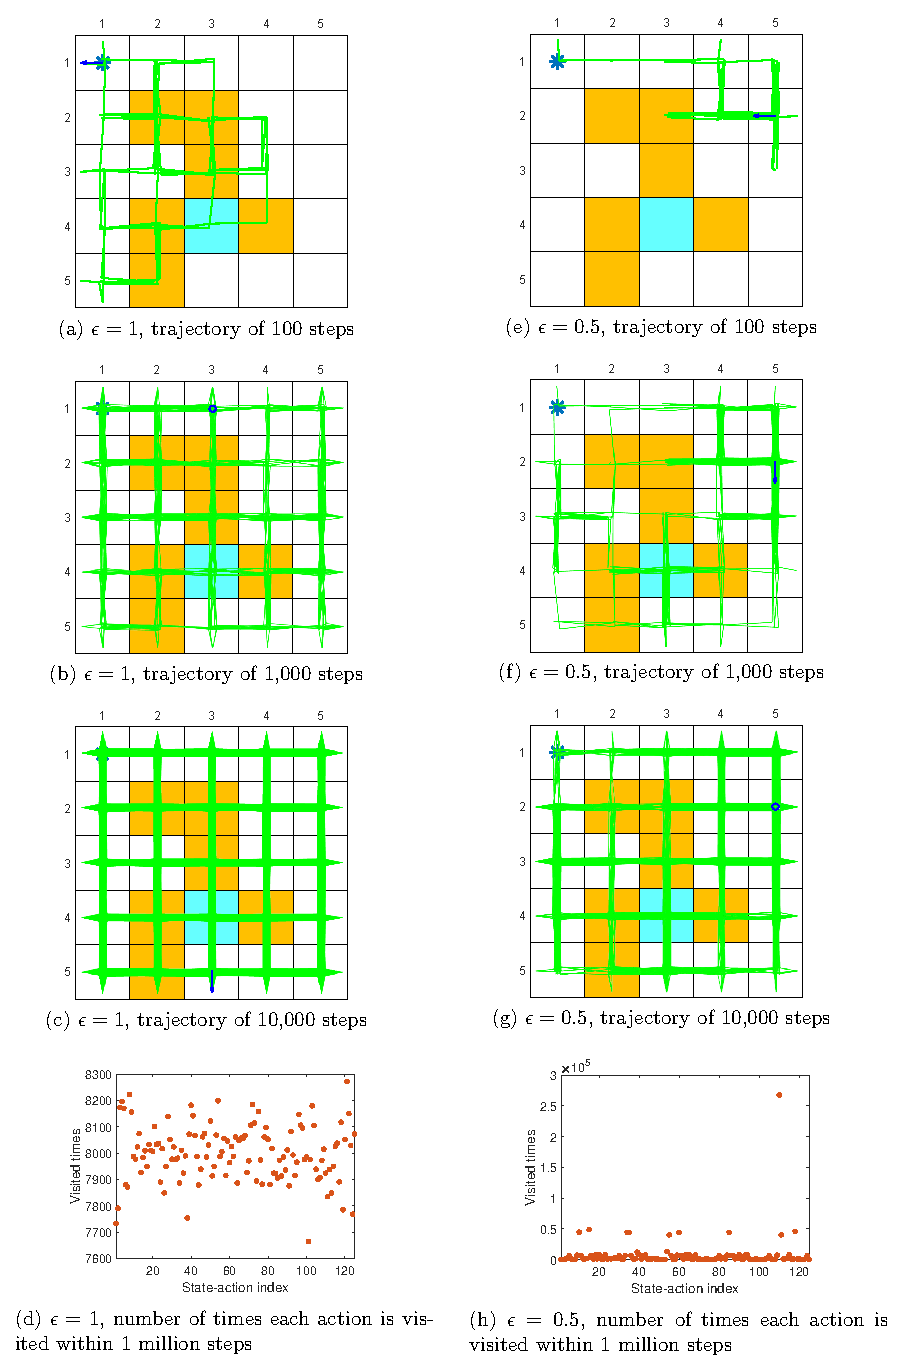
\includegraphics[width=265.5pt]{fig5_8}\par\smallskip
  \begin{minipage}{0.94\textwidth}\footnotesize
  \textbf{Figure 5.8.} Exploration abilities of $\varepsilon$-greedy policies with different values of $\varepsilon$.\par\smallskip
  \textcolor{rulegray}{\scriptsize Reproduced from S.~Zhao, \emph{Mathematical Foundations of Reinforcement Learning} (Springer, 2025).}
  \end{minipage}
\end{figure}


\subsection{Summary and self-check}

\bk{\S5.6, p.~97}

\begin{center}
\small
\begin{tabular}{@{}lp{0.62\textwidth}@{}}
\toprule
Algorithm & What it changes \\
\midrule
MC Basic & Policy iteration with sampled returns replacing the model in the evaluation step. Correct but hopelessly sample-inefficient. \\
MC Exploring Starts & Adds first-visit / every-visit sample reuse and episode-by-episode policy updates. Still needs exploring starts. \\
MC $\varepsilon$-Greedy & Optimises over $\Pi_\varepsilon$ instead of $\Pi$ in the improvement step. Soft policies supply exploration, so exploring starts is dropped; the price is optimality within $\Pi_\varepsilon$ only. \\
\bottomrule
\end{tabular}
\end{center}

\begin{enumerate}
  \item Why is a model-free algorithm forced to estimate $q_\pi$ rather than
        $v_\pi$? \emph{(Equation (5.1) needs the model.)}
  \item Recompute $q_{\pi_0}(s_1,a_5)=-\gamma/(1-\gamma)$ from scratch with
        $\gamma=0.5$ and explain the sign.
  \item Distinguish initial-visit, first-visit and every-visit, and say which one
        risks violating the i.i.d.\ assumption.
  \item Give one theoretical and one practical reason the exploring-starts
        condition is unattractive.
  \item With $|\Aspace|=5$ and $\varepsilon=0.4$, write out all five probabilities
        and check that they sum to one.
  \item Explain why increasing $\varepsilon$ lowers the value of the \emph{target}
        state more than that of a far-away state. \emph{(\bkin{\S5.5, p.~95}.)}
\end{enumerate}

\newpage
% ============================================================
\section{Stochastic Approximation}
% ============================================================

\begin{roadmap}{Chapter 6 of the textbook}
\textbf{Textbook:} Chapter 6, pp.~101--124. Sections: \S6.1 motivating example ---
mean estimation (p.~102), \S6.2 Robbins--Monro algorithm (p.~103; convergence
properties p.~105, application to mean estimation p.~108), \S6.3 Dvoretzky's
convergence theorem (p.~109; proof p.~110, applications pp.~112--113, extension
p.~113), \S6.4 stochastic gradient descent (p.~114; mean estimation p.~116,
convergence pattern p.~116, deterministic formulation p.~118, BGD/SGD/MBGD p.~119,
convergence of SGD p.~121), \S6.5 summary (p.~123), \S6.6 Q\&A (p.~123).\\[0.3em]
\textbf{Videos:}
\vid{L6 P1 --- Motivating example}{https://www.youtube.com/watch?v=1bMgejvWoAo};
\vid{L6 P2 --- RM: introduction}{https://www.youtube.com/watch?v=1FTGcNUUnCE};
\vid{L6 P3 --- RM: convergence}{https://www.youtube.com/watch?v=juNDoAFEre4};
\vid{L6 P4 --- SGD: introduction}{https://www.youtube.com/watch?v=EZO7Iadp5m4};
\vid{L6 P5 --- SGD: examples}{https://www.youtube.com/watch?v=BsxU_4qvvNA};
\vid{L6 P6 --- SGD: properties}{https://www.youtube.com/watch?v=fWxX9YuEHjE};
\vid{L6 P7 --- SGD: comparison}{https://www.youtube.com/watch?v=yNEV2cLKuzU}.\\[0.3em]
\textbf{Why this chapter exists.} It introduces no RL algorithm at all. It exists to
close a gap: everything so far has been \emph{non-incremental} (collect all the
data, then compute), and everything from Chapter 7 onward is \emph{incremental}
(update after every single observation). Without this chapter the
temporal-difference update in Chapter 7 looks like it fell out of the sky
\bkin{\S6, pp.~101--102}.
\end{roadmap}

\begin{figure}[htbp]
  \centering
  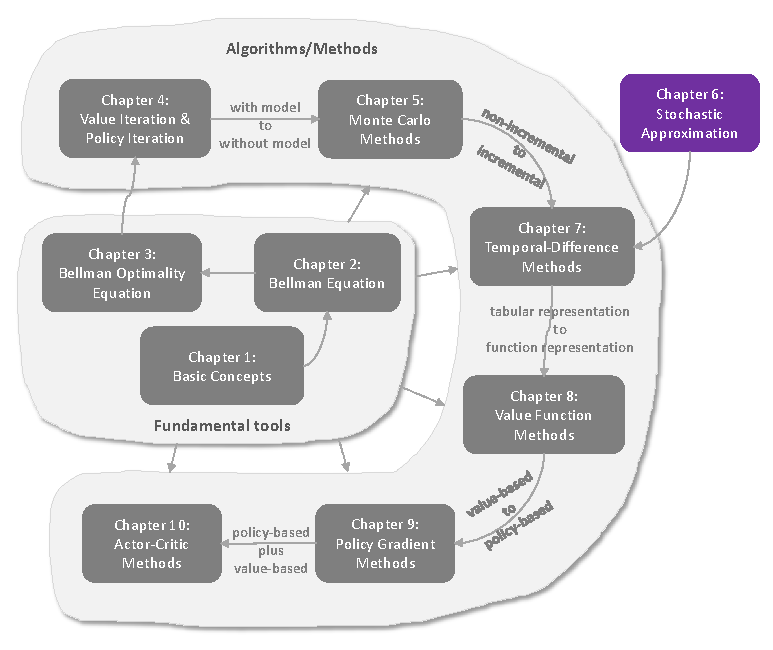
\includegraphics[width=371.3pt]{fig6_1}\par\smallskip
  \begin{minipage}{0.94\textwidth}\footnotesize
  \textbf{Figure 6.1.} Where we are in this book.\par\smallskip
  \textcolor{rulegray}{\scriptsize Reproduced from S.~Zhao, \emph{Mathematical Foundations of Reinforcement Learning} (Springer, 2025).}
  \end{minipage}
\end{figure}


\subsection{From batch to incremental: mean estimation again}

\bk{\S6.1, pp.~102--103; equations (6.1)--(6.4)}

We want $\E[X]$ from i.i.d.\ samples $\{x_i\}$. The batch estimator is
$\bar x=\frac1n\sum_{i=1}^n x_i$ \bkin{equation (6.1), p.~102}. Its drawback: you
must wait for all $n$ samples before you have any answer at all.

Define $w_{k+1}=\frac1k\sum_{i=1}^k x_i$, so that $w_k=\frac{1}{k-1}\sum_{i=1}^{k-1}x_i$.
Then \bkin{\S6.1, p.~102}
\[
  w_{k+1}=\frac1k\sum_{i=1}^k x_i
  =\frac1k\Bigl(\sum_{i=1}^{k-1}x_i+x_k\Bigr)
  =\frac1k\bigl((k-1)w_k+x_k\bigr)
  = w_k-\frac1k(w_k-x_k).
\]

\begin{definition}[Incremental mean estimation, equation (6.2), p.~103]
\[
  \boxed{\;w_{k+1}=w_k-\frac1k\bigl(w_k-x_k\bigr).\;}
\]
\end{definition}

\begin{worked}{unrolling the recursion \bkin{equation (6.3), p.~103}}
\[
\begin{aligned}
  w_1&=x_1,\\
  w_2&=w_1-\tfrac11(w_1-x_1)=x_1,\\
  w_3&=w_2-\tfrac12(w_2-x_2)=x_1-\tfrac12(x_1-x_2)=\tfrac12(x_1+x_2),\\
  w_4&=w_3-\tfrac13(w_3-x_3)=\tfrac13(x_1+x_2+x_3),\\
     &\ \ \vdots\\
  w_{k+1}&=\tfrac1k\textstyle\sum_{i=1}^k x_i .
\end{aligned}
\]
So the incremental form is \emph{exactly} the running average --- no approximation
anywhere. It merely lets you read off an answer at every step instead of only at the
end \bkin{\S6.1, p.~103}.
\end{worked}

\begin{intuition}[Read the update as an error correction]
Write $w_{k+1}=w_k-\alpha_k(w_k-x_k)$. The bracket $(w_k-x_k)$ is
``what I currently believe minus what I just saw'' --- a prediction error. The
update nudges the belief \emph{against} the error, by a fraction $\alpha_k$. Every
learning rule for the rest of this book has this shape:
\[
  \text{new estimate} \;=\; \text{old estimate} \;-\; \text{step size}\times\text{error}.
\]
Chapter 7's TD update, Chapter 8's gradient update and Chapter 10's actor update
are all instances.
\end{intuition}

Now generalise the coefficient \bkin{equation (6.4), p.~103}:
\[
  w_{k+1}=w_k-\alpha_k(w_k-x_k).
\]
With $\alpha_k=1/k$ we recover the exact average. With a general $\alpha_k$ there is
no closed form --- so we need a theory that tells us when this still converges.
That theory is stochastic approximation.

\subsection{The Robbins--Monro algorithm}

\bk{\S6.2, pp.~103--105; Figures 6.2--6.3, pp.~104--105}

\textbf{The problem.} Find the root of $g(w)=0$, where $g:\R\to\R$, when

\begin{itemize}
  \item you do \emph{not} know the expression of $g$,
  \item you do \emph{not} know its derivative,
  \item and you can only obtain \emph{noisy} evaluations
        $\tilde g(w,\eta)=g(w)+\eta$ at inputs $w$ of your choosing.
\end{itemize}

It is a black box \bkin{Figure 6.2, p.~104}. Note that this covers optimisation too:
minimising $J(w)$ is finding the root of $g(w)\doteq\nabla_wJ(w)=0$, and solving
$g(w)=c$ is finding the root of $g(w)-c$ \bkin{\S6.2, p.~104}.

\begin{definition}[Robbins--Monro algorithm, equation (6.5), p.~104]
\[
  \boxed{\;w_{k+1}=w_k-a_k\,\tilde g(w_k,\eta_k),\qquad k=1,2,3,\dots\;}
\]
\end{definition}

That is the entire algorithm. No gradients, no function evaluations other than the
noisy output.

\begin{figure}[htbp]
  \centering
  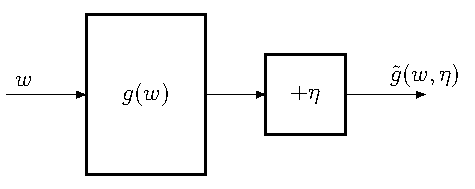
\includegraphics[width=228.1pt]{fig6_2}\par\smallskip
  \begin{minipage}{0.94\textwidth}\footnotesize
  \textbf{Figure 6.2.} An illustration of the problem of solving g(w) = 0 from w and \~\{\}g.\par\smallskip
  \textcolor{rulegray}{\scriptsize Reproduced from S.~Zhao, \emph{Mathematical Foundations of Reinforcement Learning} (Springer, 2025).}
  \end{minipage}
\end{figure}


\begin{worked}{RM in action \bkin{Figure 6.3, p.~105}}
Take $g(w)=w^3-5$, whose true root is $5^{1/3}\approx1.71$. We may observe only
$\tilde g(w)=g(w)+\eta$ with $\eta\sim N(0,1)$ i.i.d. Start at $w_1=0$ with
$a_k=1/k$. Despite every observation being corrupted by standard normal noise,
$w_k$ converges to $1.71$ within about $50$ iterations.
\end{worked}

\begin{figure}[htbp]
  \centering
  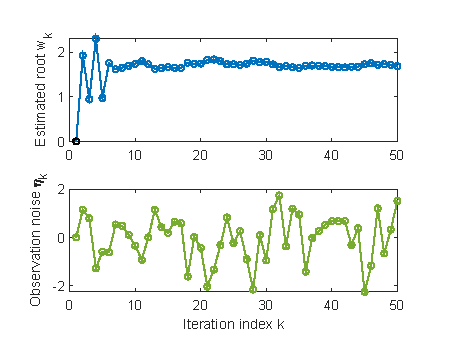
\includegraphics[width=217.1pt]{fig6_3}\par\smallskip
  \begin{minipage}{0.94\textwidth}\footnotesize
  \textbf{Figure 6.3.} An illustrative example of the RM algorithm.\par\smallskip
  \textcolor{rulegray}{\scriptsize Reproduced from S.~Zhao, \emph{Mathematical Foundations of Reinforcement Learning} (Springer, 2025).}
  \end{minipage}
\end{figure}


\subsubsection{Why does it work?}

\bk{\S6.2.1, pp.~105--106; Figure 6.4, p.~106}

Strip out the noise and take $g(w)=\tanh(w-1)$, root $w^*=1$, $w_1=3$, $a_k=1/k$.
The update is $w_{k+1}=w_k-a_kg(w_k)$, and the logic is two lines
\bkin{\S6.2.1, p.~105}:

\begin{itemize}
  \item If $w_k>w^*$ then $g(w_k)>0$, so $w_{k+1}=w_k-a_kg(w_k)<w_k$: the estimate
        moves \emph{down}, toward $w^*$.
  \item If $w_k<w^*$ then $g(w_k)<0$, so $w_{k+1}>w_k$: the estimate moves
        \emph{up}, toward $w^*$.
\end{itemize}
Provided the step $a_kg(w_k)$ is not so large that it overshoots past $w^*$, every
iteration strictly reduces the distance to the root.

\begin{figure}[htbp]
  \centering
  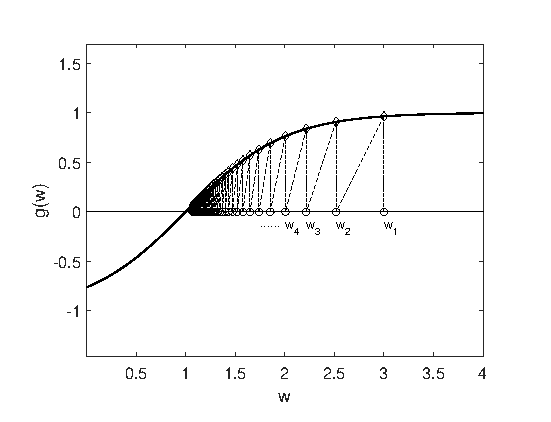
\includegraphics[width=264.7pt]{fig6_4}\par\smallskip
  \begin{minipage}{0.94\textwidth}\footnotesize
  \textbf{Figure 6.4.} An example for illustrating the convergence of the RM algorithm.\par\smallskip
  \textcolor{rulegray}{\scriptsize Reproduced from S.~Zhao, \emph{Mathematical Foundations of Reinforcement Learning} (Springer, 2025).}
  \end{minipage}
\end{figure}


\subsubsection{The convergence theorem}

\bk{Theorem 6.1, p.~106}

\begin{theorem}[Robbins--Monro, Theorem 6.1, p.~106]
In the RM algorithm (6.5), suppose
\begin{enumerate}
  \item[(a)] $0<c_1\le\nabla_w g(w)\le c_2$ for all $w$;
  \item[(b)] $\displaystyle\sum_{k=1}^\infty a_k=\infty$ and
             $\displaystyle\sum_{k=1}^\infty a_k^2<\infty$;
  \item[(c)] $\E[\eta_k\mid H_k]=0$ and $\E[\eta_k^2\mid H_k]<\infty$, where
             $H_k=\{w_k,w_{k-1},\dots\}$.
\end{enumerate}
Then $w_k$ converges almost surely to the root $w^*$ with $g(w^*)=0$.
\end{theorem}

Each condition earns its keep \bkin{\S6.2.1, pp.~106--107}.

\paragraph{(a) Monotonicity.} $\nabla_wg>0$ means $g$ is strictly increasing, which
guarantees the root exists and is \emph{unique}. If $g$ is decreasing, apply the
theorem to $-g$. In the optimisation reading $g=\nabla_wJ$, so this condition says
$J$ is convex --- the standard assumption. The upper bound $\nabla_wg\le c_2$ says
the slope cannot blow up: $\tanh(w-1)$ qualifies; $w^3-5$ does \emph{not}, which is
why the earlier example needed a sensible starting point.

\paragraph{(b) The step-size conditions.} These two conditions appear over and over
in RL, so understand them properly.

\begin{itemize}
  \item $\sum_k a_k^2<\infty$ forces $a_k\to0$. Why do we need that? Because
        $w_{k+1}-w_k=-a_k\tilde g(w_k,\eta_k)$, so if $a_k$ does not vanish the
        iterates keep jittering forever and never settle
        \bkin{\S6.2.1, p.~107}.
  \item $\sum_k a_k=\infty$ forces $a_k$ to shrink \emph{slowly}. Why? Sum the
        increments:
        \[
          w_1-w_\infty=\sum_{k=1}^\infty a_k\tilde g(w_k,\eta_k).
        \]
        If $\sum_k a_k<\infty$ then the total distance travelled is bounded by some
        finite $b$: $|w_1-w_\infty|\le b$ \bkin{equation (6.6), p.~107}. Choose a
        starting point with $|w_1-w^*|>b$ and the algorithm \emph{cannot possibly}
        reach the root --- it runs out of steam. The condition
        $\sum_k a_k=\infty$ guarantees the algorithm has infinite ``fuel'' and can
        therefore start anywhere.
\end{itemize}

\begin{worked}{$a_k=1/k$ satisfies both conditions \bkin{\S6.2.1, pp.~107--108}}
\emph{Divergence of the sum.} The harmonic numbers satisfy
$\lim_{n\to\infty}\bigl(\sum_{k=1}^n\frac1k-\ln n\bigr)=\kappa\approx0.577$, the
Euler--Mascheroni constant. Since $\ln n\to\infty$,
$\sum_{k=1}^\infty\frac1k=\infty$. \checkmark

\emph{Convergence of the squared sum.} The Basel problem gives
$\sum_{k=1}^\infty\frac1{k^2}=\frac{\pi^2}{6}<\infty$. \checkmark

Small modifications such as $a_k=1/(k+1)$, or $a_k=c_k/k$ with $c_k$ bounded, also
work.
\end{worked}

\begin{remark}[What practitioners actually do]
\bkin{\S6.2.1, p.~108} In real implementations $a_k$ is usually a small
\emph{constant}. That violates condition (b), since
$\sum a_k^2=\infty$. The algorithm still converges in a weaker sense --- it enters
and stays in a small neighbourhood of $w^*$ rather than converging to the point.
For nonstationary problems this is a feature, not a bug: a constant step size keeps
the estimate responsive to change.
\end{remark}

\paragraph{(c) Noise.} Mild. It does \emph{not} require Gaussian noise. If
$\{\eta_k\}$ is i.i.d.\ with mean zero and finite variance, then $\eta_k$ is
independent of $H_k$, so $\E[\eta_k\mid H_k]=\E[\eta_k]=0$ automatically.

\subsubsection{Mean estimation is an RM algorithm}

\bk{\S6.2.2, pp.~108--109}

\begin{worked}{casting mean estimation as root-finding}
Define $g(w)\doteq w-\E[X]$. Solving $g(w)=0$ recovers $\E[X]$. Given a sample $x$
of $X$, the observable quantity is $\tilde g=w-x$, and
\[
  \tilde g(w,\eta)= w-x = \underbrace{(w-\E[X])}_{g(w)}+\underbrace{(\E[X]-x)}_{\eta}.
\]
The RM algorithm for this $g$ reads
\[
  w_{k+1}=w_k-\alpha_k\tilde g(w_k,\eta_k)=w_k-\alpha_k(w_k-x_k),
\]
which is precisely equation (6.4). Therefore Theorem 6.1 gives: $w_k\to\E[X]$
almost surely whenever $\sum\alpha_k=\infty$, $\sum\alpha_k^2<\infty$ and
$\{x_k\}$ is i.i.d. \textbf{No assumption at all is made about the distribution of
$X$} \bkin{\S6.2.2, p.~109}.
\end{worked}

\subsection{Dvoretzky's theorem (the general convergence machinery)}

\bk{\S6.3, pp.~109--114; Theorem 6.2, p.~109; Theorem 6.3, p.~113}

This section is more mathematical and can be skimmed on a first pass; but
Theorem 6.3 is the tool used to prove Q-learning converges, so it is worth knowing
that it exists.

\begin{theorem}[Dvoretzky, Theorem 6.2, p.~109]
Consider the stochastic process
\[
  \Delta_{k+1}=(1-\alpha_k)\Delta_k+\beta_k\eta_k,
  \qquad \alpha_k\ge0,\ \beta_k\ge0 .
\]
Then $\Delta_k\to0$ almost surely provided
\begin{enumerate}
  \item[(a)] $\sum_k\alpha_k=\infty$, $\sum_k\alpha_k^2<\infty$ and
             $\sum_k\beta_k^2<\infty$ uniformly almost surely;
  \item[(b)] $\E[\eta_k\mid H_k]=0$ and $\E[\eta_k^2\mid H_k]\le C$ almost surely.
\end{enumerate}
\end{theorem}

\begin{intuition}[How to read the recursion]
$\Delta_k$ is an \emph{error}. The factor $(1-\alpha_k)$ contracts it; the term
$\beta_k\eta_k$ injects zero-mean noise. Condition (a) says: contract infinitely
often ($\sum\alpha_k=\infty$) but inject only finite total noise energy
($\sum\beta_k^2<\infty$). Signal wins, noise dies.
\end{intuition}

Unlike the RM theorem, Dvoretzky's theorem allows $\alpha_k,\beta_k$ to be
\emph{random} and to depend on the history $H_k$ \bkin{\S6.3, p.~110}. That extra
generality is exactly what is needed to prove the RM theorem itself.

\begin{proof}[Proof sketch (\S6.3.1, pp.~110--111)]
Set $h_k=\Delta_k^2$. Expanding,
\[
  h_{k+1}-h_k=-\alpha_k(2-\alpha_k)\Delta_k^2+\beta_k^2\eta_k^2+2(1-\alpha_k)\beta_k\eta_k\Delta_k .
\]
Take $\E[\cdot\mid H_k]$. Because $\Delta_k$ is $H_k$-measurable it comes out of the
expectation; the cross term vanishes since $\E[\eta_k\mid H_k]=0$; and for $k$ large
enough $\alpha_k\le1$ so $-\alpha_k(2-\alpha_k)\Delta_k^2\le0$. Hence
\[
  \E[h_{k+1}-h_k\mid H_k]\ \le\ \beta_k^2C,
  \qquad\text{so}\qquad
  \sum_k\E[h_{k+1}-h_k\mid H_k]\ \le\ C\sum_k\beta_k^2<\infty .
\]
By the quasimartingale convergence theorem, $h_k$ converges. Rearranging the same
identity shows $\sum_k\alpha_k\Delta_k^2<\infty$; combined with
$\sum_k\alpha_k=\infty$ this forces $\Delta_k\to0$.
\end{proof}

\begin{worked}{mean estimation via Dvoretzky \bkin{\S6.3.2, p.~112}}
Let $w^*=\E[X]$ and $\Delta_k=w_k-w^*$. Then
\[
  \Delta_{k+1}=\Delta_k+\alpha_k(x_k-w^*-\Delta_k)
             =(1-\alpha_k)\Delta_k+\alpha_k\underbrace{(x_k-w^*)}_{\eta_k}.
\]
Because $\{x_k\}$ is i.i.d., $\E[\eta_k\mid H_k]=\E[x_k]-w^*=0$ and
$\E[\eta_k^2\mid H_k]=\E[x_k^2]-(w^*)^2=\Var[X]<\infty$. Dvoretzky applies.
\end{worked}

\begin{worked}{proving Robbins--Monro via Dvoretzky \bkin{\S6.3.3, pp.~112--113}}
With $\Delta_k=w_k-w^*$ and $g(w^*)=0$, the mean value theorem gives
$g(w_k)-g(w^*)=\nabla_wg(w_k')(w_k-w^*)$ for some $w_k'$ between $w_k$ and $w^*$.
Then
\[
  \Delta_{k+1}=\bigl[1-\underbrace{a_k\nabla_wg(w_k')}_{\alpha_k}\bigr]\Delta_k+a_k(-\eta_k).
\]
Since $0<c_1\le\nabla_wg\le c_2$, the conditions
$\sum a_k=\infty$, $\sum a_k^2<\infty$ transfer to $\alpha_k$. Note that this
$\alpha_k$ is \emph{random} (it depends on $w_k$) --- which is exactly why we needed
Dvoretzky rather than a deterministic argument.
\end{worked}

\begin{theorem}[Multi-variable extension, Theorem 6.3, p.~113]
For a finite index set $S$ and the process
$\Delta_{k+1}(s)=(1-\alpha_k(s))\Delta_k(s)+\beta_k(s)\eta_k(s)$, we get
$\Delta_k(s)\to0$ almost surely for every $s\in S$ if, for every $s$,
\begin{enumerate}
  \item[(a)] $\sum_k\alpha_k(s)=\infty$, $\sum_k\alpha_k^2(s)<\infty$,
             $\sum_k\beta_k^2(s)<\infty$, and
             $\E[\beta_k(s)\mid H_k]\le\E[\alpha_k(s)\mid H_k]$;
  \item[(b)] $\norm{\E[\eta_k(s)\mid H_k]}_\infty\le\gamma\norm{\Delta_k}_\infty$
             with $\gamma\in(0,1)$;
  \item[(c)] $\Var[\eta_k(s)\mid H_k]\le C(1+\norm{\Delta_k(s)}_\infty)^2$.
\end{enumerate}
\end{theorem}

\begin{remark}
Read $s$ as ``state'' or ``state--action pair'' \bkin{\S6.3.4, p.~114}. Two upgrades
over Theorem 6.2: it handles many variables at once via the max-norm, and it
permits the noise to have \emph{nonzero} conditional mean, provided that mean is
bounded by $\gamma$ times the current error. That $\gamma$ is the discount rate in
disguise --- which is how the contraction property of Chapter 3 re-enters the
convergence proofs of Chapter 7. \textbf{Crucially, the conditions must hold at
every $s$}, which is the formal reason RL algorithms need every state--action pair
visited infinitely often.
\end{remark}

\subsection{Stochastic gradient descent}

\bk{\S6.4, pp.~114--123}

\subsubsection{Three algorithms, one problem}

\bk{\S6.4, pp.~114--115; equations (6.10)--(6.13)}

The problem \bkin{equation (6.10), p.~114}:
\[
  \min_w\ J(w)=\E[f(w,X)].
\]

\textbf{Gradient descent (GD)} \bkin{equation (6.11), p.~114}:
\[
  w_{k+1}=w_k-\alpha_k\nabla_wJ(w_k)=w_k-\alpha_k\,\E[\nabla_wf(w_k,X)].
\]
Unusable when the distribution of $X$ is unknown --- and it usually is.

\textbf{Batch approximation} \bkin{equation (6.12), p.~115}:
\[
  w_{k+1}=w_k-\frac{\alpha_k}{n}\sum_{i=1}^n\nabla_wf(w_k,x_i).
\]
Better, but it needs all $n$ samples at every single iteration.

\textbf{Stochastic gradient descent (SGD)} \bkin{equation (6.13), p.~115}:
\[
  \boxed{\;w_{k+1}=w_k-\alpha_k\nabla_wf(w_k,x_k).\;}
\]
One sample per update.

\begin{intuition}[Why replacing the gradient by one noisy sample is legitimate]
\bkin{\S6.4, p.~115} Decompose
\[
  \nabla_wf(w_k,x_k)=\E[\nabla_wf(w_k,X)]
    +\underbrace{\bigl(\nabla_wf(w_k,x_k)-\E[\nabla_wf(w_k,X)]\bigr)}_{\eta_k},
\]
so SGD is exactly GD plus a perturbation:
$w_{k+1}=w_k-\alpha_k\E[\nabla_wf(w_k,X)]-\alpha_k\eta_k$. Because $\{x_k\}$ is
i.i.d., $\E[\eta_k]=0$. A zero-mean perturbation with a decaying step size averages
itself away.
\end{intuition}

\subsubsection{Mean estimation is an SGD algorithm}

\bk{\S6.4.1, p.~116; equation (6.14)}

\begin{worked}{closing the circle}
Pose mean estimation as an optimisation \bkin{equation (6.14), p.~116}:
\[
  \min_w\ J(w)=\E\Bigl[\tfrac12\norm{w-X}^2\Bigr],
  \qquad f(w,X)=\tfrac12\norm{w-X}^2,\qquad \nabla_wf(w,X)=w-X .
\]
Setting $\nabla_wJ(w)=\E[w-X]=0$ gives $w^*=\E[X]$. \checkmark

\emph{GD:} $w_{k+1}=w_k-\alpha_k\E[w_k-X]$ --- unusable, since $\E[X]$ is the
very thing we are trying to find.

\emph{SGD:} $w_{k+1}=w_k-\alpha_k(w_k-x_k)$ --- which is equation (6.4) again.

So we have the chain
\[
  \text{mean estimation} \subset \text{SGD} \subset \text{RM algorithm},
\]
each a special case of the next \bkin{\S6.5, p.~123}. That is the architecture of
the whole chapter.
\end{worked}

\subsubsection{The convergence pattern of SGD}

\bk{\S6.4.2, pp.~116--118; equation (6.15); Figure 6.5, p.~118}

Does the randomness make SGD slow? The answer is a specific and useful one.

Define the relative error between the stochastic and true gradients:
\[
  \delta_k\doteq\frac{\abs{\nabla_wf(w_k,x_k)-\E[\nabla_wf(w_k,X)]}}
                     {\abs{\E[\nabla_wf(w_k,X)]}} .
\]
Since $\E[\nabla_wf(w^*,X)]=0$, the denominator can be rewritten and expanded by
the mean value theorem \bkin{equation (6.15), p.~117}, giving, when $f$ is strictly
convex with $\nabla^2_wf\ge c>0$,
\[
  \delta_k\ \le\
  \frac{\overbrace{\abs{\nabla_wf(w_k,x_k)-\E[\nabla_wf(w_k,X)]}}^{\text{noise in the gradient}}}
       {c\underbrace{\abs{w_k-w^*}}_{\text{distance to the optimum}}} .
\]

\begin{intuition}[The headline result]
\textbf{The relative error is inversely proportional to how far you are from the
optimum.} Far away, the true gradient is large and the sampling noise is
proportionally negligible, so SGD behaves like plain gradient descent and converges
fast. Close to the optimum, the true gradient is nearly zero and the noise
dominates, so the iterates rattle around in a neighbourhood
\bkin{\S6.4.2, p.~117}.

For mean estimation this is exact:
$\delta_k=\frac{\abs{\E[X]-x_k}}{\abs{w_k-w^*}}$, so the typical size of $\delta_k$
is proportional to the standard deviation of $X$ and inversely proportional to the
distance from the answer \bkin{\S6.4.2, p.~117}.
\end{intuition}

The book illustrates this with $X$ uniform on a square of side $20$ centred at the
origin, $\E[X]=0$, and $100$ i.i.d.\ samples: the estimate rockets in from a distant
initial guess and then wobbles near the origin \bkin{Figure 6.5, p.~118}.

\subsubsection{The deterministic formulation}

\bk{\S6.4.3, pp.~118--119; equation (6.16)}

You will often see SGD written with no random variables anywhere:
\[
  \min_w\ J(w)=\frac1n\sum_{i=1}^n f(w,x_i),
  \qquad\text{updated as}\qquad
  w_{k+1}=w_k-\alpha_k\nabla_wf(w_k,x_k),
  \tag{6.16}
\]
where $x_k$ is ``the item fetched at step $k$'', not ``the $k$th item of the list''.
Is this really SGD? And should we cycle through the list in order or sample at
random?

\begin{remark}[The answer, \bkin{\S6.4.3, p.~119}]
Introduce a random variable $X$ uniform on $\{x_1,\dots,x_n\}$, so $p(X=x_i)=1/n$.
Then
\[
  \frac1n\sum_{i=1}^n f(w,x_i)=\E[f(w,X)]
\]
\emph{exactly} --- not approximately. So (6.16) \textbf{is} SGD, and it converges
\emph{provided $x_k$ is sampled uniformly and independently} from the set. Sampling
with replacement means the same item may be drawn twice, which is fine. Marching
through the list in a fixed order is \emph{not} covered by the theory.
\end{remark}

\subsubsection{BGD, MBGD and SGD}

\bk{\S6.4.4, pp.~119--121}

\[
\begin{aligned}
  \text{BGD:}\quad & w_{k+1}=w_k-\alpha_k\frac1n\sum_{i=1}^n\nabla_wf(w_k,x_i)\\
  \text{MBGD:}\quad& w_{k+1}=w_k-\alpha_k\frac1m\sum_{j\in\mathcal I_k}\nabla_wf(w_k,x_j),
                     \qquad |\mathcal I_k|=m\\
  \text{SGD:}\quad & w_{k+1}=w_k-\alpha_k\nabla_wf(w_k,x_k)
\end{aligned}
\]

\begin{warning}
Setting $m=1$ turns MBGD into SGD. But setting $m=n$ does \emph{not} turn MBGD into
BGD \bkin{\S6.4.4, p.~120}. MBGD draws $n$ samples \emph{randomly, with
replacement}, so it may draw some items twice and miss others; BGD uses each of the
$n$ items exactly once. A subtle point, and a favourite exam question.
\end{warning}

\begin{worked}{all three on mean estimation \bkin{\S6.4.4, pp.~120--121}}
Minimise $J(w)=\frac{1}{2n}\sum_i\norm{w-x_i}^2$, optimum $w^*=\bar x$. The three
updates become
\[
  \text{BGD: } w_{k+1}=w_k-\alpha_k(w_k-\bar x),\quad
  \text{MBGD: } w_{k+1}=w_k-\alpha_k(w_k-\bar x_k^{(m)}),\quad
  \text{SGD: } w_{k+1}=w_k-\alpha_k(w_k-x_k),
\]
with $\bar x_k^{(m)}=\frac1m\sum_{j\in\mathcal I_k}x_j$. With $\alpha_k=1/k$ these
unroll to
\[
  \text{BGD: } w_{k+1}=\frac1k\sum_{j=1}^k\bar x=\bar x,\qquad
  \text{MBGD: } w_{k+1}=\frac1k\sum_{j=1}^k\bar x_j^{(m)},\qquad
  \text{SGD: } w_{k+1}=\frac1k\sum_{j=1}^k x_j .
\]
BGD lands on the exact answer at every step (it had all the information from the
start). MBGD converges faster than SGD because each of its increments is already an
average and hence less noisy. In the book's simulation, $m=50$ converges fastest,
$m=5$ next, and $m=1$ (SGD) slowest --- though SGD is still quick while it is far
from the answer, exactly as \S6.4.2 predicts \bkin{Figure 6.5, p.~118}.
\end{worked}

\begin{figure}[htbp]
  \centering
  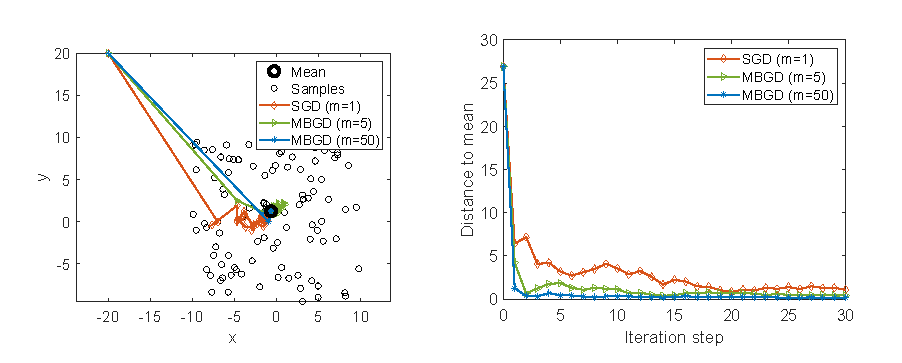
\includegraphics[width=433.1pt]{fig6_5}\par\smallskip
  \begin{minipage}{0.94\textwidth}\footnotesize
  \textbf{Figure 6.5.} An example for demonstrating stochastic and mini-batch gradient descent algorithms. The distribution of X $\in$R2 is uniform in the square area centered at the origin with a side length as 20. The mean is E[X] = 0. The mean estimation is based on 100 i.i.d. samples.\par\smallskip
  \textcolor{rulegray}{\scriptsize Reproduced from S.~Zhao, \emph{Mathematical Foundations of Reinforcement Learning} (Springer, 2025).}
  \end{minipage}
\end{figure}


\subsubsection{Convergence of SGD}

\bk{\S6.4.5, pp.~121--123; Theorem 6.4, p.~121; Box 6.1, p.~122}

\begin{theorem}[Convergence of SGD, Theorem 6.4, p.~121]
For the SGD algorithm (6.13), $w_k$ converges almost surely to the root of
$\nabla_w\E[f(w,X)]=0$ if
\begin{enumerate}
  \item[(a)] $0<c_1\le\nabla_w^2f(w,X)\le c_2$ (strong convexity with bounded
             curvature; in the vector case $\nabla^2_wf$ is the Hessian);
  \item[(b)] $\sum_k a_k=\infty$ and $\sum_k a_k^2<\infty$;
  \item[(c)] $\{x_k\}$ are i.i.d.
\end{enumerate}
\end{theorem}

\begin{proof}[Proof (Box 6.1, pp.~122--123): SGD is a special RM algorithm]
Set $g(w)=\nabla_wJ(w)=\E[\nabla_wf(w,X)]$; SGD looks for the root of $g(w)=0$. The
measurable quantity is
\[
  \tilde g(w,\eta)=\nabla_wf(w,x)=\underbrace{\E[\nabla_wf(w,X)]}_{g(w)}
    +\underbrace{\bigl(\nabla_wf(w,x)-\E[\nabla_wf(w,X)]\bigr)}_{\eta},
\]
so the RM algorithm $w_{k+1}=w_k-a_k\tilde g(w_k,\eta_k)$ \emph{is} SGD. Now check
Theorem 6.1's conditions: (a)
$\nabla_wg(w)=\E[\nabla^2_wf(w,X)]\in[c_1,c_2]$; (b) identical; (c) since $x_k$ is
independent of $H_k=\{w_k,w_{k-1},\dots\}$,
$\E[\eta_k\mid H_k]=\E_{x_k}[\nabla_wf(w_k,x_k)]-\E[\nabla_wf(w_k,X)]=0$, and
$\E[\eta_k^2\mid H_k]<\infty$ whenever the gradient is bounded.
\end{proof}

\subsection{Chapter 6 summary and self-check}

\bk{\S6.5, p.~123}

\begin{center}
\small
\begin{tabular}{@{}lp{0.60\textwidth}@{}}
\toprule
Result & Why you need it later \\
\midrule
Incremental mean update (6.4) & The template for the TD update in Chapter 7. \\
RM algorithm (6.5) & TD learning \emph{is} an RM algorithm applied to the Bellman equation \bkin{\S7.1.2, p.~128}. \\
Step-size conditions $\sum a_k=\infty,\ \sum a_k^2<\infty$ & Reappear verbatim in Theorems 7.1 and 7.2. \\
Dvoretzky, Theorem 6.3 & The machinery behind the convergence of Sarsa and Q-learning. \\
SGD & The optimiser for every function-approximation method in Chapters 8--10. \\
\bottomrule
\end{tabular}
\end{center}

\begin{enumerate}
  \item Derive $w_{k+1}=w_k-\frac1k(w_k-x_k)$ from the definition of the running
        average, then verify $w_3=\frac12(x_1+x_2)$.
  \item Explain, using the ``fuel'' argument, why $\sum_k a_k=\infty$ is necessary,
        and construct a step-size sequence that fails it.
  \item Show $a_k=1/\sqrt k$ satisfies $\sum a_k=\infty$ but violates
        $\sum a_k^2<\infty$. What behaviour would you predict?
  \item Why is SGD fast far from the optimum and noisy near it? Give the inequality.
  \item Explain why MBGD with $m=n$ is not BGD.
  \item Show that mean estimation is simultaneously an instance of MC estimation
        (Chapter 5), of SGD, and of the RM algorithm.
\end{enumerate}

\newpage
% ============================================================
\section{Temporal-Difference Methods}
% ============================================================

\begin{roadmap}{Chapter 7 of the textbook}
\textbf{Textbook:} Chapter 7, pp.~125--150. Sections: \S7.1 TD learning of state
values (p.~126; algorithm p.~126, properties p.~128, convergence p.~130),
\S7.2 Sarsa (p.~133; algorithm p.~133, optimal policy learning p.~134),
\S7.3 $n$-step Sarsa (p.~138), \S7.4 Q-learning (p.~140; algorithm p.~140,
off-policy vs on-policy p.~141, implementation p.~144, examples p.~144),
\S7.5 a unified viewpoint (p.~145), \S7.6 summary (p.~148), \S7.7 Q\&A (p.~149).
Algorithms 7.1 (p.~135), 7.2 (p.~143), 7.3 (p.~143). Table 7.2 (p.~148).\\[0.3em]
\textbf{Videos:}
\vid{L7 P1 --- Motivating example}{https://www.youtube.com/watch?v=u1X-7XX3dtI};
\vid{L7 P2 --- TD: introduction}{https://www.youtube.com/watch?v=XiCUsc7CCE0};
\vid{L7 P3 --- TD: convergence}{https://www.youtube.com/watch?v=faWg8M91-Oo};
\vid{L7 P4 --- Sarsa}{https://www.youtube.com/watch?v=jYwQufkBUPo};
\vid{L7 P5 --- Expected \& $n$-step Sarsa}{https://www.youtube.com/watch?v=0kKzQbWZOlk};
\vid{L7 P6 --- Q-learning: introduction}{https://www.youtube.com/watch?v=4BvYR2hm730};
\vid{L7 P7 --- Q-learning: pseudocode}{https://www.youtube.com/watch?v=I0YhlOIFF4s};
\vid{L7 P8 --- Unified viewpoint}{https://www.youtube.com/watch?v=3t74lvk1GBM}.\\[0.3em]
\textbf{One sentence:} every algorithm in this chapter is a stochastic approximation
algorithm (Chapter 6) applied to a Bellman equation (Chapter 2) or to the Bellman
optimality equation (Chapter 3).
\end{roadmap}

\begin{figure}[htbp]
  \centering
  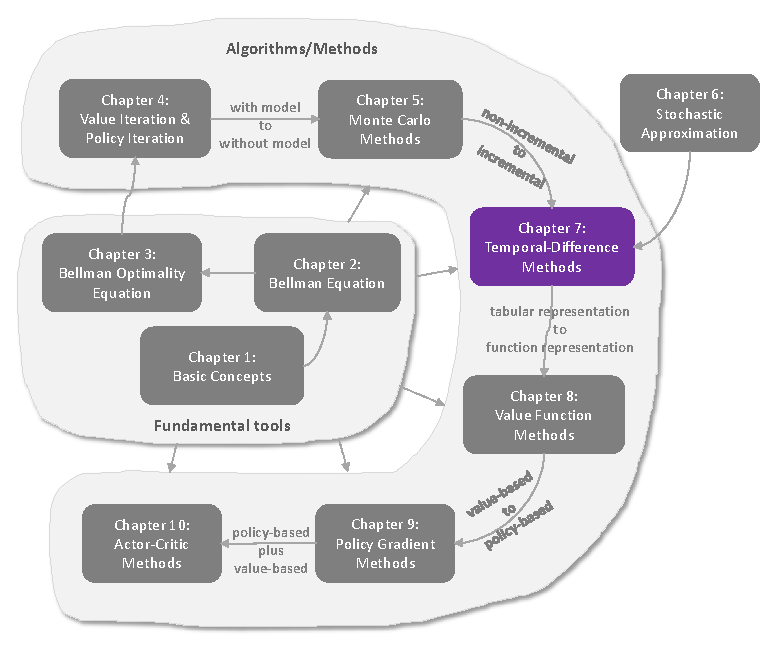
\includegraphics[width=371.3pt]{fig7_1}\par\smallskip
  \begin{minipage}{0.94\textwidth}\footnotesize
  \textbf{Figure 7.1.} Where we are in this book.\par\smallskip
  \textcolor{rulegray}{\scriptsize Reproduced from S.~Zhao, \emph{Mathematical Foundations of Reinforcement Learning} (Springer, 2025).}
  \end{minipage}
\end{figure}


\subsection{TD learning of state values}

\bk{\S7.1.1, pp.~126--128; equations (7.1)--(7.5)}

Given a policy $\pi$ and a stream of experience
$(s_0,r_1,s_1,\dots,s_t,r_{t+1},s_{t+1},\dots)$ generated by $\pi$, we want
$v_\pi(s)$ for all $s$.

\begin{definition}[TD learning of state values, equations (7.1)--(7.2), p.~126]
\[
  \boxed{\;
  v_{t+1}(s_t)=v_t(s_t)-\alpha_t(s_t)\Bigl[v_t(s_t)-\bigl(r_{t+1}+\gamma v_t(s_{t+1})\bigr)\Bigr],
  \;}
\]
\[
  v_{t+1}(s)=v_t(s)\quad\text{for all }s\neq s_t .
\]
\end{definition}

\begin{warning}
The second line is not decorative. \textbf{At each time step only the state you
actually visited is updated}; every other state keeps its old estimate. The book
notes that this line is often omitted for brevity but that the algorithm is
mathematically incomplete without it \bkin{\S7.1.1, p.~126}.
\end{warning}

\subsubsection{Where does this update come from?}

\bk{Box 7.1, pp.~127--128}

Start from the definition of the state value and use bootstrapping:
\[
  v_\pi(s)=\E\bigl[R_{t+1}+\gamma G_{t+1}\mid S_t=s\bigr]
  \tag{7.3}
\]
and, because
$\E[G_{t+1}\mid S_t=s]=\sum_a\pi(a\mid s)\sum_{s'}p(s'\mid s,a)v_\pi(s')=\E[v_\pi(S_{t+1})\mid S_t=s]$,
\[
  \boxed{\;v_\pi(s)=\E\bigl[R_{t+1}+\gamma v_\pi(S_{t+1})\mid S_t=s\bigr]\;}
  \tag{7.4}
\]
which the book calls the \textbf{Bellman expectation equation}
\bkin{\S7.1.1, p.~127}. It is exactly the Bellman equation of Chapter 2, rewritten
as an expectation.

\begin{worked}{deriving the TD update from Robbins--Monro \bkin{Box 7.1, pp.~127--128}}
Define
\[
  g(v_\pi(s_t))\doteq v_\pi(s_t)-\E\bigl[R_{t+1}+\gamma v_\pi(S_{t+1})\mid S_t=s_t\bigr],
\]
so that (7.4) is the statement $g(v_\pi(s_t))=0$: a \textbf{root-finding problem}.
We cannot evaluate $g$ (it contains an unknown expectation), but from the sample
$(s_t,r_{t+1},s_{t+1})$ we can form the noisy observation
\[
  \tilde g(v_\pi(s_t))=v_\pi(s_t)-\bigl(r_{t+1}+\gamma v_\pi(s_{t+1})\bigr)
  = \underbrace{g(v_\pi(s_t))}_{\text{signal}}
   +\underbrace{\E[R_{t+1}+\gamma v_\pi(S_{t+1})\mid s_t]-\bigl(r_{t+1}+\gamma v_\pi(s_{t+1})\bigr)}_{\eta,\ \text{zero mean}} .
\]
Feed this into the RM algorithm $w_{k+1}=w_k-a_k\tilde g$ (equation (6.5)) and out
comes
\[
  v_{t+1}(s_t)=v_t(s_t)-\alpha_t(s_t)\bigl[v_t(s_t)-(r_{t+1}+\gamma v_\pi(s_{t+1}))\bigr].
  \tag{7.5}
\]
One gap remains: (7.5) contains the \emph{true} $v_\pi(s_{t+1})$, which we do not
know. Replace it by the current estimate $v_t(s_{t+1})$ and you get (7.1). Whether
that substitution preserves convergence is exactly the content of Theorem 7.1
\bkin{Box 7.1, p.~128}.
\end{worked}

\subsubsection{TD target and TD error}

\bk{\S7.1.2, pp.~128--129; equation (7.6)}

Rewrite the update with names attached \bkin{equation (7.6), p.~128}:
\[
  \underbrace{v_{t+1}(s_t)}_{\text{new estimate}}
  =\underbrace{v_t(s_t)}_{\text{current estimate}}
   -\alpha_t(s_t)\Bigl[\overbrace{v_t(s_t)-\underbrace{\bigl(r_{t+1}+\gamma v_t(s_{t+1})\bigr)}_{\text{TD target }\bar v_t}}^{\text{TD error }\delta_t}\Bigr].
\]

\paragraph{Why ``target''?} Subtract $\bar v_t$ from both sides
\bkin{\S7.1.2, p.~128}:
\[
  v_{t+1}(s_t)-\bar v_t=\bigl[1-\alpha_t(s_t)\bigr]\bigl(v_t(s_t)-\bar v_t\bigr)
  \quad\Longrightarrow\quad
  \abs{v_{t+1}(s_t)-\bar v_t}<\abs{v_t(s_t)-\bar v_t}
\]
whenever $0<\alpha_t(s_t)<1$. The update provably moves the estimate \emph{toward}
$\bar v_t$. Hence the name.

\paragraph{Why ``temporal difference''?} Because
$\delta_t=v_t(s_t)-(r_{t+1}+\gamma v_t(s_{t+1}))$ compares quantities at two
consecutive times $t$ and $t+1$.

\paragraph{What does the error measure?} If the estimates were correct,
$v_t=v_\pi$, then
\[
  \E[\delta_t\mid S_t=s_t]
  =v_\pi(s_t)-\E[R_{t+1}+\gamma v_\pi(S_{t+1})\mid s_t]=0
\]
by (7.4). \textbf{So the TD error is zero in expectation exactly when the estimate
is right} \bkin{\S7.1.2, p.~129}. A nonzero TD error is therefore evidence that the
current value function is wrong, and its size says by how much.

\begin{intuition}[Innovation]
\bkin{\S7.1.2, p.~129} The book flags the deeper reading: $\delta_t$ is the
\textbf{innovation} --- the genuinely new information contained in the sample
$(s_t,r_{t+1},s_{t+1})$ that was not already in $v_t$. This is the same notion as
the innovation in Kalman filtering. TD learning is: form a prediction, observe,
compute the surprise, and correct the prediction in proportion to the surprise.
\end{intuition}

\subsubsection{TD versus Monte Carlo}

\bk{Table 7.1, p.~130}

\begin{center}
\small
\begin{tabular}{@{}p{0.46\textwidth}p{0.46\textwidth}@{}}
\toprule
\textbf{TD learning} & \textbf{MC learning}\\
\midrule
\textbf{Incremental.} Updates immediately after each single transition.
& \textbf{Non-incremental.} Must wait for a complete episode before it can compute a return. \\[0.4em]
\textbf{Continuing tasks.} Works with or without terminal states.
& \textbf{Episodic tasks only.} Needs episodes that terminate in finite time. \\[0.4em]
\textbf{Bootstraps.} The update of $v(s_t)$ uses the current estimate $v(s_{t+1})$, so an initial guess is required.
& \textbf{Does not bootstrap.} Estimates values directly from returns; no initial guess needed. \\[0.4em]
\textbf{Low variance.} Sarsa needs samples of only three random variables: $R_{t+1},S_{t+1},A_{t+1}$.
& \textbf{High variance.} $q_\pi(s_t,a_t)$ requires a sample of $R_{t+1}+\gamma R_{t+2}+\gamma^2R_{t+3}+\cdots$. With episode length $L$ and $|\Aspace|$ actions per state there are $|\Aspace|^L$ possible episodes. \\
\bottomrule
\end{tabular}
\end{center}

\begin{intuition}[The bias--variance trade-off in one line]
MC is unbiased but noisy: it uses the real return, but the real return depends on
every random choice for the rest of the episode. TD is biased but calm: it replaces
the far future by a current guess $v_t(s_{t+1})$ --- wrong at first, but it collapses
the randomness of the entire remaining episode into a single number. Chapter 7's
$n$-step Sarsa is the dial between the two.
\end{intuition}

\subsubsection{Convergence}

\bk{\S7.1.3, pp.~130--132; Theorem 7.1, p.~130; proof in Box 7.2, pp.~131--132}

\begin{theorem}[Convergence of TD learning, Theorem 7.1, p.~130]
Given a policy $\pi$, the TD algorithm (7.1) satisfies $v_t(s)\to v_\pi(s)$ almost
surely for every $s\in\Sspace$, provided
$\sum_t\alpha_t(s)=\infty$ and $\sum_t\alpha_t^2(s)<\infty$ \textbf{for every}
$s\in\Sspace$.
\end{theorem}

\begin{proof}[Proof sketch (Box 7.2, pp.~131--132)]
Let $\Delta_t(s)=v_t(s)-v_\pi(s)$. Subtracting $v_\pi(s)$ from the update gives, for
$s=s_t$,
\[
  \Delta_{t+1}(s)=(1-\alpha_t(s))\Delta_t(s)
    +\alpha_t(s)\underbrace{\bigl(r_{t+1}+\gamma v_t(s_{t+1})-v_\pi(s)\bigr)}_{\eta_t(s)},
\]
and for $s\neq s_t$ the same expression holds with $\alpha_t(s)=\eta_t(s)=0$. This
is precisely the process of Theorem 6.3. Condition (a) is the hypothesis.
Condition (b) is the interesting one: for $s=s_t$, using
$v_\pi(s_t)=\E[r_{t+1}+\gamma v_\pi(s_{t+1})\mid s_t]$,
\[
  \abs{\E[\eta_t(s)]}=\gamma\Bigl|\sum_{s'}p(s'\mid s_t)[v_t(s')-v_\pi(s')]\Bigr|
  \le\gamma\max_{s'}\abs{v_t(s')-v_\pi(s')}=\gamma\norm{\Delta_t}_\infty,
\]
which is exactly condition (b) of Theorem 6.3 \bkin{equation (7.11), p.~132}.
Condition (c) follows since $r_{t+1}$ is bounded.
\end{proof}

\begin{remark}[Two practical readings of the step-size condition]
\bkin{\S7.1.3, pp.~130--131}
\begin{itemize}
  \item $\alpha_t(s)>0$ only when $s$ is the state visited at time $t$; otherwise it
        is $0$. So $\sum_t\alpha_t(s)=\infty$ demands that \emph{every state be
        visited infinitely often}. This is exploration, entering through the back
        door of a convergence proof.
  \item In practice $\alpha$ is a small constant, which violates
        $\sum\alpha_t^2<\infty$. The algorithm then converges only in a weaker
        sense. The book gives the real reason a constant is used
        \bkin{\S7.7 Q\&A, p.~149}: during optimal-policy learning the policy being
        evaluated \emph{keeps changing}, so the target is nonstationary; a decaying
        step size would eventually be too small to track it.
\end{itemize}
\end{remark}

\subsection{Sarsa}

\bk{\S7.2, pp.~133--137; equation (7.12), p.~133; Algorithm 7.1, p.~135}

Estimating $v_\pi$ is not enough --- policy improvement needs $q_\pi$. Take the TD
update and replace state values with action values.

\begin{definition}[Sarsa, equation (7.12), p.~133]
Given samples $(s_0,a_0,r_1,s_1,a_1,\dots)$ generated by $\pi$,
\[
  \boxed{\;
  q_{t+1}(s_t,a_t)=q_t(s_t,a_t)-\alpha_t(s_t,a_t)
    \Bigl[q_t(s_t,a_t)-\bigl(r_{t+1}+\gamma q_t(s_{t+1},a_{t+1})\bigr)\Bigr],\;}
\]
with $q_{t+1}(s,a)=q_t(s,a)$ for all $(s,a)\neq(s_t,a_t)$.
\end{definition}

\begin{remark}[The name]
Each update consumes the quintuple $(s_t,a_t,r_{t+1},s_{t+1},a_{t+1})$ ---
\textbf{s}tate, \textbf{a}ction, \textbf{r}eward, \textbf{s}tate, \textbf{a}ction
\bkin{\S7.2.1, p.~133}.
\end{remark}

\textbf{What is it solving?} The Bellman equation in action-value form
\bkin{equation (7.13), p.~133; proof in Box 7.3, p.~134}:
\[
  q_\pi(s,a)=\E\bigl[R+\gamma q_\pi(S',A')\mid s,a\bigr]\qquad\text{for all }(s,a).
\]

\begin{theorem}[Convergence of Sarsa, Theorem 7.2, p.~134]
$q_t(s,a)\to q_\pi(s,a)$ almost surely for all $(s,a)$ provided
$\sum_t\alpha_t(s,a)=\infty$ and $\sum_t\alpha_t^2(s,a)<\infty$ for every
$(s,a)$ --- which requires every \emph{state--action pair} to be visited infinitely
often.
\end{theorem}

\subsubsection{Finding optimal policies with Sarsa}

\bk{\S7.2.2, pp.~134--136; Algorithm 7.1, p.~135}

\begin{algobox}{Optimal policy learning by Sarsa (Algorithm 7.1, p.~135)}
\textbf{Initialise:} $\alpha_t(s,a)=\alpha>0$; $\varepsilon\in(0,1)$;
$q_0(s,a)$; an $\varepsilon$-greedy $\pi_0$ derived from $q_0$.\\
\textbf{Goal:} learn a policy that leads the agent from $s_0$ to the target state.\\
For each episode:
\begin{itemize}\itemsep0pt
  \item Generate $a_0$ at $s_0$ following $\pi_0(s_0)$.
  \item While $s_t$ is not the target state:
    \begin{itemize}\itemsep0pt
      \item Interact with the environment to obtain $r_{t+1},s_{t+1}$; generate
            $a_{t+1}$ following $\pi_t(s_{t+1})$.
      \item \textbf{Value update:}
            $q_{t+1}(s_t,a_t)=q_t(s_t,a_t)-\alpha_t(s_t,a_t)\bigl[q_t(s_t,a_t)-(r_{t+1}+\gamma q_t(s_{t+1},a_{t+1}))\bigr]$.
      \item \textbf{Policy update ($\varepsilon$-greedy at $s_t$ only):}
            $\pi_{t+1}(a\mid s_t)=1-\frac{\varepsilon}{|\Aspace(s_t)|}(|\Aspace(s_t)|-1)$
            if $a=\argmax_a q_{t+1}(s_t,a)$, else $\frac{\varepsilon}{|\Aspace(s_t)|}$.
      \item $s_t\leftarrow s_{t+1}$, $a_t\leftarrow a_{t+1}$.
    \end{itemize}
\end{itemize}
\end{algobox}

\begin{remark}
Notice how aggressive this is: \emph{one} sample updates \emph{one} $q$-value, and
the policy at that state is immediately revised and immediately used to generate the
next sample. There is no attempt to evaluate the policy accurately before improving
it. This is generalised policy iteration taken to its limit
\bkin{\S7.2.2, p.~135}.
\end{remark}

\begin{worked}{Sarsa finding a path \bkin{Figure 7.2, p.~136}}
\textbf{Setup.} $5\times5$ grid. Every episode starts at the top-left cell and ends
at the target. Rewards: $r_{\text{target}}=0$,
$r_{\text{forbidden}}=r_{\text{boundary}}=-10$, $r_{\text{other}}=-1$. Constant
$\alpha=0.1$, $\varepsilon=0.1$, $q_0(s,a)=0$, and $\pi_0$ uniform ($0.2$ each).

Note the task has changed: we want an optimal \emph{path from one starting state},
not optimal policies for all states \bkin{\S7.2.2, p.~135}. That is much cheaper ---
only states near the path need exploring --- but the answer may be locally rather
than globally optimal.

\textbf{Results over 500 episodes.}
\begin{itemize}
  \item \emph{Total reward per episode} rises steadily from about $-400$ toward $0$:
        early policies keep hitting walls and forbidden cells.
  \item \emph{Episode length} falls from over $200$ steps toward a short path.
  \item \emph{Spikes.} Around episode $460$ the length jumps and the reward
        collapses. Why? The policy is $\varepsilon$-greedy, so with probability
        $\varepsilon$ it takes a bad action, and a single bad action early in an
        episode can cost a lot. \textbf{The remedy is a decaying $\varepsilon$}
        \bkin{\S7.2.2, p.~136}.
  \item The final policy reaches the target reliably, but the policies at states far
        from the path are \emph{not} optimal, because they were never explored.
\end{itemize}
\end{worked}

\begin{figure}[htbp]
  \centering
  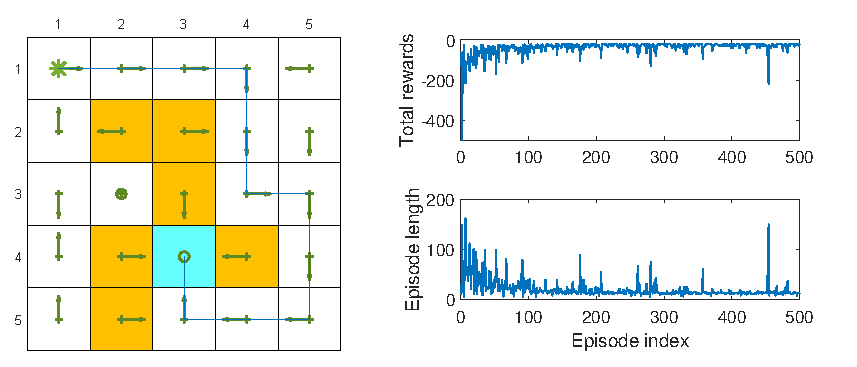
\includegraphics[width=411.4pt]{fig7_2}\par\smallskip
  \begin{minipage}{0.94\textwidth}\footnotesize
  \textbf{Figure 7.2.} An example for demonstrating Sarsa. All the episodes start from the top-left state and terminate when reaching the target state (the blue cell). The goal is to find an optimal path from the starting state to the target state. The reward settings are rtarget = 0, rforbidden = rboundary = $-$10, and rother = $-$1. The learning rate is $\alpha$ = 0.1 and the value of $\varepsilon$ is 0.1. The left figure shows the final policy obtained by the algorithm. The right figures show the total reward and length of every episode.\par\smallskip
  \textcolor{rulegray}{\scriptsize Reproduced from S.~Zhao, \emph{Mathematical Foundations of Reinforcement Learning} (Springer, 2025).}
  \end{minipage}
\end{figure}


\subsubsection{Expected Sarsa}

\bk{Box 7.4, p.~137; equation (7.15)}

\begin{definition}[Expected Sarsa]
\[
  q_{t+1}(s_t,a_t)=q_t(s_t,a_t)-\alpha_t(s_t,a_t)
    \Bigl[q_t(s_t,a_t)-\bigl(r_{t+1}+\gamma\,\E[q_t(s_{t+1},A)]\bigr)\Bigr],
\]
where
$\E[q_t(s_{t+1},A)]=\sum_a\pi_t(a\mid s_{t+1})q_t(s_{t+1},a)\doteq v_t(s_{t+1})$.
\end{definition}

The only change is the TD target: $r_{t+1}+\gamma\E[q_t(s_{t+1},A)]$ instead of
$r_{t+1}+\gamma q_t(s_{t+1},a_{t+1})$.

\begin{intuition}
Why bother computing an expectation? \textbf{Variance reduction.} Sarsa's target
depends on the random draw $a_{t+1}$; Expected Sarsa averages that draw out
analytically. The random variables shrink from
$\{s_t,a_t,r_{t+1},s_{t+1},a_{t+1}\}$ to $\{s_t,a_t,r_{t+1},s_{t+1}\}$
\bkin{Box 7.4, p.~137}. You pay a little computation and buy a lot of stability ---
the same trade you make when you use a conditional expectation instead of a single
draw anywhere in statistics.
\end{intuition}

Substituting $\E[q_\pi(S_{t+1},A_{t+1})\mid S_{t+1}]=v_\pi(S_{t+1})$ into (7.15)
shows Expected Sarsa solves
$q_\pi(s,a)=\E[R_{t+1}+\gamma v_\pi(S_{t+1})\mid s,a]$ --- the Bellman equation once
again \bkin{Box 7.4, p.~137}.

\subsection{$n$-step Sarsa}

\bk{\S7.3, pp.~138--139; equation (7.17)}

The return admits a whole family of decompositions \bkin{\S7.3, pp.~138--139}:
\[
\begin{aligned}
  G_t^{(1)}&=R_{t+1}+\gamma q_\pi(S_{t+1},A_{t+1}) &&\longleftarrow\text{Sarsa}\\
  G_t^{(2)}&=R_{t+1}+\gamma R_{t+2}+\gamma^2q_\pi(S_{t+2},A_{t+2})\\
  &\ \ \vdots\\
  G_t^{(n)}&=R_{t+1}+\gamma R_{t+2}+\cdots+\gamma^nq_\pi(S_{t+n},A_{t+n})
    &&\longleftarrow n\text{-step Sarsa}\\
  &\ \ \vdots\\
  G_t^{(\infty)}&=R_{t+1}+\gamma R_{t+2}+\gamma^2R_{t+3}+\cdots
    &&\longleftarrow\text{Monte Carlo}
\end{aligned}
\]

\begin{warning}
$G_t=G_t^{(1)}=G_t^{(2)}=\cdots=G_t^{(\infty)}$ --- these are all \emph{the same
random variable}. The superscripts label different ways of writing it, not different
quantities \bkin{\S7.3, p.~138}. What differs is which pieces we replace by
estimates.
\end{warning}

\begin{definition}[$n$-step Sarsa, equation (7.17), p.~139]
\[
  q_{t+1}(s_t,a_t)=q_t(s_t,a_t)-\alpha_t(s_t,a_t)
   \Bigl[q_t(s_t,a_t)-\bigl(r_{t+1}+\gamma r_{t+2}+\cdots+\gamma^nq_t(s_{t+n},a_{t+n})\bigr)\Bigr].
\]
\end{definition}

\begin{remark}[Implementation detail]
At time $t$ you do not yet have $(r_{t+n},s_{t+n},a_{t+n})$, so the update for
$(s_t,a_t)$ must wait until time $t+n$ \bkin{\S7.3, p.~139}:
\[
  q_{t+n}(s_t,a_t)=q_{t+n-1}(s_t,a_t)-\alpha_{t+n-1}(s_t,a_t)
   \bigl[q_{t+n-1}(s_t,a_t)-(r_{t+1}+\cdots+\gamma^nq_{t+n-1}(s_{t+n},a_{t+n}))\bigr].
\]
\end{remark}

\begin{intuition}[The dial]
$n=1$ gives Sarsa; $n=\infty$ with $\alpha_t=1$ gives MC learning. In between:
\begin{itemize}
  \item \textbf{large $n$} $\Rightarrow$ close to MC: \emph{small bias, large
        variance} (more real rewards, more randomness);
  \item \textbf{small $n$} $\Rightarrow$ close to Sarsa: \emph{large bias, small
        variance} (more reliance on a possibly-wrong bootstrap).
\end{itemize}
\bkin{\S7.3, p.~139}
\end{intuition}

\subsection{Q-learning}

\bk{\S7.4, pp.~140--145; equation (7.18), p.~140; Box 7.5, pp.~140--141}

\begin{definition}[Q-learning, equation (7.18), p.~140]
\[
  \boxed{\;
  q_{t+1}(s_t,a_t)=q_t(s_t,a_t)-\alpha_t(s_t,a_t)
    \Bigl[q_t(s_t,a_t)-\bigl(r_{t+1}+\gamma\max_{a\in\Aspace(s_{t+1})}q_t(s_{t+1},a)\bigr)\Bigr],\;}
\]
with all other $q$-values unchanged.
\end{definition}

Two differences from Sarsa, both consequential \bkin{\S7.4.1, p.~140}:

\begin{center}
\small
\begin{tabular}{@{}lll@{}}
\toprule
 & Sarsa & Q-learning \\
\midrule
TD target & $r_{t+1}+\gamma q_t(s_{t+1},a_{t+1})$ & $r_{t+1}+\gamma\max_a q_t(s_{t+1},a)$ \\
Samples needed & $(s_t,a_t,r_{t+1},s_{t+1},a_{t+1})$ & $(s_t,a_t,r_{t+1},s_{t+1})$ \\
Equation solved & Bellman equation of $\pi$ & \textbf{Bellman optimality equation} \\
\bottomrule
\end{tabular}
\end{center}

\textbf{What it solves} \bkin{equation (7.19), p.~140}:
\[
  q(s,a)=\E\Bigl[R_{t+1}+\gamma\max_a q(S_{t+1},a)\ \Big|\ S_t=s,A_t=a\Bigr].
\]

\begin{proof}[This is the BOE (Box 7.5, pp.~140--141)]
Write the expectation out:
$q(s,a)=\sum_r p(r\mid s,a)r+\gamma\sum_{s'}p(s'\mid s,a)\max_{a}q(s',a)$. Take
$\max_{a\in\Aspace(s)}$ of both sides and set $v(s)\doteq\max_a q(s,a)$:
\[
  v(s)=\max_{a\in\Aspace(s)}\Bigl[\sum_r p(r\mid s,a)r+\gamma\sum_{s'}p(s'\mid s,a)v(s')\Bigr],
\]
which is the Bellman optimality equation of Chapter 3 \bkin{equation (3.1), p.~38}.
\end{proof}

\begin{intuition}[Why the $\max$ changes everything]
The $\max$ says: ``when I evaluate the consequence of $(s_t,a_t)$, assume I will
behave optimally from $s_{t+1}$ onward --- regardless of what I \emph{actually} do
next.'' That single word decouples what the agent learns about from what the agent
does, which is exactly the definition of off-policy learning.
\end{intuition}

\subsubsection{On-policy versus off-policy}

\bk{\S7.4.2, pp.~141--143}

\begin{definition}
Every RL task involves two policies. The \textbf{behaviour policy} generates the
experience samples. The \textbf{target policy} is the one being improved toward
optimality. If they coincide, the learning is \textbf{on-policy}; if they may
differ, it is \textbf{off-policy}.
\end{definition}

\paragraph{Sarsa is on-policy.} Its samples are generated as
\[
  s_t\xrightarrow{\ \pi_b\ }a_t\xrightarrow{\ \text{model}\ }r_{t+1},s_{t+1}
     \xrightarrow{\ \pi_b\ }a_{t+1}.
\]
The target $r_{t+1}+\gamma q_t(s_{t+1},a_{t+1})$ contains $a_{t+1}$, which was drawn
from $\pi_b$. So the policy being evaluated is the policy generating the data
\bkin{\S7.4.2, p.~142}.

\paragraph{Q-learning is off-policy.} Its samples are generated as
\[
  s_t\xrightarrow{\ \pi_b\ }a_t\xrightarrow{\ \text{model}\ }r_{t+1},s_{t+1},
\]
and the target $r_{t+1}+\gamma\max_a q_t(s_{t+1},a)$ contains \emph{no} action drawn
from $\pi_b$ --- the $\max$ is computed over the table. The generation of
$(r_{t+1},s_{t+1})$ is governed by the environment, not by $\pi_b$. Hence $\pi_b$ may
be anything \bkin{\S7.4.2, p.~142}.

\paragraph{MC learning is on-policy}, for the same reason as Sarsa.

\begin{intuition}[Why off-policy is valuable]
\bkin{\S7.4.2, p.~141} You can learn an optimal policy from data generated by
someone else --- a human operator, an old policy, a logged dataset. In particular
you can use a \emph{strongly exploratory} behaviour policy (say uniform random) to
guarantee coverage, while the target policy converges to something purely greedy.
Sarsa cannot do this: its exploration is capped by $\varepsilon$, which must stay
small to keep the learned policy good, so it is squeezed from both sides.
\end{intuition}

\begin{warning}[On/off-policy is not online/offline]
\bkin{\S7.4.2, p.~143} \emph{Online} means updating while interacting with the
environment; \emph{offline} means updating from pre-collected data. An on-policy
algorithm can be run online but cannot consume other policies' logged data. An
off-policy algorithm can be run either way.
\end{warning}

\subsubsection{Two implementations}

\bk{\S7.4.3, p.~144; Algorithms 7.2 and 7.3, p.~143}

\begin{algobox}{Q-learning, on-policy version (Algorithm 7.2, p.~143)}
\textbf{Initialise:} $\alpha>0$, $\varepsilon\in(0,1)$, $q_0(s,a)$, and an
$\varepsilon$-greedy $\pi_0$.\\
For each episode, while $s_t$ is not the target state:
\begin{itemize}\itemsep0pt
  \item Generate $a_t$ following $\pi_t(s_t)$; obtain $r_{t+1},s_{t+1}$ from the
        environment.
  \item $q_{t+1}(s_t,a_t)=q_t(s_t,a_t)-\alpha_t(s_t,a_t)\bigl[q_t(s_t,a_t)-(r_{t+1}+\gamma\max_a q_t(s_{t+1},a))\bigr]$.
  \item Update $\pi$ at $s_t$ to be \textbf{$\varepsilon$-greedy} w.r.t.\ $q_{t+1}$.
\end{itemize}
\end{algobox}

\begin{algobox}{Q-learning, off-policy version (Algorithm 7.3, p.~143)}
\textbf{Initialise:} $q_0(s,a)$; a behaviour policy $\pi_b(a\mid s)$; $\alpha>0$.\\
For each episode $\{s_0,a_0,r_1,s_1,a_1,r_2,\dots\}$ \textbf{generated by $\pi_b$}:
\begin{itemize}\itemsep0pt
  \item For each step $t$:
    \begin{itemize}\itemsep0pt
      \item $q_{t+1}(s_t,a_t)=q_t(s_t,a_t)-\alpha_t(s_t,a_t)\bigl[q_t(s_t,a_t)-(r_{t+1}+\gamma\max_a q_t(s_{t+1},a))\bigr]$.
      \item Update the target policy at $s_t$ to be \textbf{greedy}:
            $\pi_{T,t+1}(a\mid s_t)=1$ if $a=\argmax_a q_{t+1}(s_t,a)$, else $0$.
    \end{itemize}
\end{itemize}
\end{algobox}

\begin{remark}
Why greedy in Algorithm 7.3 but $\varepsilon$-greedy in Algorithm 7.2? Because in
the off-policy version the target policy is never used to collect data, so it has no
obligation to explore \bkin{\S7.7 Q\&A, p.~150}.
\end{remark}

\subsubsection{What the experiments show}

\bk{\S7.4.4, pp.~144--145; Figures 7.3--7.5, pp.~144--147}

\begin{worked}{on-policy Q-learning finding a path \bkin{Figure 7.3, p.~144}}
Same setup as the Sarsa run ($r_{\text{target}}=0$,
$r_{\text{forbidden}}=r_{\text{boundary}}=-10$, $r_{\text{other}}=-1$,
$\alpha=0.1$, $\varepsilon=0.1$). Over 500 episodes the episode length falls and the
total reward rises, and an optimal path is found --- qualitatively the same picture
as Sarsa.
\end{worked}

\begin{figure}[htbp]
  \centering
  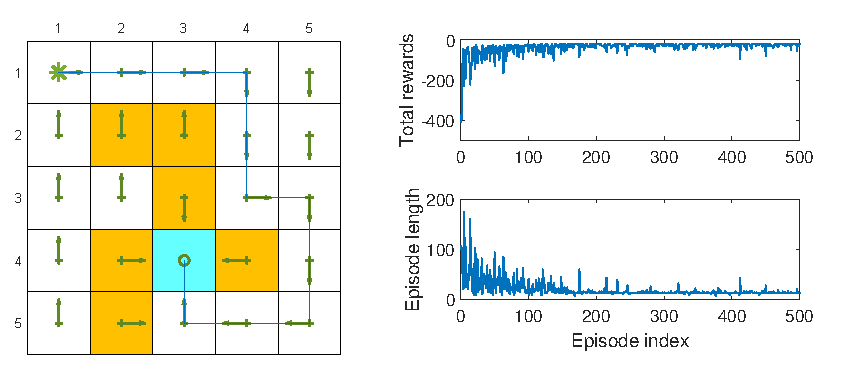
\includegraphics[width=411.4pt]{fig7_3}\par\smallskip
  \begin{minipage}{0.94\textwidth}\footnotesize
  \textbf{Figure 7.3.} An example for demonstrating Q-learning. All the episodes start from the top-left state and terminate after reaching the target state. The aim is to find an optimal path from the starting state to the target state. The reward settings are rtarget = 0, rforbidden = rboundary = $-$10, and rother = $-$1. The learning rate is $\alpha$ = 0.1 and the value of $\varepsilon$ is 0.1. The left figure shows the final policy obtained by the algorithm. The right figure shows the total reward and length of every episode.\par\smallskip
  \textcolor{rulegray}{\scriptsize Reproduced from S.~Zhao, \emph{Mathematical Foundations of Reinforcement Learning} (Springer, 2025).}
  \end{minipage}
\end{figure}


\begin{worked}{off-policy Q-learning learning \emph{every} state's policy \bkin{Figure 7.4, pp.~146}}
Setup: $r_{\text{boundary}}=r_{\text{forbidden}}=-1$, $r_{\text{target}}=1$,
$\gamma=0.9$, $\alpha=0.1$.

\textbf{Ground truth} (from model-based policy iteration): optimal values
\[
\begin{array}{ccccc}
5.8&5.6&6.2&6.5&5.8\\
6.5&7.2&8.0&7.2&6.5\\
7.2&8.0&10.0&8.0&7.2\\
8.0&10.0&10.0&10.0&8.0\\
7.2&9.0&10.0&9.0&8.1
\end{array}
\]

\textbf{Data:} a behaviour policy that is uniform ($0.2$ on every action), used to
generate \emph{one} episode of $100{,}000$ steps. Because the behaviour policy
explores well, that single episode visits every state--action pair many times.

\textbf{Result:} the learned target policy is optimal, and the RMS error of the
estimated state values converges to zero. Note it is not the \emph{same} arrow
pattern as the ground-truth figure --- and that is fine, because optimal policies are
not unique (\S3.4) \bkin{\S7.4.4, p.~145}.

\textbf{Sensitivity to the initial guess:} Q-learning bootstraps, so $q_0$ matters.
A good $q_0$ converges in roughly $10{,}000$ steps; a poor one needs more --- but
still converges quickly \bkin{Figure 7.4(g)--(h)}.

\textbf{Sensitivity to the behaviour policy \bkin{Figure 7.5, p.~147}:} with
$\varepsilon$-greedy behaviour policies at $\varepsilon=1$ (uniform), then $0.5$,
then $0.1$, the learning speed degrades \emph{sharply}. Weak exploration means many
state--action pairs are barely visited, so their values are never learned.
\textbf{Off-policy learning does not free you from needing exploration; it frees you
from needing the \emph{target} policy to provide it.}
\end{worked}

\begin{figure}[htbp]
  \centering
  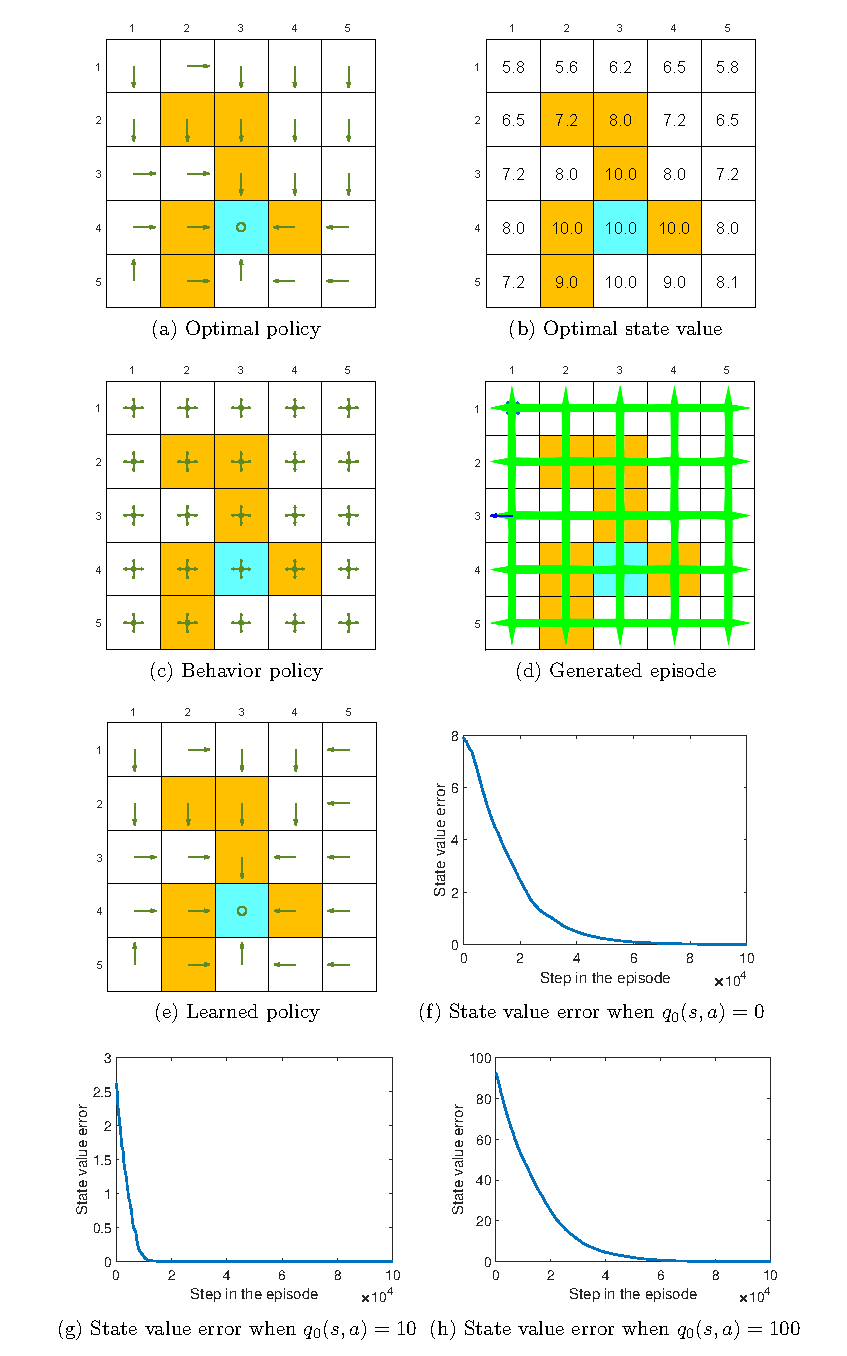
\includegraphics[width=251.9pt]{fig7_4}\par\smallskip
  \begin{minipage}{0.94\textwidth}\footnotesize
  \textbf{Figure 7.4.} Examples for demonstrating off-policy learning via Q-learning. The optimal policy and optimal state values are shown in (a) and (b), respectively. The behavior policy and the generated episode are shown in (c) and (d), respectively. The estimated policy and the estimation error evolution are shown in (e) and (f), respectively. The cases with different initial values are shown in (g) and (h).\par\smallskip
  \textcolor{rulegray}{\scriptsize Reproduced from S.~Zhao, \emph{Mathematical Foundations of Reinforcement Learning} (Springer, 2025).}
  \end{minipage}
\end{figure}


\subsection{A unified viewpoint}

\bk{\S7.5, pp.~145--148; Table 7.2, p.~148}

Every action-value TD algorithm has the same skeleton
\bkin{equation (7.20), p.~145}:
\[
  \boxed{\;q_{t+1}(s_t,a_t)=q_t(s_t,a_t)-\alpha_t(s_t,a_t)\bigl[q_t(s_t,a_t)-\bar q_t\bigr]\;}
\]
and differs only in the TD target $\bar q_t$.

\begin{center}
\small
\begin{tabular}{@{}lll@{}}
\toprule
Algorithm & TD target $\bar q_t$ & Equation being solved \\
\midrule
Sarsa & $r_{t+1}+\gamma q_t(s_{t+1},a_{t+1})$
      & BE: $q_\pi(s,a)=\E[R_{t+1}+\gamma q_\pi(S_{t+1},A_{t+1})\mid s,a]$\\
$n$-step Sarsa & $r_{t+1}+\gamma r_{t+2}+\cdots+\gamma^n q_t(s_{t+n},a_{t+n})$
      & BE: $q_\pi(s,a)=\E[R_{t+1}+\cdots+\gamma^n q_\pi(S_{t+n},A_{t+n})\mid s,a]$\\
Q-learning & $r_{t+1}+\gamma\max_a q_t(s_{t+1},a)$
      & \textbf{BOE:} $q(s,a)=\E[R_{t+1}+\gamma\max_a q(S_{t+1},a)\mid s,a]$\\
Monte Carlo & $r_{t+1}+\gamma r_{t+2}+\gamma^2r_{t+3}+\cdots$
      & BE: $q_\pi(s,a)=\E[R_{t+1}+\gamma R_{t+2}+\cdots\mid s,a]$\\
\bottomrule
\end{tabular}
\end{center}

MC learning is the special case $\alpha_t(s_t,a_t)=1$, which collapses the update to
$q_{t+1}(s_t,a_t)=\bar q_t$ \bkin{\S7.5, p.~148}.

\begin{remark}[The one-line summary of the chapter]
\textbf{Every algorithm here solves the Bellman equation of a given policy ---
except Q-learning, which solves the Bellman optimality equation.} That single
distinction explains why Q-learning is off-policy and the rest are on-policy
\bkin{\S7.6, p.~148}.
\end{remark}

\begin{figure}[htbp]
  \centering
  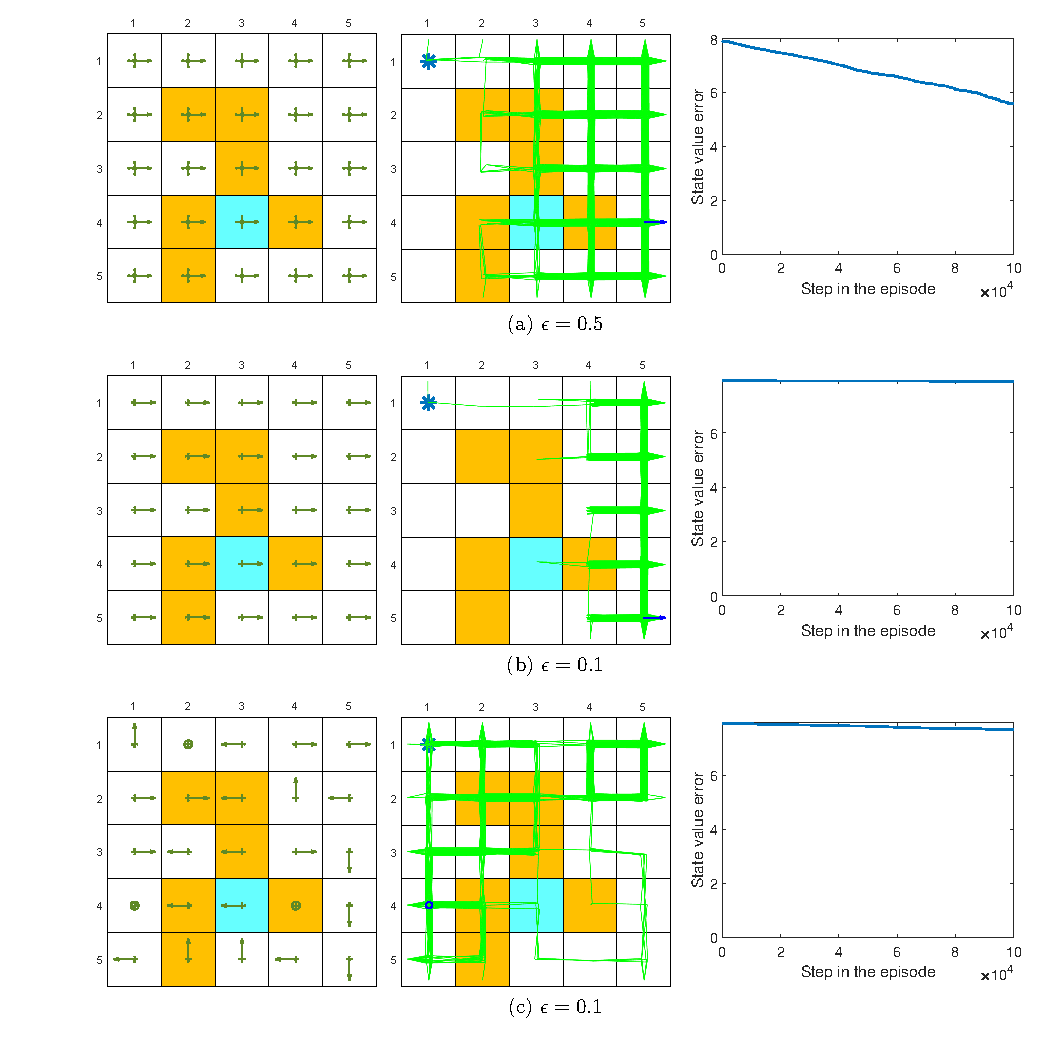
\includegraphics[width=413.6pt]{fig7_5}\par\smallskip
  \begin{minipage}{0.94\textwidth}\footnotesize
  \textbf{Figure 7.5.} The performance of Q-learning drops when the behavior policy is not exploratory. The figures in the left column show the behavior policies. The figures in the middle column show the generated episodes following the corresponding behavior policies. The episode in each example has 100,000 steps. The figures in the right column show the evolution of the root-mean-square error of the estimated state values.\par\smallskip
  \textcolor{rulegray}{\scriptsize Reproduced from S.~Zhao, \emph{Mathematical Foundations of Reinforcement Learning} (Springer, 2025).}
  \end{minipage}
\end{figure}


\subsection{Chapter 7 self-check}

\begin{enumerate}
  \item Write the TD update and identify the TD target and TD error. Prove that the
        update moves $v_t(s_t)$ strictly closer to the target.
  \item Show that $\E[\delta_t\mid S_t=s_t]=0$ when $v_t=v_\pi$, and explain why this
        makes $\delta_t$ a sensible learning signal.
  \item Which of TD and MC has higher variance, and why? Which is biased?
  \item Sarsa's target uses $a_{t+1}$; Q-learning's uses $\max_a$. Explain in two
        sentences why this makes one on-policy and the other off-policy.
  \item In Figure 7.2, why does the episode length spike near episode 460, and what
        would you change to prevent it?
  \item Theorem 7.1 requires $\sum_t\alpha_t(s)=\infty$ for every $s$. Translate this
        condition into a statement about exploration.
  \item Fill in the unified table from memory: four algorithms, four TD targets, four
        equations.
\end{enumerate}

\newpage
% ============================================================
\section{Value Function Methods}
% ============================================================

\begin{roadmap}{Chapter 8 of the textbook}
\textbf{Textbook:} Chapter 8, pp.~151--190. Sections: \S8.1 from table to function
(p.~152), \S8.2 TD learning of state values with function approximation (p.~155;
objective function p.~156, optimisation algorithms p.~161, choosing approximators
p.~162, examples p.~164, theory p.~167), \S8.3 TD learning of action values
(p.~179; Sarsa p.~179, Q-learning p.~180), \S8.4 deep Q-learning (p.~181; algorithm
p.~182, examples p.~184), \S8.5 summary (p.~186), \S8.6 Q\&A (p.~187).
Algorithms 8.1 (p.~163), 8.2 (p.~180), 8.3 (p.~183). Boxes 8.1--8.6, pp.~157--176.\\[0.3em]
\textbf{Videos:}
\vid{L8 P1 --- Curve fitting}{https://www.youtube.com/watch?v=uJXcI8fcdWc};
\vid{L8 P2 --- Objective function}{https://www.youtube.com/watch?v=Z3HI1TfpJP0};
\vid{L8 P3 --- Optimisation algorithm}{https://www.youtube.com/watch?v=piBDwrKt0uU};
\vid{L8 P4 --- Examples and analysis}{https://www.youtube.com/watch?v=VFyBNEZxMMs};
\vid{L8 P5 --- Sarsa and Q-learning}{https://www.youtube.com/watch?v=C-HtY4-W_zw};
\vid{L8 P6 --- DQN basic idea}{https://www.youtube.com/watch?v=lZCcbZbqVSQ};
\vid{L8 P7 --- DQN experience replay}{https://www.youtube.com/watch?v=rynEdAdebi0};
\vid{L8 P8 --- DQN implementation}{https://www.youtube.com/watch?v=vQHuCHjd6hA}.\\[0.3em]
\textbf{The one change:} values stop being a lookup table and become a
\emph{parametric function}. Everything else in this chapter follows from that.
\end{roadmap}

\begin{figure}[htbp]
  \centering
  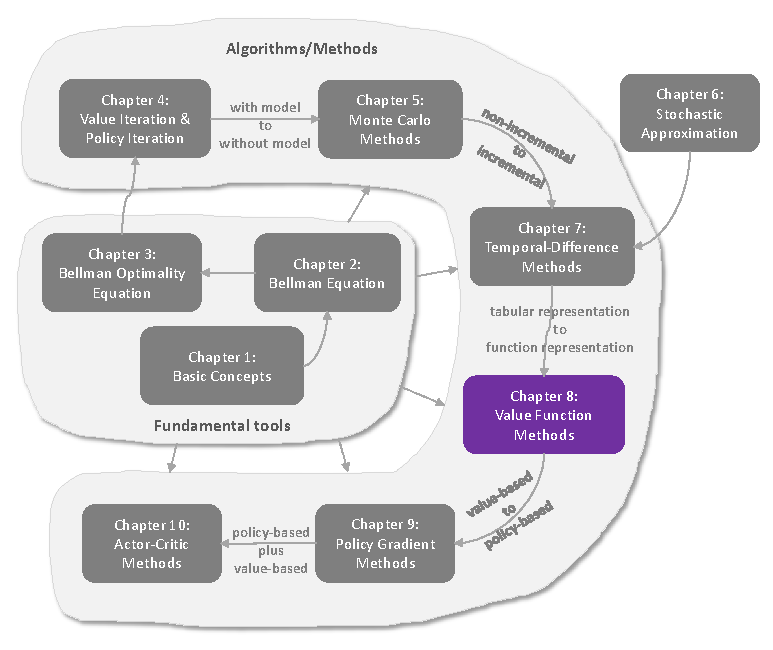
\includegraphics[width=371.3pt]{fig8_1}\par\smallskip
  \begin{minipage}{0.94\textwidth}\footnotesize
  \textbf{Figure 8.1.} Where we are in this book.\par\smallskip
  \textcolor{rulegray}{\scriptsize Reproduced from S.~Zhao, \emph{Mathematical Foundations of Reinforcement Learning} (Springer, 2025).}
  \end{minipage}
\end{figure}


\subsection{From table to function}

\bk{\S8.1, pp.~152--155; Figures 8.2--8.4, pp.~152--154; equations (8.1)--(8.2)}

Until now, $n$ states meant $n$ stored numbers $\hat v(s_1),\dots,\hat v(s_n)$.
Plot those $n$ points $(s_i,\hat v(s_i))$ and fit a curve through them. The simplest
curve is a line \bkin{equation (8.1), p.~152}:
\[
  \hat v(s,w)=as+b=\underbrace{[s,\ 1]}_{\phi^{\!\top}(s)}\underbrace{\begin{bmatrix}a\\b\end{bmatrix}}_{w}
  =\phi^{\!\top}(s)w .
\]
Here $\phi(s)$ is the \textbf{feature vector} of $s$ and $w$ the parameter vector.
A quadratic works too \bkin{equation (8.2), p.~154}:
$\hat v(s,w)=as^2+bs+c=[s^2,s,1]\,[a,b,c]^{\!\top}$.

\begin{intuition}[An economist already knows this]
This is a regression. $\hat v(s,w)=\phi^{\!\top}(s)w$ is a linear model with
regressors $\phi(s)$ and coefficients $w$. If you knew the true values
$\{v_\pi(s_i)\}$ you would just run OLS: minimise
$J_1=\sum_i(\phi^{\!\top}(s_i)w-v_\pi(s_i))^2=\norm{\Phi w-v_\pi}^2$ with solution
$w^*=(\Phi^{\!\top}\Phi)^{-1}\Phi^{\!\top}v_\pi$ \bkin{\S8.1, p.~155}. The entire
difficulty of this chapter is that the ``dependent variable'' $v_\pi$ is unobserved
and must be bootstrapped.
\end{intuition}

Two things change once values live in a function.

\paragraph{Retrieving a value \bkin{\S8.1, pp.~152--153}.} With a table you read the
entry. With a function you must \emph{compute} $\phi(s)$ and then
$\phi^{\!\top}(s)w$ (or run a forward pass through a network). The pay-off is
storage: you keep $m$ numbers instead of $n$, with $m\ll n$. The cost is
\textbf{accuracy}: a straight line cannot pass through arbitrary points. Compressing
high-dimensional data into a low-dimensional vector must lose information. Hence
``approximation''.

\begin{figure}[htbp]
  \centering
  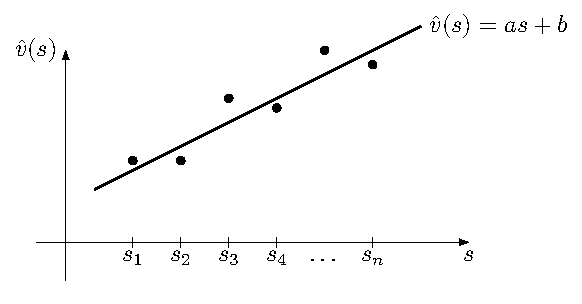
\includegraphics[width=279.5pt]{fig8_2}\par\smallskip
  \begin{minipage}{0.94\textwidth}\footnotesize
  \textbf{Figure 8.2.} An illustration of the function approximation method. The x-axis and y-axis correspond to s and \^\{\}v(s), respectively.\par\smallskip
  \textcolor{rulegray}{\scriptsize Reproduced from S.~Zhao, \emph{Mathematical Foundations of Reinforcement Learning} (Springer, 2025).}
  \end{minipage}
\end{figure}


\begin{figure}[htbp]
  \centering
  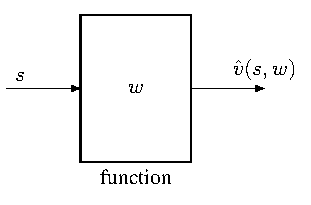
\includegraphics[width=149.2pt]{fig8_3}\par\smallskip
  \begin{minipage}{0.94\textwidth}\footnotesize
  \textbf{Figure 8.3.} An illustration of the process for retrieving the value of s when using the function approxi- mation method.\par\smallskip
  \textcolor{rulegray}{\scriptsize Reproduced from S.~Zhao, \emph{Mathematical Foundations of Reinforcement Learning} (Springer, 2025).}
  \end{minipage}
\end{figure}


\paragraph{Updating a value \bkin{\S8.1, pp.~153--154; Figure 8.4}.} With a table
you rewrite one entry and nothing else moves. With a function you change $w$, and
changing $w$ moves the value of \emph{every} state at once.

\begin{intuition}[Generalisation: the real prize]
Suppose you observe a sample only at $s_3$. The tabular method updates $\hat v(s_3)$
and leaves $\hat v(s_1),\hat v(s_2)$ untouched. The function method updates $w$,
which shifts the whole curve, so $\hat v(s_1)$ and $\hat v(s_2)$ also improve --- even
though those states were never visited \bkin{Figure 8.4, p.~154}. \textbf{One
experience teaches you about states you have never seen.} That is what makes
large-scale RL possible, and it is why the DQN example below needs $1{,}000$ steps
where tabular Q-learning needed $100{,}000$.
\end{intuition}

\begin{figure}[htbp]
  \centering
  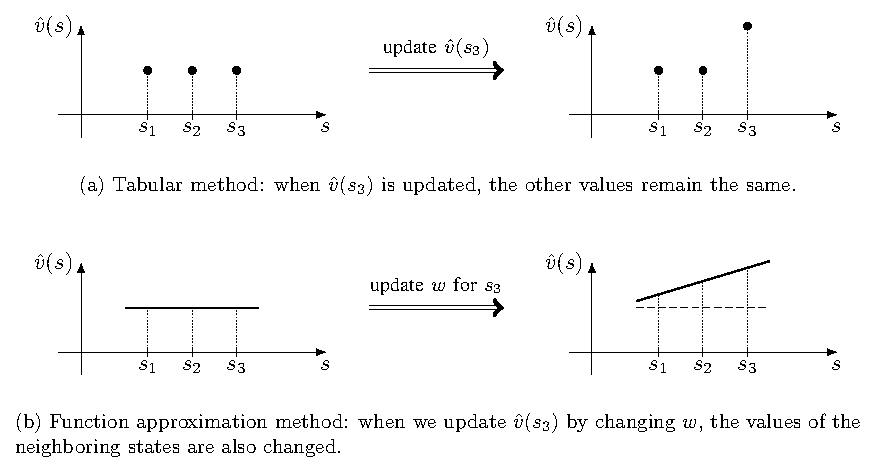
\includegraphics[width=420.1pt]{fig8_4}\par\smallskip
  \begin{minipage}{0.94\textwidth}\footnotesize
  \textbf{Figure 8.4.} An illustration of how to update the value of a state.\par\smallskip
  \textcolor{rulegray}{\scriptsize Reproduced from S.~Zhao, \emph{Mathematical Foundations of Reinforcement Learning} (Springer, 2025).}
  \end{minipage}
\end{figure}


\begin{remark}[Linear versus nonlinear]
$\hat v(s,w)=\phi^{\!\top}(s)w$ is linear \emph{in $w$}, though possibly nonlinear in
$s$. This is \textbf{linear function approximation}. Its difficulty is choosing
$\phi$, which requires knowing something about the task in advance --- and you
usually do not. The alternative is a neural network as a black-box nonlinear
approximator \bkin{\S8.1, pp.~154--155}.
\end{remark}

\subsection{The objective function}

\bk{\S8.2.1, pp.~156--161; equations (8.3)--(8.5); Box 8.1, pp.~157--161}

\begin{definition}[Value-error objective, equation (8.3), p.~156]
\[
  J(w)=\E\bigl[(v_\pi(S)-\hat v(S,w))^2\bigr].
\]
\end{definition}

An expectation with respect to $S$ --- but distributed how? Two answers
\bkin{\S8.2.1, p.~156}:

\begin{itemize}
  \item \textbf{Uniform:} $J(w)=\frac1n\sum_s(v_\pi(s)-\hat v(s,w))^2$
        \bkin{equation (8.4)}. Simple, but it treats a state the agent almost never
        reaches as equal in importance to one it occupies constantly.
  \item \textbf{Stationary distribution:}
        $J(w)=\sum_s d_\pi(s)(v_\pi(s)-\hat v(s,w))^2$ \bkin{equation (8.5), p.~157}.
        Weight each state by how often the agent actually ends up there in the long
        run. This is the book's choice.
\end{itemize}

\subsubsection{The stationary distribution}

\bk{Box 8.1, pp.~157--161; equations (8.6)--(8.10)}

Let $P_\pi$ be the transition matrix under $\pi$. Then $[P_\pi^k]_{ij}$ is the
probability of going from $s_i$ to $s_j$ in exactly $k$ steps. If $d_0$ is the
initial state distribution, then $d_k^{\!\top}=d_0^{\!\top}P_\pi^k$
\bkin{equation (8.7), p.~158}. Under suitable conditions
$\lim_{k\to\infty}P_\pi^k=\mathbf 1_nd_\pi^{\!\top}$, and therefore
\[
  \lim_{k\to\infty}d_k^{\!\top}=d_0^{\!\top}\mathbf 1_nd_\pi^{\!\top}=d_\pi^{\!\top},
\]
\emph{independently of $d_0$} \bkin{equation (8.9), p.~158}. Taking limits in
$d_k^{\!\top}=d_{k-1}^{\!\top}P_\pi$ gives the defining equation
\[
  \boxed{\;d_\pi^{\!\top}=d_\pi^{\!\top}P_\pi\;}
  \tag{8.10}
\]
so $d_\pi$ is the left eigenvector of $P_\pi$ for eigenvalue $1$, normalised to sum
to one \bkin{p.~159}.

\begin{remark}[When does it exist and is it unique?]
\bkin{Box 8.1, p.~159} A Markov process is \textbf{irreducible} if every state is
reachable from every other in finitely many steps, and \textbf{regular} if there is
a single $k$ with $P_\pi^k>0$ elementwise. Regular implies irreducible. Regular
processes have a unique stationary distribution with $d_\pi(s)>0$ for all $s$.
\textbf{Which policies give regular chains? Exploratory ones} --- an
$\varepsilon$-greedy policy assigns positive probability to every action at every
state, so states communicate whenever the environment allows \bkin{p.~160}. Once
again, exploration turns out to be a hypothesis of a theorem.
\end{remark}

\begin{worked}{computing $d_\pi$ two ways \bkin{Figure 8.5, p.~160}}
A $2\times2$ grid under an $\varepsilon$-greedy policy with $\varepsilon=0.5$, with
$s_1,s_2,s_3,s_4$ the top-left, top-right, bottom-left, bottom-right cells.

\textbf{Theory.} The chain is irreducible (all states communicate) and regular
(each state can transition to itself). Here
\[
  P_\pi^{\!\top}=\begin{pmatrix}
  0.3&0.1&0.1&0\\
  0.1&0.3&0&0.1\\
  0.6&0&0.3&0.1\\
  0&0.6&0.6&0.8
  \end{pmatrix}.
\]
Its eigenvalues are $\{-0.0449,\ 0.3,\ 0.4449,\ 1\}$. The unit eigenvector for
eigenvalue $1$ is $[0.0463,0.1455,0.1785,0.9720]^{\!\top}$; rescaling to sum to one,
\[
  d_\pi=[0.0345,\ 0.1084,\ 0.1330,\ 0.7241]^{\!\top}.
\]
So the agent spends about $72\%$ of its time in the bottom-right cell.

\textbf{Simulation.} Start at $s_1$, run $1{,}000$ steps under the policy, and record
the fraction of time spent in each state. The empirical frequencies converge to the
theoretical values after a few hundred steps \bkin{Figure 8.5, p.~160}.
\end{worked}

\begin{remark}
We will never need to \emph{compute} $d_\pi$ --- doing so would require $P_\pi$,
i.e.\ the model. It appears only in the analysis \bkin{\S8.2.1, p.~157}. This is a
recurring pattern: the model shows up in the theory and vanishes from the algorithm.
\end{remark}

\begin{figure}[htbp]
  \centering
  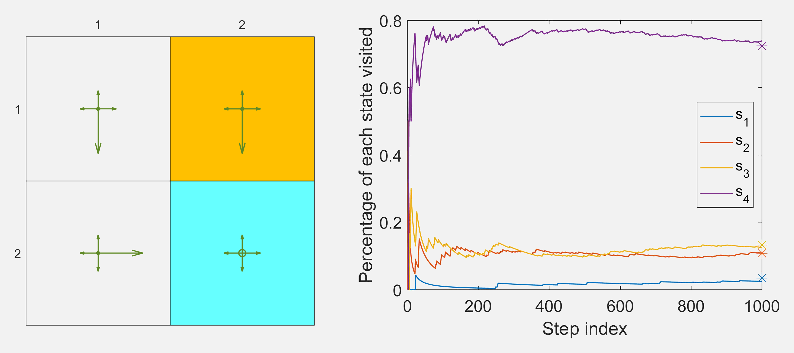
\includegraphics[width=381.3pt]{fig8_5}\par\smallskip
  \begin{minipage}{0.94\textwidth}\footnotesize
  \textbf{Figure 8.5.} Long-term behavior of an $\varepsilon$-greedy policy with $\varepsilon$ = 0.5. The asterisks in the right figure represent the theoretical values of the elements of d$\pi$.\par\smallskip
  \textcolor{rulegray}{\scriptsize Reproduced from S.~Zhao, \emph{Mathematical Foundations of Reinforcement Learning} (Springer, 2025).}
  \end{minipage}
\end{figure}


\subsection{The algorithm}

\bk{\S8.2.2, pp.~161--162; equations (8.11)--(8.14)}

Differentiate $J$:
\[
  \nabla_wJ(w)=-2\,\E\bigl[(v_\pi(S)-\hat v(S,w))\nabla_w\hat v(S,w)\bigr],
\]
so gradient \emph{ascent} on $-J$ gives \bkin{equation (8.11), p.~162}
\[
  w_{k+1}=w_k+\alpha_k\,\E\bigl[(v_\pi(S)-\hat v(S,w_k))\nabla_w\hat v(S,w_k)\bigr].
\]
Replace the expectation by a sample (Chapter 6) \bkin{equation (8.12), p.~162}:
\[
  w_{t+1}=w_t+\alpha_t\bigl(v_\pi(s_t)-\hat v(s_t,w_t)\bigr)\nabla_w\hat v(s_t,w_t).
\]

\begin{warning}
This is still not implementable: it contains $v_\pi(s_t)$, which is exactly what we
are trying to learn \bkin{\S8.2.2, p.~162}. We must substitute an estimate.
\end{warning}

\paragraph{Substitution 1 --- Monte Carlo.} Use the realised return $g_t$:
\[
  w_{t+1}=w_t+\alpha_t\bigl(g_t-\hat v(s_t,w_t)\bigr)\nabla_w\hat v(s_t,w_t).
\]

\paragraph{Substitution 2 --- temporal difference.} Use the TD target
$r_{t+1}+\gamma\hat v(s_{t+1},w_t)$:

\begin{definition}[TD learning with function approximation, equation (8.13), p.~162]
\[
  \boxed{\;
  w_{t+1}=w_t+\alpha_t\bigl[r_{t+1}+\gamma\hat v(s_{t+1},w_t)-\hat v(s_t,w_t)\bigr]
    \nabla_w\hat v(s_t,w_t).\;}
\]
\end{definition}

In the linear case $\nabla_w\hat v(s,w)=\phi(s)$, giving \textbf{TD-Linear}
\bkin{equation (8.14), p.~163}:
\[
  w_{t+1}=w_t+\alpha_t\bigl[r_{t+1}+\gamma\phi^{\!\top}(s_{t+1})w_t-\phi^{\!\top}(s_t)w_t\bigr]\phi(s_t).
\]

\begin{algobox}{TD learning of state values with function approximation (Algorithm 8.1, p.~163)}
\textbf{Initialise:} a function $\hat v(s,w)$ differentiable in $w$; initial $w_0$.\\
\textbf{Goal:} learn the state values of a given policy $\pi$.\\
For each episode $\{(s_t,r_{t+1},s_{t+1})\}_t$ generated by $\pi$, for each sample:
\begin{itemize}\itemsep0pt
  \item General: $w_{t+1}=w_t+\alpha_t[r_{t+1}+\gamma\hat v(s_{t+1},w_t)-\hat v(s_t,w_t)]\nabla_w\hat v(s_t,w_t)$
  \item Linear: $w_{t+1}=w_t+\alpha_t[r_{t+1}+\gamma\phi^{\!\top}(s_{t+1})w_t-\phi^{\!\top}(s_t)w_t]\phi(s_t)$
\end{itemize}
\end{algobox}

\begin{worked}{tabular TD is a special case of TD-Linear \bkin{Box 8.2, pp.~163--164}}
Choose the feature vector to be the indicator $\phi(s)=e_s\in\R^n$ --- a one-hot
vector with a $1$ in the position of $s$. Then $\hat v(s,w)=e_s^{\!\top}w=w(s)$, so
the parameter vector \emph{is} the value table. Substituting into (8.14):
\[
  w_{t+1}=w_t+\alpha_t\bigl[r_{t+1}+\gamma w_t(s_{t+1})-w_t(s_t)\bigr]e_{s_t},
\]
and because of $e_{s_t}$ only the $s_t$ entry moves. Left-multiplying by
$e_{s_t}^{\!\top}$,
\[
  w_{t+1}(s_t)=w_t(s_t)+\alpha_t\bigl[r_{t+1}+\gamma w_t(s_{t+1})-w_t(s_t)\bigr],
\]
which is exactly the tabular TD algorithm (7.1). \textbf{Tables are just a
particularly stupid choice of features} --- one that guarantees zero generalisation.
\end{worked}

\begin{figure}[htbp]
  \centering
  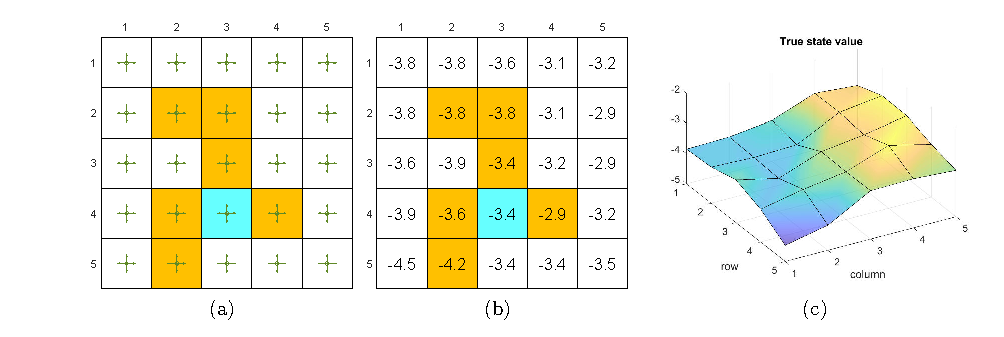
\includegraphics[width=441.6pt]{fig8_6}\par\smallskip
  \begin{minipage}{0.94\textwidth}\footnotesize
  \textbf{Figure 8.6.} (a) The policy to be evaluated. (b) The true state values are represented as a table. (c) The true state values are represented as a 3D surface.\par\smallskip
  \textcolor{rulegray}{\scriptsize Reproduced from S.~Zhao, \emph{Mathematical Foundations of Reinforcement Learning} (Springer, 2025).}
  \end{minipage}
\end{figure}


\subsection{Choosing features, with numbers}

\bk{\S8.2.3--8.2.4, pp.~162--167; Figures 8.6--8.8, pp.~164--167}

\begin{worked}{approximating 25 state values with fewer than 25 numbers \bkin{\S8.2.4, pp.~164--167}}
\textbf{Setup.} $5\times5$ grid; the policy takes each action with probability $0.2$;
$r_{\text{forbidden}}=r_{\text{boundary}}=-1$, $r_{\text{target}}=1$, $\gamma=0.9$;
$500$ episodes of $500$ steps each; $w$ initialised from a standard normal. The true
state values form a bumpy surface with entries such as $-3.8,-3.8,-3.6,-3.1,-3.2$ in
row 1 and $-4.5,-4.2,-3.4,-3.4,-3.5$ in row 5 \bkin{Figure 8.6(b), p.~164}.

\textbf{Polynomial features.} Let $x,y$ be the normalised column and row indices in
$[-1,1]$.
\begin{itemize}
  \item $\phi(s)=[x,y]^{\!\top}\in\R^2$ gives $\hat v=w_1x+w_2y$: a plane
        \emph{through the origin}. Too restrictive, since the true surface does not
        pass through the origin.
  \item $\phi(s)=[1,x,y]^{\!\top}\in\R^3$ \bkin{equation (8.15), p.~165} gives a
        general plane. Result: the RMSE falls and then \emph{plateaus} --- a plane
        cannot bend \bkin{Figure 8.7(a), p.~166}.
  \item $\phi(s)=[1,x,y,x^2,y^2,xy]^{\!\top}\in\R^6$ \bkin{equation (8.16)}: a
        quadratic surface. Lower plateau.
  \item $\phi(s)=[1,x,y,x^2,y^2,xy,x^3,y^3,x^2y,xy^2]^{\!\top}\in\R^{10}$
        \bkin{equation (8.17)}: lower still.
\end{itemize}
\textbf{In all three cases the error plateaus above zero.} More features means less
bias, but a linear approximator of fixed dimension has a floor it cannot go below
\bkin{\S8.2.4, p.~166}.

\textbf{Fourier features.} Normalise $x,y$ into $[0,1]$ and use
\bkin{equation (8.18), p.~167}
\[
  \phi(s)=\Bigl[\ \vdots\ ,\ \cos\bigl(\pi(c_1x+c_2y)\bigr),\ \vdots\ \Bigr]^{\!\top}\in\R^{(q+1)^2},
  \qquad c_1,c_2\in\{0,1,\dots,q\}.
\]
For $q=1$:
$\phi(s)=[1,\ \cos(\pi y),\ \cos(\pi x),\ \cos(\pi(x+y))]^{\!\top}\in\R^4$. Taking
$q=1,2,3$ gives feature dimensions $4,9,16$ and monotonically better accuracy
\bkin{Figure 8.8, p.~167}.

Note $\pi$ here is the circle constant, not a policy --- the book flags the clash
\bkin{p.~167}.
\end{worked}

\begin{figure}[htbp]
  \centering
  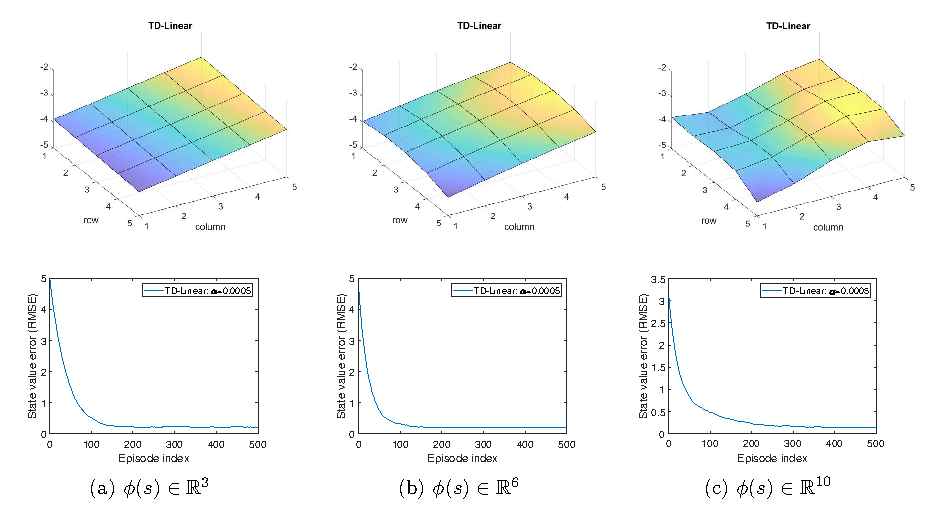
\includegraphics[width=441.6pt]{fig8_7}\par\smallskip
  \begin{minipage}{0.94\textwidth}\footnotesize
  \textbf{Figure 8.7.} TD-Linear estimation results obtained with the polynomial features in (8.15), (8.16), and (8.17).\par\smallskip
  \textcolor{rulegray}{\scriptsize Reproduced from S.~Zhao, \emph{Mathematical Foundations of Reinforcement Learning} (Springer, 2025).}
  \end{minipage}
\end{figure}


\begin{figure}[htbp]
  \centering
  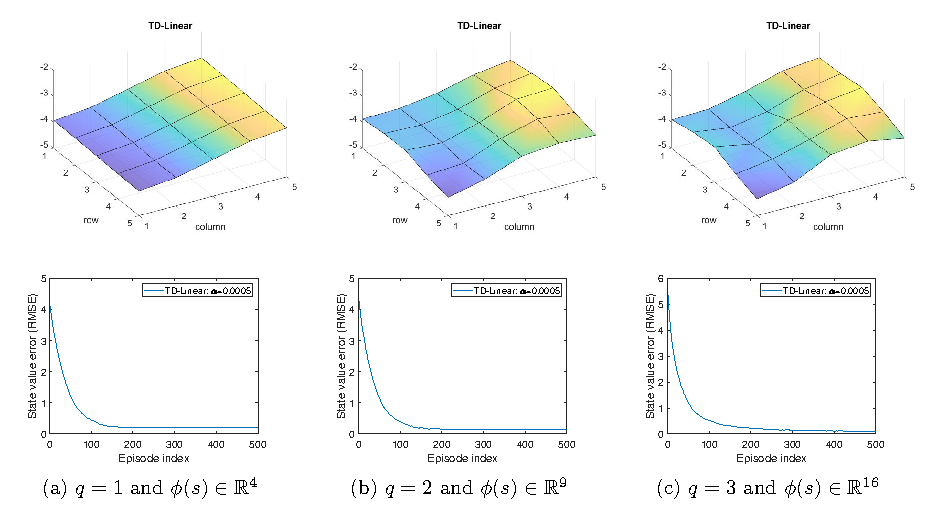
\includegraphics[width=441.6pt]{fig8_8}\par\smallskip
  \begin{minipage}{0.94\textwidth}\footnotesize
  \textbf{Figure 8.8.} TD-Linear estimation results obtained with the Fourier features in (8.18).\par\smallskip
  \textcolor{rulegray}{\scriptsize Reproduced from S.~Zhao, \emph{Mathematical Foundations of Reinforcement Learning} (Springer, 2025).}
  \end{minipage}
\end{figure}


\subsection{What is TD with function approximation actually minimising?}

\bk{\S8.2.5, pp.~167--178}

Here is an uncomfortable fact the book states plainly: \textbf{the algorithm (8.13)
does not minimise the objective function (8.3) it was derived from}
\bkin{\S8.2.5, p.~168}. The derivation was heuristic (we substituted an estimate for
$v_\pi$ mid-derivation). So what \emph{does} it do? The linear case can be answered
completely.

\subsubsection{Convergence}

\bk{\S8.2.5, pp.~168--169; Lemma 8.1, p.~168; equations (8.20)--(8.22)}

Consider the deterministic (expected) version \bkin{equation (8.19), p.~168}:
\[
  w_{t+1}=w_t+\alpha_t\E\bigl[\bigl(r_{t+1}+\gamma\phi^{\!\top}(s_{t+1})w_t-\phi^{\!\top}(s_t)w_t\bigr)\phi(s_t)\bigr],
\]
where $s_t\sim d_\pi$. Define \bkin{equation (8.20), p.~168}
\[
  \Phi=\begin{bmatrix}\vdots\\ \phi^{\!\top}(s)\\ \vdots\end{bmatrix}\in\R^{n\times m},
  \qquad
  D=\mathrm{diag}\bigl(d_\pi(s)\bigr)\in\R^{n\times n}.
\]

\begin{lemma}[Lemma 8.1, p.~168; equation (8.21)]
\[
  \E\bigl[(r_{t+1}+\gamma\phi^{\!\top}(s_{t+1})w_t-\phi^{\!\top}(s_t)w_t)\phi(s_t)\bigr]=b-Aw_t,
\]
where
\[
  A\doteq\Phi^{\!\top}D(I-\gamma P_\pi)\Phi\in\R^{m\times m},
  \qquad
  b\doteq\Phi^{\!\top}Dr_\pi\in\R^m .
\]
\end{lemma}

So the deterministic algorithm is simply
$w_{t+1}=w_t+\alpha_t(b-Aw_t)$ \bkin{equation (8.22), p.~169} --- a linear recursion
whose only possible fixed point is
\[
  \boxed{\;w^*=A^{-1}b.\;}
\]

\begin{theorem}[Positive definiteness of $A$, Box 8.4, pp.~171--173]
$A=\Phi^{\!\top}D(I-\gamma P_\pi)\Phi$ is positive definite, hence invertible.
\end{theorem}

\begin{proof}[Proof idea]
Set $M=D(I-\gamma P_\pi)$; it suffices that $M\succ0$, since $\Phi$ has full column
rank when the features are linearly independent. Because
$x^{\!\top}(M-M^{\!\top})x=0$, $M\succ0$ iff $M+M^{\!\top}\succ0$. Now use
$P_\pi\mathbf 1_n=\mathbf 1_n$ and $P_\pi^{\!\top}d_\pi=d_\pi$ to get
\[
  (M+M^{\!\top})\mathbf 1_n=2(1-\gamma)d_\pi>0,
\]
using $d_\pi(s)>0$ for all $s$ (Box 8.1). Since $M$ has positive diagonal and
nonpositive off-diagonal entries, this says $M+M^{\!\top}$ is strictly diagonally
dominant, and strictly diagonally dominant matrices are positive definite.
\end{proof}

\begin{remark}[Two proofs of convergence \bkin{\S8.2.5, pp.~169--170}]
\emph{Proof 1.} With $\delta_t=w_t-w^*$ and constant $\alpha$,
$\delta_{t+1}=(I-\alpha A)\delta_t$, so
$\norm{\delta_{t+1}}_2\le\norm{I-\alpha A}_2^{t+1}\norm{\delta_0}_2$, and
$\norm{I-\alpha A}_2<1$ for small $\alpha>0$ because $A\succ0$.

\emph{Proof 2.} With $g(w)=b-Aw$, finding $w^*$ is a root-finding problem and
(8.22) is a Robbins--Monro algorithm --- Chapter 6 again, now applied to a
deterministic process.
\end{remark}

\begin{worked}{the tabular case recovered exactly \bkin{equation (8.23), p.~169}}
Take $\phi(s)=e_s$, so $\Phi=I$. Then $A=D(I-\gamma P_\pi)$ and $b=Dr_\pi$, hence
\[
  w^*=A^{-1}b=(I-\gamma P_\pi)^{-1}D^{-1}Dr_\pi=(I-\gamma P_\pi)^{-1}r_\pi=v_\pi .
\]
The learned parameter vector \emph{is} the true state value vector --- consistent
with Box 8.2.
\end{worked}

\subsubsection{Three objective functions}

\bk{\S8.2.5, pp.~173--175; equation (8.30); Box 8.5, pp.~174--175}

\begin{itemize}
  \item \textbf{Value error} $J_E(w)=\norm{\hat v(w)-v_\pi}_D^2$, where
        $\norm{x}_D^2=x^{\!\top}Dx$. The natural objective --- but it needs the
        unknown $v_\pi$.
  \item \textbf{Bellman error}
        $J_{BE}(w)=\norm{\hat v(w)-T_\pi(\hat v(w))}_D^2$ with the Bellman operator
        $T_\pi(x)\doteq r_\pi+\gamma P_\pi x$ \bkin{equation (8.30), p.~173}.
        Implementable, but generally \emph{cannot be driven to zero}: the true
        $v_\pi$ may lie outside the span of your approximator.
  \item \textbf{Projected Bellman error}
        $J_{PBE}(w)=\norm{\hat v(w)-MT_\pi(\hat v(w))}_D^2$, where
        $M=\Phi(\Phi^{\!\top}D\Phi)^{-1}\Phi^{\!\top}D$ projects orthogonally onto
        the span of $\Phi$. \textbf{This one can always be driven to zero}, because
        both sides then live in the same subspace.
\end{itemize}

\begin{theorem}[Box 8.5, pp.~174--175]
$w^*=A^{-1}b=\argmin_w J_{PBE}(w)$.
\end{theorem}

\begin{proof}[Proof]
$J_{PBE}(w)=0\iff\Phi w=M T_\pi(\Phi w)$. Substituting $M$ and using that $\Phi$ has
full column rank,
\[
  w=(\Phi^{\!\top}D\Phi)^{-1}\Phi^{\!\top}D(r_\pi+\gamma P_\pi\Phi w)
  \iff \Phi^{\!\top}Dr_\pi=\Phi^{\!\top}D(I-\gamma P_\pi)\Phi w
  \iff w=A^{-1}b .
\]
\end{proof}

\begin{intuition}[What the projection means]
Your approximator can only produce values in the range of $\Phi$ --- a
low-dimensional subspace. Applying the Bellman operator generally throws you out of
that subspace. So you cannot ask for $\hat v=T_\pi(\hat v)$; the best you can ask is
that $\hat v$ equal the \emph{projection back} of $T_\pi(\hat v)$. TD learning finds
that fixed point. It is the RL analogue of ``the OLS residual is orthogonal to the
regressor space''.
\end{intuition}

\begin{theorem}[Error bound, equation (8.32), p.~176; proof in Box 8.6]
\[
  \norm{\hat v(w^*)-v_\pi}_D\ \le\ \frac{1}{1-\gamma}\min_w\norm{\hat v(w)-v_\pi}_D
  =\frac{1}{1-\gamma}\min_w\sqrt{J_E(w)} .
\]
\end{theorem}

\begin{remark}
The right-hand side is the best your approximator class could possibly do, inflated
by $1/(1-\gamma)$. The book is candid: this bound is \textbf{loose}, especially when
$\gamma$ is near one (at $\gamma=0.9$ the factor is $10$), and is mainly of
theoretical value \bkin{\S8.2.5, p.~176}.
\end{remark}

\subsubsection{Least-squares TD}

\bk{\S8.2.5, pp.~177--178; equation (8.34)}

$A$ and $b$ are themselves expectations \bkin{p.~177}:
\[
  A=\E\bigl[\phi(s_t)(\phi(s_t)-\gamma\phi(s_{t+1}))^{\!\top}\bigr],
  \qquad
  b=\E\bigl[r_{t+1}\phi(s_t)\bigr].
\]
So estimate them by sample averages and invert once
\bkin{equation (8.34), p.~177}:
\[
  \hat A_t=\sum_{k=0}^{t-1}\phi(s_k)\bigl(\phi(s_k)-\gamma\phi(s_{k+1})\bigr)^{\!\top},
  \qquad
  \hat b_t=\sum_{k=0}^{t-1}r_{k+1}\phi(s_k),
  \qquad
  w_t=\hat A_t^{-1}\hat b_t .
\]
The $1/t$ factors cancel and are omitted. In practice $\hat A_t$ is regularised as
$\hat A_t+\sigma I$ for small $\sigma$, since it may be singular for small $t$
\bkin{p.~178}. LSTD uses data more efficiently than TD-Linear but requires a matrix
inverse and works only in the linear case.

\subsection{Sarsa and Q-learning with function approximation}

\bk{\S8.3, pp.~179--181; equations (8.35)--(8.36); Algorithms 8.2--8.3, pp.~180--181}

The extension is mechanical: replace $\hat v(s,w)$ with $\hat q(s,a,w)$.

\begin{definition}[Sarsa with function approximation, equation (8.35), p.~179]
\[
  w_{t+1}=w_t+\alpha_t\bigl[r_{t+1}+\gamma\hat q(s_{t+1},a_{t+1},w_t)-\hat q(s_t,a_t,w_t)\bigr]
    \nabla_w\hat q(s_t,a_t,w_t).
\]
In the linear case $\hat q(s,a,w)=\phi^{\!\top}(s,a)w$ and
$\nabla_w\hat q=\phi(s,a)$.
\end{definition}

\begin{definition}[Q-learning with function approximation, equation (8.36), p.~180]
\[
  w_{t+1}=w_t+\alpha_t\Bigl[r_{t+1}+\gamma\max_{a\in\Aspace(s_{t+1})}\hat q(s_{t+1},a,w_t)-\hat q(s_t,a_t,w_t)\Bigr]
    \nabla_w\hat q(s_t,a_t,w_t).
\]
\end{definition}

\begin{algobox}{Sarsa with function approximation (Algorithm 8.2, p.~180)}
\textbf{Initialise:} $w_0$; $\pi_0$; $\alpha>0$; $\varepsilon\in(0,1)$.\\
For each episode: generate $a_0$ at $s_0$ from $\pi_0$; while $s_t$ is not the target:
\begin{itemize}\itemsep0pt
  \item Obtain $r_{t+1},s_{t+1}$ from the environment; draw $a_{t+1}\sim\pi_t(s_{t+1})$.
  \item $w_{t+1}=w_t+\alpha_t[r_{t+1}+\gamma\hat q(s_{t+1},a_{t+1},w_t)-\hat q(s_t,a_t,w_t)]\nabla_w\hat q(s_t,a_t,w_t)$.
  \item Set $\pi_{t+1}(\cdot\mid s_t)$ to be $\varepsilon$-greedy w.r.t.\ $\hat q(s_t,\cdot,w_{t+1})$.
  \item $s_t\leftarrow s_{t+1},\ a_t\leftarrow a_{t+1}$.
\end{itemize}
\end{algobox}

\begin{worked}{results on the grid world \bkin{Figures 8.9--8.10, pp.~180--181}}
Both use Fourier features of order $5$, with $\gamma=0.9$, $\varepsilon=0.1$,
$r_{\text{boundary}}=r_{\text{forbidden}}=-10$, $r_{\text{target}}=1$,
$\alpha=0.001$. Over $500$ episodes the total reward rises from around $-4000$
toward $0$ and the episode length falls, in both Sarsa and Q-learning. Both find a
good path from the top-left state.
\end{worked}

\begin{warning}
In Algorithms 8.2 and 8.3 the \emph{values} are functions but the \emph{policy} is
still a table --- $\pi(a\mid s)$ is stored per state and updated per state. So the
state and action spaces must still be finite. Removing that last table is the entire
subject of Chapter 9 \bkin{\S8.3.2, p.~181}.
\end{warning}

\begin{figure}[htbp]
  \centering
  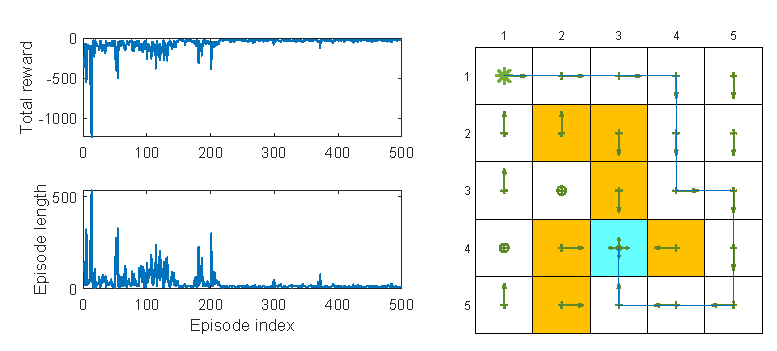
\includegraphics[width=372.8pt]{fig8_9}\par\smallskip
  \begin{minipage}{0.94\textwidth}\footnotesize
  \textbf{Figure 8.9.} Sarsa with linear function approximation. Here, $\gamma$ = 0.9, $\varepsilon$ = 0.1, rboundary = rforbidden = $-$10, rtarget = 1, and $\alpha$ = 0.001.\par\smallskip
  \textcolor{rulegray}{\scriptsize Reproduced from S.~Zhao, \emph{Mathematical Foundations of Reinforcement Learning} (Springer, 2025).}
  \end{minipage}
\end{figure}


\begin{figure}[htbp]
  \centering
  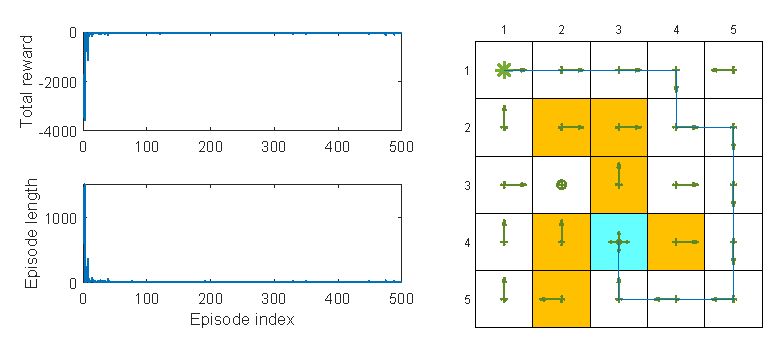
\includegraphics[width=372.8pt]{fig8_10}\par\smallskip
  \begin{minipage}{0.94\textwidth}\footnotesize
  \textbf{Figure 8.10.} Q-learning with linear function approximation. Here, $\gamma$ = 0.9, $\varepsilon$ = 0.1, rboundary = rforbidden = $-$10, rtarget = 1, and $\alpha$ = 0.001.\par\smallskip
  \textcolor{rulegray}{\scriptsize Reproduced from S.~Zhao, \emph{Mathematical Foundations of Reinforcement Learning} (Springer, 2025).}
  \end{minipage}
\end{figure}


\subsection{Deep Q-learning (DQN)}

\bk{\S8.4, pp.~181--186; equations (8.37)--(8.38); Algorithm 8.3, p.~183}

\begin{definition}[DQN objective, equation (8.37), p.~182]
\[
  J=\E\Bigl[\Bigl(R+\gamma\max_{a\in\Aspace(S')}\hat q(S',a,w)-\hat q(S,A,w)\Bigr)^2\Bigr],
\]
the \textbf{squared Bellman optimality error}.
\end{definition}

The justification: the Bellman optimality equation in action-value form
(Box 7.5, p.~140) says the bracket is zero in expectation when $\hat q$ is exact.

\subsubsection{Trick 1: two networks}

\bk{\S8.4.1, pp.~182--183}

The parameter $w$ appears \emph{twice} --- inside $\hat q(S,A,w)$ and inside the
target $y=R+\gamma\max_a\hat q(S',a,w)$ --- which makes the gradient awkward. DQN
freezes the copy inside the target:

\begin{itemize}
  \item a \textbf{main network} $\hat q(s,a,w)$, updated every iteration;
  \item a \textbf{target network} $\hat q(s,a,w_T)$, held fixed and refreshed by
        $w_T\leftarrow w$ every $C$ iterations.
\end{itemize}
With $w_T$ fixed, \bkin{equation (8.38), p.~182}
\[
  \nabla_wJ=-\E\Bigl[\Bigl(R+\gamma\max_{a}\hat q(S',a,w_T)-\hat q(S,A,w)\Bigr)\nabla_w\hat q(S,A,w)\Bigr].
\]

\begin{intuition}
Without the frozen copy you are chasing a target that moves every time you step
toward it --- the classic recipe for instability. Freezing $w_T$ for $C$ iterations
turns each phase into an ordinary supervised regression with fixed labels.
\end{intuition}

\subsubsection{Trick 2: experience replay}

\bk{\S8.4.1, pp.~183--184}

Store transitions $(s,a,r,s')$ in a \textbf{replay buffer}
$\mathcal B$, and each update draw a \emph{mini-batch uniformly at random} from
$\mathcal B$ rather than using samples in the order they arrived.

\begin{remark}[The book's reason, which is not the usual folklore]
\bkin{\S8.4.1, pp.~183--184; \S8.6 Q\&A, p.~187} Look back at the objective (8.37).
To define that expectation we must specify the distribution of $(S,A)$. The
distributions of $R$ and $S'$ follow from the model once $(S,A)$ is given; for
$(S,A)$ the simplest assumption is \emph{uniform}. But samples generated
sequentially by a behaviour policy are neither uniform nor independent.
\textbf{Uniform sampling from the replay buffer is what makes the assumption behind
the objective function true.} A side benefit --- often quoted as the main one --- is
that each sample can be reused many times, which matters when data is scarce.
\end{remark}

\begin{remark}
Does tabular Q-learning need replay? \emph{No}, but it can use it, and it benefits
from the sample reuse \bkin{\S8.6 Q\&A, p.~187}.
\end{remark}

\begin{algobox}{Deep Q-learning, off-policy (Algorithm 8.3, p.~183)}
\textbf{Initialise:} a main network and a target network with identical parameters.\\
\textbf{Goal:} learn optimal action values from samples generated by a behaviour
policy $\pi_b$.\\
Store samples generated by $\pi_b$ in a replay buffer
$\mathcal B=\{(s,a,r,s')\}$. Then for each iteration:
\begin{itemize}\itemsep0pt
  \item Draw a mini-batch uniformly from $\mathcal B$.
  \item For each sample, compute the target
        $y_T=r+\gamma\max_{a\in\Aspace(s')}\hat q(s',a,w_T)$.
  \item Update the main network to minimise $\sum(y_T-\hat q(s,a,w))^2$ over the
        mini-batch (using standard neural-network training tools, not equation
        (8.38) directly).
  \item Every $C$ iterations, set $w_T\leftarrow w$.
\end{itemize}
\end{algobox}

\subsubsection{Two experiments, one encouraging and one sobering}

\bk{\S8.4.2, pp.~184--186; Figures 8.11--8.12, pp.~185--186}

\begin{worked}{DQN with 1{,}000 samples \bkin{Figure 8.11, p.~185}}
\textbf{Setup.} $5\times5$ grid, $\gamma=0.9$,
$r_{\text{boundary}}=r_{\text{forbidden}}=-10$, $r_{\text{target}}=1$. Behaviour
policy: uniform (probability $0.2$ on each action). \textbf{A single episode of
$1{,}000$ steps.} Replay buffer holds those $1{,}000$ transitions; mini-batch size
$100$.

\textbf{Network.} One hidden layer of $100$ neurons; three inputs (normalised row,
normalised column, normalised action index) and one output. The book notes the
design choice: feeding row and column rather than a flat state index tells the
network that states have a $2$-D geometry --- \emph{the more structure you encode,
the better the network performs} \bkin{p.~185}. An alternative is two inputs and
five outputs (one per action), as in the original DQN paper.

\textbf{Result.} The loss converges to zero and the state-value RMSE converges to
zero; the greedy policy extracted from the learned $\hat q$ is optimal.

\textbf{The headline comparison.} Tabular Q-learning needed an episode of
$100{,}000$ steps for the same task \bkin{Figure 7.4}; DQN needed $1{,}000$ --- a
hundredfold reduction. Two reasons \bkin{p.~185}: function approximation
generalises across states, and replay lets each sample be used many times.
\end{worked}

\begin{figure}[htbp]
  \centering
  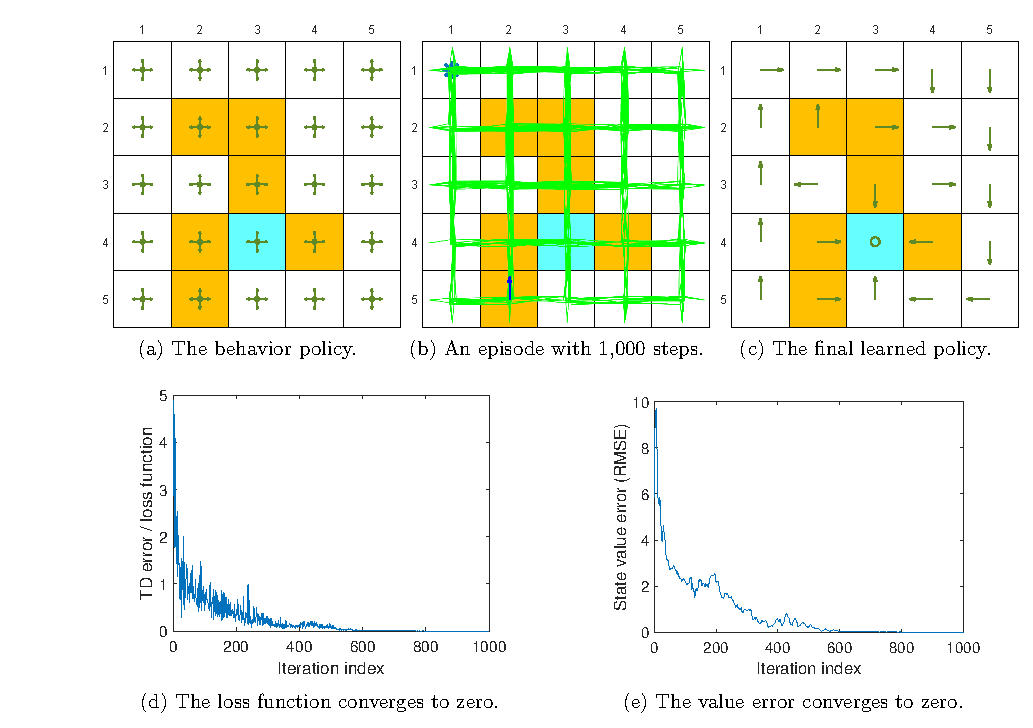
\includegraphics[width=441.6pt]{fig8_11}\par\smallskip
  \begin{minipage}{0.94\textwidth}\footnotesize
  \textbf{Figure 8.11.} Optimal policy learning via deep Q-learning. Here, $\gamma$ = 0.9, rboundary = rforbidden = $-$10, and rtarget = 1. The batch size is 100.\par\smallskip
  \textcolor{rulegray}{\scriptsize Reproduced from S.~Zhao, \emph{Mathematical Foundations of Reinforcement Learning} (Springer, 2025).}
  \end{minipage}
\end{figure}


\begin{worked}{DQN with 100 samples \bkin{Figure 8.12, p.~186}}
Same setup, but the episode is only $100$ steps and the mini-batch size is $50$.

\textbf{Result.} The loss function \emph{still} converges to zero --- but the
state-value RMSE plateaus around $5$ and never converges.

\textbf{Diagnosis.} The network fits the training samples perfectly and the optimal
action values badly. Zero training loss is not evidence of a correct value function;
it is evidence that you have enough parameters to memorise the data you have. Any
econometrician will recognise the phenomenon: in-sample fit is not identification.
\end{worked}

\begin{figure}[htbp]
  \centering
  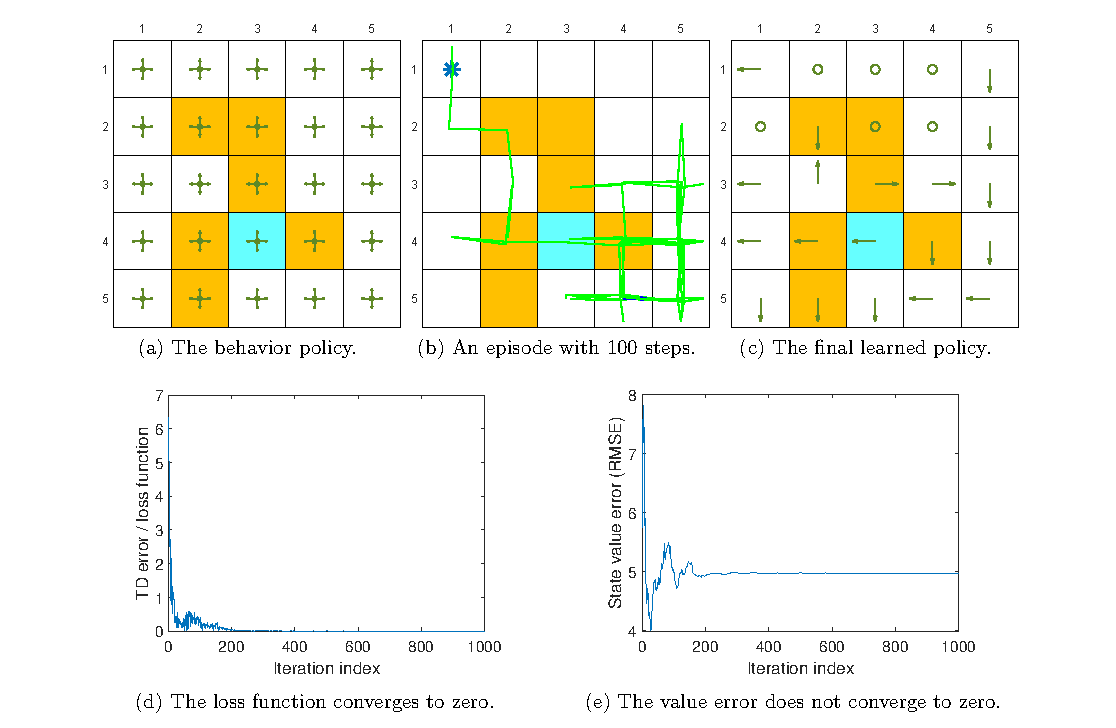
\includegraphics[width=441.6pt]{fig8_12}\par\smallskip
  \begin{minipage}{0.94\textwidth}\footnotesize
  \textbf{Figure 8.12.} Optimal policy learning via deep Q-learning. Here, $\gamma$ = 0.9, rboundary = rforbidden = $-$10, and rtarget = 1. The batch size is 50.\par\smallskip
  \textcolor{rulegray}{\scriptsize Reproduced from S.~Zhao, \emph{Mathematical Foundations of Reinforcement Learning} (Springer, 2025).}
  \end{minipage}
\end{figure}


\subsection{Chapter 8 summary and self-check}

\bk{\S8.5, pp.~186--187}

\begin{center}
\small
\begin{tabular}{@{}lp{0.62\textwidth}@{}}
\toprule
Concept & The point \\
\midrule
Table $\to$ function & Saves storage and, more importantly, generalises across states. Costs accuracy. \\
Stationary distribution $d_\pi$ & Weights the objective by how often each state is actually visited; exists and is positive for exploratory policies. \\
TD-Linear & $w_{t+1}=w_t+\alpha_t[r_{t+1}+\gamma\phi^{\!\top}(s_{t+1})w_t-\phi^{\!\top}(s_t)w_t]\phi(s_t)$; tabular TD is the case $\phi(s)=e_s$. \\
$w^*=A^{-1}b$ & The unique fixed point; it minimises the \emph{projected} Bellman error, not the value error. \\
DQN & Squared Bellman optimality error, minimised with a frozen target network and uniform experience replay. \\
\bottomrule
\end{tabular}
\end{center}

\begin{enumerate}
  \item Explain generalisation using Figure 8.4: why does a sample at $s_3$ change
        $\hat v(s_1)$ under function approximation but not under a table?
  \item Show that $\phi(s)=e_s$ turns TD-Linear into tabular TD.
  \item Why is the objective weighted by $d_\pi$ rather than uniformly? What property
        of the policy guarantees $d_\pi$ exists and is strictly positive?
  \item Distinguish $J_E$, $J_{BE}$ and $J_{PBE}$. Which one can always be driven to
        zero, and why?
  \item In the $\varepsilon=0.5$ example, verify that
        $d_\pi=[0.0345,0.1084,0.1330,0.7241]^{\!\top}$ satisfies
        $d_\pi^{\!\top}=d_\pi^{\!\top}P_\pi$ numerically.
  \item State the book's mathematical reason for uniform experience replay --- not the
        folklore reason.
  \item In Figure 8.12 the loss goes to zero but the value error does not. Explain
        the difference in one sentence.
\end{enumerate}

\newpage
% ============================================================
\section{Policy Gradient Methods}
% ============================================================

\begin{roadmap}{Chapter 9 of the textbook}
\textbf{Textbook:} Chapter 9, pp.~191--214. Sections: \S9.1 policy representation ---
from table to function (p.~192), \S9.2 metrics for defining optimal policies (p.~193),
\S9.3 gradients of the metrics (p.~198; discounted case p.~200, undiscounted case
p.~205), \S9.4 Monte Carlo policy gradient / REINFORCE (p.~210), \S9.5 summary
(p.~213), \S9.6 Q\&A (p.~213). Theorem 9.1 (p.~198), Lemmas 9.1--9.2 (p.~200),
Theorems 9.2--9.3 (pp.~201--203), Theorems 9.4--9.5 (pp.~205--209),
Algorithm 9.1 (p.~212). Table 9.2 (p.~197).\\[0.3em]
\textbf{Videos:}
\vid{L9 P1 --- Basic idea}{https://www.youtube.com/watch?v=mtFHOj83QSo};
\vid{L9 P2 --- Metric 1: average value}{https://www.youtube.com/watch?v=la8jQc3hX1M};
\vid{L9 P3 --- Metric 2: average reward}{https://www.youtube.com/watch?v=8RZ_rQFe69E};
\vid{L9 P4 --- Gradients of the metrics}{https://www.youtube.com/watch?v=MvmtPXur3Ls};
\vid{L9 P5 --- Gradient-based algorithms \& REINFORCE}{https://www.youtube.com/watch?v=1DQnnUC8ng8}.\\[0.3em]
\textbf{The break with everything before.} Chapters 1--8 are \emph{value-based}: learn
values, then read off a greedy policy. This chapter is \emph{policy-based}: parameterise
the policy directly and do gradient ascent on a scalar objective. Values become
optional.
\end{roadmap}

\begin{figure}[htbp]
  \centering
  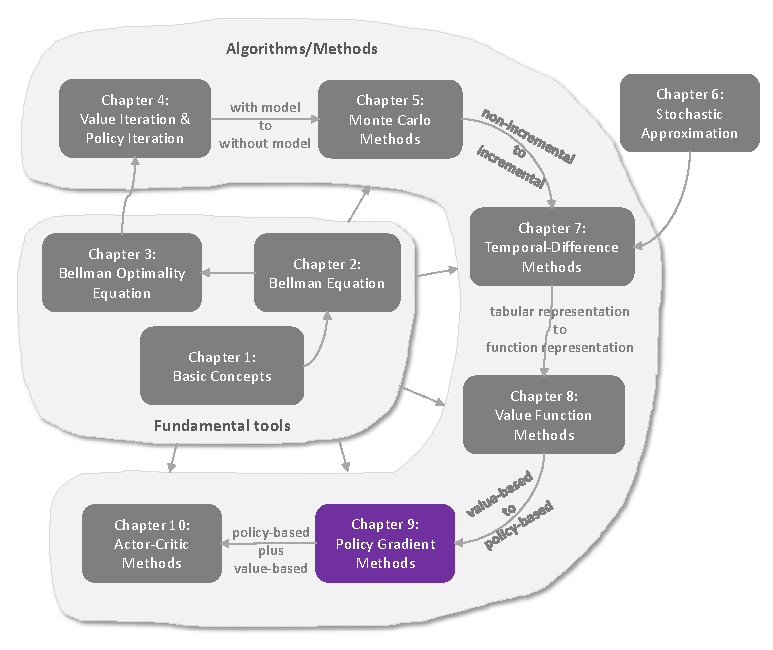
\includegraphics[width=371.3pt]{fig9_1}\par\smallskip
  \begin{minipage}{0.94\textwidth}\footnotesize
  \textbf{Figure 9.1.} Where we are in this book.\par\smallskip
  \textcolor{rulegray}{\scriptsize Reproduced from S.~Zhao, \emph{Mathematical Foundations of Reinforcement Learning} (Springer, 2025).}
  \end{minipage}
\end{figure}


\subsection{From a table of probabilities to a function}

\bk{\S9.1, pp.~192--193; Table 9.1 and Figure 9.2, p.~192}

Until now a policy was a table: one row per state, one column per action, holding
$\pi(a\mid s)$. Now write
\[
  \pi(a\mid s,\theta),\qquad \theta\in\R^m,
\]
also written $\pi_\theta(a\mid s)$. Three things change \bkin{\S9.1, p.~192}:

\begin{center}
\small
\begin{tabular}{@{}lll@{}}
\toprule
 & Tabular policy & Function policy \\
\midrule
Optimality means & maximise \emph{every} state value & maximise a chosen \emph{scalar metric} \\
Update by & rewriting table entries & changing $\theta$ \\
Retrieve $\pi(a\mid s)$ by & reading an entry & evaluating the function at $(s,a)$ \\
\bottomrule
\end{tabular}
\end{center}

\begin{warning}
The redefinition of optimality is the substantive change, not a technicality. With a
table you could demand dominance at every state simultaneously (Definition 3.1) and
Chapter 3 proved such a policy exists. With a parametric function you cannot: the
parameter budget forces trade-offs across states. So optimality must be defined by a
single number $J(\theta)$ \bkin{\S9.1, p.~192; \S3.7 Q\&A, p.~54}.
\end{warning}

\textbf{The method in one line} \bkin{\S9.1, p.~193}: pick a scalar metric $J(\theta)$
and run gradient \emph{ascent},
\[
  \theta_{t+1}=\theta_t+\alpha\nabla_\theta J(\theta_t).
\]
Three questions follow, and the chapter answers them in order: which metric
(\S9.2), what is its gradient (\S9.3), how do we estimate that gradient from samples
(\S9.4)?

\begin{figure}[htbp]
  \centering
  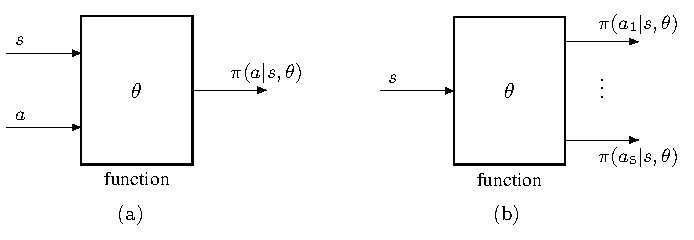
\includegraphics[width=332.9pt]{fig9_2}\par\smallskip
  \begin{minipage}{0.94\textwidth}\footnotesize
  \textbf{Figure 9.2.} Function representations of policies. The functions may have different structures.\par\smallskip
  \textcolor{rulegray}{\scriptsize Reproduced from S.~Zhao, \emph{Mathematical Foundations of Reinforcement Learning} (Springer, 2025).}
  \end{minipage}
\end{figure}


\subsection{Two metrics}

\bk{\S9.2, pp.~193--198; Table 9.2, p.~197}

\subsubsection{Metric 1: average state value}

\bk{\S9.2, pp.~193--195; equation (9.1)}

\begin{definition}
\[
  \bar v_\pi=\sum_{s\in\Sspace}d(s)v_\pi(s)=\E_{S\sim d}[v_\pi(S)]=d^{\!\top}v_\pi,
\]
where $d(s)\ge0$ and $\sum_sd(s)=1$.
\end{definition}

Two choices of the weights \bkin{\S9.2, pp.~193--194}:

\begin{itemize}
  \item \textbf{$d$ independent of $\pi$}, written $d_0$ and the metric $\bar v_\pi^0$.
        Either $d_0(s)=1/|\Sspace|$ (all states equally important), or, when there is
        a fixed starting state $s_0$, $d_0(s_0)=1$ and $d_0(s)=0$ elsewhere. The
        second case is common: ``how good is this policy when I start from home?''
  \item \textbf{$d=d_\pi$, the stationary distribution} (Box 8.1). States visited
        often in the long run get more weight. Note this makes the weights themselves
        depend on $\theta$, which will complicate the gradient.
\end{itemize}

\begin{remark}[An equivalent form you will meet elsewhere]
\bkin{equation (9.1), p.~194} The literature often writes
\[
  J(\theta)=\lim_{n\to\infty}\E\Bigl[\sum_{t=0}^n\gamma^tR_{t+1}\Bigr]
  =\E\Bigl[\sum_{t=0}^\infty\gamma^tR_{t+1}\Bigr].
\]
This looks different but equals $\bar v_\pi$: condition on $S_0$ and apply the law
of total expectation,
$\E[\sum_t\gamma^tR_{t+1}]=\sum_sd(s)\E[\sum_t\gamma^tR_{t+1}\mid S_0=s]=\sum_sd(s)v_\pi(s)$.
\end{remark}

\subsubsection{Metric 2: average reward}

\bk{\S9.2, pp.~195--197; equations (9.2)--(9.5); Box 9.1, pp.~196--197}

\begin{definition}[equations (9.2)--(9.3), p.~195]
\[
  \bar r_\pi\doteq\sum_{s\in\Sspace}d_\pi(s)r_\pi(s)=\E_{S\sim d_\pi}[r_\pi(S)],
  \qquad
  r_\pi(s)\doteq\sum_{a}\pi(a\mid s,\theta)r(s,a),
\]
with $r(s,a)\doteq\E[R\mid s,a]=\sum_r rp(r\mid s,a)$. In vector form
$\bar r_\pi=d_\pi^{\!\top}r_\pi$.
\end{definition}

\begin{remark}[An equivalent form, equations (9.4)--(9.5), p.~195]
\[
  J(\theta)=\lim_{n\to\infty}\frac1n\E\Bigl[\sum_{t=0}^{n-1}R_{t+1}\Bigr]=\bar r_\pi .
\]
The proof (Box 9.1, pp.~196--197) is a nice piece of probability: the Ces\`aro mean
lets you replace the average of a convergent sequence by its limit, so
$\lim_n\frac1n\E[\sum_tR_{t+1}\mid S_0=s_0]=\lim_t\E[R_{t+1}\mid S_0=s_0]$; then
$\E[R_{t+1}\mid S_0=s_0]=\sum_s r_\pi(s)p^{(t)}(s\mid s_0)\to\sum_s r_\pi(s)d_\pi(s)=\bar r_\pi$
because $p^{(t)}(s\mid s_0)\to d_\pi(s)$. \textbf{The starting state washes out} ---
long-run average reward does not care where you began.
\end{remark}

\subsubsection{The two metrics are the same metric}

\begin{lemma}[Lemma 9.1, p.~200]
In the discounted case $\gamma\in(0,1)$,
\[
  \boxed{\;\bar r_\pi=(1-\gamma)\,\bar v_\pi.\;}
\]
\end{lemma}

\begin{proof}
Multiply the Bellman equation $v_\pi=r_\pi+\gamma P_\pi v_\pi$ on the left by
$d_\pi^{\!\top}$ and use $d_\pi^{\!\top}P_\pi=d_\pi^{\!\top}$:
\[
  \bar v_\pi=\bar r_\pi+\gamma d_\pi^{\!\top}P_\pi v_\pi=\bar r_\pi+\gamma d_\pi^{\!\top}v_\pi
  =\bar r_\pi+\gamma\bar v_\pi .
\]
\end{proof}

\begin{remark}
Since $(1-\gamma)>0$, maximising one maximises the other. You may pick whichever is
analytically convenient \bkin{\S9.2, p.~198}.
\end{remark}

\begin{center}
\small
\begin{tabular}{@{}llll@{}}
\toprule
Metric & Expression 1 & Expression 2 & Expression 3 \\
\midrule
$\bar v_\pi$ & $\sum_s d(s)v_\pi(s)$ & $\E_{S\sim d}[v_\pi(S)]$
   & $\lim_{n\to\infty}\E\bigl[\sum_{t=0}^n\gamma^tR_{t+1}\bigr]$\\[0.3em]
$\bar r_\pi$ & $\sum_s d_\pi(s)r_\pi(s)$ & $\E_{S\sim d_\pi}[r_\pi(S)]$
   & $\lim_{n\to\infty}\frac1n\E\bigl[\sum_{t=0}^{n-1}R_{t+1}\bigr]$\\
\bottomrule
\end{tabular}
\end{center}
\centerline{\small (The book's Table 9.2, p.~197.)}

\subsection{The policy gradient theorem}

\bk{\S9.3, pp.~198--200; Theorem 9.1, p.~198; equations (9.8)--(9.11)}

\begin{theorem}[Policy gradient theorem, Theorem 9.1, p.~198]
\[
  \nabla_\theta J(\theta)=\sum_{s\in\Sspace}\eta(s)\sum_{a\in\Aspace}
    \nabla_\theta\pi(a\mid s,\theta)\,q_\pi(s,a),
  \tag{9.8}
\]
and equivalently, in expectation form,
\[
  \boxed{\;
  \nabla_\theta J(\theta)=\E_{S\sim\eta,\ A\sim\pi(S,\theta)}
    \bigl[\nabla_\theta\ln\pi(A\mid S,\theta)\,q_\pi(S,A)\bigr].
  \;}
  \tag{9.9}
\]
\end{theorem}

\begin{remark}[What Theorem 9.1 is, precisely]
\bkin{\S9.3, pp.~198--199} It is a \emph{summary} of Theorems 9.2, 9.3 and 9.5, which
handle different metrics ($\bar v_\pi^0$, $\bar v_\pi$, $\bar r_\pi$) and the
discounted versus undiscounted cases. Depending on the case, $\eta$ is either
$\rho_\pi$ or $d_\pi$, and the equality may be exact or approximate. The book is
explicit that most readers should learn the statement and skip the proofs.
\end{remark}

\begin{worked}{why the logarithm appears \bkin{\S9.3, p.~199; equations (9.10)--(9.11)}}
Rewrite (9.8) as an expectation over states:
\[
  \nabla_\theta J(\theta)=\E_{S\sim\eta}\Bigl[\sum_a\nabla_\theta\pi(a\mid S,\theta)q_\pi(S,a)\Bigr].
\]
The inner sum is not yet an expectation over actions, because the summand has no
factor $\pi(a\mid s,\theta)$. Manufacture one using the derivative of a logarithm:
\[
  \nabla_\theta\ln\pi(a\mid s,\theta)=\frac{\nabla_\theta\pi(a\mid s,\theta)}{\pi(a\mid s,\theta)}
  \quad\Longrightarrow\quad
  \nabla_\theta\pi(a\mid s,\theta)=\pi(a\mid s,\theta)\nabla_\theta\ln\pi(a\mid s,\theta).
\]
Substituting,
\[
  \nabla_\theta J(\theta)
  =\E_{S\sim\eta}\Bigl[\sum_a\pi(a\mid S,\theta)\nabla_\theta\ln\pi(a\mid S,\theta)q_\pi(S,a)\Bigr]
  =\E_{S\sim\eta,A\sim\pi}\bigl[\nabla_\theta\ln\pi(A\mid S,\theta)q_\pi(S,A)\bigr].
\]
\textbf{That is the entire role of the logarithm}: it converts a weighted sum into
an expectation, so the gradient can be estimated by sampling
\bkin{\S9.6 Q\&A, p.~214}. This is the ``log-derivative trick'', and it is the same
manoeuvre used to derive the score function in maximum likelihood estimation.
\end{worked}

\begin{warning}[The policy must be strictly positive]
$\ln\pi(a\mid s,\theta)$ requires $\pi(a\mid s,\theta)>0$ for every $(s,a)$
\bkin{\S9.3, p.~199}. The standard construction is the \textbf{softmax}
\bkin{equation (9.12), p.~199}:
\[
  \pi(a\mid s,\theta)=\frac{e^{h(s,a,\theta)}}{\sum_{a'\in\Aspace}e^{h(s,a',\theta)}},
\]
where $h(s,a,\theta)$ is a preference for taking $a$ at $s$. This guarantees
$\pi(a\mid s,\theta)\in(0,1)$ and $\sum_a\pi(a\mid s,\theta)=1$, and is implemented
as a network with a softmax output layer.

An important consequence \bkin{p.~199}: \textbf{the policy is automatically
stochastic and therefore automatically exploratory}. There is no $\varepsilon$ to
tune --- exploration is built into the representation. (Economists will recognise the
softmax as the choice probability of a multinomial logit model, with $h$ playing the
role of deterministic utility.)
\end{warning}

\subsubsection{Sketch of the derivation, discounted case}

\bk{\S9.3.1, pp.~200--205; Lemma 9.2, p.~200; Theorems 9.2--9.3, pp.~201--203}

\begin{lemma}[Gradient of a single state value, Lemma 9.2, p.~200; equation (9.14)]
\[
  \nabla_\theta v_\pi(s)=\sum_{s'\in\Sspace}\mathrm{Pr}_\pi(s'\mid s)
    \sum_{a\in\Aspace}\nabla_\theta\pi(a\mid s',\theta)q_\pi(s',a),
\]
where
$\mathrm{Pr}_\pi(s'\mid s)\doteq\sum_{k=0}^\infty\gamma^k[P_\pi^k]_{ss'}=[(I-\gamma P_\pi)^{-1}]_{ss'}$
is the \textbf{discounted total probability} of ever reaching $s'$ from $s$.
\end{lemma}

\begin{proof}[Proof idea (Box 9.2, pp.~201--202)]
Differentiate $v_\pi(s)=\sum_a\pi(a\mid s,\theta)q_\pi(s,a)$ by the product rule:
\[
  \nabla_\theta v_\pi(s)=\sum_a\bigl[\nabla_\theta\pi(a\mid s,\theta)q_\pi(s,a)
    +\pi(a\mid s,\theta)\nabla_\theta q_\pi(s,a)\bigr].
\]
Because $q_\pi(s,a)=r(s,a)+\gamma\sum_{s'}p(s'\mid s,a)v_\pi(s')$ and $r(s,a)$ does
not depend on $\theta$, we get
$\nabla_\theta q_\pi(s,a)=\gamma\sum_{s'}p(s'\mid s,a)\nabla_\theta v_\pi(s')$. So
$\nabla_\theta v_\pi$ appears on both sides --- bootstrapping again. Writing it in
matrix form and inverting gives the $(I-\gamma P_\pi)^{-1}$ factor.
\end{proof}

\begin{theorem}[Gradient of $\bar v_\pi^0$, Theorem 9.2, p.~201]
\[
  \nabla_\theta\bar v_\pi^0=\E\bigl[\nabla_\theta\ln\pi(A\mid S,\theta)q_\pi(S,A)\bigr],
  \quad S\sim\rho_\pi,\ A\sim\pi(S,\theta),
\]
where
$\rho_\pi(s)=\sum_{s'}d_0(s')\mathrm{Pr}_\pi(s\mid s')$ \bkin{equation (9.19), p.~201}.
\end{theorem}

\begin{theorem}[Gradients of $\bar r_\pi$ and $\bar v_\pi$, Theorem 9.3, p.~203]
\[
  \nabla_\theta\bar r_\pi=(1-\gamma)\nabla_\theta\bar v_\pi
  \ \approx\ \sum_s d_\pi(s)\sum_a\nabla_\theta\pi(a\mid s,\theta)q_\pi(s,a)
  =\E\bigl[\nabla_\theta\ln\pi(A\mid S,\theta)q_\pi(S,A)\bigr],
\]
with $S\sim d_\pi$, $A\sim\pi(S,\theta)$. \textbf{The approximation is more accurate
the closer $\gamma$ is to $1$.}
\end{theorem}

\begin{remark}[Where the approximation comes from]
Differentiating $\bar v_\pi=\sum_sd_\pi(s)v_\pi(s)$ produces two terms
\bkin{equation (9.20), p.~204}:
$\sum_s\nabla_\theta d_\pi(s)\,v_\pi(s)$ and $\sum_sd_\pi(s)\nabla_\theta v_\pi(s)$.
The second is the one we keep. The first --- the effect of $\theta$ on \emph{where the
agent spends its time} --- is what gets dropped. It is small when $\gamma\to1$.
\end{remark}

\begin{remark}[The undiscounted case]
\bkin{\S9.3.2, pp.~205--210; Theorems 9.4--9.5} For $\gamma=1$ the state value is no
longer well defined by the usual sum, and one works instead with the \textbf{Poisson
equation}, whose solution set is characterised by Theorem 9.4 (p.~205). The
conclusion, Theorem 9.5 (p.~209), is that $\nabla_\theta\bar r_\pi$ has the same
form as before --- but with an \emph{exact} equality rather than an approximation
\bkin{p.~209}. This is why the average-reward metric is worth defining separately:
it is valid in both the discounted and undiscounted settings
\bkin{\S9.6 Q\&A, p.~214}.
\end{remark}

\subsection{REINFORCE}

\bk{\S9.4, pp.~210--212; equations (9.31)--(9.33); Algorithm 9.1, p.~212}

Gradient ascent using the true gradient \bkin{equation (9.31), p.~210}:
\[
  \theta_{t+1}=\theta_t+\alpha\,\E\bigl[\nabla_\theta\ln\pi(A\mid S,\theta_t)q_\pi(S,A)\bigr].
\]
Replace the expectation by one sample (Chapter 6 again)
\bkin{equation (9.32), p.~211}:
\[
  \boxed{\;\theta_{t+1}=\theta_t+\alpha\,\nabla_\theta\ln\pi(a_t\mid s_t,\theta_t)\,q_t(s_t,a_t).\;}
\]
When $q_t(s_t,a_t)$ is obtained by Monte Carlo estimation --- i.e.\ the realised
discounted return from $(s_t,a_t)$ --- this is \textbf{REINFORCE}, also called Monte
Carlo policy gradient.

\subsubsection{Reading the update}

\bk{\S9.4, pp.~211--212; equation (9.33)}

Using $\nabla_\theta\ln\pi=\nabla_\theta\pi/\pi$, rewrite the update as
\[
  \theta_{t+1}=\theta_t+\alpha\underbrace{\frac{q_t(s_t,a_t)}{\pi(a_t\mid s_t,\theta_t)}}_{\beta_t}
    \nabla_\theta\pi(a_t\mid s_t,\theta_t)
  \qquad\Longleftrightarrow\qquad
  \theta_{t+1}=\theta_t+\alpha\beta_t\nabla_\theta\pi(a_t\mid s_t,\theta_t).
  \tag{9.33}
\]

\paragraph{Interpretation 1: it does the obvious thing.} A first-order Taylor
expansion gives \bkin{p.~211}
\[
  \pi(a_t\mid s_t,\theta_{t+1})\approx\pi(a_t\mid s_t,\theta_t)
   +\alpha\beta_t\norm{\nabla_\theta\pi(a_t\mid s_t,\theta_t)}_2^2 .
\]
So
\[
  \beta_t\ge0\ \Longrightarrow\ \pi(a_t\mid s_t,\theta_{t+1})\ge\pi(a_t\mid s_t,\theta_t),
  \qquad
  \beta_t<0\ \Longrightarrow\ \pi(a_t\mid s_t,\theta_{t+1})<\pi(a_t\mid s_t,\theta_t),
\]
and the size of the change scales with $|\beta_t|$. \emph{Actions that turned out
well become more likely; actions that turned out badly become less likely.}

\paragraph{Interpretation 2: exploration and exploitation, automatically.}
\bkin{p.~212} Look at $\beta_t=q_t(s_t,a_t)/\pi(a_t\mid s_t,\theta_t)$:

\begin{itemize}
  \item $\beta_t$ is \emph{proportional} to $q_t(s_t,a_t)$: high-value actions get
        reinforced. That is \textbf{exploitation}.
  \item $\beta_t$ is \emph{inversely proportional} to $\pi(a_t\mid s_t,\theta_t)$
        (when $q_t>0$): an action that currently has low probability gets a
        \emph{larger} boost when it turns out well. That is \textbf{exploration}.
\end{itemize}

\begin{intuition}
This is a strictly more elegant answer than $\varepsilon$-greedy. There, exploration
was bolted on with a tunable knob that had to be decayed by hand and that degraded
optimality (\S5.5). Here the trade-off falls out of the algebra of a single ratio.
\end{intuition}

\subsubsection{How the samples should be drawn}

\bk{\S9.4, p.~212}

\begin{itemize}
  \item \textbf{States:} $S$ should be drawn from $\eta$ --- either $d_\pi$ or
        $\rho_\pi$. Both describe long-run behaviour under $\pi$.
  \item \textbf{Actions:} $A$ should be drawn from $\pi(A\mid S,\theta)$.
        \textbf{Therefore the policy gradient method is on-policy.} You are
        estimating an expectation taken under $\pi$, so your data must come from
        $\pi$. (Chapter 10 shows how importance sampling relaxes this.)
\end{itemize}

\begin{remark}
The book is honest that the ideal sampling scheme is not followed in practice,
because it is too sample-inefficient \bkin{p.~212}. Algorithm 9.1 instead generates
one whole episode and then updates $\theta$ once per transition in it.
\end{remark}

\begin{algobox}{REINFORCE --- Monte Carlo policy gradient (Algorithm 9.1, p.~212)}
\textbf{Initialise:} $\theta$; $\gamma\in(0,1)$; $\alpha>0$.\\
\textbf{Goal:} learn a policy maximising $J(\theta)$.\\
For each episode:
\begin{itemize}\itemsep0pt
  \item Generate an episode $\{s_0,a_0,r_1,\dots,s_{T-1},a_{T-1},r_T\}$ following
        $\pi(\theta)$.
  \item For $t=0,1,\dots,T-1$:
    \begin{itemize}\itemsep0pt
      \item \textbf{Value update:}
            $q_t(s_t,a_t)=\sum_{k=t+1}^{T}\gamma^{\,k-t-1}r_k$
      \item \textbf{Policy update:}
            $\theta\leftarrow\theta+\alpha\nabla_\theta\ln\pi(a_t\mid s_t,\theta)\,q_t(s_t,a_t)$
    \end{itemize}
\end{itemize}
\end{algobox}

\begin{worked}{REINFORCE on a two-action state, by hand}
Suppose $\Aspace=\{a_1,a_2\}$ and a softmax policy with preferences
$h(s,a_1,\theta)=\theta_1$, $h(s,a_2,\theta)=\theta_2$, so
\[
  \pi(a_1\mid s,\theta)=\frac{e^{\theta_1}}{e^{\theta_1}+e^{\theta_2}} .
\]
Take $\theta=(0,0)$, so $\pi(a_1\mid s)=\pi(a_2\mid s)=0.5$. The score is
\[
  \nabla_\theta\ln\pi(a_1\mid s,\theta)
  =\bigl(1-\pi(a_1\mid s,\theta),\ -\pi(a_2\mid s,\theta)\bigr)=(0.5,\,-0.5).
\]
Suppose we sample $a_1$ and observe return $q_t=+2$. With $\alpha=0.1$,
\[
  \theta\leftarrow(0,0)+0.1(2)(0.5,-0.5)=(0.1,\,-0.1),
\]
giving $\pi(a_1\mid s)=e^{0.1}/(e^{0.1}+e^{-0.1})=0.550$. The probability of the
action that worked rose from $0.5$ to $0.55$; its rival fell to $0.45$. Had the
return been $-2$, the signs would flip and $\pi(a_1\mid s)$ would fall to $0.45$.
Note also that no explicit exploration parameter was needed --- the softmax keeps
both probabilities strictly positive forever.
\end{worked}

\subsection{Chapter 9 summary and self-check}

\bk{\S9.5, p.~213}

\begin{center}
\small
\begin{tabular}{@{}lp{0.60\textwidth}@{}}
\toprule
Item & The point \\
\midrule
Policy as a function & Optimality must be redefined via a scalar metric; policies are updated through $\theta$, not entry by entry. \\
$\bar v_\pi$ and $\bar r_\pi$ & Two metrics, equivalent in the discounted case via $\bar r_\pi=(1-\gamma)\bar v_\pi$. \\
Theorem 9.1 & $\nabla_\theta J=\E[\nabla_\theta\ln\pi(A\mid S,\theta)q_\pi(S,A)]$. The single most important result of the chapter. \\
The logarithm & A device to turn a weighted sum into an expectation, so it can be sampled. \\
Softmax policies & Guarantee $\pi>0$, making $\ln\pi$ valid and exploration automatic. \\
REINFORCE & $\theta\leftarrow\theta+\alpha\nabla_\theta\ln\pi(a_t\mid s_t,\theta)q_t(s_t,a_t)$ with $q_t$ a Monte Carlo return. \\
\bottomrule
\end{tabular}
\end{center}

\begin{enumerate}
  \item Why can optimality not be defined state-by-state once policies are
        parameterised?
  \item Prove $\bar r_\pi=(1-\gamma)\bar v_\pi$ in three lines.
  \item Derive $\nabla_\theta\pi=\pi\nabla_\theta\ln\pi$ and explain why it is the
        pivotal step in Theorem 9.1.
  \item Why must a softmax (or another strictly positive parameterisation) be used?
  \item Explain how $\beta_t=q_t/\pi$ balances exploration and exploitation, and
        contrast this with $\varepsilon$-greedy.
  \item Why is REINFORCE on-policy?
  \item Redo the two-action worked example with $\alpha=0.5$ and $q_t=-1$. What is
        the new $\pi(a_1\mid s)$?
\end{enumerate}

\newpage
% ============================================================
\section{Actor-Critic Methods}
% ============================================================

\begin{roadmap}{Chapter 10 of the textbook}
\textbf{Textbook:} Chapter 10, pp.~215--236. Sections: \S10.1 the simplest
actor-critic (QAC) (p.~216), \S10.2 advantage actor-critic (A2C) (p.~217; baseline
invariance p.~217, algorithm p.~220), \S10.3 off-policy actor-critic (p.~221;
importance sampling p.~221, off-policy policy gradient theorem p.~224, algorithm
p.~226), \S10.4 deterministic actor-critic (p.~227; the DPG theorem p.~227,
algorithm p.~234), \S10.5 summary (p.~235), \S10.6 Q\&A (p.~236). Algorithms 10.1
(p.~216), 10.2 (p.~220), 10.3 (p.~226), 10.4 (p.~234). Theorems 10.1--10.4.\\[0.3em]
\textbf{Videos:}
\vid{L10 P1 --- The simplest actor-critic}{https://www.youtube.com/watch?v=kjCZAT5Wh80};
\vid{L10 P2 --- Advantage actor-critic}{https://www.youtube.com/watch?v=vZVXJJcZNEM};
\vid{L10 P3 --- Importance sampling \& off-policy AC}{https://www.youtube.com/watch?v=TfO5mnsiGKc};
\vid{L10 P4 --- Deterministic actor-critic}{https://www.youtube.com/watch?v=dTjz1RNtic4}.\\[0.3em]
\textbf{The synthesis.} Chapters 1--8 were value-based, Chapter 9 was policy-based.
Actor-critic is both: the \emph{actor} updates the policy, the \emph{critic}
estimates the values the actor needs.
\end{roadmap}

\begin{figure}[htbp]
  \centering
  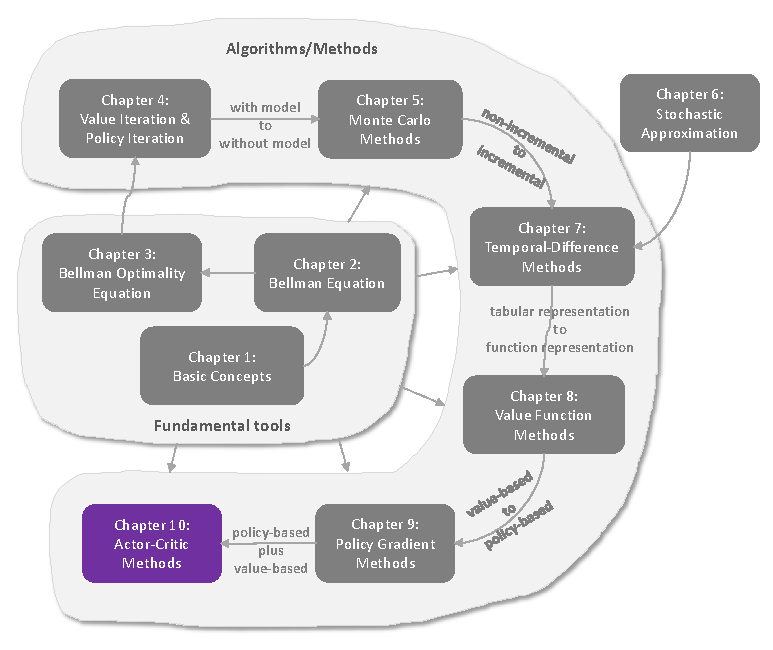
\includegraphics[width=371.3pt]{fig10_1}\par\smallskip
  \begin{minipage}{0.94\textwidth}\footnotesize
  \textbf{Figure 10.1.} Where we are in this book.\par\smallskip
  \textcolor{rulegray}{\scriptsize Reproduced from S.~Zhao, \emph{Mathematical Foundations of Reinforcement Learning} (Springer, 2025).}
  \end{minipage}
\end{figure}


\subsection{QAC: the simplest actor-critic}

\bk{\S10.1, pp.~216--217; equations (10.1)--(10.2); Algorithm 10.1, p.~216}

Start from the policy gradient update \bkin{equations (10.1)--(10.2), p.~216}:
\[
  \theta_{t+1}=\theta_t+\alpha\,\E_{S\sim\eta,A\sim\pi}\bigl[\nabla_\theta\ln\pi(A\mid S,\theta_t)q_\pi(S,A)\bigr]
  \ \longrightarrow\
  \theta_{t+1}=\theta_t+\alpha\nabla_\theta\ln\pi(a_t\mid s_t,\theta_t)q_t(s_t,a_t).
\]

\begin{intuition}[The observation that generates the whole chapter]
\bkin{\S10.1, p.~216} This one update is \emph{simultaneously} policy-based and
value-based. It updates the policy parameter directly --- policy-based. But it needs
$q_t(s_t,a_t)$, an estimate of an action value, which some value-based method must
supply. We know two ways to produce that estimate:
\begin{itemize}
  \item \textbf{Monte Carlo} $\Rightarrow$ REINFORCE (Chapter 9);
  \item \textbf{Temporal difference} $\Rightarrow$ \textbf{actor-critic}.
\end{itemize}
That is the definition. Actor-critic methods \emph{are} policy gradient methods in
which the action values come from TD learning with function approximation.
\end{intuition}

\begin{algobox}{Q actor-critic, QAC (Algorithm 10.1, p.~216)}
\textbf{Initialise:} a policy $\pi(a\mid s,\theta_0)$; a value function
$q(s,a,w_0)$; step sizes $\alpha_w,\alpha_\theta>0$.\\
At each time step $t$ of each episode:
\begin{itemize}\itemsep0pt
  \item Generate $a_t\sim\pi(\cdot\mid s_t,\theta_t)$; observe $r_{t+1},s_{t+1}$;
        generate $a_{t+1}\sim\pi(\cdot\mid s_{t+1},\theta_t)$.
  \item \textbf{Actor (policy update):}
        $\theta_{t+1}=\theta_t+\alpha_\theta\nabla_\theta\ln\pi(a_t\mid s_t,\theta_t)\,q(s_t,a_t,w_t)$
  \item \textbf{Critic (value update, Sarsa with function approximation):}
        $w_{t+1}=w_t+\alpha_w\bigl[r_{t+1}+\gamma q(s_{t+1},a_{t+1},w_t)-q(s_t,a_t,w_t)\bigr]\nabla_wq(s_t,a_t,w_t)$
\end{itemize}
\end{algobox}

\begin{remark}
The critic is exactly equation (8.35) --- Sarsa with function approximation. The actor
is exactly equation (9.32) --- the policy gradient update. Nothing new has been
invented; two existing pieces have been bolted together
\bkin{\S10.1, p.~216}.
\end{remark}

\subsection{Advantage actor-critic (A2C)}

\bk{\S10.2, pp.~217--221; equations (10.3)--(10.8); Algorithm 10.2, p.~220}

\subsubsection{Baseline invariance}

\bk{\S10.2.1, pp.~217--220; equation (10.3)}

\begin{theorem}[Baseline invariance, equation (10.3), p.~217]
For any scalar function $b(S)$ of the state alone,
\[
  \E_{S\sim\eta,A\sim\pi}\bigl[\nabla_\theta\ln\pi(A\mid S,\theta_t)q_\pi(S,A)\bigr]
  =\E_{S\sim\eta,A\sim\pi}\bigl[\nabla_\theta\ln\pi(A\mid S,\theta_t)\bigl(q_\pi(S,A)-b(S)\bigr)\bigr].
\]
\end{theorem}

\begin{proof}[Proof \bkin{\S10.2.1, pp.~217--218}]
It suffices that
$\E[\nabla_\theta\ln\pi(A\mid S,\theta_t)b(S)]=0$:
\[
\begin{aligned}
  \E\bigl[\nabla_\theta\ln\pi\,b(S)\bigr]
  &=\sum_s\eta(s)\sum_a\pi(a\mid s,\theta_t)\nabla_\theta\ln\pi(a\mid s,\theta_t)b(s)\\
  &=\sum_s\eta(s)b(s)\sum_a\nabla_\theta\pi(a\mid s,\theta_t)
   =\sum_s\eta(s)b(s)\,\nabla_\theta\underbrace{\sum_a\pi(a\mid s,\theta_t)}_{=1}
   =\sum_s\eta(s)b(s)\,\nabla_\theta 1=0 .
\end{aligned}
\]
\end{proof}

\begin{intuition}
The baseline is free because probabilities must sum to one, so the gradient of that
sum is zero. \emph{Anything that depends only on the state --- not on the action ---
cannot change which action the gradient favours.} It shifts every action's score by
the same amount.
\end{intuition}

\paragraph{So why bother?} Because the \emph{mean} is invariant but the
\emph{variance} is not \bkin{\S10.2.1, p.~218}. Let
\[
  X(S,A)\doteq\nabla_\theta\ln\pi(A\mid S,\theta_t)\bigl[q_\pi(S,A)-b(S)\bigr].
  \tag{10.4}
\]
The true gradient is $\E[X]$, estimated by a single draw $x$. If $\Var(X)$ is small,
any draw is a good estimate; if it is large, a draw can be wildly off. REINFORCE and
QAC use $b=0$, which is an arbitrary and generally poor choice.

\begin{theorem}[Optimal baseline, equation (10.5), p.~218; Box 10.1, p.~219]
\[
  b^*(s)=\frac{\E_{A\sim\pi}\bigl[\norm{\nabla_\theta\ln\pi(A\mid s,\theta_t)}^2q_\pi(s,A)\bigr]}
              {\E_{A\sim\pi}\bigl[\norm{\nabla_\theta\ln\pi(A\mid s,\theta_t)}^2\bigr]},
  \qquad s\in\Sspace .
\]
\end{theorem}

\begin{proof}[Proof idea (Box 10.1, p.~219)]
Minimise $\Tr[\Var(X)]=\E[X^{\!\top}X]-\bar x^{\!\top}\bar x$. Since $\bar x$ is
invariant, minimise
$\E[\norm{\nabla_\theta\ln\pi}^2(q_\pi(S,A)-b(S))^2]$. Setting the derivative in
$b(s)$ to zero gives a weighted-least-squares condition whose solution is $b^*$.
\end{proof}

\begin{remark}[The practical baseline]
$b^*$ is correct but too complicated to use. Drop the weight
$\norm{\nabla_\theta\ln\pi}^2$ and you get \bkin{p.~218}
\[
  b^\dagger(s)=\E_{A\sim\pi}[q_\pi(s,A)]=v_\pi(s).
\]
\textbf{The suboptimal-but-usable baseline is the state value.} This is a genuinely
pleasing result: the natural benchmark for ``was this action good?'' is ``compared to
the average action at this state''.
\end{remark}

\subsubsection{The advantage function}

\bk{\S10.2.2, pp.~220--221; equations (10.7)--(10.8)}

\begin{definition}[Advantage function]
\[
  \delta_\pi(S,A)\doteq q_\pi(S,A)-v_\pi(S).
\]
Because $v_\pi(s)=\sum_a\pi(a\mid s)q_\pi(s,a)$ is the mean of the action values,
$\delta_\pi(s,a)>0$ means $a$ is better than average at $s$
\bkin{\S10.2.2, p.~220}.
\end{definition}

The update becomes \bkin{equations (10.7)--(10.8), pp.~220}
\[
  \theta_{t+1}=\theta_t+\alpha\nabla_\theta\ln\pi(a_t\mid s_t,\theta_t)\bigl[q_t(s_t,a_t)-v_t(s_t)\bigr]
  =\theta_t+\alpha\nabla_\theta\ln\pi(a_t\mid s_t,\theta_t)\,\delta_t(s_t,a_t).
\]
If $q_t,v_t$ come from Monte Carlo, this is \emph{REINFORCE with a baseline}; if from
TD, it is \textbf{advantage actor-critic (A2C)}.

\begin{intuition}
The update now responds to the \emph{relative} value of an action, not its absolute
value. That is exactly right: choosing an action at a state is a comparison problem.
If every action at a state has value $+100$, none of them is special, and a
baseline-free update would nonetheless push all their probabilities up --- wasted
motion and needless variance.
\end{intuition}

\subsubsection{One network, not two}

\bk{\S10.2.2, p.~220}

Estimating $\delta_t=q_t(s_t,a_t)-v_t(s_t)$ would need two networks. Instead
approximate the advantage by the TD error:
\[
  q_t(s_t,a_t)-v_t(s_t)\ \approx\ r_{t+1}+\gamma v_t(s_{t+1})-v_t(s_t).
\]
This is legitimate because
\[
  q_\pi(s_t,a_t)-v_\pi(s_t)=\E\bigl[R_{t+1}+\gamma v_\pi(S_{t+1})-v_\pi(S_t)\ \big|\ S_t=s_t,A_t=a_t\bigr],
\]
directly from the definition of $q_\pi$ \bkin{p.~220}. \textbf{So the TD error is an
unbiased estimate of the advantage} --- and only $v$ needs a network. Hence the
alternative name \emph{TD actor-critic}.

\begin{algobox}{Advantage actor-critic, A2C / TD actor-critic (Algorithm 10.2, p.~220)}
\textbf{Initialise:} a policy $\pi(a\mid s,\theta_0)$; a value function $v(s,w_0)$;
$\alpha_w,\alpha_\theta>0$.\\
At each time step $t$ of each episode:
\begin{itemize}\itemsep0pt
  \item Generate $a_t\sim\pi(\cdot\mid s_t,\theta_t)$, observe $r_{t+1},s_{t+1}$.
  \item \textbf{Advantage (TD error):}
        $\delta_t=r_{t+1}+\gamma v(s_{t+1},w_t)-v(s_t,w_t)$
  \item \textbf{Actor:}
        $\theta_{t+1}=\theta_t+\alpha_\theta\,\delta_t\,\nabla_\theta\ln\pi(a_t\mid s_t,\theta_t)$
  \item \textbf{Critic:}
        $w_{t+1}=w_t+\alpha_w\,\delta_t\,\nabla_w v(s_t,w_t)$
\end{itemize}
\end{algobox}

\begin{remark}
Notice how symmetric the two updates are --- \emph{the same} $\delta_t$ drives both.
And note again \bkin{p.~220} that $\pi(\theta_t)$ is stochastic, hence exploratory,
so samples can be generated directly with no $\varepsilon$-greedy machinery. A well
known asynchronous variant is A3C.
\end{remark}

\subsection{Off-policy actor-critic}

\bk{\S10.3, pp.~221--227}

Everything so far --- REINFORCE, QAC, A2C --- is \textbf{on-policy}, because the true
gradient is an expectation with $A\sim\pi(\theta)$, so the samples must come from
$\pi(\theta)$ \bkin{\S10.3, p.~221}. What if we already hold data generated by some
other policy?

\subsubsection{Importance sampling}

\bk{\S10.3.1, pp.~221--224; equations (10.9)--(10.10); Figure 10.2, p.~223}

\begin{definition}[Importance sampling, equations (10.9)--(10.10), pp.~222]
To estimate $\E_{X\sim p_0}[X]$ using samples $\{x_i\}$ drawn from $p_1$:
\[
  \E_{X\sim p_0}[X]=\sum_x p_0(x)x=\sum_x p_1(x)\frac{p_0(x)}{p_1(x)}x
  =\E_{X\sim p_1}\Bigl[\frac{p_0(X)}{p_1(X)}X\Bigr]
  \ \approx\ \frac1n\sum_{i=1}^n\underbrace{\frac{p_0(x_i)}{p_1(x_i)}}_{\text{importance weight}}x_i .
\]
\end{definition}

\begin{worked}{importance sampling with coins \bkin{\S10.3.1, p.~223; Figure 10.2}}
Let $X\in\{+1,-1\}$ with target distribution
$p_0(+1)=p_0(-1)=0.5$, so $\E_{p_0}[X]=0$. Samples come instead from
$p_1(+1)=0.8$, $p_1(-1)=0.2$, so $\E_{p_1}[X]=0.8-0.2=0.6$.

\emph{Naive average.} Averaging the raw samples converges to $0.6$ --- the wrong
answer.

\emph{Importance-weighted average.} The weights are
$p_0(+1)/p_1(+1)=0.5/0.8=0.625$ and $p_0(-1)/p_1(-1)=0.5/0.2=2.5$. The weighted
average converges to $0$ --- the right answer. Over-represented samples are shrunk,
under-represented ones are magnified.
\end{worked}

\begin{warning}[Coverage is mandatory]
\bkin{\S10.3.1, p.~224} We need $p_1(x)\neq0$ wherever $p_0(x)\neq0$. If
$p_1(+1)=1$ and $p_1(-1)=0$, every sample is $+1$ and the estimator returns
\[
  \frac1n\sum_i\frac{p_0(+1)}{p_1(+1)}\cdot 1=\frac{0.5}{1}=0.5\ \neq\ 0
\]
no matter how much data you collect. \textbf{You cannot reweight your way out of
never having observed something.}
\end{warning}

\begin{remark}[Why not just use the definition?]
\bkin{\S10.3.1, p.~222} If we know $p_0$, why not compute
$\sum_xp_0(x)x$ directly? Because that needs $p_0(x)$ at \emph{every} $x$, which is
infeasible when $\mathcal X$ is huge or $p_0$ is a neural network. Importance
sampling needs $p_0$ only at the sampled points.
\end{remark}

\begin{figure}[htbp]
  \centering
  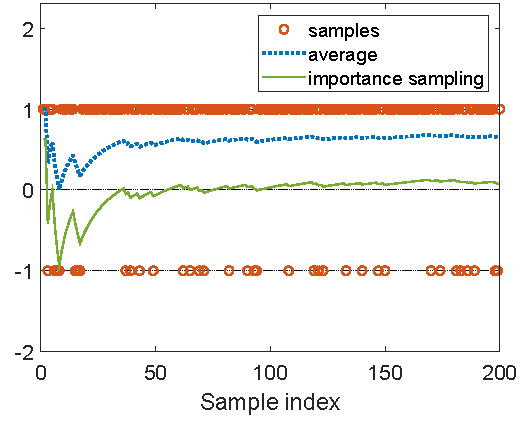
\includegraphics[width=255.2pt]{fig10_2}\par\smallskip
  \begin{minipage}{0.94\textwidth}\footnotesize
  \textbf{Figure 10.2.} An example for demonstrating the importance sampling technique. Here, X $\in$\{+1, $-$1\} and p0(X = +1) = p0(X = $-$1) = 0.5. The samples are generated according to p1 where p1(X = +1) = 0.8 and p1(X = $-$1) = 0.2. The average of the samples converges to EX$\sim$p1[X] = 0.6, but the weighted average calculated by the importance sampling technique in (10.10) converges to EX$\sim$p0[X] = 0.\par\smallskip
  \textcolor{rulegray}{\scriptsize Reproduced from S.~Zhao, \emph{Mathematical Foundations of Reinforcement Learning} (Springer, 2025).}
  \end{minipage}
\end{figure}


\subsubsection{The off-policy policy gradient theorem}

\bk{\S10.3.2, pp.~224--226; Theorem 10.1, p.~224; equation (10.11)}

Let $\beta$ be a behaviour policy and target
$J(\theta)=\sum_sd_\beta(s)v_\pi(s)=\E_{S\sim d_\beta}[v_\pi(S)]$.

\begin{theorem}[Off-policy policy gradient theorem, Theorem 10.1, p.~224]
For $\gamma\in(0,1)$,
\[
  \boxed{\;
  \nabla_\theta J(\theta)=\E_{S\sim\rho,\ A\sim\beta}
    \Bigl[\underbrace{\frac{\pi(A\mid S,\theta)}{\beta(A\mid S)}}_{\text{importance weight}}
      \nabla_\theta\ln\pi(A\mid S,\theta)\,q_\pi(S,A)\Bigr],\;}
\]
where $\rho(s)=\sum_{s'}d_\beta(s')\mathrm{Pr}_\pi(s\mid s')$ and
$\mathrm{Pr}_\pi(s\mid s')=[(I-\gamma P_\pi)^{-1}]_{s's}$.
\end{theorem}

Two differences from Theorem 9.1 \bkin{p.~224}: the importance weight, and
$A\sim\beta$ instead of $A\sim\pi$. That second change is the point --- we may now
use actions generated by $\beta$.

\subsubsection{The algorithm}

\bk{\S10.3.3, pp.~226--227; Algorithm 10.3, p.~226}

Baseline invariance survives the change (the same proof works), so subtract
$v_\pi(S)$ and replace the advantage by the TD error:
\[
  \theta_{t+1}=\theta_t+\alpha_\theta\frac{\pi(a_t\mid s_t,\theta_t)}{\beta(a_t\mid s_t)}
    \nabla_\theta\ln\pi(a_t\mid s_t,\theta_t)\,\delta_t(s_t,a_t).
\]

\begin{algobox}{Off-policy actor-critic via importance sampling (Algorithm 10.3, p.~226)}
\textbf{Initialise:} a behaviour policy $\beta(a\mid s)$; a target policy
$\pi(a\mid s,\theta_0)$; a value function $v(s,w_0)$; $\alpha_w,\alpha_\theta>0$.\\
At each time step $t$ of each episode:
\begin{itemize}\itemsep0pt
  \item Generate $a_t\sim\beta(\cdot\mid s_t)$, observe $r_{t+1},s_{t+1}$.
  \item \textbf{Advantage (TD error):}
        $\delta_t=r_{t+1}+\gamma v(s_{t+1},w_t)-v(s_t,w_t)$
  \item \textbf{Actor:}
        $\theta_{t+1}=\theta_t+\alpha_\theta\dfrac{\pi(a_t\mid s_t,\theta_t)}{\beta(a_t\mid s_t)}\,\delta_t\,\nabla_\theta\ln\pi(a_t\mid s_t,\theta_t)$
  \item \textbf{Critic:}
        $w_{t+1}=w_t+\alpha_w\dfrac{\pi(a_t\mid s_t,\theta_t)}{\beta(a_t\mid s_t)}\,\delta_t\,\nabla_w v(s_t,w_t)$
\end{itemize}
\end{algobox}

\begin{remark}
Algorithm 10.3 is Algorithm 10.2 with one extra factor in \emph{both} lines. Note
that the critic needs converting too, not just the actor: it is also estimating an
expectation under $\pi$ from data drawn under $\beta$
\bkin{\S10.3.3, p.~226}. Importance sampling is a general device and applies equally
to value-based methods \bkin{\S10.6 Q\&A, p.~236}.
\end{remark}

\subsection{Deterministic actor-critic (DPG)}

\bk{\S10.4, pp.~227--235; Theorem 10.2, p.~228; Algorithm 10.4, p.~234}

Every policy so far has been stochastic, because $\ln\pi$ requires
$\pi(a\mid s,\theta)>0$. Write a deterministic policy as
\[
  a=\mu(s,\theta),
\]
a \emph{mapping} $\Sspace\to\Aspace$ rather than a distribution
\bkin{\S10.4, p.~227}. Two reasons to care: it is \textbf{naturally off-policy}, and
it \textbf{handles continuous action spaces} --- where $\max_a$ and $\sum_a$ are not
available, so nothing from Chapters 7--8 applies.

\begin{theorem}[Deterministic policy gradient theorem, Theorem 10.2, p.~228; equation (10.14)]
\[
  \boxed{\;
  \nabla_\theta J(\theta)=\sum_{s\in\Sspace}\eta(s)\,\nabla_\theta\mu(s)\,
    \bigl(\nabla_a q_\mu(s,a)\bigr)\big|_{a=\mu(s)}
  =\E_{S\sim\eta}\Bigl[\nabla_\theta\mu(S)\bigl(\nabla_aq_\mu(S,a)\bigr)\big|_{a=\mu(S)}\Bigr].\;}
\]
\end{theorem}

\begin{intuition}[Read the chain rule]
$\nabla_aq_\mu$ says ``how much better would the value be if I nudged the action?''
and $\nabla_\theta\mu$ says ``how do I nudge the action by moving $\theta$?''.
Multiply them and you get how to move $\theta$ to raise the value. Nothing is
averaged over actions --- there is only one action per state.
\end{intuition}

\begin{remark}[Why it is off-policy, and a notation warning]
\bkin{\S10.4.1, p.~228}
The gradient contains \textbf{no action random variable $A$}. So estimating it
requires no action sampling, and any behaviour policy will do --- the deterministic
policy gradient method is off-policy by construction.

On notation: the book writes $\bigl(\nabla_aq_\mu(S,a)\bigr)|_{a=\mu(S)}$ rather
than $\nabla_aq_\mu(S,\mu(S))$ deliberately: the latter obscures which argument the
derivative is taken with respect to. A clearer compromise is
$\nabla_aq_\mu(S,a{=}\mu(S))$.
\end{remark}

\begin{algobox}{Deterministic actor-critic / DPG (Algorithm 10.4, p.~234)}
\textbf{Initialise:} a behaviour policy $\beta(a\mid s)$; a deterministic target
policy $\mu(s,\theta_0)$; a value function $q(s,a,w_0)$; $\alpha_w,\alpha_\theta>0$.\\
At each time step $t$ of each episode:
\begin{itemize}\itemsep0pt
  \item Generate $a_t\sim\beta$, observe $r_{t+1},s_{t+1}$.
  \item \textbf{TD error:}
        $\delta_t=r_{t+1}+\gamma q\bigl(s_{t+1},\mu(s_{t+1},\theta_t),w_t\bigr)-q(s_t,a_t,w_t)$
  \item \textbf{Actor:}
        $\theta_{t+1}=\theta_t+\alpha_\theta\nabla_\theta\mu(s_t,\theta_t)\bigl(\nabla_aq(s_t,a,w_t)\bigr)\big|_{a=\mu(s_t)}$
  \item \textbf{Critic:}
        $w_{t+1}=w_t+\alpha_w\,\delta_t\,\nabla_wq(s_t,a_t,w_t)$
\end{itemize}
\end{algobox}

\begin{warning}[Why no importance weight here?]
\bkin{\S10.4.2, p.~234} This is the subtlest point in the chapter. The critic is
off-policy, yet Algorithm 10.4 carries no importance weight, unlike Algorithm 10.3.
Why?

The critic's sample is $(s_t,a_t,r_{t+1},s_{t+1},\tilde a_{t+1})$ with
$\tilde a_{t+1}=\mu(s_{t+1})$. Two policies are involved: the one producing $a_t$
(that is $\beta$, the behaviour policy, since $a_t$ actually interacts with the
environment) and the one producing $\tilde a_{t+1}$ --- which is $\mu$, because $\mu$
is the policy the critic is evaluating. \textbf{But $\tilde a_{t+1}$ is never
executed}; it is only plugged into the TD target. So the target-policy action is
computed, not sampled, and there is no distribution mismatch to correct. Compare
Q-learning, off-policy for exactly the same structural reason: its $\max_a$ is
computed, not sampled \bkin{\S7.4.2, p.~142}.
\end{warning}

\begin{remark}[Practical choices, \bkin{\S10.4.2, p.~234}]
For $q(s,a,w)$, the original DPG paper used a linear function
$q(s,a,w)=\phi^{\!\top}(s,a)w$; modern practice uses neural networks, as in
\textbf{DDPG} (deep deterministic policy gradient). For $\beta$, any exploratory
policy works; a common choice is $\mu$ plus noise --- in which case $\mu$ is also the
behaviour policy and the implementation is effectively on-policy.
\end{remark}

\subsection{Chapter 10 summary}

\bk{\S10.5, pp.~235--236}

\begin{center}
\small
\begin{tabular}{@{}lp{0.58\textwidth}@{}}
\toprule
Algorithm & What it adds \\
\midrule
QAC (10.1) & Policy gradient with the $q$-estimate supplied by TD (Sarsa) instead of Monte Carlo. \\
A2C (10.2) & Subtracts the baseline $v_\pi(s)$, so the actor responds to the \emph{advantage}; the TD error estimates it with a single network. \\
Off-policy AC (10.3) & Importance weight $\pi/\beta$ in both actor and critic, so data from another policy can be used. \\
DPG (10.4) & Deterministic policy $a=\mu(s,\theta)$; naturally off-policy; handles continuous action spaces. Basis of DDPG. \\
\bottomrule
\end{tabular}
\end{center}

\begin{remark}[Where the subject goes from here]
\bkin{\S10.5, pp.~235--236} The book closes by pointing beyond itself: SAC, TRPO,
PPO and TD3 are advanced policy-gradient/actor-critic algorithms; multi-agent RL
extends the single-agent case; model-based RL fits a model from experience;
distributional RL replaces expected values with whole return distributions; and
there is a deep literature on the links between RL and control theory. Everything in
these ten chapters is the foundation those build on.
\end{remark}

\subsection{Chapter 10 self-check}

\begin{enumerate}
  \item In what precise sense is an actor-critic method both policy-based and
        value-based?
  \item Prove baseline invariance in three lines. Which property of probability
        distributions does the proof rest on?
  \item If the baseline does not change the gradient, why use one?
  \item Show that the TD error is an unbiased estimate of the advantage, and explain
        why this saves a network.
  \item Compute the importance weights in the coin example and verify that the
        weighted average converges to $0$ rather than $0.6$.
  \item Give an example where importance sampling fails, and state the condition that
        rules it out.
  \item Why does the deterministic policy gradient contain no action random variable,
        and why does that make it off-policy?
  \item Algorithm 10.3's critic carries an importance weight and Algorithm 10.4's does
        not, though both are off-policy. Explain the difference.
\end{enumerate}

\newpage

% ============================================================
\section*{Where everything fits}
\addcontentsline{toc}{section}{Where everything fits}
% ============================================================

A final map of the ten chapters. Read the table downward as a sequence of
assumptions being dropped.

\begin{center}
\small
\begin{tabular}{@{}llll@{}}
\toprule
Ch. & Contributes & Needs a model? & Representation \\
\midrule
1 & MDP: state, action, reward, return, policy & --- & --- \\
2 & State value $v_\pi$; the Bellman equation & yes (to solve it) & table \\
3 & Optimal values $v^*$; the BOE; contraction mapping & yes & table \\
4 & Value iteration, policy iteration, truncated PI & \textbf{yes} & table \\
5 & Monte Carlo: MC Basic, Exploring Starts, $\varepsilon$-greedy & no & table \\
6 & Robbins--Monro, Dvoretzky, SGD & --- & --- \\
7 & TD(0), Sarsa, $n$-step Sarsa, Q-learning & no & table \\
8 & Function approximation; TD-Linear; DQN & no & function (values) \\
9 & Policy gradient theorem; REINFORCE & no & function (policy) \\
10 & QAC, A2C, off-policy AC, DPG & no & function (both) \\
\bottomrule
\end{tabular}
\end{center}

\subsection*{The five ideas that recur everywhere}

\begin{enumerate}
  \item \textbf{Bootstrapping}, $G_t=R_{t+1}+\gamma G_{t+1}$ \bkin{\S1.6, p.~10}.
        It generates the Bellman equation (\S2.4), the TD target (\S7.1), the
        backward pass in MC Exploring Starts (\S5.3.3), and the advantage
        approximation in A2C (\S10.2.2).
  \item \textbf{Contraction}, $\norm{f(v_1)-f(v_2)}_\infty\le\gamma\norm{v_1-v_2}_\infty$
        \bkin{Theorem 3.2, p.~44}. It gives existence, uniqueness and an algorithm
        all at once, and the $\gamma$ reappears as the contraction constant in the
        convergence proofs of Chapter 7.
  \item \textbf{Generalised policy iteration}: alternate a value update and a policy
        update \bkin{\S4.4, p.~74}. Every algorithm in Chapters 4--10 has this shape;
        the actor and critic of Chapter 10 are its purest expression.
  \item \textbf{Stochastic approximation}: replace an unknown expectation by a
        sample, with step sizes satisfying $\sum a_k=\infty$, $\sum a_k^2<\infty$
        \bkin{Theorem 6.1, p.~106}. This is how every model-free algorithm is built.
  \item \textbf{Exploration}. It appears as a modelling choice ($\varepsilon$-greedy,
        \S5.4), as a hypothesis of convergence theorems ($\sum_t\alpha_t(s)=\infty$
        for every $s$, \S7.1.3), as a condition for the stationary distribution to
        exist (\S8.2.1), and as an automatic by-product of softmax policies
        (\S9.3). It is not an implementation detail; it is a structural requirement.
\end{enumerate}

\subsection*{A suggested study route}

\begin{enumerate}
  \item Watch the \vid{30-minute overview}{https://www.youtube.com/watch?v=ZHMWHr9811U}
        first, before reading anything.
  \item Read Chapters 1--3 carefully; they are short and everything else assumes them.
        Do the worked examples with pencil and paper.
  \item Chapter 4 is the pivot. If you understand that value iteration, policy
        iteration and truncated policy iteration are one algorithm with one dial,
        the rest of the book is a sequence of variations.
  \item Chapters 5 and 7 can be read as a pair: MC and TD are the two ways to
        estimate a value from data, and $n$-step Sarsa interpolates between them.
  \item Chapter 6 is machinery. Read \S6.1 and Theorem 6.1 properly; skim \S6.3 on
        first pass.
  \item Chapters 8--10 are modern RL. Read \S8.1 and \S9.1 slowly --- the conceptual
        shift from tables to functions is where most confusion arises.
  \item Run the code. The repository accompanying the textbook contains grid-world
        implementations in both MATLAB and Python; reproducing Figures 4.4, 7.2 and
        8.11 yourself is worth more than any amount of re-reading.
\end{enumerate}

\end{document}
